%%%%%%%%%%%%%%%%%%%%%%%%%%%%%%%%%%%%%%%%%
% SUTD Masters/Doctoral Thesis
% LaTeX Template
% Version 1.0 (29/08/16)
%
% Adapted to SUTD requirements by Martin Ochoa
%
% This template is based on a template downloaded from:
% http://www.LaTeXTemplates.com
%
% Version 2.x major modifications by:
% Vel (vel@latextemplates.com)
%
% which in turn was based on a template by:
% Steve Gunn (http://users.ecs.soton.ac.uk/srg/softwaretools/document/templates/)
% Sunil Patel (http://www.sunilpatel.co.uk/thesis-template/)
%
%
% Template license:
% CC BY-NC-SA 3.0 (http://creativecommons.org/licenses/by-nc-sa/3.0/)
%
%%%%%%%%%%%%%%%%%%%%%%%%%%%%%%%%%%%%%%%%%

%----------------------------------------------------------------------------------------
%	PACKAGES AND OTHER DOCUMENT CONFIGURATIONS

%----------------------------------------------------------------------------------------

\documentclass[
11pt, % The default document font size, options: 10pt, 11pt, 12pt
oneside, % Two side (alternating margins) for binding by default, uncomment to switch to one side
english, % ngerman for German
singlespacing, % Single line spacing, alternatives: onehalfspacing or doublespacing, singlespacing
%draft, % Uncomment to enable draft mode (no pictures, no links, overfull hboxes indicated)
%nolistspacing, % If the document is onehalfspacing or doublespacing, uncomment this to set spacing in lists to single
%liststotoc, % Uncomment to add the list of figures/tables/etc to the table of contents
%toctotoc, % Uncomment to add the main table of contents to the table of contents
%parskip, % Uncomment to add space between paragraphs
%nohyperref, % Uncomment to not load the hyperref package
headsepline, % Uncomment to get a line under the header
]{MastersDoctoralThesis} % The class file specifying the document structure

\usepackage[utf8]{inputenc} % Required for inputting international characters
\usepackage[T1]{fontenc} % Output font encoding for international characters

\usepackage{palatino} % Use the Palatino font by default

\usepackage[backend=bibtex,style=authoryear,natbib=true]{biblatex} % User the bibtex backend with the authoryear citation style (which resembles APA)

\addbibresource{example.bib} % The filename of the bibliography
\addbibresource{dgner.bib}
\addbibresource{depner.bib}
\addbibresource{dht.bib}
\addbibresource{incomp.bib}
\addbibresource{sql.bib}

\usepackage[autostyle=true]{csquotes} % Required to generate language-dependent quotes in the bibliography

\usepackage{color}

%----------------------------------------------------------------------------------------
%	MARGIN SETTINGS
%----------------------------------------------------------------------------------------

\geometry{
	paper=a4paper, % Change to letterpaper for US letter
	inner=2.54cm, % Inner margin
	outer=2.8cm, % Outer margin
	bindingoffset=1cm, % Binding offset
	top=2.5cm, % Top margin
	bottom=2.5cm, % Bottom margin
	%showframe,% show how the type block is set on the page
}

%----------------------------------------------------------------------------------------
%	THESIS INFORMATION
%----------------------------------------------------------------------------------------

\thesistitle{Leveraging Dependency Trees for Structured Prediction} % Your thesis title, this is used in the title and abstract, print it elsewhere with \ttitle
%Exploiting the Potential of Dependency Structures
\supervisor{Prof. Wei \textsc{Lu}} % Your supervisor's name, this is used in the title page, print it elsewhere with \supname
\examiner{} % Your examiner's name, this is not currently used anywhere in the template, print it elsewhere with \examname
\degree{Doctor of Philosophy} % Your degree name, this is used in the title page and abstract, print it elsewhere with \degreename
\author{Zhanming \textsc{Jie}} % Your name, this is used in the title page and abstract, print it elsewhere with \authorname
\addresses{} % Your address, this is not currently used anywhere in the template, print it elsewhere with \addressname
\university	{SUTD}
\keywords{} % Keywords for your thesis, this is not currently used anywhere in the template, print it elsewhere with \keywordnames
\pillar{Information Systems Technology and Design} % Pillar

\hypersetup{pdftitle=\ttitle} % Set the PDF's title to your title
\hypersetup{pdfauthor=\authorname} % Set the PDF's author to your name
\hypersetup{pdfkeywords=\keywordnames} % Set the PDF's keywords to your keywords

\usepackage{amsmath}
\usepackage{multirow}
\usepackage{adjustbox}

\usepackage{graphicx}  %Required
\usepackage{amsfonts}
\usepackage{subcaption}

\renewcommand{\vec}[1]{\mathbf{#1}} %make vector symbol bold
\DeclareMathOperator*{\argmin}{arg\,min}
\DeclareMathOperator*{\argmax}{arg\,max}
%\DeclareMathOperator*{\len}{len}
\usepackage{footnote}
\usepackage{epstopdf}
\usepackage{algorithm} %algorithm package
\usepackage{algpseudocode} %algorithm
\usepackage{stmaryrd}
\usepackage{booktabs,arydshln}
\usepackage{mathtools}

\usepackage{color}
\usepackage{tikz}
\usepackage{pgf}
\usepackage{pgfplots}
\usepackage{tikz-qtree}
\usetikzlibrary{arrows,decorations.pathmorphing,backgrounds,positioning,fit,petri,shapes.misc, arrows.meta,shapes.geometric,decorations.markings,calc,shadows.blur,decorations.pathreplacing,quotes,matrix,shapes.symbols}
\tikzset{->-/.style={decoration={
			markings,
			mark=at position 0.5 with {\arrow{>}}},postaction={decorate}}}
\tikzset{->--/.style={decoration={
			markings,
			mark=at position 0.4 with {\arrow{>}}},postaction={decorate}}}

\definecolor{fontgray}{RGB}{44, 62, 80}
\definecolor{myred}{RGB}{235, 47, 6} %rgb()
\definecolor{summertime}{RGB}{245, 205, 121}
\definecolor{darkgrass}{RGB}{0, 148, 50}
\definecolor{myblue}{RGB}{0, 168, 255}
\definecolor{mygray}{RGB}{158, 158, 158}
\definecolor{puffin}{RGB}{250, 152, 58}
\definecolor{lowpurple}{RGB}{210, 180, 222}
\definecolor{lowblue}{RGB}{102,178,255}
\definecolor{lowred}{RGB}{245, 183, 177}
\definecolor{darkblue}{rgb}{0, 0, 0.5}

\definecolor{grass}{RGB}{0, 148, 50}
\definecolor{mypurple}{RGB}{108, 92, 231}

\def\pnode [#1]#2{
	% node for the potential function
	\node[regular polygon,regular polygon sides=4, minimum size=1pt,fill=gray,#1, inner sep = 1.2pt] (#2) {};
} 
\tikzset{middlefactor/.style={decoration={
			markings,
			mark= at position #1 with {\pnode[]{}} 
		},postaction={decorate}},
	middlefactor/.default=0.5
}

\renewcommand{\cite}{\parencite}
\newtheorem{theorem}{Theorem}%[section]
\newtheorem{lemma}[theorem]{Lemma}
\newtheorem{proposition}[theorem]{Proposition}
\newtheorem{corollary}[theorem]{Corollary}

\newenvironment{proof}[1][Proof]{\begin{trivlist}
		\item[\hskip \labelsep {\bfseries #1}]}{\end{trivlist}}
\newenvironment{definition}[1][Definition]{\begin{trivlist}
		\item[\hskip \labelsep {\bfseries #1}]}{\end{trivlist}}
\newenvironment{assumption}[1][Assumption]{\begin{trivlist}
		\item[\hskip \labelsep {\bfseries #1}]}{\end{trivlist}}
\newenvironment{example}[1][Example]{\begin{trivlist}
		\item[\hskip \labelsep {\bfseries #1}]}{\end{trivlist}}
\newenvironment{remark}[1][Remark]{\begin{trivlist}
		\item[\hskip \labelsep {\bfseries #1}]}{\end{trivlist}}

\newcommand{\qed}{\nobreak \ifvmode \relax \else
	\ifdim\lastskip<1.5em \hskip-\lastskip
	\hskip1.5em plus0em minus0.5em \fi \nobreak
	\vrule height0.65em width0.5em depth0.25em\fi}

\makeatletter
\def\adl@drawiv#1#2#3{%
	\hskip.5\tabcolsep
	\xleaders#3{#2.5\@tempdimb #1{1}#2.5\@tempdimb}%
	#2\z@ plus1fil minus1fil\relax
	\hskip.5\tabcolsep}
\newcommand{\cdashlinelr}[1]{%
	\noalign{\vskip\aboverulesep
		\global\let\@dashdrawstore\adl@draw
		\global\let\adl@draw\adl@drawiv}
	\cdashline{#1}
	\noalign{\global\let\adl@draw\@dashdrawstore
		\vskip\belowrulesep}}
\def\blfootnote{\xdef\@thefnmark{}\@footnotetext}
\makeatother

\begin{document}

\frontmatter % Use roman page numbering style (i, ii, iii, iv...) for the pre-content pages

\pagestyle{plain} % Default to the plain heading style until the thesis style is called for the body content

%----------------------------------------------------------------------------------------
%	TITLE PAGE
%----------------------------------------------------------------------------------------

\begin{titlepage}
\begin{center}

\begin{figure}
\centering

\includegraphics[width=0.5\textwidth]{Figures/SUTD}
\end{figure}

 \hfill\break\\[2.3cm]

{\huge \bfseries \ttitle}\\[2cm] % Thesis title


Submitted by\\[1cm]
\authorname % Author name - remove the \href bracket to remove the link

\vspace{4em}

Thesis Advisor\\[1cm]
\supname % Supervisor name - remove the \href bracket to remove the link

\vspace{4em}

\pillarname\\[1.5cm] % Research group name and department name

\large{A thesis submitted to the Singapore University of Technology and Design in fulfillment of the requirement for the degree of \degreename}\\[1cm] % University requirement text


{\large \the\year}\\[4cm] % Date
%\includegraphics{Logo} % University/department logo - uncomment to place it

\vfill
\end{center}
\end{titlepage}

%----------------------------------------------------------------------------------------
%	DECLARATION PAGE
%----------------------------------------------------------------------------------------

\begin{tec}
\addchaptertocentry{\tecname}
\begin{tabular}{ll}
	TEC Chair: & Prof. Ngai-Man Cheung \\
	Main Advisor: & Prof. Wei Lu \\
%	Co-advisor(s): & Prof. XXXX (if any) \\
	Internal TEC member 1: & Prof. Shaowei Lin \\
	Internal TEC member 2: & Prof. Dario Poletti \\
	External TEC member 1: & Prof. Jing Jiang (Singapore Management University) \\
%	External TEC member 2: & Prof. XXXX (optional) \\
\end{tabular}
\end{tec}
\vfill\eject

%----------------------------------------------------------------------------------------
%	DECLARATION PAGE
%----------------------------------------------------------------------------------------

%\begin{declaration}
%\addchaptertocentry{\authorshipname}
%
%% \noindent I, \authorname, declare that this thesis titled, \enquote{\ttitle} and the work presented in it are my own. I confirm that:
%%
%% \begin{itemize}
%% \item This work was done wholly or mainly while in candidature for a research degree at this University.
%% \item Where any part of this thesis has previously been submitted for a degree or any other qualification at this University or any other institution, this has been clearly stated.
%% \item Where I have consulted the published work of others, this is always clearly attributed.
%% \item Where I have quoted from the work of others, the source is always given. With the exception of such quotations, this thesis is entirely my own work.
%% \item I have acknowledged all main sources of help.
%% \item Where the thesis is based on work done by myself jointly with others, I have made clear exactly what was done by others and what I have contributed myself.\\
%% \end{itemize}
%
%I hereby confirm the following:
%\begin{itemize}
%\item I hereby confirm that the thesis work is original and has not been submitted to any other University or Institution for higher degree purposes.
%\item I hereby grant SUTD the permission to reproduce and distribute publicly paper and electronic copies of this thesis document in whole or in part in any medium now known or hereafter created in accordance with Policy on Intellectual Property, clause 4.2.2.
%\item I have fulfilled all requirements as prescribed by the University and provided 1 copy of my thesis in PDF.
%\item I have attached all publications and award list related to the thesis (e.g. journal, conference report and patent).
%\item The thesis does / does not (delete accordingly) contain patentable or confidential information.
%\item I certify that the thesis has been checked for plagiarism via turnitin/ithenticate. The score is 100\%.
%\end{itemize}
%
%\noindent Name and signature:\\
%\rule[0.5em]{25em}{0.5pt} % This prints a line for the signature
%
%\noindent Date:\\
%\rule[0.5em]{25em}{0.5pt} % This prints a line to write the date
%\end{declaration}

%\vfill
\cleardoublepage

%----------------------------------------------------------------------------------------
%	QUOTATION PAGE
%----------------------------------------------------------------------------------------

% Uncomment for quotation page
 \vspace*{0.2\textheight}

 \noindent\enquote{\itshape When you embrace stress, you can transform fear into courage, isolation into connection, and suffering into meaning.}\bigbreak

 \hfill Kelly McGonigal

%----------------------------------------------------------------------------------------
%	ABSTRACT PAGE
%----------------------------------------------------------------------------------------

\begin{abstract}
\addchaptertocentry{\abstractname} % Add the abstract to the table of contents



Syntactic dependency structures leverage shallow semantic information, which could be helpful for downstream tasks in natural language processing (NLP). 
In this thesis, we present some of our recent works on improving named entity recognition (NER) and semantic parsing by making use of the rich structured information in the dependency trees. 
We statistically show the strong correlation between the dependency trees and named entities. 
Specifically, named entities often form subtrees under the dependency tree structures, and the dependency relations (e.g. \textit{nsubj}) are strong indicators for the existence of entities. 
Motivated by the above observations, we proposed the dependency-guided structured models based on the conditional random fields (CRF) to capture the underlying correlations for the NER task. 
Our large-scale experiments on four languages demonstrate the effectiveness of the proposed model, especially for the Catalan and Spanish languages. 
Further analysis reveals that the improvements mainly result from the dependency relations and long-distance interactions provided by dependency trees.

Our following research work attacks a more challenging and semantic-level task, semantic parsing without the given dependency trees. 
The semantic parsing task is to map the natural language sentences into (tree-structured) logical forms. 
We introduce a dependency-based hybrid tree representation to capture the interactions between the semantic units and the natural language words.
However, as the dependency trees are not observed, we regard the dependency trees as the latent structures in our proposed latent-variable model. 
Our dynamic-programming inference procedure is similar to the Eisner's algorithm for dependency parsing. 
The proposed model achieves state-of-the-art performance on 7 out of 8 languages, especially for some datasets with flexible word order. 

%The core of these proposed models are based on structured prediction. 
%Different structured prediction models 

{\paragraph{Keyword:} Dependency Trees, Structured Prediction, Named Entity Recognition, Semantic Parsing, Dynamic Programming
}

%The Thesis Abstract is written here (and usually kept to just this page). The page is kept centered vertically so can expand into the blank space above the title too\ldots

\end{abstract}

%----------------------------------------------------------------------------------------
%	Publications
%----------------------------------------------------------------------------------------

\begin{publications}
\addchaptertocentry{\publicationsname} % Add the abstract to the table of contents

\begin{itemize}
	\item \textbf{Zhanming Jie} and Wei Lu. 2019. Dependency-Guided LSTM-CRF for Named Entity Recognition. In \textit{Proceedings of EMNLP.}
	\item \textbf{Zhanming Jie}, Pengjun Xie, Wei Lu, Ruixue Ding and Linlin Li. 2019. Better Modeling of Incomplete Annotations for Named Entity Recognition. In \textit{Proceedings of NAACL.}
	\item \textbf{Zhanming Jie} and Wei Lu. 2018. Dependency-based Hybrid Tree for Semantic Parsing. In \textit{Proceedings of EMNLP.}
	\item Chu Guo, \textbf{Zhanming Jie}, Wei Lu and Dario Poletti. 2018. Matrix Product Operators for Sequence to Sequence Learning. In \textit{Physical Review E.}
	\item \textbf{Zhanming Jie}, Aldrian Obaja Muis, and Wei Lu. 2017. Efficient Dependency-Guided Named Entity Recognition. In \textit{Proceedings of the AAAI.}
	\item \textbf{Zhanming Jie}, Ming Cheung, and James She. A Cloud-Assisted Framework for Bag-of-Features Tagging in Social Networks. 2015. In \textit{IEEE Fourth Symposium on Network Cloud Computing and Applications.}
	\item Alvin Junus, Ming Cheung, James She, and \textbf{Zhanming Jie}. 2015. Community-Aware Prediction of Virality Timing Using Big Data of Social Cascades. In \textit{Proceedings of IEEE BigDataService.}
	\item Ming Cheung, James She, and \textbf{Zhanming Jie}. 2015. Connection Discovery Using Big Data of User-Shared Images in Social Media. In \textit{IEEE Transactions on Multimedia.}
	\item \textbf{Zhanming Jie} and Wei Lu. 2014. Multilingual Semantic Parsing: Parsing Multiple Languages into Semantic Representations. In \textit{Proceedings of COLING.}
\end{itemize}

\end{publications}

%----------------------------------------------------------------------------------------
%	ACKNOWLEDGEMENTS
%----------------------------------------------------------------------------------------

\begin{acknowledgements}
\addchaptertocentry{\acknowledgementname} % Add the acknowledgements to the table of contents

First and foremost, I'm very grateful to have Prof. Wei Lu as my PhD advisor. 
Without a doubt, I have a lot of for him.
What I have learned from him during these years will benefit me for the rest of my life.  
He is the person who is sincerely serious about research, which really impresses me.
I first met Prof. Wei Lu in 2014 when I did my internship with him and I knew nothing about NLP. 
%He worked day and night and often went home at around 3 am. 
He is extremely efficient and focused during working. 
He taught me what correct attitude is to research, how to do good research in terms of reading, writing, my presentation skill, and more importantly, how to think independently as a researcher. 
All of the things that he endowed me and I have learned from him can not be simply stated in a few sentences. 
But I really appreciate that I can spend these four years with him. 


I would like to thank my mother and brother for their support during my PhD study. 
They do not give me pressure and support most of the decisions I made, though my mom is sometimes a bit immature and she is the ``funniest'' one in the family.
When I get into trouble like mental problems, I often seek help from my brother.  
Talking to him makes me feel better and he is the one usually talks a lot though what he said is not really helpful. 
I really enjoy the happiness and joy in this family.

Throughout my PhD study, there are a lot of friends who have provided their help to me. 
Aldrian, who was previously a research assistant in our group, gave me tremendous guidance in my first year. 
He is a really smart and also very friendly teacher to me. 
Raymond and Li Hao had a lot of research discussions with me during my PhD study. 
Besides research, we chat with each other on our PhD life. 
I really appreciate the conversations with them as it sometimes helps me get away from the pressure of ``tough'' research.
Gary and I joined the PhD program together back to Jan 2016. 
Yuqi and Gary are my best friends since I join SUTD. 
We took classes together, played together and talk about everything. 
I really appreciate the time that we spent in our PhD study and wish them a promising fortune in the future. 
Of course, there are so many friends and team members that I haven't mentioned but I'm really grateful for their appearance in my life. 
PhD life sometimes is tough. 
Because of them, it makes my life more fun and more wonderful. 

After finishing the defense, I really appreciate Prof. Jiang Jing for her comments on this thesis. 
I have a lot respect to her in the field of natural language processing. 
She read through the thesis and wrote many useful comments especially some of them are really inspiring for my future research direction. 
I would also love to work with Prof. Jiang Jing in the future. 

Last but certainly not least, I would like to thank the one inside my heart (\textit{i.e.}, myself) for insisting on the PhD study. 
Four years ago, you had already gone through 1-year PhD life and I know that was a really tough and stressed time for you.
Thus, you quit that PhD and Prof. Wei Lu gave you a second chance to demonstrate yourself. 
But I know you were still very stressed and somehow you might have lost your faith in doing the PhD. 
You were even thinking that you do not have any talents in doing research. 
Though you published some papers, you also failed so many research topics. 
After several failures, you doubted yourself, questioned yourself and denied yourself that you can do a good job. 
Later on, you realized that it is not about just research and publishing papers. 
You realized that you love doing research, especially good research.
No matter if you can publish in the top conference or not, you still love doing research. 
As your advisor requires, I hope  you are already an independent researcher now. 
I hope you can keep doing great research in the future and do not forget your original motivation for doing a PhD.








\end{acknowledgements}

%----------------------------------------------------------------------------------------
%	LIST OF CONTENTS/FIGURES/TABLES PAGES
%----------------------------------------------------------------------------------------

\tableofcontents % Prints the main table of contents

\listoffigures % Prints the list of figures

\listoftables % Prints the list of tables

%----------------------------------------------------------------------------------------
%	ABBREVIATIONS
%----------------------------------------------------------------------------------------

% Uncomment for abbreviations page
 \begin{abbreviations}{ll} % Include a list of abbreviations (a table of two columns)

	 \textbf{NLP} & \textbf{N}atural  \textbf{L}anguage \textbf{P}rocessing\\
 \textbf{NER} & \textbf{N}amed \textbf{E}entity \textbf{R}ecognition\\
  \textbf{HMM} & \textbf{H}idden \textbf{M}arkov \textbf{M}odel\\
    \textbf{MEMM} & \textbf{M}aximum \textbf{E}ntropy \textbf{M}arkov \textbf{M}odel\\
 \textbf{CRF} & \textbf{C}onditional \textbf{R}andom \textbf{F}ield\\
 \textbf{LSTM} & \textbf{L}ong \textbf{S}ort-\textbf{T}erm \textbf{M}emory\\
\textbf{DGM} & \textbf{D}ependency-\textbf{G}uided \textbf{M}odel\\
\textbf{SQL} & \textbf{S}tructured \textbf{Q}uery \textbf{L}anguage\\
\textbf{AMR} & \textbf{A}bstract \textbf{M}eaning \textbf{R}epresentation\\
\textbf{DGLSTM} & \textbf{D}ependency \textbf{G}uided LSTM\\
\textbf{NL} & \textbf{N}atural \textbf{L}anguage \\
\textbf{MR} & \textbf{M}eaning \textbf{R}epresentation \\
\textbf{MST} & \textbf{M}aximum \textbf{S}panning \textbf{T}ree \\
\textbf{GCN} & \textbf{G}raph \textbf{C}onvolutional \textbf{N}etwork \\



 \end{abbreviations}

%----------------------------------------------------------------------------------------
%	PHYSICAL CONSTANTS/OTHER DEFINITIONS
%----------------------------------------------------------------------------------------

% Uncomment for physical constants etc
% \begin{constants}{lr@{${}={}$}l} % The list of physical constants is a three column table
%
% % The \SI{}{} command is provided by the siunitx package, see its documentation for instructions on how to use it
%
% 	Speed of Light & $c_{0}$ & \SI{2.99792458e8}{\meter\per\second} (exact)\\
% %Constant Name & $Symbol$ & $Constant Value$ with units\\
%
% \end{constants}

%----------------------------------------------------------------------------------------
%	SYMBOLS
%----------------------------------------------------------------------------------------

% Uncomment for symbols
% \begin{symbols}{lll} % Include a list of Symbols (a three column table)
%
% $a$ & distance & \si{\meter} \\
% $P$ & power & \si{\watt} (\si{\joule\per\second}) \\
% %Symbol & Name & Unit \\
%
% \addlinespace % Gap to separate the Roman symbols from the Greek
%
% $\omega$ & angular frequency & \si{\radian} \\
%
% \end{symbols}

%----------------------------------------------------------------------------------------
%	DEDICATION
%----------------------------------------------------------------------------------------

\dedicatory{To my mom and brother, for their endless support.}

%----------------------------------------------------------------------------------------
%	THESIS CONTENT - CHAPTERS
%----------------------------------------------------------------------------------------

\mainmatter % Begin numeric (1,2,3...) page numbering

\pagestyle{thesis} % Return the page headers back to the "thesis" style

% Include the chapters of the thesis as separate files from the Chapters folder
% Uncomment the lines as you write the chapters

% Chapter 1

\chapter{Introduction} % Main chapter title

\label{Chapter1} % For referencing the chapter elsewhere, use \ref{Chapter1} 

%----------------------------------------------------------------------------------------

% Define some commands to keep the formatting separated from the content 
\newcommand{\keyword}[1]{\textbf{#1}}
\newcommand{\tabhead}[1]{\textbf{#1}}
\newcommand{\code}[1]{\texttt{#1}}
\newcommand{\file}[1]{\texttt{\bfseries#1}}
\newcommand{\option}[1]{\texttt{\itshape#1}}

%----------------------------------------------------------------------------------------

\section{Dependency Trees}
Dependency trees describe the bilexical relations between pairs of words in a sentence. 
Such relations are drawn from a fixed inventory of grammatical relations~\parencite{jurafsky2000speech}.
For example, Figure \ref{fig:example} shows an example sentence (taken from OntoNotes 5.0~\cite{weischedel2013ontonotes}) with dependency annotations to describe the bilexical relationship between pairs of words. 
\begin{figure}[h!]
	\centering
	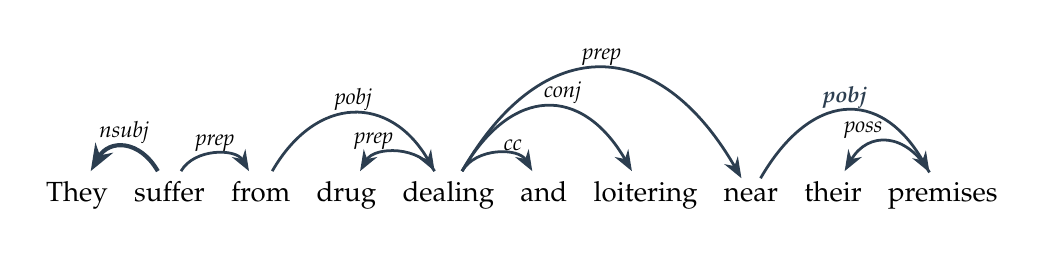
\begin{tikzpicture}[node distance=1.0mm and 1.0mm, >=Stealth, 
	wordnode/.style={draw=none, minimum height=5mm, inner sep=0pt},
	chainLine/.style={line width=1pt,-, color=fontgray},
	entbox/.style={draw=black, rounded corners, fill=red!20, dashed}
	]
	\matrix (sent1) [matrix of nodes, nodes in empty cells, execute at empty cell=\node{\strut};]
	{
		They & [1mm]suffer &[1mm]from & [1mm]drug   &  [1mm]  dealing & [1mm]and& [1mm]loitering& [1mm]near & [1mm]their & [1mm]premises\\
	};
	
	\draw [chainLine, ->, color=fontgray, line width=1.5pt] (sent1-1-2) to [out=120,in=60, looseness=1.4] node[above, yshift=-1mm, color=black]{\footnotesize\it nsubj} (sent1-1-1);
	\draw [chainLine, ->] (sent1-1-2) to [out=60,in=120, looseness=1] node[above, yshift=-1mm, color=black]{\footnotesize\it prep} (sent1-1-3);
	\draw [chainLine, ->] (sent1-1-5) to [out=120,in=60, looseness=1] node[above, yshift=-1mm, xshift=-3mm, color=black]{\footnotesize\it prep} (sent1-1-4);
	\draw [chainLine, ->] (sent1-1-3) to [out=60,in=120, looseness=1.4] node[above, yshift=-1mm, color=black]{\footnotesize\it pobj} (sent1-1-5);
	\draw [chainLine, ->] (sent1-1-5) to [out=60,in=120, looseness=1] node[above, yshift=-1mm, color=black, xshift=2mm]{\footnotesize\it cc} (sent1-1-6);
	\draw [chainLine, ->] (sent1-1-5) to [out=60,in=120, looseness=1.5] node[above, yshift=-1mm, color=black, xshift=2mm]{\footnotesize\it conj} (sent1-1-7);
	\draw [chainLine, ->] (sent1-1-5) to [out=60,in=120, looseness=1.5] node[above, yshift=-1mm, color=black]{\footnotesize\it prep} (sent1-1-8);
	\draw [chainLine, ->, color=fontgray, line width=1pt] (sent1-1-10) to [out=120,in=60, looseness=1.4] node[above, yshift=-1mm, color=black, xshift=-3mm]{\footnotesize\it poss} (sent1-1-9);
	\draw [chainLine, ->, line width=1pt] (sent1-1-8) to [out=60,in=120, looseness=1.5] node[above, yshift=-1mm]{\footnotesize\textit{\textbf{pobj}} } (sent1-1-10);		
	\end{tikzpicture} 
	\caption{Example sentences annotated with dependency structures.}
	\label{fig:example}
\end{figure}

The word ``\textit{They}'' is the subject of the verb ``\textit{suffer}'', and ``\textit{from}'' is the preposition of this verb. 
Overall, we can see that each word has exactly one parent as in the dependency trees except for the root (i.e., ``\textit{suffer}'' in this case).
On the other hand, this tree is \textbf{\textit{projective}} in the sense that there is no crossing edge in the dependency trees. 
According to \citet{jurafsky2000speech}, an arc from a head to a dependent is said to be projective if there is a path from the head to every word that lies between the head and the dependent in the sentence. 
A dependency tree is then said to be projective if all the arcs that make it up are projective. 
Most of the dependency trees in English are projective while non-projective dependencies are also allowed, particularly for some languages with flexible word orders, such as Czech.

As different languages have different forms of dependencies as well as different types of dependency relations, \textit{Universal Dependencies}\footnote{https://universaldependencies.org/}~\cite{nivre2016universal} are proposed to consistently unify the grammar across different languages.
%As of today, there are 157 treebanks for 90 languages. 
The speedy progress of universal dependencies allows us to work on the downstream tasks by making use of such dependency trees. 


%----------------------------------------------------------------------------------------

\section{Motivation}



%%% rough motivation
Motivated by the fact that the dependency trees convey semantic-level information, we focus on the structured prediction tasks of named entity recognition~\cite{tjong2003introduction} and semantic parsing which requires a semantic-level understanding of natural languages. 
Specifically, we study the underlying connections between the dependency trees and the output structures (\textit{e.g.}, named entity sequences and structured meaning representation) based on our observation from existing datasets. 
We raise several research questions in this thesis for us to exploit the connections for the downstream tasks. 


\subsection{Dependency-Guided Named Entity Recognition}
Though the dependencies describe the bilexical relations between pairs of words, we should be aware that some words that form a named entity should be treated as a \textit{complete} unit in the dependency trees. 
For example, the \textsc{gpe} entity ``\textit{Hong Kong}'' is a complete unit and it should form a subtree in the following example. 
The same applies to the \textsc{event} entity ``\textit{seminar on the actual practice of tax reform}''. 

\begin{figure}[h!]
	\centering
	%	\includegraphics[width=2.8in]{imgs/example.pdf}
	\adjustbox{max width=1.0\linewidth}{
		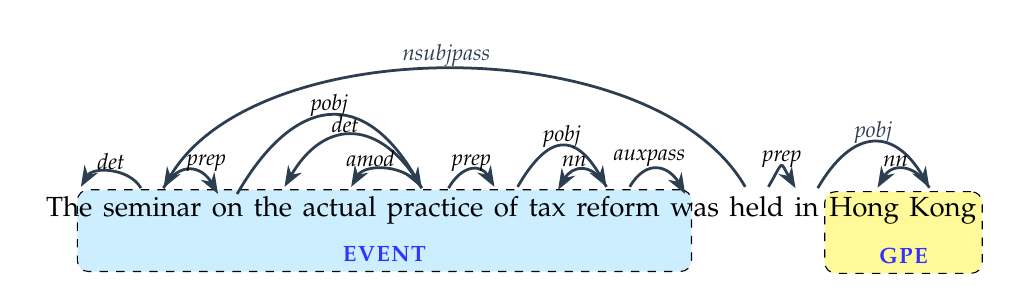
\begin{tikzpicture}[node distance=1.0mm and 1.0mm, >=Stealth, 
		wordnode/.style={draw=none, minimum height=5mm, inner sep=0pt},
		chainLine/.style={line width=1pt,-, color=fontgray},
		entbox/.style={draw=black, rounded corners, fill=red!20, dashed}
		]
	
		
		
		\matrix (sent2) [matrix of nodes, nodes in empty cells, execute at empty cell=\node{\strut};]
		{
			The &[-1mm] seminar &[-1mm] on &[-1mm] the & [-1mm]actual   &    [-1mm]practice &[-1mm] of & [-1mm]tax& [-1mm]reform & [-1mm]was & [-1mm]held & [-1mm]in &[-1mm] Hong &[-1mm] Kong\\
			%		 \textbf{\textsc{date}}   &   &   & \textsc{o}     & \textsc{o}   & \textsc{o}  & \textsc{o}& \textsc{event} &  \\
		};
		
		\draw [chainLine, ->] (sent2-1-2) to [out=120,in=60, looseness=1] node[above, yshift=-1mm, xshift=0mm,  color=black]{\footnotesize\it det} (sent2-1-1);
		\draw [chainLine, <-] (sent2-1-3) to [out=120,in=60, looseness=1.5] node[above, yshift=-1.5mm,  color=black, xshift=2mm]{\footnotesize\it prep} (sent2-1-2);
		\draw [chainLine, ->] (sent2-1-6) to [out=120,in=60, looseness=1.5] node[above, yshift=-1mm, xshift=-1mm,  color=black]{\footnotesize\it det} (sent2-1-4);
		\draw [chainLine, ->] (sent2-1-6) to [out=120,in=60, looseness=1] node[above, yshift=-1mm, xshift=-2mm,  color=black]{\footnotesize\it amod} (sent2-1-5);
		\draw [chainLine, ->] (sent2-1-3) to [out=60,in=120, looseness=1.6] node[above, yshift=-1.5mm,  color=black]{\footnotesize\it pobj} (sent2-1-6);
		\draw [chainLine, ->] (sent2-1-6) to [out=60,in=120, looseness=1.5] node[above, yshift=-1.5mm,  color=black]{\footnotesize\it prep} (sent2-1-7);
		\draw [chainLine,<-, line width=1pt] (sent2-1-8) to [out=60,in=120, looseness=1.5] node[above, yshift=-1mm, color=black,xshift=-1mm]{\footnotesize\it nn} (sent2-1-9);
		\draw [chainLine, ->] (sent2-1-7) to [out=60,in=120, looseness=1.8] node[above, yshift=-1.5mm,  color=black]{\footnotesize\it pobj} (sent2-1-9);
		
		\draw [chainLine,->, line width=1pt] (sent2-1-9) to [out=60,in=120, looseness=1.5] node[above, yshift=-1mm, color=black,xshift=-1mm]{\footnotesize\it auxpass} (sent2-1-10);
		\draw [chainLine, ->] (sent2-1-11) to [out=60,in=120, looseness=3.0] node[above, yshift=-1.5mm,  color=black]{\footnotesize\it prep} (sent2-1-12);
		
		\draw [chainLine, ->, color=fontgray, line width=1pt] (sent2-1-12) to [out=60,in=120, looseness=1.6] node[above, yshift=-1.5mm,  color=fontgray]{\footnotesize\it pobj} (sent2-1-14);
		\draw [chainLine, <-] (sent2-1-13) to [out=60,in=120, looseness=1.4] node[above, yshift=-1mm,  color=black, xshift=-1mm]{\footnotesize\it nn} (sent2-1-14);
		
		\draw [chainLine, <-, color=fontgray, line width=1pt] (sent2-1-2) to [out=60,in=120, looseness=0.8] node[above, yshift=-1mm,  color=fontgray, xshift=-1mm]{\footnotesize\it nsubjpass} (sent2-1-11);
		
		
		\begin{pgfonlayer}{background}
		\node [entbox, below=of sent2-1-5, xshift=5.7mm, yshift=5.8mm, text height=8mm, minimum width=78mm, fill=myblue!20] (e2)  [] {\color{blue!80}\textbf{\textsc{event}}};
		\node [entbox, below=of sent2-1-13, xshift=5mm, yshift=6.5mm, text height=8mm, minimum width=20mm, fill=yellow!40] (e2)  [] {\color{blue!80}\textbf{\textsc{gpe}}};
		\end{pgfonlayer}
		\end{tikzpicture} 
	}
	%	\vspace*{-7.5mm}
	\caption{Example sentences annotated with named entities and dependencies in the OntoNotes 5.0 dataset.}
	%	\vspace*{-6mm}
	\label{fig:examples}
\end{figure}

By observing the named entity datasets with dependency annotations, we found that most of the entities often form dependency subtrees in a sentence~\cite{jie2017efficient}. 
On the other hand, certain entities have strong correlations with the dependency relations~\cite{jie2019dependency}. 
For example, in the OntoNotes dataset~\cite{weischedel2013ontonotes}, 61\% of \textsc{norp} (i.e., Nationalities or religious or political groups) entities attach to the dependency relations \textit{amod} (i.e., adjectival modifier). 

The major research challenge is how we can make use of these two types of relationships to improve our named entity recognition systems. 
We ask the following three research questions: 
\begin{itemize}
	\item \textit{We know entities form subtrees in the dependencies. Can we impose certain constraints in the NER models to filter out some candidates that cannot form subtrees?}
	\item \textit{Besides, how to incorporate the complete structured information provided by the dependency trees for NER?}
	\item \textit{What if we do not have the complete annotations for NER? How does the dependency help in such a scenario?}
\end{itemize}

We aim to design efficient models to solve these two research questions and capture the complete structured information in our model architecture~\cite{jie2017efficient,jie2019dependency}. 
The third question is an actual incomplete annotation scenario~\cite{jie2019better} and the relationship between the dependency and named entities may take a role in such a scenario. 

\subsection{Dependencies in Semantic Parsing}
Semantic parsing is a fundamental task within the field of natural language processing (NLP).
Semantic parsing aims to transform the natural language sentences into machine-interpretable meaning representations automatically. 
On the other hand, the previous work~\cite{reddy2016transforming} shows that dependency trees leverage shallow semantic information. 

\begin{figure}[h!]
	\centering
	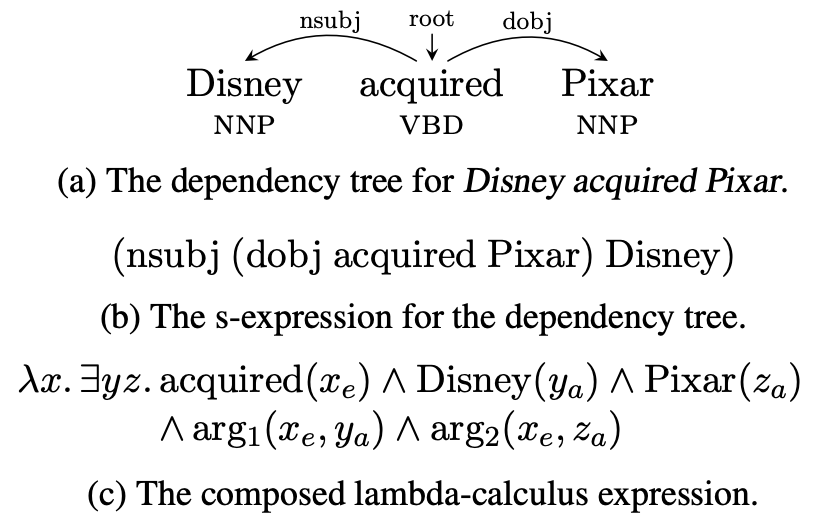
\includegraphics[width=4in]{Figures/dep2lambda.png}
	\caption{Example of transforming dependency into logical forms (taken from \citet{reddy2016transforming}).}
	\label{fig:transformexample}
\end{figure}

The underlying observation is helpful for extracting semantic meaning representation from the dependency trees. 
\citet{reddy2016transforming,reddy2017universal} proposed a supervised learning approach to transform the universal dependencies into lambda-calculus expression. 
Similarly, \citet{wang2015transition} proposed a transition-based algorithm to convert the dependency trees into abstract meaning representations (AMR).
Universal dependencies are obtained by training the dependency parsers using the Universal dependency treebanks.
They demonstrated the new state-of-the-art semantic parsing results on certain datasets. 
%On the other hand, dependency trees which leverage shallow semantic information are helpful for semantic parsing~\cite{reddy2016transforming}. 
%\citet{reddy2016transforming} transforms the preprocessed dependency tree structures into lambda-calculus expression. 
However, their semantic parsing performance largely depends on the quality of the dependency parsers. 
Without enough training data, it is not guaranteed that we can have a high-quality dependency parser. 
Thus, we raise the following research question:
\begin{itemize}
	\item \textit{Can we extract the dependency tree without the dependency annotations in the semantic parsing task?}
\end{itemize}
Our goal here is to design a structured model that regards the dependency tree as a latent variable in the semantic parsing task. 
%Our further attempt is to 
%dependency tree annotations are often not available in the datasets for semantic parsing. 
%How to extract such a dependency tree structure remains a research challenge in the semantic parsing task. 

%----------------------------------------------------------------------------------------

\section{Thesis Outline}


The thesis is organized as follows:
\begin{itemize}
	\item Chapter \ref{Chapter2} presents the background of named entity recognition and semantic parsing. 
	We introduce the task definitions, the current approaches and the challenges in these structured prediction tasks.
%	introduces the relevant literature on applying syntactic dependency trees for semantic-level structured prediction tasks, especially NER and semantic parsing. 
	
	\item Chapter \ref{Chapter3} presents the structured relationships between the dependency trees and semantically meaningful named entities. 
	We propose our dependency-guided model based on the semi-Markov conditional random fields (semi-CRF) and conduct experiments on several datasets.
	The experimental results demonstrate that our model is much more efficient than the semi-CRF and achieves comparable or even better performance than the semi-CRF model.
%	We further demonstrate that such relationships are able to significantly improve the performance of NER, especially for the European languages. 
	
	\item Chapter \ref{Chapter4} further shows deeper relationships between the dependency trees and named entities, including the long-distance interactions and correlations between the dependency relations and the named entity types. 
	In order to fully exploiting these relationships, we  propose a dependency-guided LSTM CRF model to capture these properties. 
	Our large-scale experiments on the datasets with four languages demonstrate the proposed model is effective across different languages and the dependencies are consistently helpful.
	
	
	\item Chapter \ref{Chapter5} presents a practical scenario of incomplete annotations in NER.
	Specifically, we do not assume \textsc{o} labels are available in incomplete annotations. 
	We propose the iterative training solution and discuss the inefficiency of this approach. 
	However, such an iterative approach is not efficient during training. 
	In order to address the inefficiency, we further present the dependency-based solution to this problem as our future work. 
	
	\item Chapter \ref{Chapter6} further studies the semantics leveraged from the dependency trees. 
	We build the connections between the dependency trees and the meaning representations in semantics. 
	We then present a dependency-based hybrid tree representation to capture the interaction between the natural language and the tree-structured meaning representation. 
	We discuss the expressiveness of such a  hybrid tree representation.  
	Such hybrid trees are latent and can be learned by a structured latent-variable model. 
	We also present a potential dependency hybrid tree solution to recently popular meaning representation, SQL.
	
	
	\item Chapter \ref{Chapter7} presents the potential research directions besides the contribution in this thesis, such as joint dependency parsing and named entity recognition.
%	presents some research challenges regarding the requirement of dependency.
	We also argue that the linear-chain model might not always be the best fit for any languages and propose some future directions in better design of a universal named entity recognition system in terms of different languages.
	We  also point out some future research directions for universal semantic parsing using one framework for different types of meaning representations. 
	
	\item Chapter \ref{Chapter8} concludes the strong connections between the dependency trees and semantic representation
	 in natural language as well as how dependencies benefit the language understanding.
	We summarize the overall research contribution in this thesis and what we would like to do in the future.
\end{itemize}


\section{Contributions}

Our overall contributions throughout the PhD study can be summarized as follows:
\begin{itemize}
	\item Statistically, we found the strong structured relationship between the dependency trees and named entities. 
	Such a relationship leverages the named entities often form subtrees in the dependency trees and attach to certain specific dependency relations. 
	\item Through the observation, we are able to make use of this property to build efficient dependency-guided models for named entity recognition (NER). 
	Motivated by the structured relationship, we can reduce the search space for an NER model~\cite{jie2017efficient} to have efficient inference speed.  
	We developed an efficient dependency-guided model (DGM) based on the semi-Markov CRF. 
	Such a DGM model enjoys the linear-time average complexity while having comparable performance as the semi-Markov CRF which has $L$-times larger complexity. 
	\item On the other hand, such a relationship allows us to design a better dependency-guided neural architecture~\cite{jie2019dependency} rather than simply bidirectional long short-term memory (BiLSTM) networks~\cite{hochreiter1997long}.
	We demonstrate that our dependency-guided neural architecture is able to improve the NER performance by capturing the above relationship between the named entities and dependencies on the datasets with several languages. 
	\item We introduce a practical scenario of named entity recognition with incomplete annotations~\cite{jie2019better} and propose an iterative training solution to this problem. 
	Our scenario does not assume \textsc{o} labels are always available in practice and the proposed approach iteratively recovers the \textsc{o} labels.
	Though this solution achieves state-of-the-art performance in such a scenario, the training time is extremely expensive. 
	To find an efficient solution, we further discuss a dependency-based approach by applying the relationships presented in the above sections as our future work. 
	\item We further explore the deeper relationship between the dependency trees and semantic representations. 
	Though the previous work~\cite{reddy2016transforming} has been working on transforming the dependency trees (with shallow semantics) into meaning representation, we focus on extracting the meaningful dependency trees without explicit dependency tree annotations~\cite{jie2018dependency}. 
	We present a novel {\em dependency-based hybrid tree} representation that captures both words and semantics in a joint manner.
	As a result, such a dependency-based hybrid tree largely benefits the task of semantic parsing, especially for languages with flexible word order.
	
%	\item Finally, we 
%	\item We present a novel model that is able to explicitly exploit the global structured information conveyed by dependency trees, showing that such information can be effectively integrated into the process of performing NER. To the best of our knowledge, this is the first  work that exploits such information for NER.
%	\item Theoretically, we show through average-case time complexity analysis that our model has the same time complexity as that of the linear-chain CRFs, and is better than that of the semi-Markov CRFs.
%	\item Empirically, we demonstrate the benefits of our approach through extensive experiments on benchmark datasets.
%	We show that the resulting  model leads to NER results that are competitive with the baseline approach based on semi-Markov CRFs, while requiring significantly less running time.
%	\item We present a novel {\em dependency-based hybrid tree} representation that captures both words and semantics in a joint manner.
%	Such a dependency tree reveals semantic dependencies between words which are easily interpretable. 
%	
%	%	\item We build a semantic parser with such a representation, presenting 
%	\item We show that exact dynamic programming algorithms for inference can be designed on top of our new representation.  We further show that the model can be integrated with neural networks for improved effectiveness.
%	%	propose a neural graphical model to learn the latent {\em dependency-based hybrid tree} structure. 
%	%		Our efficient dynamic-programming algorithm allows the model to perform tractable inference over the graphical model and the neural networks. 
%	\item Extensive experiments conducted on the standard multilingual GeoQuery dataset 
%	%	with eight languages
%	show that our model outperforms the state-of-the-art models on 7 out of 8 languages. Further analysis confirms the effectiveness of our  dependency-based representation.
\end{itemize}


% Chapter Template

\chapter{Background: Named Entity Recognition and Semantic Parsing} % Main chapter title

\label{Chapter2} % Change X to a consecutive number; for referencing this chapter elsewhere, use \ref{ChapterX}

%----------------------------------------------------------------------------------------
%	SECTION 1
%----------------------------------------------------------------------------------------

This chapter introduces the background knowledge of two structured prediction tasks: named entity recognition~\cite{yadav2018survey,li2018survey} and semantic parsing~\cite{kamath2018survey}.
Besides, we present the common approaches to some of the research challenges in these two fields. 


\section{Named Entity Recognition}

%\section{Dependency-Guided Named Entity Recognition}
Named entity recognition is one of the most fundamental tasks in NLP. 
The task aims to identify the named entities in unstructured text into predefined categories~\cite{grishman1996message} such as person names, organization, locations, quantities, etc. 
One standard approach to NER is to regard the problem as a sequence labeling problem, where each word is assigned a tag, indicating whether the word belongs to part of any named entity or appears outside of all entities. 
More specifically, \citet{ratinov2009design} designed different tagging schemes to fully encode different properties of the entity tags.

NER is an important step for many downstream tasks or applications such as relation extraction, question answering, semantic parsing, etc.
The goal of relation extraction is to predict a relation between a pair of entities in a sentence or document. 
A number of research~\citet{miwa2016end,xu2016improved} has been using the dependency trees to explicitly encode relation representations for pairs of entities.
\citet{dong2016language,dong2018coarse} proposed end-to-end neural models with pre-processed named entities for the semantic parsing tasks. 
Besides, as named entities are semantically meaningful, 

\subsection{Resources}
To date, there are some benchmark datasets (especially for English) and well-known tools for NER. 
We summarize the commonly-used resources in the research community. 
The CoNLL-2003~\cite{tjong2003introduction} datasets contains the English portion taken from the Reuters news stories\footnote{http://www.reuters.com/researchandstandards/} between August 1996 and August 1997, and the German data taken from the ECI Multilingual Text Corpus with articles written at the end of August 1992. 
The datasets are pre-processed with automatic tokenization, part-of-speech tagging and chunking with existing models. 
Entities are annotated by several annotators. 
Similar to the CoNLL-2003 datasets, the CoNLL-2002~\cite{tjong2002introduction} contains the portion of Spanish and Dutch languages. 
These datasets have been benchmark datasets to evaluate recent feature-based~\cite{ling2012fine,finkel2005incorporating} and neural models~\cite{collobert2011torch7,chiu2016named,lample2016neural,ma2016end,peters2018deep,devlin2019bert} so far. 

\citet{pradhan2012conll,pradhan2013towards} further proposed a much larger dataset, OntoNotes 5.0 for the CoNLL-2012 shared task\footnote{http://conll.cemantix.org/2012/data.html}. 
The task is originally crafted for coreference resolution in multiple languages. 
As it provides the named entity annotations, we can use it to evaluate the current NER models. 
The evaluation is more reliable as the dataset contain a much larger volume of data and more entity types to evaluate a model's effectiveness and robustness. 
Recent research works~\cite{li2017leveraging,ghaddar2018robust,jie2019dependency,liu2019towards} also evaluate their models on this dataset.

Among the existing NER systems, Stanford NER~\cite{finkel2005incorporating}\footnote{https://nlp.stanford.edu/software/CRF-NER.shtml} and Spacy\footnote{https://spacy.io/} are the most popular tools in NLP. 
Another one that has a pretty nice demonstration is the AllenNLP package\footnote{https://allennlp.org/}. 
They implemented the state-of-the-art NER models with the ELMo contextualized representations~\cite{peters2018deep}.

\subsection{Approaches}
The approaches for sequence labeling, or specifically NER can be largely categorized into feature-based and neural-based models.
\paragraph{Feature-based Approaches}
Previous approaches used sequence labeling models such as hidden Markov models (HMMs)~\cite{zhou2002named}, maximum entropy Markov models (MEMMs)~\cite{mccallum2000maximum}, as well as linear-chain~\cite{finkel2005incorporating} and semi-Markov conditional random fields (CRFs/semi-CRFs)~\cite{sarawagi2004semi}. 
These models are feature-based approaches that require us to design binary features.
For example, the word and/or part-of-speech tag can be a good feature indicator for certain entities. 
Also, the word shape and whether a word is capital contribute to the existence of the named entities. 
Designing better features in a model results in better performance in NER~\cite{lin2009phrase,passos2014lexicon}. 
Though we know some of the useful feature templates, it is not realistic for us to propose all useful features and these features are often sparse. 
%\citet{muis2016weak} proposed a weak semi-CRFs model which has a lower complexity than the conventional semi-CRFs model while still having a higher complexity than the linear-chain CRFs model. 
%Our model is proved to have the same time complexity as linear-chain CRFs model in the average case. 
%To have a better performance, either adding more useful features or exploiting a more complex model is required. 
\paragraph{Neural-based Approaches}
While most research efforts exploited standard word-level features~\cite{ratinov2009design}, more sophisticated features such as word shape and part-of-speech tags can also be used~\cite{finkel2005incorporating}. 
Instead of hand-crafted features, recent literature has been focusing on designing different neural architectures to obtain the feature representations by making use of the word embeddings~\cite{mikolov2013distributed} and contextualized representation~\cite{peters2018deep,devlin2019bert,akbik2018coling}. 
Both the word embeddings and the contextualized representaiton~\cite{smith2019contextual} are trained on a large-scale corpus to obtain meaningful representations. 
The prevalent neural architecture for NER is using bidirectional LSTM (BiLSTM)~\cite{hochreiter1997long} to encode the sentence as it is able to give us context representation. 
\citet{chiu2016named,lample2016neural,ma2016end} applied the BiLSTM architecture to obtain significantly better performance compared to the feature-based approaches. 
Afterward, contextualized representations such as ELMo~\cite{peters2018deep} and BERT~\cite{devlin2019bert} trained on the larger corpus further improved the performance on NER.
Such improvements show that the contextualized representations contain even more useful information for the NER task.








\subsection{Challenges}
However, though these models have achieved state-of-the-art performance on standard English datasets, especially in the news domain with sufficient training data. 
There exist many challenges for NER in other languages, other domains and other scenarios when training data is incomplete or insufficient. 
Different languages have different properties in terms of grammar~\cite{chomsky1956three}, word order~\cite{greenberg1963some}, compositional structures, etc. 
A number of ongoing research has been focusing on the incomplete annotation problem in NER. 
\citet{yang2018distantly} showed the effectiveness of such a model on Chinese NER with incomplete annotations due to the fact that they required a certain number of fully annotated data to perform joint training. 
\citet{greenberg2018marginal} applied this model on a biomedical NER task and achieved promising performance with incomplete annotations. 
However, in their assumption for the incomplete annotations, the \textsc{O} labels are still considered, which we believe is not realistic. 
%	achieved promising performance on the biomedical NER task with this model but {\color{red}their assumption largely reduces the number of {\it unavailable labels}}. 
\citet{carlson2009learning} modified the structured perceptron algorithm and defined features only on the tokens with annotated labels in partially labeled sequences. 
\citet{fernandes2011learning} and \citet{lou2012structured} proposed to use a large-margin learning framework similar to structured support vector machines with latent variables~\cite{yu2009learning}. 
\citet{jie2019better} presented a practical scenario for NER with incomplete annotations where we should not assume the \textsc{o} label annotations are always available. 
They solved the problems with an iteratively self-training approach.
\citet{mayhew2019named} further presented an even more challenging setting and proposed a constrained binary learning method to learn the weights of a token being an \textsc{o} label. 
Besides incomplete annotations, we also suffer from the problem of insufficient training data in the field of NER. 
The common technique for this problem is to use transfer learning~\cite{pan2009survey,weiss2016survey} to transfer the model parameters trained on the source data with fruitful annotations to target data where training data is insufficient~\cite{yang2017transfer,lin2018neural}. 
Such a technique also applies to the cross-domain scenario. For example, we can train an NER model on the news domain and fine-tune the model on the social media domain (e.g., Twitter dataset).


%\citet{ling2012fine} showed that using syntactic-level features from dependency structures in a CRFs-based model can lead to improved NER performance.
%Such dependency structures were also used in the work by \citet{liu2010recognizing},
%where the authors utilized such structures for building a skip-chain variant of the original CRFs model.
%This shows that some simple structured information conveyed by dependency trees can be exploited for improved NER. 
%%Another more complex models like semi-CRFs \cite{sarawagi2004semi} is known to be generally better than linear-chain CRF though the complexity is higher. 
%In their skip-chain CRFs model, they simply added certain dependency arcs as additional dependencies in the graphical model, resulting in loopy structures.
%However, such a model did not explicitly explore the relation between entities and global structured information of the dependency trees.
%The authors also showed that such a model does not outperform a simpler approach that adds additional dependencies between similar words only on top of the original CRFs model.
%%
%% they did not consider any entity information given the dependency structure but just simply adding the skip edges to produce more cliques in their graphical model. 
%%	Moreover, they need to carefully link such skip edges since it may cause the inference their graphical model intractable. 
%In this work, we also focus on utilizing dependency structures for improving NER.
%Unlike previous approaches, we focus on exploiting the global structured information conveyed by dependency trees to improve the NER process. Comparing with the semi-CRFs model, our  model is not only able to perform competitively in terms of performance, but also more {\em efficient} in terms of running time.
%
%There are also some existing works that focus on improving the efficiency of NER and other information extraction models.
%For example, \citet{okanohara2006improving} used a separate naive Bayes classifier to filter some entities during training and inference in their semi-CRFs based model.
%While the filtering process was used to reduce the computational cost of the semi-CRFs model, the model still needs to enumerate all the possible chunks. 
%\citet{yang2012extracting} extended the original semi-CRFs for extracting opinion expressions and used the constituency parse tree information to avoid constructing implausible segments. 
%\citet{lu2015joint} proposed an efficient and scalable model using hypergraph which can handle overlapping entities. 
%\citet{muis2016learning} extended the hypergraph representation to recognize both contiguous and discontiguous entities. 
%
%NER has been a long-standing task in the field of NLP. 
%While many recent works~\cite{peters2018deep,akbik2018coling,devlin2019bert} focus on finding good contextualized word representations for improving NER, our work is mostly related to the literature that focuses on employing dependency trees for improving NER. 
%
%
%\citet{sasano2008japanese} exploited the syntactic dependency features for Japanese NER and achieved improved performance with a support vector machine~(SVM)~\cite{cortes1995support} classifier. 
%Similarly, \citet{ling2012fine} included the head word in a dependency edge as features for fine-grained entity recognition. 
%Their approach is a pipeline where they extract the entity mentions with  linear-chain conditional random fields~(CRF)~\cite{lafferty2001conditional} and used a classifier to predict the entity type.
%%then classify the mentions into multiple entity labels. 
%\citet{liu2010recognizing} proposed to link the words that are associated with selected typed dependencies (e.g., ``{\it nn}'', ``{\it prep}'') using a skip-chain CRF~\cite{sutton2004collective} model. 
%They showed that some specific relations between the words can be exploited for improved NER. 
%%As the underlying model involves loopy structures, exact inference is not available. 
%%As the underlying model involves loopy structures, they performed inexact inference.
%\citet{cucchiarelli2001unsupervised} applied a dependency parser to obtain the syntactic relations for the purpose of unsupervised NER. 
%The resulting relation information serves as the features for potential existence of named entities. 
%\citet{jie2017efficient} proposed an efficient dependency-guided model based on the semi-Markov CRF~\cite{sarawagi2004semi} for NER. 
%The purpose is to reduce time complexity while maintaining the non-Markovian features.
%%in the model. 
%% properties of semi-Markov CRF. 
%They observed certain relationships between the dependency edges and the named entities. 
%Such relationships are able to define a reduced search space for their model. 
%While these previous approaches do not make full use of the dependency tree structures, we focus on exploring neural architectures to exploit the  complete structural information conveyed by the dependency trees.
%% dependency trees including the dependency relations. 
%
%%Other than dependency trees, NER can also be benefited from other linguistics structures like parse trees, which are more expensive in terms of annotation costs compared to the dependency trees.  
%%\citet{finkel2009joint} proposed a CRF-CFG model for joint parsing and named entity recognition. 
%%Their model achieved competitive performance on the OntoNotes dataset~\cite{pradhan2013towards}. 
%%\citet{li2017leveraging} applied the recursive neural network on top of the parse tree structures and obtained state-of-the-art performance on the OntoNotes dataset.



\section{Semantic Parsing}
Semantic parsing is a fundamental task within the field of natural language processing (NLP).
Consider a natural language (NL) sentence and its corresponding meaning representation (MR) as illustrated in Figure \ref{fig:transformexample}.
%Semantic parsing is the task of transforming the former to the latter  automatically.
Semantic parsing aims to transform the natural language sentences into machine-interpretable meaning representations automatically. 
The task has been popular for decades and keeps receiving significant attention from the NLP community. 
Various systems~\cite{zelle1996learning,kate2005learning,zettlemoyer2005learning,liang11learning} were proposed over the years to deal with different types of semantic representations.
Such models include structure-based models~\cite{wong2006learning,lu2008generative,kwiatkowski2010inducing,jones2012semantic}  and neural network based models~\cite{dong2016language,cheng2017learning}. 

\subsection{Meaning Representations}
The literature on semantic parsing has focused on various types of semantic formalisms. 
The $\lambda$-calculus expressions~\cite{zettlemoyer2005learning} have been popular and widely used in semantic parsing tasks over recent years~\cite{dong2016language,gardner2017open,reddy2016transforming,reddy2017universal,susanto2017neural,cheng2017learning}. 
Dependency-based compositional semantics (DCS)\footnote{Unlike ours, their work captures dependencies between  semantic units but not natural language words.} was introduced by \citet{liang11learning}, whose extension, $\lambda$-DCS, was later proposed by \citet{liang2013lambda}. 
Various models~\cite{berant2013semantic,wang2015building,jia-liang:2016:P16-1}  on semantic parsing with the $\lambda$-DCS formalism were proposed. 
Graph-based formalism is later proposed to represent rich and structured semantic of natural languages.
For example, \citet{banarescu2013abstract} proposed the abstract meaning representation (AMR) to map the natural language words into the sense in Propbank~\cite{kingsbury2002treebank}.
Structured query language (SQL)~\cite{P18-1033} has been popular in recent years. 
Lots of research efforts have been focusing on building various SQL datasets~\cite{yu2018spider,zhong2017seq2sql} and models~\cite{lin2019grammar} to accelerate the research progress in this field. 
In this work, we focus on the tree-structured semantic formalism which has been examined by various research efforts~\cite{wong2006learning,kate2006using,lu2008generative,kwiatkowski2010inducing,jones2012semantic,lu2014semantic,yan2018learn}.

%-----------------------------------
%	SUBSECTION 1
%-----------------------------------
%\subsection{Dependency-based Hybrid Trees for Semantic Parsing}

\subsection{Approaches}
We summarize recent approaches on lambda-calculus expressions, tree-structured semantics, AMR and SQL meaning representations in this section. 
\paragraph{Lambda-calculus expressions}
Similar to NER, early approaches~\cite{cai2013large,poon2013grounded,berant2014semantic,krishnamurthy2016probabilistic,krishnamurthy2017neural} are mostly feature-based or rule-based approaches. 
For example, \citet{krishnamurthy2015learning} proposed a rule-based semantic parser containing three steps: CCG syntactic parsing, entity linking and semantic analysis which assigns a logical form to each word. 
\citet{lu2011probabilistic,lu2014semantic} proposed the hybrid tree model for tree-structured logical forms. 
Lately, \citet{dong2016language} first proposed to use the sequence-to-sequence neural model with attention for lambda-calculus expressions. 
\citet{reddy2016transforming,reddy2017universal} proposed a linguistically motivated procedure to transform syntactic dependencies into logical forms. 

\paragraph{Functional Query Logical Forms}

\citet{wong2006learning} proposed the \textsc{Wasp} semantic parser 
that regards the task as a phrase-based machine translation problem.
%using statistical phrase-based machine translation approach by regarding the mapping natural language words to semantic representations as an alignment problem. 
\citet{lu2008generative} proposed a generative process to generate natural language words and semantic units in a joint model. 
The resulting representation is called \textit{hybrid tree} where both natural language words and semantics are encoded into a joint representation. 
The \textsc{UBL}-s~\cite{kwiatkowski2010inducing} parser applied the CCG grammar~\cite{steedman1996surface} to model the joint representation of both semantic units and contiguous word sequences which do not overlap with one another. 
\citet{jones2012semantic} applied a generative process with Bayesian tree transducer and their model also simultaneously generates the meaning representations and natural language words. 
\citet{lu2014semantic,lu2015constrained} proposed a discriminative version of the hybrid tree model of \cite{lu2008generative} where richer features can be captured. 
\citet{dong2016language} proposed a sequence-to-tree model using recurrent neural networks where the decoder can branch out to produce tree structures. 
\citet{susanto2017semantic} augmented the discriminative {hybrid tree} model with a multilayer perceptron and achieved state-of-the-art performance. 


\paragraph{Abstract Meaning Representations}
Existing work focus on the datasets released by LDC\footnote{https://catalog.ldc.upenn.edu/LDC2020T02}. 
\citet{flanigan2014discriminative} proposed the first graph-based system\footnote{http://github.com/jflanigan/jamr}  for automatic AMR parsing. 
The core of their algorithm is to use a maximum spanning tree (MST) algorithm to construct the graph representation.  
\citet{artzi2015broad} proposed a CCG parsing algorithm for AMR parsing.
\citet{lyu2018amr} introduced a neural parser which treats alignments as latent variables within a joint probabilistic model. 
\citet{wang2015transition}  proposed a two-stage framework that uses the transition-based algorithm to transforms the dependency tree into an AMR graph. 
Afterward, there is a lot of research efforts in designing different transition-based systems in terms of transition actions and different neural encoders~\cite{wang2015boosting,wang2016camr,misra2016neural,damonte2017incremental,vilares2018transition}.
With the thrive of sequence-to-sequence model for semantic parsing~\cite{dong2016language}, \citet{konstas2017neural} presented a novel training procedure  that can perform AMR generation and achieve competitive results.  
As a rich semantic meaning representation, it can benefit some downstream applications such as machine reading comprehension~\cite{sachan2016machine} and text generation~\cite{song2016amr}.


\paragraph{SQL}

The task of translating natural-language-questions-to-SQL (NLQ2SQL) queries is commonly tackled using semantic parsing approaches, which aim at parsing natural language to a structured logic form. 
%This task has received significant attention in the research community.  
%Various neural models including sequence models~\cite{dong2016language,zhong2017seq2sql,wang2018pointing} and structured neural models~\cite{xu2017sqlnet,dong2018coarse,yu2018syntaxsqlnet} were developed to tackle this tasks. 
%While these models obtain state-of-the-art performance in the standard WikiSQL dataset, their table-aware assumption might not be applicable to practical scenario. 
The NLQ2SQL task has mostly been formulated as a slot-filling problem that leverages the unique structure of SQL query. 
% \citeauthor{zhong2017seq2sql}~(\citeyear{zhong2017seq2sql}) solved the NLQ2SQL problem with a deep neural network based framework and proposed the Seq2SQL method to prune the output space of the target query by leveraging the SQL structures.  
\citet{zhong2017seq2sql} proposed the Seq2SQL method to prune the output space of the target query by leveraging the SQL structures. 
\citet{xu2017sqlnet} proposed the SQLNet to tackled the ``order-matter'' problem in condition generation by using a sketch-based approach.
% instead of the sequence-to-sequence based method. 
\citet{dong2018coarse}proposed a two-stage method \textsc{Coarse2Fine} to first generate a sketch of the meaning of the given question and then fill in missing details based on both the natural language input and the sketch.
\citet{yu2018typesql} further improved SQLNet to TypeSQL by capturing the rare entities and numbers in natural language questions and utilizing the type information. 

A number of researchers also began to address the NLQ2SQL task by directly generating the targeted SQL queries using sequence-to-sequence (Seq2Seq) based methods~\cite{dong2016language,sutskever2014sequence,wang2018pointing}, which first encode the natural language questions as the vector representations and then decode the encoded vectors into the corresponding SQL queries.
 Several related approaches~\cite{wang2018pointing} are developed to predict the SQL queries by copying a token from the source question using a copy mechanism. 
The NLQ2SQL task has also been solved in a unified framework for ten different natural language processing tasks~\cite{mccann2018natural}. In order to effectively solve the NLQ2SQL task, the table schema~\cite{wang2018pointing,lukovnikov2018translating} or executed query answers against the database~\cite{pasupat2015compositional,yih2015semantic,yin2015neural} are able to provide indirectly information to guide the SQL query generation tasks. 
%There are also some other works that perform the questions-answering on tables by directly identifying the targeted table cells corresponding to the answers~\cite{cafarella2008webtables,das2012finding,pimplikar2012answering,sun2016table}.
%Moreover, the NLQ2SQL tasks are also attracted considerable attention in healthcare domain~\cite{roberts2017semantic,ben2012medical} in order to assist doctors with their clinical decision. 




% Chapter Template

\chapter{Dependency-Guided Named Entity Recognition} % Main chapter title

\label{Chapter3} % Change X to a consecutive number; for referencing this chapter elsewhere, use \ref{ChapterX}

%----------------------------------------------------------------------------------------
%	SECTION 1
%----------------------------------------------------------------------------------------

\section{Motivation}

Existing research efforts have exploited dependency structured information by designing dependency-related local features  that can be used in the NER models~\cite{sasano2008japanese,ling2012fine,cucchiarelli2001unsupervised}. 
Figure \ref{fig:dgmexample} shows two example phrases annotated with both dependency and named entity information. 
The local features are usually the head word and its part-of-speech tag at current position. 
For example, ``{\em Shlomo}'' with entity tag \textsc{b-per} in the first sentence has two local dependency features, head word ``{\em Ami}'' and  head tag ``{\em \textsc{nnp}}''. 
However, such a simple treatment of dependency structures largely ignores the global structured information conveyed by the dependency trees, which can be potentially useful in building NER models.

\begin{figure}[h!]
	\centering
	\begin{subfigure}[b]{\linewidth}
		\centering
		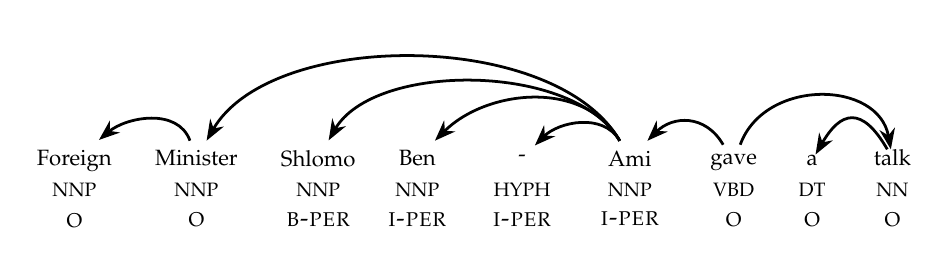
\begin{tikzpicture}[node distance=2.0mm and 5.0mm, >=Stealth, 	place/.style={draw=none, inner sep=0pt}]
		\node [](anode) [] {\footnotesize Foreign};
		\node [](bnode) [right=of anode, xshift=-2mm, yshift=0.28mm] {\footnotesize Minister};
		\node [](cnode) [right=of bnode, xshift=-2mm] {\footnotesize Shlomo};
		\node [](dnode) [right=of cnode, xshift=-2mm] {\footnotesize Ben};
		\node [](enode) [right=of dnode, xshift=3mm] {\footnotesize -};
		\node [](fnode) [right=of enode, xshift=3mm] {\footnotesize Ami};
		\node [](gnode) [right=of fnode, yshift=-0.57mm] {\footnotesize gave};
		\node [place](hnode) [right=of gnode, yshift=0.3mm] {\footnotesize a};
		\node [place](inode) [right=of hnode, yshift=0.3mm, xshift=2mm] {\footnotesize talk};
		
		\node [](at) [below=of anode,yshift=3.0mm]{\scriptsize NNP};
		\node [](bt) [below=of bnode,yshift=2.39mm] {\scriptsize NNP};
		\node [](ct) [below=of cnode,yshift=2.39mm] {\scriptsize NNP};
		\node [](dt) [below=of dnode,yshift=2.39mm]{\scriptsize NNP};
		\node [](et) [below=of enode,yshift=1.7mm]{\scriptsize HYPH};
		\node [](ft) [below=of fnode,yshift=2.39mm]{\scriptsize NNP};
		\node [](gt) [below=of gnode,yshift=2.95mm]{\scriptsize VBD};
		\node [place](ht) [below=of hnode]{\scriptsize DT};
		\node [place](it) [below=of inode,yshift=0.05mm]{\scriptsize NN};
		
		\node [](ae) [below=of at,yshift=2.45mm]{\small \textsc{o}};
		\node [](be) [below=of bt,yshift=2.5mm] {\small \textsc{o}};
		\node [](ce) [below=of ct,yshift=2.5mm] {\small \textsc{b-per}};
		\node [](de) [below=of dt,yshift=2.5mm]{\small \textsc{i-per}};
		\node [](ee) [below=of et,yshift=2.5mm]{\small \textsc{i-per}};
		\node [](fe) [below=of ft,yshift=2.5mm]{\small \textsc{i-per}};
		\node [](ge) [below=of gt,yshift=2.5mm]{\small \textsc{o}};
		\node [place](he) [below=of ht,yshift=0.1mm]{\small \textsc{o}};
		\node [place](ie) [below=of it,yshift=0.1mm]{\small \textsc{o}};
		
		\draw [line width=1pt, -{Stealth[length=3.5mm, open]},->] (bnode) to [out=110,in=40, looseness=1] node [above] {} (anode);
		\draw [line width=1pt, -{Stealth[length=3.5mm, open]},->] (fnode) to [out=120,in=60, looseness=0.8] node [above] {} (bnode);
		\draw [line width=1pt, -{Stealth[length=3.5mm, open]},->] (fnode) to [out=120,in=60, looseness=0.8] node [above] {} (cnode);
		\draw [line width=1pt, -{Stealth[length=3.5mm, open]},->] (fnode) to [out=120,in=45, looseness=1] node [above] {} (dnode);
		\draw [line width=1pt, -{Stealth[length=3.5mm, open]},->] (fnode) to [out=120,in=45, looseness=1] node [above] {} (enode);
		\draw [line width=1pt, -{Stealth[length=3.5mm, open]},->] (gnode) to [out=120,in=45, looseness=1.2] node [above] {} (fnode);
		\draw [line width=1pt, -{Stealth[length=3.5mm, open]},->] (gnode) to [out=70,in=100, looseness=1.2] node [above] {} (inode);
		\draw [line width=1pt, -{Stealth[length=3.5mm, open]},->] (inode) to [out=120,in=60, looseness=1.8] node [above] {} (hnode);
		\end{tikzpicture} 
	\end{subfigure}
	\begin{subfigure}[b]{\linewidth}
		\centering
		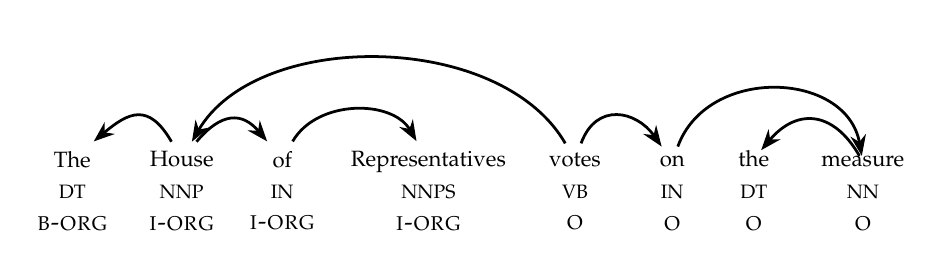
\begin{tikzpicture}[node distance=2.0mm and 5.0mm, >=Stealth, 	place/.style={draw=none, inner sep=0pt}]
		\node [](anode) [] {\footnotesize The};
		\node [](bnode) [right=of anode] {\footnotesize House};
		\node [](cnode) [right=of bnode] {\footnotesize of};
		\node [](dnode) [right=of cnode, yshift=-0.3mm] {\footnotesize Representatives};
		\node [](enode) [right=of dnode, xshift=-2mm, yshift=0.2mm] {\footnotesize votes};
		\node [](fnode) [right=of enode, yshift=-0.2mm] {\footnotesize on};
		\node [place](gnode) [right=of fnode, xshift=0.5mm, yshift=0.35mm] {\footnotesize the};
		\node [place](hnode) [right=of gnode, xshift=1.5mm, yshift=-0.35mm] {\footnotesize measure};
		
		\node [](at) [below=of anode,yshift=2.3mm]{\scriptsize DT};
		\node [](bt) [below=of bnode,yshift=2.3mm] {\scriptsize NNP};
		\node [](ct) [below=of cnode,yshift=2.3mm] {\scriptsize IN};
		\node [](dt) [below=of dnode,yshift=2.9mm]{\scriptsize NNPS};
		\node [](et) [below=of enode,yshift=2.2mm]{\scriptsize VB};
		\node [](ft) [below=of fnode,yshift=2.2mm]{\scriptsize IN};
		\node [place](gt) [below=of gnode, yshift=-0.1mm]{\scriptsize DT};
		\node [place](ht) [below=of hnode, yshift=-0.1mm]{\scriptsize NN};
		
		\node [](ae) [below=of at,yshift=2.25mm]{\small \textsc{b-org}};
		\node [](be) [below=of bt,yshift=2.25mm] {\small \textsc{i-org}};
		\node [](ce) [,below=of ct,yshift=2.3mm] {\small \textsc{i-org}};
		\node [](de) [below=of dt,yshift=2.35mm]{\small \textsc{i-org}};
		\node [](ee) [below=of et,yshift=2.33mm]{\small \textsc{o}};
		\node [](fe) [below=of ft,yshift=2.33mm]{\small \textsc{o}};
		\node [place](ge) [below=of gt, yshift=-0.1mm]{\small \textsc{o}};
		\node [place](he) [below=of ht, yshift=-0.05mm]{\small \textsc{o}};
		
		\draw [line width=1pt, -{Stealth[length=3.5mm, open]},->] (bnode) to [out=120,in=40, looseness=1.5] node [above] {} (anode);
		\draw [line width=1pt, -{Stealth[length=3.5mm, open]},->] (enode) to [out=120,in=60, looseness=0.89] node [above] {} (bnode);
		\draw [line width=1pt, -{Stealth[length=3.5mm, open]},->] (bnode) to [out=50,in=130, looseness=1.4] node [above] {} (cnode);
		\draw [line width=1pt, -{Stealth[length=3.5mm, open]},->] (cnode) to [out=60,in=120, looseness=1] node [above] {} (dnode);
		\draw [line width=1pt, -{Stealth[length=3.5mm, open]},->] (enode) to [out=70,in=125, looseness=1.4] node [above] {} (fnode);
		\draw [line width=1pt, -{Stealth[length=3.5mm, open]},->] (fnode) to [out=70,in=100, looseness=1.2] node [above] {} (hnode);
		\draw [line width=1pt, -{Stealth[length=3.5mm, open]},->] (hnode) to [out=120,in=50, looseness=1.4] node [above] {} (gnode);
		\end{tikzpicture}
	\end{subfigure}
	\caption{Two sentences annotated with both dependency and named entity information. The edges on top of words represent the dependencies and the labels with IOB encoding are the entity types.}
	\label{fig:dgmexample}
\end{figure}


One key observation we can make in Figure \ref{fig:dgmexample} is that named entities are often covered by a single or multiple consecutive dependency arcs.
In the first example, the named entity ``{\em Shlomo Ben - Ami}'' of type \textsc{per} ({\em person}) is completely covered by the single dependency arc from ``{\em Ami}'' to ``{\em Shlomo}''. 
Similarly, the named entity ``{\em The House of Representatives}'' of type \textsc{org} ({\em organization}) in the second example is covered by multiple  arcs which are adjacent to each other. 
Such information can potentially be the global features we can obtain from the dependency trees. 
This leads to the following questions: 1) can such global structured information conveyed by dependency trees be exploited for improved NER, and 2) if so, how to build new NER models where such information can be explicitly incorporated?

With these two questions,  we perform some investigations on how to better utilize the structured information conveyed by dependency trees for building novel models for improved named entity recognition.
The model assumes the availability of dependency trees before performing NER, which can be obtained from a dependency parser or given as part of the input.
Unlike existing approaches that only exploit dependency structures for encoding local features, the model is able to explicitly take into account the global  structured information conveyed by dependency trees when performing learning and inference.
We call our proposed NER model the {\em dependency-guided} model (\textsc{dgm}), and build it based on the conventional semi-Markov conditional random fields (semi-CRFs)~\cite{sarawagi2004semi}, a classic model used for information extraction.

\section{Related Work}
Named entity recognition has a long history in the field of natural language processing. 
One standard approach to NER is to regard the problem as a sequence labeling problem,
where each word is assigned a tag, indicating whether the word belongs to part of any named entity or appears outside of all entities.
Previous approaches used sequence labeling models such as hidden Markov models (HMMs)~\cite{zhou2002named}, maximum entropy Markov models (MEMMs)~\cite{mccallum2000maximum}, as well as linear-chain~\cite{finkel2005incorporating} and semi-Markov conditional random fields (CRFs/semi-CRFs)~\cite{sarawagi2004semi}. 
\citet{muis2016weak} proposed a weak semi-CRFs model which has a lower complexity than the conventional semi-CRFs model while still having a higher complexity than the linear-chain CRFs model. 
Our model is proved to have the same time complexity as linear-chain CRFs model in the average case. 
%To have a better performance, either adding more useful features or exploiting a more complex model is required. 
The quality of the CRFs model typically depends on the features that are used.
While most research efforts exploited standard word-level features~\cite{ratinov2009design}, more sophisticated features can also be used. 
\citet{ling2012fine} showed that using syntactic-level features from dependency structures in a CRFs-based model can lead to improved NER performance.
Such dependency structures were also used in the work by \citet{liu2010recognizing},
where the authors utilized such structures for building a skip-chain variant of the original CRFs model.
This shows that some simple structured information conveyed by dependency trees can be exploited for improved NER. 
%Another more complex models like semi-CRFs \cite{sarawagi2004semi} is known to be generally better than linear-chain CRF though the complexity is higher. 
In their skip-chain CRFs model, they simply added certain dependency arcs as additional dependencies in the graphical model, resulting in loopy structures.
However, such a model did not explicitly explore the relation between entities and global structured information of the dependency trees.
The authors also showed that such a model does not outperform a simpler approach that adds additional dependencies between similar words only on top of the original CRFs model.
%
% they did not consider any entity information given the dependency structure but just simply adding the skip edges to produce more cliques in their graphical model. 
%	Moreover, they need to carefully link such skip edges since it may cause the inference their graphical model intractable. 
In this work, we also focus on utilizing dependency structures for improving NER.
Unlike previous approaches, we focus on exploiting the global structured information conveyed by dependency trees to improve the NER process. Comparing with the semi-CRFs model, our  model is not only able to perform competitively in terms of performance, but also more {\em efficient} in terms of running time.

There are also some existing works that focus on improving the efficiency of NER and other information extraction models.
For example, \citet{okanohara2006improving} used a separate naive Bayes classifier to filter some entities during training and inference in their semi-CRFs based model.
While the filtering process was used to reduce the computational cost of the semi-CRFs model, the model still needs to enumerate all the possible chunks. 
\citet{yang2012extracting} extended the original semi-CRFs for extracting opinion expressions and used the constituency parse tree information to avoid constructing implausible segments. 
\citet{lu2015joint} proposed an efficient and scalable model using hypergraph which can handle overlapping entities. 
\citet{muis2016learning} extended the hypergraph representation to recognize both contiguous and discontiguous entities. 
%-----------------------------------
%	SUBSECTION 1
%-----------------------------------
\section{Background}
Before we introduce our  models, we would like to have a brief discussion on the relevant background. 
Specifically, in this section, we  review the two classic models that are commonly used for named entity recognition, namely the linear-chain conditional random fields and the semi-Markov conditional random fields models.
%In this section, we introduce the conventional linear-chain CRF model as well as the Semi-Markov CRF model for named entity recognition task. We first present the general CRF formalism and then extend it to other variants. Then we propose two Semi-Markov CRF model variants to efficiently complete the NER task though there is a very small amount of cases that cannot fit in our models. 
%Those special cases are fixed by a simple rule which makes the model return to the conventional linear-chain CRF model. 

\subsection{Linear-chain CRFs}
Conditional random fields, or CRFs~\cite{lafferty2001conditional} is a popular model for structured prediction, which has been widely used in various natural language processing problems, including named entity recognition~\cite{mccallum2003early} and semantic role labeling~\cite{cohn2005semantic}. 

We focus our discussions on the linear-chain CRFs in this section.
%In this paper, we also defined a discriminative log-linear model over the dynamic programming derivation.
The probability of predicting a possible output sequence $\vec{y}$ ({\em e.g.}, a named entity label sequence in our case) given an input $\vec{x}$ ({\em e.g.}, a sentence) is defined as:
\begin{equation}
p(\vec{y}|\vec{x}) = \frac{\exp(\vec{\vec{w}^{T}\vec{f}(\vec{x},\vec{y}) })}{Z(\vec{x})}
\end{equation}
where $\vec{f}(\vec{x},\vec{y})$ is the feature vector defined over $(\vec{x},\vec{y})$ tuple, $\vec{w}$ is the weight vector consisting of parameters used for the model, and $Z(\vec{x})$ is the partition function used for normalization, which is defined as follows:
%The optimal output structure is $\vec{y}^{*} = \argmax_{\vec{y}}p(\vec{y}|\vec{x})$. 
%The normalization term $Z(\vec{x})$ represents the score of all the possible structures:
\begin{equation}
Z(\vec{x}) = \sum_{\vec{y}}
\exp
(\vec{w}^{T}\vec{f}(\vec{x}, \vec{y}))
\end{equation}

\begin{figure}[h!]
%	\centering
	\resizebox{0.8\linewidth}{!}{
		\begin{subfigure}[b]{\linewidth}
%			\centering
			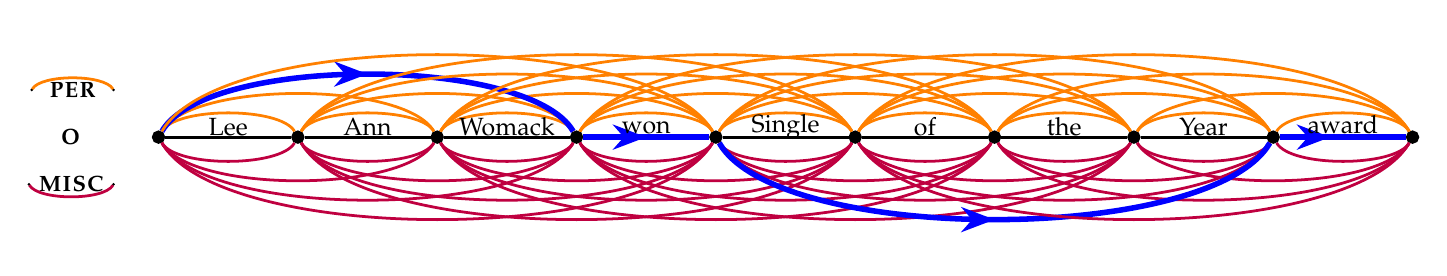
\begin{tikzpicture}[node distance=5mm and 16mm, 
			>=Stealth, inner sep=0mm,
			place/.style={circle, draw, thick, fill=black, inner sep=0.5mm}, smalldot/.style={circle,draw, fill=black,scale=0.5}]			
			\node at (0, 0) [place] (p0){};
			\node [left = of p0, xshift = 9mm, yshift = 6mm](per1) {\textbf{\textsc{per}}};
			\node [left = of per1, xshift = 14mm, smalldot](pr1left) {};
			\node [right = of per1, xshift = -14mm, smalldot](pr1right) {};
			\draw [line width=1pt, -{Stealth[length=3.5mm, open]},-,orange] (pr1left) to [out=60,in=120, looseness=0.55] node [above] {} (pr1right);
			\node [left = of p0, xshift = 7mm, yshift = 0mm](o1) {\textbf{\textsc{o}}};
			\node [left = of p0, xshift = 10mm, yshift = -6mm](misc1) {\textbf{\textsc{misc}}};
			\node [left = of misc1, xshift = 15mm, smalldot](misc1left) {};
			\node [right = of misc1, xshift = -15mm, smalldot](misc1right) {};
			\draw [line width=1pt, -{Stealth[length=3.5mm, open]},-,purple] (misc1left) to [out=-60,in=-120, looseness=0.55] node [above] {} (misc1right);
			\node at (0, 0) [place, right = of p0] (p1){};
			\node at (0, 0) [place, right = of p1] (p2){};
			\node at (0, 0) [place, right = of p2] (p3){};
			\node at (0, 0) [place, right = of p3] (p4){};
			\node at (0, 0) [place, right = of p4] (p5){};
			\node at (0, 0) [place, right = of p5] (p6){};
			\node at (0, 0) [place, right = of p6] (p7){};
			\node at (0, 0) [place, right = of p7] (p8){};
			\node at (0, 0) [place, right = of p8] (p9){};
			
			%% connect the length = 1 entity. PER
			\draw [line width=1pt, -{Stealth[length=3.5mm, open]},-,orange] (p0) to [out=60,in=120, looseness=0.55] node [above] {} (p1);
			\draw [line width=1pt, -{Stealth[length=3.5mm, open]},-,orange] (p1) to [out=60,in=120, looseness=0.55] node [above] {} (p2);
			\draw [line width=1pt, -{Stealth[length=3.5mm, open]},-,orange] (p2) to [out=60,in=120, looseness=0.55] node [above] {} (p3);
			\draw [line width=1pt, -{Stealth[length=3.5mm, open]},-,orange] (p3) to [out=60,in=120, looseness=0.55] node [above] {} (p4);
			\draw [line width=1pt, -{Stealth[length=3.5mm, open]},-,orange] (p4) to [out=60,in=120, looseness=0.55] node [above] {} (p5);
			\draw [line width=1pt, -{Stealth[length=3.5mm, open]},-,orange] (p5) to [out=60,in=120, looseness=0.55] node [above] {} (p6);
			\draw [line width=1pt, -{Stealth[length=3.5mm, open]},-,orange] (p6) to [out=60,in=120, looseness=0.55] node [above] {} (p7);
			\draw [line width=1pt, -{Stealth[length=3.5mm, open]},-,orange] (p7) to [out=60,in=120, looseness=0.55] node [above] {} (p8);
			\draw [line width=1pt, -{Stealth[length=3.5mm, open]},-,orange] (p8) to [out=60,in=120, looseness=0.55] node [above] {} (p9);
			
			%% connect the length = 1 entity. MISC
			\draw [line width=1pt, -{Stealth[length=3.5mm, open]},-,purple] (p0) to [out=-60,in=-120, looseness=0.55] node [above] {} (p1);
			\draw [line width=1pt, -{Stealth[length=3.5mm, open]},-,purple] (p1) to [out=-60,in=-120, looseness=0.55] node [above] {} (p2);
			\draw [line width=1pt, -{Stealth[length=3.5mm, open]},-,purple] (p2) to [out=-60,in=-120, looseness=0.55] node [above] {} (p3);
			\draw [line width=1pt, -{Stealth[length=3.5mm, open]},-,purple] (p3) to [out=-60,in=-120, looseness=0.55] node [above] {} (p4);
			\draw [line width=1pt, -{Stealth[length=3.5mm, open]},-,purple] (p4) to [out=-60,in=-120, looseness=0.55] node [above] {} (p5);
			\draw [line width=1pt, -{Stealth[length=3.5mm, open]},-,purple] (p5) to [out=-60,in=-120, looseness=0.55] node [above] {} (p6);
			\draw [line width=1pt, -{Stealth[length=3.5mm, open]},-,purple] (p6) to [out=-60,in=-120, looseness=0.55] node [above] {} (p7);
			\draw [line width=1pt, -{Stealth[length=3.5mm, open]},-,purple] (p7) to [out=-60,in=-120, looseness=0.55] node [above] {} (p8);
			\draw [line width=1pt, -{Stealth[length=3.5mm, open]},-,purple] (p8) to [out=-60,in=-120, looseness=0.55] node [above] {} (p9);
			
			%% connect the length = 1 entity. O type
			\draw [line width=1pt,-] (p0) to [] node [above] {\small Lee} (p1);
			\draw [line width=1pt,-] (p1) to [] node [above] {\small Ann} (p2);
			\draw [line width=1pt,-] (p2) to [] node [above] {\small Womack} (p3);
			\draw [line width=2pt,->-, blue] (p3) to [] node [above,black] {\small won} (p4);
			\draw [line width=1pt,-] (p4) to [] node [above,yshift=-0.5mm] {\small Single} (p5);
			\draw [line width=1pt,-] (p5) to [] node [above] {\small of} (p6);
			\draw [line width=1pt,-] (p6) to [] node [above] {\small the} (p7);
			\draw [line width=1pt,-] (p7) to [] node [above] {\small Year} (p8);
			\draw [line width=2pt,->--, blue] (p8) to [] node [above,black] {\small award} (p9);
			
			%% connect the length = 2 entity. per 
			\draw [line width=1pt, -{Stealth[length=3.5mm, open]},-,orange] (p0) to [out=60,in=120, looseness=0.55] node [above] {} (p2);
			\draw [line width=1pt, -{Stealth[length=3.5mm, open]},-,orange] (p1) to [out=60,in=120, looseness=0.55] node [above] {} (p3);
			\draw [line width=1pt, -{Stealth[length=3.5mm, open]},-,orange] (p2) to [out=60,in=120, looseness=0.55] node [above] {} (p4);
			\draw [line width=1pt, -{Stealth[length=3.5mm, open]},-,orange] (p3) to [out=60,in=120, looseness=0.55] node [above] {} (p5);
			\draw [line width=1pt, -{Stealth[length=3.5mm, open]},-,orange] (p4) to [out=60,in=120, looseness=0.55] node [above] {} (p6);
			\draw [line width=1pt, -{Stealth[length=3.5mm, open]},-,orange] (p5) to [out=60,in=120, looseness=0.55] node [above] {} (p7);
			\draw [line width=1pt, -{Stealth[length=3.5mm, open]},-,orange] (p6) to [out=60,in=120, looseness=0.55] node [above] {} (p8);
			\draw [line width=1pt, -{Stealth[length=3.5mm, open]},-,orange] (p7) to [out=60,in=120, looseness=0.55] node [above] {} (p9);
			
			%% connect the length = 2 entity. misc
			\draw [line width=1pt, -{Stealth[length=3.5mm, open]},-,purple] (p0) to [out=-60,in=-120, looseness=0.55] node [above] {} (p2);
			\draw [line width=1pt, -{Stealth[length=3.5mm, open]},-,purple] (p1) to [out=-60,in=-120, looseness=0.55] node [above] {} (p3);
			\draw [line width=1pt, -{Stealth[length=3.5mm, open]},-,purple] (p2) to [out=-60,in=-120, looseness=0.55] node [above] {} (p4);
			\draw [line width=1pt, -{Stealth[length=3.5mm, open]},-,purple] (p3) to [out=-60,in=-120, looseness=0.55] node [above] {} (p5);
			\draw [line width=1pt, -{Stealth[length=3.5mm, open]},-,purple] (p4) to [out=-60,in=-120, looseness=0.55] node [above] {} (p6);
			\draw [line width=1pt, -{Stealth[length=3.5mm, open]},-,purple] (p5) to [out=-60,in=-120, looseness=0.55] node [above] {} (p7);
			\draw [line width=1pt, -{Stealth[length=3.5mm, open]},-,purple] (p6) to [out=-60,in=-120, looseness=0.55] node [above] {} (p8);
			\draw [line width=1pt, -{Stealth[length=3.5mm, open]},-,purple] (p7) to [out=-60,in=-120, looseness=0.55] node [above] {} (p9);
			
			%% connect the length = 3 entity. per 
			\draw [line width=2pt, ->-, blue] (p0) to [out=60,in=120, looseness=0.55] node [above] {} (p3);
			\draw [line width=1pt, -{Stealth[length=3.5mm, open]},-,orange] (p1) to [out=60,in=120, looseness=0.55] node [above] {} (p4);
			\draw [line width=1pt, -{Stealth[length=3.5mm, open]},-,orange] (p2) to [out=60,in=120, looseness=0.55] node [above] {} (p5);
			\draw [line width=1pt, -{Stealth[length=3.5mm, open]},-,orange] (p3) to [out=60,in=120, looseness=0.55] node [above] {} (p6);
			\draw [line width=1pt, -{Stealth[length=3.5mm, open]},-,orange] (p4) to [out=60,in=120, looseness=0.55] node [above] {} (p7);
			\draw [line width=1pt, -{Stealth[length=3.5mm, open]},-,orange] (p5) to [out=60,in=120, looseness=0.55] node [above] {} (p8);
			\draw [line width=1pt, -{Stealth[length=3.5mm, open]},-,orange] (p6) to [out=60,in=120, looseness=0.55] node [above] {} (p9);
			
			%% connect the length = 3 entity. misc
			\draw [line width=1pt, -{Stealth[length=3.5mm, open]},-,purple] (p0) to [out=-60,in=-120, looseness=0.55] node [above] {} (p3);
			\draw [line width=1pt, -{Stealth[length=3.5mm, open]},-,purple] (p1) to [out=-60,in=-120, looseness=0.55] node [above] {} (p4);
			\draw [line width=1pt, -{Stealth[length=3.5mm, open]},-,purple] (p2) to [out=-60,in=-120, looseness=0.55] node [above] {} (p5);
			\draw [line width=1pt, -{Stealth[length=3.5mm, open]},-,purple] (p3) to [out=-60,in=-120, looseness=0.55] node [above] {} (p6);
			\draw [line width=1pt, -{Stealth[length=3.5mm, open]},-,purple] (p4) to [out=-60,in=-120, looseness=0.55] node [above] {} (p7);
			\draw [line width=1pt, -{Stealth[length=3.5mm, open]},-,purple] (p5) to [out=-60,in=-120, looseness=0.55] node [above] {} (p8);
			\draw [line width=1pt, -{Stealth[length=3.5mm, open]},-,purple] (p6) to [out=-60,in=-120, looseness=0.55] node [above] {} (p9);
			
			%% connect the length = 4 entity. per 
			\draw [line width=1pt, -{Stealth[length=3.5mm, open]},-,orange] (p0) to [out=60,in=120, looseness=0.55] node [above] {} (p4);
			\draw [line width=1pt, -{Stealth[length=3.5mm, open]},-,orange] (p1) to [out=60,in=120, looseness=0.55] node [above] {} (p5);
			\draw [line width=1pt, -{Stealth[length=3.5mm, open]},-,orange] (p2) to [out=60,in=120, looseness=0.55] node [above] {} (p6);
			\draw [line width=1pt, -{Stealth[length=3.5mm, open]},-,orange] (p3) to [out=60,in=120, looseness=0.55] node [above] {} (p7);
			\draw [line width=1pt, -{Stealth[length=3.5mm, open]},-,orange] (p4) to [out=60,in=120, looseness=0.55] node [above] {} (p8);
			\draw [line width=1pt, -{Stealth[length=3.5mm, open]},-,orange] (p5) to [out=60,in=120, looseness=0.55] node [above] {} (p9);
			
			%% connect the length = 4 entity. misc
			\draw [line width=1pt, -{Stealth[length=3.5mm, open]},-,purple] (p0) to [out=-60,in=-120, looseness=0.55] node [above] {} (p4);
			\draw [line width=1pt, -{Stealth[length=3.5mm, open]},-,purple] (p1) to [out=-60,in=-120, looseness=0.55] node [above] {} (p5);
			\draw [line width=1pt, -{Stealth[length=3.5mm, open]},-,purple] (p2) to [out=-60,in=-120, looseness=0.55] node [above] {} (p6);
			\draw [line width=1pt, -{Stealth[length=3.5mm, open]},-,purple] (p3) to [out=-60,in=-120, looseness=0.55] node [above] {} (p7);
			\draw [line width=2pt, ->-, blue] (p4) to [out=-60,in=-120, looseness=0.55] node [above] {} (p8);
			\draw [line width=1pt, -{Stealth[length=3.5mm, open]},-,purple] (p5) to [out=-60,in=-120, looseness=0.55] node [above] {} (p9);
			\end{tikzpicture}
		\end{subfigure} 
	}
		\resizebox{0.8\linewidth}{!}{
		\begin{subfigure}[b]{\linewidth}
			\centering
			
			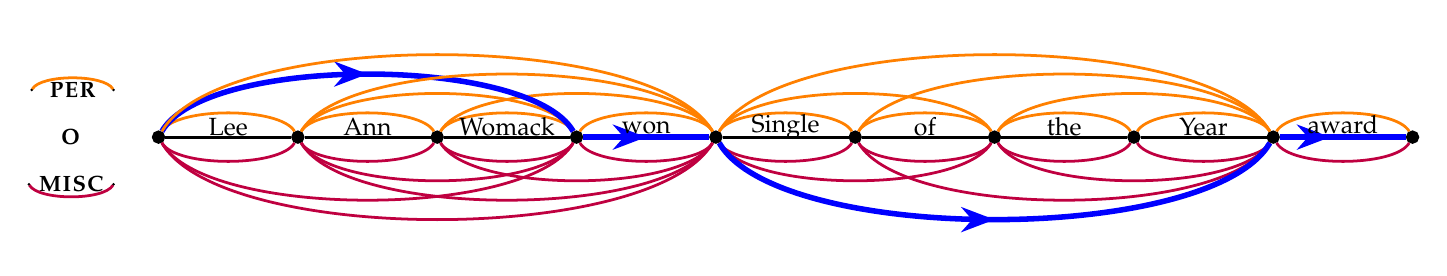
\begin{tikzpicture}[node distance=5mm and 16mm, >=Stealth, inner sep=0mm,
			place/.style={circle, draw, thick, fill=black, inner sep=0.5mm}, smalldot/.style={circle,draw, fill=black,scale=0.5}]
			
			\node at (0, 0) [place] (p0){};
			\node [left = of p0, xshift = 9mm, yshift = 6mm](per1) {\textbf{\textsc{per}}};
			\node [left = of per1, xshift = 14mm, smalldot](pr1left) {};
			\node [right = of per1, xshift = -14mm, smalldot](pr1right) {};
			\draw [line width=1pt, -{Stealth[length=3.5mm, open]},-,orange] (pr1left) to [out=60,in=120, looseness=0.55] node [above] {} (pr1right);
			\node [left = of p0, xshift = 7mm, yshift = 0mm](o1) {\textbf{\textsc{o}}};
			\node [left = of p0, xshift = 10mm, yshift = -6mm](misc1) {\textbf{\textsc{misc}}};
			\node [left = of misc1, xshift = 15mm, smalldot](misc1left) {};
			\node [right = of misc1, xshift = -15mm, smalldot](misc1right) {};
			\draw [line width=1pt, -{Stealth[length=3.5mm, open]},-,purple] (misc1left) to [out=-60,in=-120, looseness=0.55] node [above] {} (misc1right);
			\node at (0, 0) [place, right = of p0] (p1){};
			\node at (0, 0) [place, right = of p1] (p2){};
			\node at (0, 0) [place, right = of p2] (p3){};
			\node at (0, 0) [place, right = of p3] (p4){};
			\node at (0, 0) [place, right = of p4] (p5){};
			\node at (0, 0) [place, right = of p5] (p6){};
			\node at (0, 0) [place, right = of p6] (p7){};
			\node at (0, 0) [place, right = of p7] (p8){};
			\node at (0, 0) [place, right = of p8] (p9){};
			
			%% connect the length = 1 entity. PER
			\draw [line width=1pt, -{Stealth[length=3.5mm, open]},-,orange] (p0) to [out=60,in=120, looseness=0.55] node [above] {} (p1);
			\draw [line width=1pt, -{Stealth[length=3.5mm, open]},-,orange] (p1) to [out=60,in=120, looseness=0.55] node [above] {} (p2);
			\draw [line width=1pt, -{Stealth[length=3.5mm, open]},-,orange] (p2) to [out=60,in=120, looseness=0.55] node [above] {} (p3);
			\draw [line width=1pt, -{Stealth[length=3.5mm, open]},-,orange] (p3) to [out=60,in=120, looseness=0.55] node [above] {} (p4);
			\draw [line width=1pt, -{Stealth[length=3.5mm, open]},-,orange] (p4) to [out=60,in=120, looseness=0.55] node [above] {} (p5);
			\draw [line width=1pt, -{Stealth[length=3.5mm, open]},-,orange] (p5) to [out=60,in=120, looseness=0.55] node [above] {} (p6);
			\draw [line width=1pt, -{Stealth[length=3.5mm, open]},-,orange] (p6) to [out=60,in=120, looseness=0.55] node [above] {} (p7);
			\draw [line width=1pt, -{Stealth[length=3.5mm, open]},-,orange] (p7) to [out=60,in=120, looseness=0.55] node [above] {} (p8);
			\draw [line width=1pt, -{Stealth[length=3.5mm, open]},-,orange] (p8) to [out=60,in=120, looseness=0.55] node [above] {} (p9);
			
			%% connect the length = 1 entity. MISC
			\draw [line width=1pt, -{Stealth[length=3.5mm, open]},-,purple] (p0) to [out=-60,in=-120, looseness=0.55] node [above] {} (p1);
			\draw [line width=1pt, -{Stealth[length=3.5mm, open]},-,purple] (p1) to [out=-60,in=-120, looseness=0.55] node [above] {} (p2);
			\draw [line width=1pt, -{Stealth[length=3.5mm, open]},-,purple] (p2) to [out=-60,in=-120, looseness=0.55] node [above] {} (p3);
			\draw [line width=1pt, -{Stealth[length=3.5mm, open]},-,purple] (p3) to [out=-60,in=-120, looseness=0.55] node [above] {} (p4);
			\draw [line width=1pt, -{Stealth[length=3.5mm, open]},-,purple] (p4) to [out=-60,in=-120, looseness=0.55] node [above] {} (p5);
			\draw [line width=1pt, -{Stealth[length=3.5mm, open]},-,purple] (p5) to [out=-60,in=-120, looseness=0.55] node [above] {} (p6);
			\draw [line width=1pt, -{Stealth[length=3.5mm, open]},-,purple] (p6) to [out=-60,in=-120, looseness=0.55] node [above] {} (p7);
			\draw [line width=1pt, -{Stealth[length=3.5mm, open]},-,purple] (p7) to [out=-60,in=-120, looseness=0.55] node [above] {} (p8);
			\draw [line width=1pt, -{Stealth[length=3.5mm, open]},-,purple] (p8) to [out=-60,in=-120, looseness=0.55] node [above] {} (p9);
			
			%% connect the length = 1 entity. O type
			\draw [line width=1pt,-] (p0) to [] node [above] {\small Lee} (p1);
			\draw [line width=1pt,-] (p1) to [] node [above] {\small Ann} (p2);
			\draw [line width=1pt,-] (p2) to [] node [above] {\small Womack} (p3);
			\draw [line width=2pt,->-,blue] (p3) to [] node [above,black] {\small won} (p4);
			\draw [line width=1pt,-] (p4) to [] node [above, yshift=-0.5mm] {\small Single} (p5);
			\draw [line width=1pt,-] (p5) to [] node [above] {\small of} (p6);
			\draw [line width=1pt,-] (p6) to [] node [above] {\small the} (p7);
			\draw [line width=1pt,-] (p7) to [] node [above] {\small Year} (p8);
			\draw [line width=2pt,->--, blue] (p8) to [] node [above,black] {\small award} (p9);
			
			%% connect the length = 2 entity. per 
			\draw [line width=1pt, -{Stealth[length=3.5mm, open]},-,orange] (p1) to [out=60,in=120, looseness=0.55] node [above] {} (p3);
			\draw [line width=1pt, -{Stealth[length=3.5mm, open]},-,orange] (p2) to [out=60,in=120, looseness=0.55] node [above] {} (p4);
			\draw [line width=1pt, -{Stealth[length=3.5mm, open]},-,orange] (p4) to [out=60,in=120, looseness=0.55] node [above] {} (p6);
			\draw [line width=1pt, -{Stealth[length=3.5mm, open]},-,orange] (p6) to [out=60,in=120, looseness=0.55] node [above] {} (p8);
			
			%% connect the length = 2 entity. misc
			\draw [line width=1pt, -{Stealth[length=3.5mm, open]},-,purple] (p1) to [out=-60,in=-120, looseness=0.55] node [above] {} (p3);
			\draw [line width=1pt, -{Stealth[length=3.5mm, open]},-,purple] (p2) to [out=-60,in=-120, looseness=0.55] node [above] {} (p4);
			\draw [line width=1pt, -{Stealth[length=3.5mm, open]},-,purple] (p4) to [out=-60,in=-120, looseness=0.55] node [above] {} (p6);
			\draw [line width=1pt, -{Stealth[length=3.5mm, open]},-,purple] (p6) to [out=-60,in=-120, looseness=0.55] node [above] {} (p8);
			
			
			%% connect the length = 3 entity. per 
			\draw [line width=2pt, ->-,blue] (p0) to [out=60,in=120, looseness=0.55] node [above] {} (p3);
			\draw [line width=1pt, -{Stealth[length=3.5mm, open]},-,orange] (p1) to [out=60,in=120, looseness=0.55] node [above] {} (p4);
			\draw [line width=1pt, -{Stealth[length=3.5mm, open]},-,orange] (p5) to [out=60,in=120, looseness=0.55] node [above] {} (p8);
			
			
			%% connect the length = 3 entity. misc
			\draw [line width=1pt, -{Stealth[length=3.5mm, open]},-,purple] (p0) to [out=-60,in=-120, looseness=0.55] node [above] {} (p3);
			\draw [line width=1pt, -{Stealth[length=3.5mm, open]},-,purple] (p1) to [out=-60,in=-120, looseness=0.55] node [above] {} (p4);
			\draw [line width=1pt, -{Stealth[length=3.5mm, open]},-,purple] (p5) to [out=-60,in=-120, looseness=0.55] node [above] {} (p8);
			
			
			%% connect the length = 4 entity. per 
			\draw [line width=1pt, -{Stealth[length=3.5mm, open]},-,orange] (p0) to [out=60,in=120, looseness=0.55] node [above] {} (p4);
			\draw [line width=1pt, -{Stealth[length=3.5mm, open]},-,orange] (p4) to [out=60,in=120, looseness=0.55] node [above] {} (p8);
			
			%% connect the length = 4 entity. misc
			\draw [line width=1pt, -{Stealth[length=3.5mm, open]},-,purple] (p0) to [out=-60,in=-120, looseness=0.55] node [above] {} (p4);
			\draw [line width=2pt,->-, blue] (p4) to [out=-60,in=-120, looseness=0.55] node [above] {} (p8);
			
			\end{tikzpicture}
		\end{subfigure}
	}
	\resizebox{0.8\linewidth}{!}{
		\begin{subfigure}[b]{\linewidth}
			\centering
			
			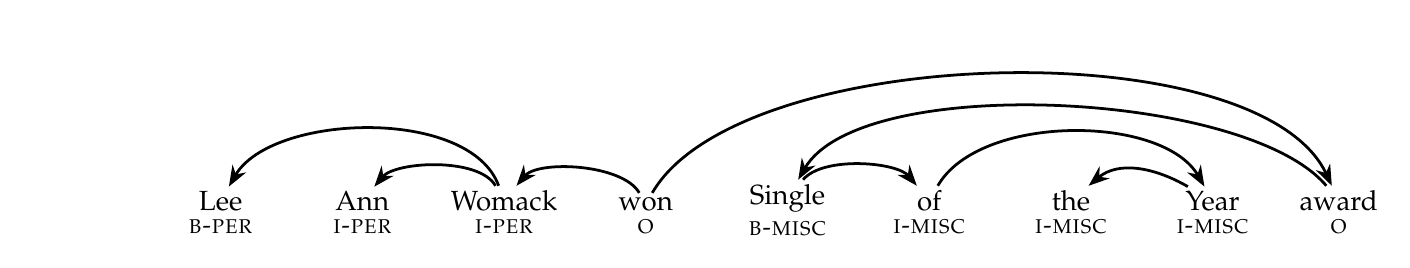
\begin{tikzpicture}[node distance=3mm and 16mm, 
			>=Stealth, inner sep=0.5mm,
			place/.style={circle, draw, thick, fill=black}]
			\node at (0mm, -25mm) [xshift = 0mm, yshift = 8mm](per1) {};
			\node at (24mm, -25mm) [label=below:\small \textsc{b-per},  yshift = -0.05mm] (p0w) {Lee};
			%				\node [left = of p0w, xshift = mm, yshift = 8mm](per1) {sdfsdf};
			\node at (42mm, -25mm) [label=below:\small \textsc{i-per},  yshift = -0.05mm] (p1w) {Ann};
			\node at (60mm, -25mm) [label=below:\small \textsc{i-per}] (p2w) {Womack};
			\node at (78mm, -25.6mm) [label=below:\small \textsc{o},  yshift = 0.15mm] (p3w) {won};
			\node at (96mm, -24.9mm) [label=below:\small \textsc{b-misc},  yshift = 0.2mm] (p4w) {Single};
			\node at (114mm, -25mm) [label=below:\small \textsc{i-misc}] (p5w) {of};
			\node at (132mm, -25mm) [label=below:\small \textsc{i-misc}] (p6w) {the};
			\node at (150mm, -25mm) [label=below:\small \textsc{i-misc},  yshift = -0.05mm] (p7w) {Year};
			\node at (166mm, -25mm) [label=below:\small \textsc{o}] (p8w) {award};
			\draw [line width=1pt, -{Stealth[length=3.5mm, open]},->] (p2w) to [out=110,in=60, looseness=0.8] node [above] {} (p0w);
			\draw [line width=1pt, -{Stealth[length=3.5mm, open]},->] (p2w) to [out=120,in=50, looseness=0.7] node [above] {} (p1w);
			\draw [line width=1pt, -{Stealth[length=3.5mm, open]},->] (p3w) to [out=120,in=50, looseness=0.7] node [above] {} (p2w);
			\draw [line width=1pt, -{Stealth[length=3.5mm, open]},->] (p3w) to [out=60,in=115, looseness=0.65] node [above] {} (p8w);
			\draw [line width=1pt, -{Stealth[length=3.5mm, open]},->] (p4w) to [out=50,in=130, looseness=0.7] node [above] {} (p5w);
			\draw [line width=1pt, -{Stealth[length=3.5mm, open]},->] (p5w) to [out=60,in=120, looseness=0.8] node [above] {} (p7w);
			\draw [line width=1pt, -{Stealth[length=3.5mm, open]},->] (p7w) to [out=150,in=40, looseness=1] node [above] {} (p6w);
			\draw [line width=1pt, -{Stealth[length=3.5mm, open]},->] (p8w) to [out=130,in=60, looseness=0.6] node [above] {} (p4w);
			\end{tikzpicture}
			
		\end{subfigure}
		
		
	}
	\caption{Illustrations of possible combinations of entities for the conventional semi-CRFs model (top) and our \textsc{dgm} model (middle), as well as the example sentence with its dependency structure (bottom).}
	\label{fig:graphexample}
\end{figure}



In a (first-order) linear-chain CRF, the partition function for a input of length $n$ can also be written as follows:
\begin{equation}
Z(\mathbf{x}) = \sum_{\mathbf{y}}\exp\smashoperator{\sum_{(y',y,i)\in\mathcal{E}(\mathbf{x}, \mathbf{y})}}\ \mathbf{w}^T\mathbf{f}(\vec{x}, y',y,i)
\end{equation}
where $\mathcal{E}(\vec{x}, \vec{y})$ is the set of edges which defines the input $\vec{x}$ labeled with the label sequence $\vec{y}$ and $\vec{f}(\vec{x},y', y,i)$ is a local feature vector defined at the $i$-th position of the input sequence.
$T$ is the set of all output labels.
The above function can be computed efficiently using dynamic programming.
It can be seen that the time complexity of a linear-chain CRFs model is $\mathcal{O}(n|T|^{2})$.

We aim to minimize the negative joint log-likelihood with $\textit{L}_{2}$ regularization for our dataset:
%, leading to the following objective function:
\begin{equation}
\begin{split}
\mathcal{L}(\vec{w}) =  \sum_{i}\log\sum_{\substack{\vec{y}{'} } }\exp(\vec{w}^{T}\vec{f}(\vec{x}_{i},\vec{y}{'}))  - \sum_{i}\vec{w}^{T}\vec{f}(\vec{x}_{i},\vec{y}_{i}) + \lambda \vec{w}^{T}\vec{w}
\end{split}
\end{equation} 
where $(\vec{x}_{i},\vec{y}_{i})$ is the $i$-th training instance and $\lambda$ is the $L_{2}$ regularization coefficient.

%The convexity and differentiability of objective function guarantees convergence to the global optimum, and using inside-outside algorithm can efficiently compute the above gradient. There are numbers of techniques can be used for optimizing objective function. 
The objective function is convex and we can make use of the L-BFGS \cite{byrd1995limited} algorithm to optimize it.
The partial derivative of $\mathcal{L}$ with respect to each parameter $w_{k}$ is:
\begin{equation}
%\begin{split}
\frac{\partial\mathcal{L}}{\partial w_{k}}  = \sum_i\Big(\mathbf{E}_{p(\vec{y}{'}|\vec{x}_{i})} \left [f_{k}(\vec{x}_{i}, \vec{y}{'})    \right ] -  f_{k}(\vec{x}_{i}, \vec{y}_{i})\Big) + 2\lambda w_{k}\nonumber
%\end{split}
\end{equation}



\subsection{Semi-Markov CRFs}
The semi-Markov conditional random fields, or semi-CRFs~\cite{sarawagi2004semi} is an extension of the standard linear-chain CRFs.
Different from linear-chain CRFs, which makes use of simple first-order Markovian assumptions, the semi-CRFs
assumes that the transitions between words inside a span ({\em e.g.}, an entity consisting of multiple words) can be non-Markovian.
Such an assumption allows more flexible non-Markovian features to be defined.
The resulting model was shown to be more effective than its linear-chain counterpart in information extraction tasks.
%~\cite{sarawagi2004semi}.

%was first introduced by  in information extraction. 

The partition function in this setting becomes:
%\begin{equation}
%Z(\vec{x}) = \sum_{i=1}^{n} \sum_{l=1}^{L}  \sum_{y'\in T}\sum_{y\in T}\exp(\vec{w}^{T}\vec{f}(\vec{x}, y', y, {i-l}, {i}) )
%\end{equation}
\begin{equation}
Z(\vec{x}) = 
\sum_\vec{y}
\exp \!\!\!\!\! \!\!\!\!\!
\sum_{(y^\prime, y, i-l,i) \in \mathcal{E}(\vec{x}, \vec{y})}
\!\!\!\! \!\!\!\!\!
\vec{w}^{T}\vec{f}(\vec{x}, y^\prime, y, i-l,i)
\end{equation}
where $\vec{f}(\vec{x},y', y, i-l, i)$ represents the local feature vector at position $i$ with a span of size $l$. In this case, the time complexity becomes $\mathcal{O} (nL|T|^{2})$.
The value $L$ is the maximal length of the spans the model can handle.
% depends on the longest entity in training data and the maximum value is the sentence length. 

Consider the sentence ``{\em Lee Ann Womack won Single of the Year award}''.
The upper portion of Figure \ref{fig:graphexample} shows all the possible structures that are considered by the partition function with $L=4$.
These structures essentially form a compact lattice representation showing all the possible combinations of entities (with length restriction)
that can ever appear in the given sentence.
Each orange and red edge is used to represent an entity of type \textsc{per} and \textsc{misc} respectively.
The black lines are used to indicate words that are not part of any entity.
The directed path highlighted in bold blue  corresponds to the correct  entity information associated with the phrase, where ``{\em Lee Ann Womack}'' is an entity of type \textsc{per}, and ``{\em Single of the Year}'' is another entity of  type \textsc{misc} ({\em miscellaneous}).



\section{Our Model}

%We now introduce our model in this section.
The primary assumption we would like to make  is that the dependency trees of sentences are available when performing the  named entity recognition task.
%Such dependency trees can be outputs from some existing dependency parsers.

%We first briefly discuss how to make use of dependency information as features in the NER process, and then discuss how to make use of global structured information of the dependency trees for improved NER.

\subsection{NER with Dependency Features}

One  approach to exploit information from dependency structures is to design local features based on such dependency structures and make use of conventional models such as semi-CRFs for performing NER.
Previous research efforts have shown that such features extracted from dependency structures can be helpful when performing the entity recognition task~\cite{sasano2008japanese,ling2012fine,cucchiarelli2001unsupervised}.

In Figure~\ref{fig:graphexample}, we have already used a graphical illustration to show the possible combinations of entities that can ever appear in the given sentence.
Each edge in the figure corresponds to one entity (or a single word that is outside of any entity -- labeled with \textsc{o}).
%
%
%
%
%the semi-CRFs model for the sentence ``{\em Lee Ann Womack was awarded Single of the Year}''.
%We use different types of nodes to indicate possible semantic classes, and edges are used to indicate boundaries of entities.
%For example, the edge connecting two \textsc{per} nodes indicates an entity  of type \textsc{per} spanning a consecutive sequence of words with boundaries specified by the two end nodes.
%For an edge connecting two different types of nodes, these nodes indicate the left and right boundaries of two entities of different types respectively.
%For example, the edge connecting one \textsc{per} node and one \textsc{misc} node indicates the right boundary of an entity of type \textsc{per} and the left boundary of an entity of type \textsc{misc}.
Features can be defined over such edges, where each feature is assigned a weight.
Such features, together with their weights, can be used to score each possible path in the figure.
%edges connecting different nodes.
When dependency trees are provided, one can define features involving some local dependency structures.
For example, for the word ``{\em Womack}'', one possible feature that can be defined over edges covering this word can be of the form ``{\em Womack }$\leftarrow${\em won}'', indicating there is an incoming arc from the word ``{\em won}'' to the current word ``{\em Womack}''.
However, we note that such features largely ignore the global structured information as presented by the dependency trees.
Specifically, certain useful facts such as the word ``{\em Lee}'' is a child of the word ``{\em Womack}'' and at the same time a grandchild of the word ``{\em won}'' is not captured due to such a simple treatment of dependency structures.

\subsection{Dependency-Guided NER}

%In the upper part of Figure~\ref{fig:graphexample}, \dots

The main question we would like to ask is: how should we make good use of the structured information associated with the dependency trees to perform named entity recognition?
Since we are essentially interested in NER only, would there be some more global structured information in the dependency trees that can be used to guide the NER process?

From the earlier two examples shown in  Figure \ref{fig:dgmexample} as well as the example shown in Figure \ref{fig:graphexample} we can observe that the named entities tend to be covered by a single or multiple adjacent dependency arcs.
This is not a surprising finding as for most named entities which convey certain semantically meaningful information, 
it is expected that there exist certain internal structures -- {\em i.e.}, dependencies amongst different words within the entities.
Words inside each named entity typically do not have dependencies with words outside the entities, except for certain words such as head words which typically have incoming arcs from outside words.

This finding motivates us to exploit such global structured information as presented by dependency trees for performing  NER.
Following the above observation, we first introduce the following notion:
\begin{definition}[Definition 1]
	\label{def:1}
	A {\em valid span} either consists of a single word, or is a word sequence that is covered by a  chain of (undirected) arcs where no arc is covered by another.
\end{definition}

For example, in Figure \ref{fig:graphexample}, the word sequence ``{\em Lee Ann Womack}'' is a valid span since there exists a single arc from ``{\em Womack}'' to ``{\em Lee}''. The sequence ``{\em Ann Womack won}'' is also a valid span due to a chain of undirected arcs -- one between ``{\em Ann}'' and ``{\em Womack}'' and the other between ``{\em Womack}'' and ``{\em won}''.
Similarly, the single word ``{\em Womack}'' is also a valid span given the above definition.

Based on the above definition, we can build a novel dependency-guided NER model based on the conventional semi-CRFs  by restricting the space of all possible combinations of entities to those that strictly contain only valid spans.
This leads to the following new partition function:
\begin{equation}
Z(\vec{x}) = \!\!\!\!\!\!\sum_{(i,j)\in\mathcal{S}_L(\vec{x})}\sum_{y'\in T} \sum_{y\in T}\exp(\vec{w}^{T}\vec{f}(\vec{x}, y', y, {i}, {j}) )
\end{equation}
where $\mathcal{S}(\mathbf{x})$ refers to the set of valid spans for a given input sentence $\mathbf{x}$, and $\mathcal{S}_L(\mathbf{x})$ refers to its subset that contains only those valid spans whose lengths are no longer than $L$.

We call the resulting model {\em dependency-guided model} (\textsc{dgm}).
Figure \ref{fig:graphexample} (middle) presents the graphical illustration of all possible paths (combination of entities) with $L=4$ that our model considers.
For example, since the word sequence ``{\em Ann Womack won Single}'' is not a valid span, the corresponding edges covering this word sequence is removed from the original lattice representation in Figure \ref{fig:graphexample} (top).
The edge covering the word sequence ``{\em of the Year}'' remains there as it is covered by the arc from ``{\em of}'' to ``{\em Year}'', thus a valid span.
As we can see, the amount of paths that we consider in the new model is substantially reduced.

\subsection{Time Complexity}
We can also analyze the time complexity required for this new model. We show example best-case and worst-case scenarios in Figure~\ref{fig:scenarios_analysis}.
For the former case there are $\mathcal{O} (n)$ valid spans. Thus the time complexity in the best case is $\mathcal{O} (n|T|^2)$, the same as the linear-chain CRFs model.
For the latter, there are $\mathcal{O} (nL)$ valid spans, leading to the time complexity $\mathcal{O} (nL|T|^2)$ in the worst case, the same as the semi-Markov CRFs model.
%This analysis shows the potential of our model -- empirically it can run faster than the conventional semi-Markov CRFs model.
%We will confirm this later through empirical analysis.

\begin{figure}[t!]
%	\small
	%	\centering
	\begin{subfigure}[t]{0.51\linewidth}
		\centering
		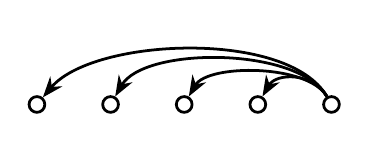
\begin{tikzpicture}[node distance=3mm and 7mm, >=Stealth]
		\node[place,line width=1pt, minimum size=0.2cm] (p1) {};
		\node[place,line width=1pt, right=of p1, minimum size=0.2cm] (p2) {};
		\node[place,line width=1pt, right=of p2, minimum size=0.2cm] (p3) {};
		\node[place,line width=1pt, right=of p3, minimum size=0.2cm] (p4) {};
		\node[place,line width=1pt, right=of p4, minimum size=0.2cm] (p5) {};
		\draw [line width=1pt, -{Stealth[length=3.5mm, open]},->] (p5) to [out=120,in=50, looseness=0.7] node [above] {} (p1);
		\draw [line width=1pt, -{Stealth[length=3.5mm, open]},->] (p5) to [out=120,in=60, looseness=0.7] node [above] {} (p2);
		\draw [line width=1pt, -{Stealth[length=3.5mm, open]},->] (p5) to [out=120,in=60, looseness=0.7] node [above] {} (p3);
		\draw [line width=1pt, -{Stealth[length=3.5mm, open]},->] (p5) to [out=120,in=60, looseness=1.1] node [above] {} (p4);
		\end{tikzpicture}
		\caption{Best-case Scenario}
		\label{fig:bestcase} 
	\end{subfigure}
	\begin{subfigure}[t]{0.48\linewidth}
		\centering
		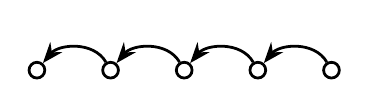
\begin{tikzpicture}[node distance=3mm and 7mm, >=Stealth]
		\node[place,line width=1pt, minimum size=0.2cm] (p1) {};
		\node[place,line width=1pt, right=of p1, minimum size=0.2cm] (p2) {};
		\node[place,line width=1pt, right=of p2, minimum size=0.2cm] (p3) {};
		\node[place,line width=1pt, right=of p3, minimum size=0.2cm] (p4) {};
		\node[place,line width=1pt, right=of p4, minimum size=0.2cm] (p5) {};
		\draw [line width=1pt, -{Stealth[length=3.5mm, open]},->] (p5) to [out=120,in=50, looseness=1] node [above] {} (p4);
		\draw [line width=1pt, -{Stealth[length=3.5mm, open]},->] (p4) to [out=120,in=50, looseness=1] node [above] {} (p3);
		\draw [line width=1pt, -{Stealth[length=3.5mm, open]},->] (p3) to [out=120,in=50, looseness=1] node [above] {} (p2);
		\draw [line width=1pt, -{Stealth[length=3.5mm, open]},->] (p2) to [out=120,in=50, looseness=1] node [above] {} (p1);
		\end{tikzpicture}
		\caption{Worst-case Scenario}
		\label{fig:worstcase} 
	\end{subfigure}
	\caption{The best-case and worst-case scenarios of  \textsc{dgm}.}
	\label{fig:scenarios_analysis}
\end{figure}

Furthermore, we have the following theorem for the average-case time complexity:
\begin{theorem}
	The average-case time complexity of \textsc{dgm} is $\mathcal{O}(n|T|^2)$.
\end{theorem}
\begin{proof}
	
	We refer the readers to our full paper~\cite{jie2017efficient} with appendix\footnote{https://arxiv.org/pdf/1810.08436.pdf}.
	We credit Aldrian with his substantial effort for the complexity derivation.
\end{proof}

%(We provide a detailed proof in the following section \ref{sec:numedges})
%We provide the detailed proof in our full paper~\cite{jie2017efficient} with appendix\footnote{https://arxiv.org/pdf/1810.08436.pdf}.

Now, this is a remarkable result, showing that the  complexity of our \textsc{dgm} model in its average case is still linear in the sentence length $n$ even if we set $L$ to its maximal value $n$. This is also true empirically, which we show in the supplementary material (S.3.2).
% is independent of $L$ ({\em i.e.}, one can set the value of $L$ to up to $n$).
So, while our model retains the ability to capture non-Markovian features like semi-Markov CRFs,
it is more scalable and can be used to extract longer entities.

%\begin{theorem}
%	For the inference algorithm of \textsc{dgm}, its best-case time complexity  is in $\mathcal{O}(n|T|)$, and the worst-case is in $\mathcal{O}(nL|T|^2)$.
%\end{theorem}
%
%\begin{proof}[Proof Sketch]
%	The best-case and worst-case scenarios are illustrated in Figure \ref{fig:scenarios_analysis}.
%	We can see that for the best-case scenario, for each entity type there are $(n-1)$ possible spans.
%\end{proof}

%In the conventional Semi-Markov Model setting, the normalization term becomes:
%\begin{equation}
%Z(\vec{x}) = \sum_{i=1}^{n} \sum_{y_{i}\in T}\sum_{l=1}^{L} \sum_{y_{i-l}\in T}\exp(\vec{w}^{T}\vec{f}(\vec{x},y_{i-l}, y_{i}) )
%\end{equation}
%where $\vec{f}(\vec{x},y_{i-l}, y_{i})$ represents the feature vector on the edges that connecting label $y_{i}$ and label $y_{i-k}$. In this case, the time complexity should be $\mathcal{O} (nL|T|^{2})$. The $L$ depends on the longest entity in training data and the maximum value is the sentence length. 

%\subsection{Dependency-based Segment Model (DSM)}
%In our first model, we consider to remove most of the edges while building the model based on the relationship between the dependency and named entity. 
%
%Take Figure \ref{fig:graphexample} as an example, some of the edges can be removed if we already have the dependency information. 
%In this case, we still have the full connections at all adjacent positions. Thus, the complexity of Linear-chain CRF is still there.
%Then the segment connections between non-adjacent positions depend on the number of dependencies. Under a dependency arc, we also have the fully connections between all the labels at non-adjacent positions except for the $O$ label since the $O$ label is always considered as a segment with length 1 \cite{sarawagi2004semi}. That means we have $\mathcal{O}(|T|^{2})$ connections for each dependency and there are in $\mathcal{O}(n)$ dependencies in total. The normalization term becomes:
%\begin{align}
%\begin{split}
%Z(\vec{x}) &  = \sum_{i=1}^{n} \sum_{y_{i-1}\in T} \sum_{y_{i}\in T}\exp(\vec{w}^{T}\vec{f}(\vec{x},y_{i-1}, y_{i}) )\\
%& + \sum_{i=1}^{n} \sum_{y_{i}\in T}\sum_{y_{ih}\in T}\exp(\vec{w}^{T}\vec{f}(\vec{x},y_{ih}, y_{i}) )
%\end{split}
%\end{align}
%where $y_{i\_dep}$ represents the head label of the current position $i$. The time complexity is still $\mathcal{O} (n|T|^{2})$. As in the first observation, there are about 94\% of entities can be handled this model. 

%\subsection{Extra-Dependency-based Segment Model (EDSM)}
%Model 1 can deal with about 96\% of all the entities, but there are rooms to improve the model. So based on the second observation, we build another Semi-Markov model that can handle more than 99\% of all the entities that in the form of figure \ref{fig:twoexample}.  
%
%Specifically, take figure \ref{fig:model2example} as an example, there are no dependency arc cover the whole entity \textsc{Telerate} \textsc{Systems} \textit{Inc} now. Now we look at a window within the entity only, all the dependencies outside this window are removed. Thus, the structure becomes something like:
%\begin{figure}[h]
%	\centering
%	\begin{tikzpicture}[node distance=3.5mm and 3.5mm, >=Stealth]
%	\node [](c_node) [] {Voice};
%	\node [](d_node) [ right=of c_node] {of};
%	\node [](e_node) [right=of d_node] {America};
%	
%	\node [](ct_node) [label=below:\small \textsc{b-org},below=of c_node,yshift=5mm] {\scriptsize NNP};
%	\node [](dt_node) [label=below:\small \textsc{i-org},below=of d_node,yshift=5mm]{\scriptsize NNP};
%	\node [](et_node) [label=below:\small \textsc{i-org},below=of e_node,yshift=5mm]{\scriptsize NNP};
%	
%	\draw [line width=1pt, -{Stealth[length=3.5mm, open]}, ->] (c_node) to [out=60,in=120, looseness=1] node [above] {} (d_node);
%	\draw [line width=1pt, -{Stealth[length=3.5mm, open]}, ->] (d_node) to [out=60,in=120, looseness=1] node [above] {} (e_node);
%	\end{tikzpicture}
%	\caption{The representation after we crop a ``window'' from sentence}
%	\label{fig:model2example}
%\end{figure}


%We further make the dependencies in this window become undirected links. It's obvious to see that all these links make the entity connected. Inspired by this observation, we can build another somewhat complex model to handle these cases. The idea in our graphical representation is to connect the partial entity given the previous connection and then the whole entity will become a segment after this process. To make it clear, figure \ref{fig:threestep} shows the process of building such model. 

%As the previous model, the complexity of the linear-chain CRF still exist in our model 2. The normalization term in this case becomes:
%\begin{align*}
%\begin{split}
%Z(\vec{x}) &  = \sum_{i=1}^{n} \sum_{y_{i-1}\in T} \sum_{y_{i}\in T}\exp(\vec{w}^{T}\vec{f}(\vec{x},y_{i-1}, y_{i}) )\\
%& + \sum_{i=1}^{n} \sum_{y_{i}\in T}\sum_{\substack{y_{ih}\in T \\ y_{i}\neq y_{ih}}}\exp(\vec{w}^{T}\vec{f}(\vec{x},y_{ih}, y_{i}) ) \\
%& + \sum_{i=1}^{n} \sum_{y_{i}\in T}\sum_{\substack{\text{child}(y_{ih}) \\  y_{ih}=y_{i}} }\exp(\vec{w}^{T}\vec{f}(\vec{x},\text{child}(y_{ih}), y_{i}) ) \\
%\end{split}
%\end{align*}
%
%Overall, the complexity in our model 2 depends on the number of children that a node has. The complexity can be equal to original Semi-Markov CRF model. But in practice, the decoding time is faster than the original Semi-Markov CRF model. 
%%%Make a proof to prove that it's still more efficient then orignial semimarkov
%Thus, using our model 2 still has a lower complexity than the original semi-Markov CRF model. Though many edges are removed in our model, the dependency information is essentially implicitly embedded in the Semi-Markov model. 
%


%\begin{figure*}[h]
%	\centering
%	\subfigure[First Step]{\label{fig:dfdf} 
%		\includegraphics[width=1.8in]{imgs/firststep.pdf}
%	} \hfill
%	\subfigure[Second Step]{\label{fig:dfdf} 
%		\includegraphics[width=1.8in]{imgs/secondstep.pdf}
%	} \hfill
%	\subfigure[Third Step]{\label{fig:dfdf} 
%		\includegraphics[width=1.8in]{imgs/thirdstep.pdf}
%	}
%	\caption{The three-step graphical model construction based on the example in figure \ref{fig:model2example}. (a) When we construct the connections of \textsc{org} in the middle position, all the nodes in previous position are connected based on the dependency from \textit{Systems} to \textit{Telerate}. (b) when we see the second dependency from \textit{Systems} to \textit{Inc}, we also connect all the nodes in previous positions except the link between \textsc{org} and \textsc{org}. (c) Thus when we see the nodes with same types, we connect to all its children instead of the previous node.}
%	\label{fig:threestep}
%\end{figure*}

%\subsection{Special Cases}
%There are some other special cases (about 0.06\%) that still cannot even be handled by EDSM since they are not really ``connected'' by the definition in EDSM. For example in figure \ref{fig:specialcase}, the \textsc{misc} entity , \textit{Hasidic Jewish}, has a head from \textit{family}. Thus, if we look at the entity window and remove all the dependencies from this window, all the two words in this entity are isolated. Since the portion of this kind of structure is very small, we use the linear-chain structure to connect this two words when we encounter this case during training. 
% 
%\begin{figure}[h]
%	\centering
%	\begin{tikzpicture}[node distance=2.9mm and 2.9mm, >=Stealth]
%		\node [](a_node) [] {Hasidic};
%		\node [](b_node) [right=of a_node] {Jewish} ;
%		\node [](c_node) [right=of b_node] {family};
%		
%		\node [](at_node) [label=below:\small \textsc{b-misc},below=of a_node,yshift=4mm]{\scriptsize JJ};
%		\node [](bt_node) [label=below:\small \textsc{i-misc} ,below=of b_node,yshift=4mm]{\scriptsize JJ};
%		\node [](ct_node) [label=below:\small \textsc{o},below=of c_node,yshift=4mm] 	{\scriptsize NN};
%
%		
%		\draw [line width=1pt, -{Stealth[length=3.5mm, open]}, <-] (a_node) to [out=60,in=110, looseness=1] node [above] {} (c_node);
%		\draw [line width=1pt, -{Stealth[length=3.5mm, open]}, <-] (b_node) to [out=60,in=130, looseness=1] node [above] {} (c_node);
%		
%	\end{tikzpicture}
%	\caption{Special case: the entity that is not ``connected'' by the dependencies}
%	\label{fig:specialcase}
%\end{figure}


%\subsection{Model Refinement}
%Though there is a strong relationship between dependency and the named entity, some other dependencies are still not useful for the model. For the short dependency, we might not sure whether it is covering an entity or not. Thus, we then turn to focus on eliminating some long dependencies. We can limit the maximum length of the entity and ignore those dependencies whose length is larger than this maximum length value.
%% Connect to the same type or not?
%%remove the edges.{}

Besides the standard \textsc{dgm} model defined above, we also consider a variant, where we restrict the  chain (of arcs) to be of length 1 ({\em i.e.}, single arc) only. We call the resulting model \textsc{dgm-s}, where \textsc{s} stands for {\em single arc}.
Such a simplified model will lead to an even simpler lattice representation, resulting in even less running time.
However it may also lead to  lower performance as such a  variant might not be able to capture certain named entities.
In one of the later sections, we will conduct experiments on such a model and compare its performance with other models.

\subsection{Number of Edges}
\label{sec:numedges}
The number of edges in a graphical model is proportional to the time complexity of training the model, and so in the interest of calculating the time complexity of the models, in this section we show theoretically that on average case, the number of edges in our \textsc{dgm} model is linear in terms of $n$, the number of words in a sentence. Then for all models we show empirically the relationship between the number of edges and the sentence length $n$.

%\subsubsection{Theoretical Analysis}
%In this section we show how to calculate the average number of edges in the \textsc{dgm} model for a sentence of length $n$. Note that the number of edges in the model is by definition equal to the number of valid spans, as an edge is added in the model connecting the beginning of the first word and the end of the last word of each valid span. In the first analysis, we will count the valid spans that cover more than one words separately from the valid spans covering only one word. Since the valid spans covering one word are always present, the count is known, there are $n$ of them for each graph in the model. So in the first method we count only the valid spans covering more than one words.
%
%We first calculate the total number of edges in the \textsc{dgm} model over all possible undirected trees, then the average is just this number divided by the number of undirected trees. 
%Although dependency trees are directed trees, calculating the average on undirected trees is sufficient as for each undirected tree there is exactly $n$ possible dependency trees, one for each selection of node as the root of the tree, and so the average number of edges will be the same. Note that we consider both projective and non-projective trees here. Later the empirical count will provide an evidence that the average number of edges calculated here still holds even in a dataset where most of the trees are projective.
%
%More formally, if the vertex set for the graph $G_{\tau}$ in the \textsc{dgm} model with the undirected dependency tree $\tau$ is $V(G_{\tau}) = \{1,2,\ldots,n\}$ and the edge set of the tree is $E(\tau)$, then the edge set of the graph in the model is $E_{\textsc{dgm}}(G_{\tau}) = \{(u_1,u_{k+1})\ |\ \exists\ u_1<u_2<\ldots<u_{k+1}\ \text{s.t.}\ (u_i,u_{i+1})\in E(\tau),\ \forall i=1,2,\ldots,k,\ k\geq 1\}$. We present two alternative methods to count the average, the first using algebra, and the second using bijection. Although the first method is more complicated, along the process it also calculates the relationship between the average number of edges and $L$, the maximum valid span length. In this supplementary material, we present only the first method. The proof by bijection is already covered in the main paper~\cite{jie2017efficient}.
%
%\subsubsection{Proof by Algebra}
%
%To count the number of edges over all possible trees, we consider each pair of nodes $u$ and $v$ in the graph, where $u<v$. Let $f_n(u,v)$ be the number of times there is an edge in the \textsc{dgm} model, over all possible trees. More formally, the number of times $f_n(u,v)$ can be computed as $f_n(u,v) = \sum_{\tau\in\mathcal{T}(n)} I\left[(u,v)\in E_{\textsc{dgm}}(G_{\tau})\right]$, where $I[F]$ is the indicator function, which is $1$ if the expression $F$ is true, $0$ otherwise, and $\mathcal{T}(n)$ is the set of all possible trees with $n$ nodes. Also, let $F(n, L)$ as the total number of edges in \textsc{dgm} model where the maximum valid span length is $L$. We are looking for $\bar{F}(n,n)$, the average number of edges in \textsc{dgm} in all possible trees when $L$ is not restricted.
%
%First, to calculate $f_n(u,v)$, we consider the number of intermediate nodes between $u$ and $v$. Note that, by definition of the $E_{\textsc{dgm}}(G_{\tau})$, the intermediate nodes must appear between $u$ and $v$, and for any set of intermediate nodes there is exactly one set of edges that leads to $(u,v)$ being a valid span, that is when there is no edge covered by another. If $k$ is the number of intermediate nodes, then there are $\binom{v-u-1}{k}$ ways to choose the path from $u$ to $v$, and we can multiply this by the number of trees that contain each path to get $f_n(u,v)$. Note that for a path with $k$ intermediate nodes, there are $k+2$ nodes, including $u$ and $v$, among the $n$ nodes which are already connected. If we remove these edges from the tree that contains the path, we will be left with a forest with $k+2$ components, as each of the $k+2$ nodes will be disconnected from each other, due to the property of trees that there is a unique path between any two nodes. So the number of trees that contain a path with $k+2$ nodes is equal to the number of forest with $n$ nodes and $k+2$ components, which is well-established as $(k+2)n^{n-k-3}$ (see, for example \cite[Chapter 30]{Aigner2010}).
%
%So we have:
%\begin{eqnarray}
%f_n(u,v) &=& \sum_{k=0}^{v-u-1}\binom{v-u-1}{k}(k+2)n^{n-k-3}\nonumber\\
%&=& \sum_{k=0}^{v-u-1}\binom{v-u-1}{v-u-1-k}(v-u-1-k+2)n^{n-(v-u-1-k)-3}\nonumber\\
%&=& n^{n-v+u-2}\sum_{k=0}^{v-u-1}\binom{v-u-1}{k}(v-u+1-k)n^k\nonumber\\
%&=& n^{n-v+u-2}\left[(v-u+1)\sum_{k=0}^{v-u-1}\binom{v-u-1}{k}n^k - \sum_{k=0}^{v-u-1}\binom{v-u-1}{k}kn^k\right]\nonumber\\
%&=& n^{n-3-(v-u-1)}\left[(v-u+1)(n+1)^{v-u-1} - n(v-u-1)(n+1)^{v-u-2}\right]\nonumber\\
%&=& n^{n-3}\left[(v-u+1)\left(1+\frac{1}{n}\right)^{v-u-1} - (v-u-1)\left(1+\frac{1}{n}\right)^{v-u-2}\right]\nonumber\\
%&=& n^{n-3}\left[\left(v-u+1 - \frac{n(v-u-1)}{n+1}\right)\left(1+\frac{1}{n}\right)^{v-u-1}\right]\nonumber\\
%&=& n^{n-3}\left(\frac{2n+1+v-u}{n+1}\right)\left(1+\frac{1}{n}\right)^{v-u-1}\nonumber
%\end{eqnarray}
%
%To get from (1) to (2) we used the expansion of binomial formula and its derivative, as follows:
%\begin{align*}
%\qquad\qquad\qquad\qquad\qquad\qquad&&(x+1)^n &= \sum_{k=0}^n\binom{n}{k}x^k&&\nonumber\\
%\qquad\qquad\qquad\qquad\qquad\qquad&&n(x+1)^{n-1} &= \sum_{k=0}^n\binom{n}{k}kx^{k-1}&&\text{(take derivative both sides)}\nonumber\\
%\qquad\qquad\qquad\qquad\qquad\qquad&&nx(x+1)^{n-1} &= \sum_{k=0}^n\binom{n}{k}kx^k&&\text{(multiply by $x$)}\nonumber
%\end{align*}
%\noindent with $n$ and $x$ substituted for $v-u-1$ and $n$ respectively to get from (1) to (2). Note that since the formula depends on $u$ and $v$ only from the difference $v-u$, let us define $f_n(k) = f_n(u, u+k)$.
%
%Now, the number of total edges is the sum of $f_n(u,v)$ over all possible values for $u$ and $v$, yielding our final formula for $F(n, L)$, the total number of edges when the maximum valid span is of length $L$:
%\begin{eqnarray}
%F(n,L) \!\!&=& \sum_{u=1}^{n-1}\sum_{v=u+1}^{u+L-1} f_n(u,v)\nonumber\\
%&=& \sum_{k=1}^{L-1}\sum_{u=1}^{n-k} f_n(k)\nonumber\\
%&=& \sum_{k=1}^{L-1}(n-k)n^{n-3}\left(\frac{2n+1+k}{n+1}\right)\left(1+\frac{1}{n}\right)^{k-1}\nonumber\\
%&=& \frac{n^{n-3}}{n+1}\sum_{k=1}^{L-1}(n-1-(k-1))(2n+2+(k-1))\left(1+\frac{1}{n}\right)^{k-1}\nonumber\\
%&=& \frac{n^{n-3}}{n+1}\sum_{k=0}^{L-2}(n-1-k)(2n+2+k)\left(1+\frac{1}{n}\right)^k\nonumber\\
%&=& \frac{n^{n-3}}{n+1}\left[(n-1)(2n+2)\sum_{k=0}^{L-2}\left(1+\frac{1}{n}\right)^k - (n+3)\sum_{k=0}^{L-2}k\left(1+\frac{1}{n}\right)^k - \sum_{k=0}^{L-2}k^2\left(1+\frac{1}{n}\right)^k\right]\ \ \ \ \nonumber\\
%&=& \frac{n^{n-3}}{n+1}\left[(n-1)(2n+2)n\left(\left(1+\frac{1}{n}\right)^{L-1}-1\right)\right.\nonumber\\
%&& -(n+3)\left(n(L-1)\left(1+\frac{1}{n}\right)^{L-1}-n^2\left(1+\frac{1}{n}\right)^{L}+n^2\left(1+\frac{1}{n}\right)\right)\nonumber\\
%&& \left.-(n(L-2)^2-2n^2(L-2)+2n^3+n^2)\left(1+\frac{1}{n}\right)^{L-1}+n^3\left(1+\frac{1}{n}\right)^2+n^3\left(1+\frac{1}{n}\right)\right]\nonumber\\
%&=& \frac{n^{n-3}}{n+1}\left[n(n^2+L(n-L+1))\left(1+\frac{1}{n}\right)^{L-1}-n^2(n+1)\right]\nonumber\\
%&=& \frac{n^{n-2}}{n+1}\left[(n^2+L(n-L+1))\left(1+\frac{1}{n}\right)^{L-1}-n(n+1)\right]\nonumber
%\end{eqnarray}
%\noindent which, when $L = n$, that is when we do not restrict the valid span length, we have:
%\begin{eqnarray}
%F(n, n) &=& n^{n-1}\left[\left(1+\frac{1}{n}\right)^{n-1}-1\right] = (n+1)^{n-1} - n^{n-1}\nonumber
%\end{eqnarray}
%
%We used geometric sums formula and its derivatives (equations (5), (6), and (7)) to get from (3) to (4):
%\begin{eqnarray}
%\frac{x^{n+1}-1}{x-1} \!\!&=&\!\! \sum_{k=0}^n x^k\nonumber\\
%\frac{(n+1)x^{n+1}(x-1) - x(x^{n+1}-1)}{(x-1)^2} \!\!&=&\!\! \sum_{k=0}^n kx^k\nonumber\\
%\frac{nx^{n+2}-(n+1)x^{n+1}+x}{(x-1)^2} \!\!&=&\!\! \sum_{k=0}^n kx^k\nonumber\\
%x\frac{(n(n+2)x^{n+1}-(n+1)^2x^n+1)(x-1)^2 - 2(nx^{n+2}-(n+1)x^{n+1}+x)(x-1)}{(x-1)^4} \!\!&=&\!\! \sum_{k=0}^n k^2x^k\nonumber\\
%x\frac{(n(x-1)(n(x-1)-2)+x+1)x^n-x-1}{(x-1)^3} \!\!&=&\!\! \sum_{k=0}^n k^2x^k\quad\nonumber
%\end{eqnarray}
%
%Finally, the average of number of edges is $F(n, n)$, plus the number of valid spans covering one word, which is $n\cdot{}n^{n-2}$, divided by total number of trees, which is $T(n,1) = n^{n-2}$, which yields the average:
%
%\begin{eqnarray}
%\bar{F}(n) &=& \frac{((n+1)^{n-1}-n^{n-1}) + n^{n-1}}{n^{n-2}}\nonumber\\
%&=& n\left(1+\frac{1}{n}\right)^{n-1}\nonumber\\
%&\leq& \mathbf{e}n\nonumber
%\end{eqnarray}
%\noindent where $\mathbf{e}$ is the Euler's number, which is approximately 2.718.
%
%So we can see that on average, the number of edges present in the \textsc{dgm} model for one entity type is linear in terms of $n$, the number of words in the sentence. When there are $\left\lvert T\right\rvert$ types, the number of edges will be multiplied by $\left\lvert T\right\rvert^2$ since for each edge there are $\left\lvert T\right\rvert^2$ possible type combination for the start and end of the span. {\bf Therefore the time complexity of the training process of \textsc{dgm} model when there are $\left\lvert T\right\rvert$ types is $\mathcal{O}(n\left\lvert T\right\rvert^2)$.}
%
%%\subsubsection{Second Method: Bijection}
%%If we are interested only in the case where $L=n$ (i.e., we do not limit the length of valid spans), then the total number of edges (both transitive and the original edges) in the \textsc{dgm} model (including those spans covering one word) can also be counted by defining a bijection between each edge and a tree with $(n+1)$ nodes.
%%
%%Let $\mathcal{T}(n+1)$ be the set of trees with $(n+1)$ nodes, and let $E(G_T)$ be the set of edges in a graph $G_T$ from the \textsc{dgm} model with $n$ nodes with the undirected dependency tree $T$. Then the set of all edges over all possible graph is $E_{\textsc{dgm}}(n) =\cup_{T\in\mathcal{T}(n)}E_{\textsc{dgm}}(G_T)$, where $\mathcal{T}(n)$ is the set of all possible trees with $n$ nodes.
%%
%%The bijection from $E_{\textsc{dgm}}$ to $\mathcal{T}(n+1)$ is defined as follows: for each edge $(u,v) \in E_{\textsc{dgm}}$ covering the word $u$ to word $v$, suppose it is coming from the graph $G_T$. By definition, we have either $u=v$, in which case there is no corresponding chain of edges in the original dependency tree $T$, or $u\neq v$ and there is a chain of edges in the original dependency tree $T$ that connects $u$ to $v$. Note that this chain of edges is unique, as the nodes involved in the chain must be increasing. In both cases, we can map this edge in the graph $G_T$ to a tree $T_{n+1}\in\mathcal{T}(n+1)$ where the edges for the first $n$ nodes coincide with $T$, but with the chain of edges removed, and the nodes involved in the chain of edges connected to the $(n+1)$-th node. This is well-defined since the resulting graph is still connected and has $n$ edges over $(n+1)$ nodes, which means it is a tree with $(n+1)$ nodes. This mapping is bijective because for each edge it maps to exactly one tree in $\mathcal{T}(n+1)$, and for each tree in $\mathcal{T}(n+1)$ there is exactly one edge which maps to it, namely the edge obtained by reversing the process above. Therefore, the number of total edges in $E_{\textsc{dgm}}$ is equal to the number of trees in $\mathcal{T}(n+1)$, which is $(n+1)^{n-1}$. And we get the same average number of edges as in the first method.
%

\subsubsection{Empirical Count}
In this subsection, we calculate empirically the relationship between the number of edges present per sentence in each model and $n$, the sentence length, to provide an evidence for the theoretical analysis presented in previous subsection in a dataset where most of the trees are projective. We compute this by averaging the number of edges per sentence in all 7 subsections of the dataset. Figure \ref{fig:ncomplexity} shows the result. We can see that the number of edges in semi-CRFs model is much more than that of \textsc{dgm} and \textsc{dgm-s}. All three models have a linear complexity in terms of $n$. However, note that the semi-CRFs model comes with a scaling factor $L$, while our models do not. For the purpose of the calculation of number of edges in the semi-CRFs model, we used $L=8$, the same as the one we used in the main paper.
\begin{figure}[h!]
	\centering
	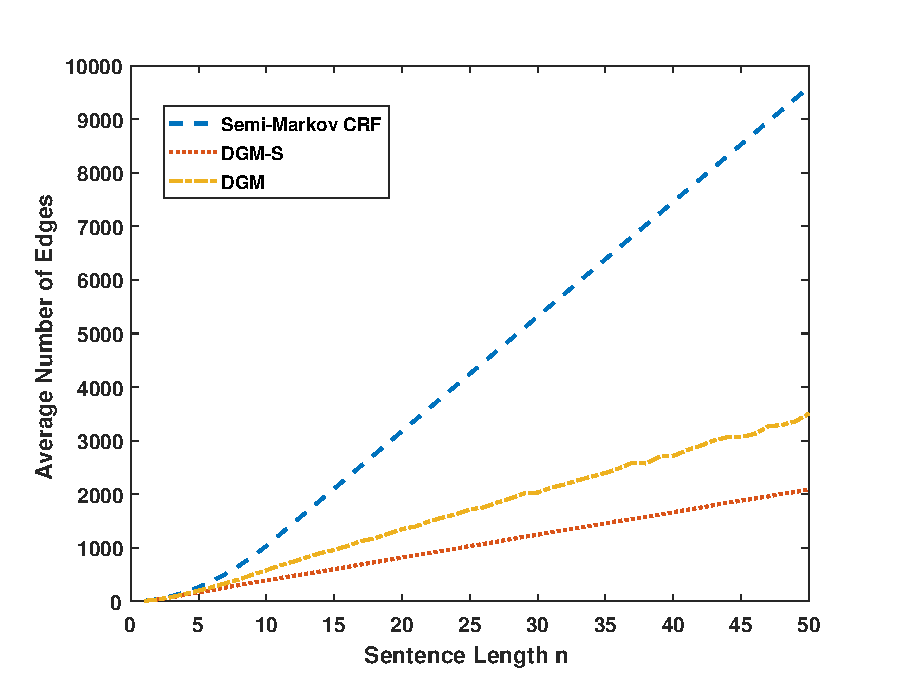
\includegraphics[width=4in]{Figures/ncomplexity.eps}
	\caption{The average number of edges over all sentences in all datasets with respect to sentence length $n$. For semi-CRF, we set $L=8$. Also note that in the dataset we have $\left\lvert T\right\rvert=5$ (\textsc{per}, \textsc{org}, \textsc{gpe}, \textsc{misc}, and special label \textsc{o} denoting non-entities)}.
	\label{fig:ncomplexity}
\end{figure}

We also calculated the average number of edges involved per token by averaging the average number of edges per token, over all sentences. More formally, let the number of sentences in a dataset be $N$,  the number of edges in $i$-th sentence be $E_i$, and the length of $i$-th sentence be $n_i$. Then the average number of edges involved per token $\bar{E}$ is:
\begin{equation*}
\bar{E} = \frac{\displaystyle\sum_{i=1}^{N}\frac{E_{i}}{n_{i}}}{N}.
\end{equation*}
Table \ref{tab:edges} shows the average number of edges involved per token for different models.
Since the number of edges in our models is linear in terms of $n$, the average number of edges per token will be constant, plus some small variance accounting for the boundary cases in the data.
%Because \textsc{dgm-s} model has an equivalent time complexity to linear-chain CRFs, the number of possible edges for each token will always be the same. 
%\textsc{dgm} also has a stable number of possible edges and though it is about 20 edges more than \textsc{dgm-s} but still much lower than semi-CRFs. 
This also explains the fact that both \textsc{dgm-s} and \textsc{dgm} models perform much faster compared to the semi-CRF model.

\begin{table}[h!]
	\centering
	\begin{tabular}{lcccccccc}
		\toprule
		& ABC & CNN  & MNB & NBC & P2.5 & PRI & VOA & Avg. \\ 
		\midrule
		\textsc{dgm-s} & 39.1 & 39.8 & 37.9 & 38.9 & 40.9 & 39.8 & 40.7 &39.5\\
		\textsc{dgm} & 57.3 & 62.9 & 53.7 & 56.2 & 71.3 & 59.8 & 65.5& 61.0  \\
		semi-CRFs & 117.8 & 133.9 & 110.3 & 119.8 & 172.4 & 126.4 & 144.3 & 132.1 \\\bottomrule
	\end{tabular}
	\caption{The average number of possible edges involved in each token when we construct the model. }
	\label{tab:edges}
\end{table}




%-----------------------------------
%	SUBSECTION 2
%-----------------------------------

\section{Experimental Setup}
For experiments, we followed~\cite{finkel2009joint} and used the Broadcast News section of the OntoNotes dataset.
Instead of using its earlier 2.0 release, we used the final release --  release 5.0 of the dataset, which is available for download\footnote{https://catalog.ldc.upenn.edu/LDC2013T19/}.
The dataset includes the following 6 subsections: ABC, CNN, MNB, NBC, PRI and VOA. 
Moreover, the current OntoNotes 5.0 release also includes some English P2.5 data, which consists of corpus translated from Chinese and Arabic.\footnote{The OntoNotes 5.0 dataset also contains the earlier release from OntoNotes 1.0 to OntoNotes 4.0. However, we found the number of sentences of the Broadcast News in the current OntoNotes 5.0 dataset does not match the number reported in \cite{finkel2009joint,finkel2010hierarchical}, which was based on OntoNotes 2.0. Furthermore, they removed some instances which are inconsistent with their model. We thus cannot conduct experiments to compare against the results reported in their work.}
Following~\cite{finkel2009joint}, we split the first 75\% of the data for training and performed evaluations on the remaining 25\%.
We set $L=8$, which can cover all entities in our dataset, and developed the $L_2$ coefficient using cross-validation (see supplementary material S.1 for details). 
%However, there is no dependency annotation in OntoNotes 5.0 dataset. 
Following previous works on dependency parsing~\cite{chen2014fast}, we preprocessed the dataset using the Stanford CoreNLP\footnote{http://stanfordnlp.github.io/CoreNLP/} to convert the constituency trees to basic Stanford dependency~\cite{de2006generating} trees. 
% The LTH Constituent-to-Dependency conversion tool cannot deal with the tag in ontonotes treebanks such as META and EDITED. 
%\footnote{Following previous work~\cite{??}, we ignored sentences with certain special tags such as META and EDITED that do not appeared in the penn treebank.}.
In our NER experiments, in addition to using the given dependency structures converted from the constituency trees, we also trained a popular transition-based parser, MaltParser\footnote{http://maltparser.org/}~\cite{nivre2006maltparser}, using the training set and then used this parser to predict the dependency trees on the test set to be used in our model. 
%
%applied the dependency prediction as the known structures. 





We also looked at the SemEval-2010 Task 1 OntoNotes English corpus\footnote{https://catalog.ldc.upenn.edu/LDC2011T01/}, which contains sentences with both dependency and named entity information.
Although this dataset is a subset of the OntoNotes dataset, it comes with manually annotated dependency structures.
%We conducted experiments on this dataset and reported the results in the supplementary material (S.2).
%The results on this dataset are consistent with the findings reported in this chapter.
%Similar conclusions as discussed in this section can be drawn based on this dataset.



%evaluation method as in the CONLL 2003 \textit{conlleval}\footnote{http://www.cnts.ua.ac.be/conll2000/chunking/output.html}.


\subsection{Features}
In order to make comparisons, we implemented a linear-chain CRFs model as well as a semi-Markov CRFs model to serve as baselines. 
The features we used are basic features which are commonly used in linear-chain CRFs and semi-CRFs. 
For the linear-chain CRFs, we consider the current word/POS tag, the previous word/POS tag, the current word shape, the previous word shape, prefix/suffix of length up to 3, as well as transition features. 
For word shape features, we followed \cite{finkel2005exploring} to create them. 
For the semi-CRFs model, we have the following features for each segment: the word/POS tag/word shape before and after the segment, indexed words/POS tags/word shapes in current segment, surface form of the segment, segment length, segment prefix/suffix of length up to 3, the start/end word/tags of current segment, and the transition features. 

Inspired by \citet{ling2012fine}, we applied the following dependency features for all models: (1) current word in current position/segment and its head word (and its dependency label); (2) current POS tag in current position/segment and its head tag (and  dependency label). More details of features can be found in the supplementary material (S.4).


\subsection{Feature Representations}
This section gives an example on the feature representation defined in Features section in the main paper. 
For illustration purpose, we take the first sentence of Figure 1 in the main paper as an example. 
The code released has the detailed feature implementation as well.

Say that we are currently at the position of word ``\textit{Ami}''. The features in the linear-chain CRF model is represented in table \ref{tab:linearf}. In semi-CRFs model, the features are defined over segment. We take the segment ``\textit{Shlomo Ben - Ami}'' as an example to describe the features in Table \ref{tab:semif}.

\begin{table}[h!]
	\centering
	\begin{tabular}{ll}
		\toprule
		Features & Examples \\ \hline
		current word & \textit{Ami} \\ 
		current POS & NNP \\ 
		previous word & \textit{-} \\ 
		previous POS & HYPH \\ 
		current word shape & Xxx \\ 
		previous word shape & - \\ 
		prefix up to length 3 & \textit{A}, \textit{Am}, \textit{Ami} \\ 
		suffix up to length 3 & \textit{i}, \textit{mi}, \textit{Ami} \\ 
		transition & \textsc{i-per} + \textsc{i-per} \\
		\midrule
		\midrule
		Dependency features & Examples \\
		\midrule 
		current word + head & \textit{Ami} + \textit{gave} \\ 
		current word + head + label & \textit{Ami} + \textit{gave} + nsubj \\ 
		current POS + head POS & NNP + VBD \\ 
		current POS + head POS + label & NNP + VBD + nsubj \\ 
		\bottomrule 
	\end{tabular}\quad 
	\caption{The features for the example sentence in the linear-chain CRFs model.}
	\label{tab:linearf}
\end{table}


\begin{table}[h!]
	\centering
	\begin{tabular}{ll}
		\toprule 
		Features & Examples \\ 
		\midrule
		word before segment & \textit{Minister} \\ 
		POS before segment & NNP \\ 
		word shape before segment & Xxxx \\ 
		word after segment & \textit{gave} \\ 
		POS after segment & VBD \\ 
		word shape after segment & xxxx \\ 
		prefix up to length 3 & \textit{S}, \textit{Sh}, \textit{Shl} \\ 
		suffix up to length 3 & \textit{i}, \textit{mi}, \textit{Ami} \\ 
		start word & start:+\textit{Shlomo} \\ 
		end word & end:+\textit{Ami} \\ 
		start POS & start POS:+NNP \\ 
		end POS & end POS:+NNP \\ 
		segment length & 4 \\ 
		transition & \textsc{o} + \textsc{per} \\ 
		indexed word & 1:\textit{Shlomo}, 2:\textit{Ben}, 3:\textit{-}, 4:\textit{Ami} \\ 
		indexed POS & 1:NNP, 2:NNP, 3:HYPH, 4:NNP \\ 
		indexed shape & 1:Xxxx, 2:Xxx, 3:-, 4:Xxx \\ 
		the whole segment & \textit{Shlomo Ben - Ami} \\ 
		dependency & same as dependency features in Table \ref{tab:linearf} \\ \bottomrule
		
	\end{tabular}\quad 
	%	\begin{tabular}{|l|l|}
	%		\hline 
	%		Features & Examples \\ \hline
	%		
	%	\end{tabular}
	\caption{The features for the example sentence in the semi-CRFs model.}
	\label{tab:semif}
\end{table}



\subsection{Data Statistics}
There are in total 18 well-defined named entity types in the OntoNotes 5.0 dataset. 
Since majority of the entities are from the following three types: \textsc{per} ({\em person}), \textsc{org} ({\em organization}) and \textsc{gpe} ({\em geo-political entities}), following \cite{finkel2009joint}, we merge all the other entity types into one general type, \textsc{misc} ({\em miscellaneous}). 
%In other words, we consider the following four distinct entity types: \textsc{per}, \textsc{org}, \textsc{gpe} and \textsc{misc}. 
Table \ref{tab:dgmstatistics} shows the statistics of total number of sentences and entities.


\begin{table}[h!]
	\centering
	
	\begin{tabular}{lrrrrr}
		\toprule
		\multirow{2}{*}{} & \multirow{2}{*}{\# Sent.} & \multicolumn{3}{c}{\# Entities}\\
		\cline{3-5}
		&&\multicolumn{1}{c}{\textsc{all}}&\multicolumn{1}{c}{\textsc{dgm-s}}&\multicolumn{1}{c}{\textsc{dgm}}\\
		\midrule
		Train                   & 9,996                        & 18,855                         & 17,584 (93.3\%)               & 18,803 (99.7\%)                 \\
		Test			& 3,339                          & 5,742                         & 5,309 (92.5\%)               & 5,720 (99.6\%)               \\
		%		\hline
		\bottomrule
	\end{tabular}
	
	\caption{Dataset statistics. }
	\label{tab:dgmstatistics}
\end{table}

% in all the subsections. 

%\begin{table}[h]
%	\centering
%	\begin{tabular}{c|rrrr}
%		& \multicolumn{2}{c}{Train+Dev} &  \multicolumn{2}{c}{Test} \\ 
%		& \# Sent.  & \# Entity & \# Sent. 	& \# Entity  \\\hline
%		ABC & 859   & 950 		& 286   	& 330 \\ 
%		CNN & 4,148 & 4,514 	& 1,382 	& 1,115 \\ 
%		MNB & 478   & 475 		& 159  		& 111  \\ 
%		NBC & 479   & 691 		& 160 		& 210 \\ 
%		PRI & 1,536 &2,449  	& 512		& 772 \\ 
%		VOA & 1,423 & 3,228   	& 474		& 1,131
%	\end{tabular}
%	\caption{Dataset Statistics. The number of sentences and entities in the OntoNotes 5.0 dataset. }
%	\label{tab:statistics}
%\end{table}

To show the relationships between the named entities and dependency structures, we present the number and percentage of entities that can be handled by our \textsc{dgm-s} model and \textsc{dgm} model respectively.
The entities that can be handled by \textsc{dgm-s} should be covered by a single arc as indicated in our model section. As for \textsc{dgm}, the entity spans should be {\em valid} as in definition 1. 
Overall, we can see that 93.3\% and 92.5\% of the entities can be handled by the \textsc{dgm-s} model in training set and test set, respectively. 
These two numbers for \textsc{dgm} are much higher -- 99.7\% and 99.6\%. 
With the predicted dependency structures in test set, 91.7\% of the entities can be handled by the \textsc{dgm-s} model, while for \textsc{dgm} it is 97.4\%.


These numbers confirm that it is indeed the case that most named entities do form {\em valid spans}, even when using predicted dependency trees,
and that such global structured information of dependency trees can be exploited for NER.

\subsection{Detailed Data Statistics and Parameter Tuning}
Table \ref{tab:detailedstatistics} shows the detailed statistics of all subsections. 
Overall, over 99.6\% entities are representable in \textsc{dgm} model and around 91\% to 94\% entities are representable \textsc{dgm-s} model. 
\begin{table}[h]
	
	\centering
	\resizebox{1\linewidth}{!}{
	\begin{tabular}{lrrrrrrrr}
		\toprule
		& \multicolumn{4}{c}{Train} & \multicolumn{4}{c}{Test} \\
		& \multirow{2}{*}{\# Sent.} & \multicolumn{3}{c}{\# Entity} & \multirow{2}{*}{\# Sent.} & \multicolumn{3}{c}{\# Entity}\\
		&&\multicolumn{1}{c}{\textsc{all}}&\multicolumn{1}{c}{\textsc{dgm-s}}&\multicolumn{1}{c}{\textsc{dgm}}  &&\multicolumn{1}{c}{\textsc{all}}&\multicolumn{1}{c}{\textsc{dgm-s}}&\multicolumn{1}{c}{\textsc{dgm}}\\
		\midrule
		ABC                   & 873                          & 1,365                         & 1,281 (93.9\%)               & 1,360 (99.6\%)                	& 292                         & 444                           & 415 (93.5\%)               & 444 (100.0\%)                \\
		CNN                   & 4,318                        & 6,627                        & 6,113 (92.2\%)              & 6,609 (99.7\%)                & 1,440                        & 1,620                         & 1,474 (91.0\%)               & 1,613 (99.6\%)                \\
		MNB                   & 477                          & 690                           & 653 (94.6\%)               & 689 (99.9\%)                	& 160                          & 177                           & 162 (91.5\%)                & 176 (99.4\%)                \\
		NBC                   & 480                         & 922                           & 868 (94.1\%)               & 918 (99.6\%)                 & 161                          & 343                           & 312 (91.0\%)               & 340 (99.1\%)                \\
		P2.5                   & 890                          & 1,995                          & 1,827 (91.6\%)               & 1,988 (99.7\%)                 	& 298                          & 672                           & 616 (91.7\%)               & 669 (99.6\%)                \\
		PRI                   & 1,536                        & 3,096                         & 2,916 (94.2\%)               & 3,090 (99.8\%)                 	& 513                          & 992                           & 927 (93.5\%)               & 990 (99.8\%)                \\
		VOA                   & 1,422                        & 4,160                         & 3,926 (94.4\%)               & 4,149 (99.7\%)                 	& 475                          & 1,494                         & 1,403 (93.9\%)               & 1,488 (99.6\%)               \\	
		Total                   & 9,996                        & 18,855                         & 17,584 (93.3\%)               & 18,803 (99.7\%)                 & 3,339                          & 5,742                         & 5,309 (92.5\%)               & 5,720 (99.6\%)               \\
		\bottomrule
		%		\hline
		%		\multirow{2}{*}{Test} & \multirow{2}{*}{\# Sent.} & \multicolumn{3}{c}{\# Entity}\\
		%		\cline{3-5}
		%		&&\multicolumn{1}{c}{\textsc{all}}&\multicolumn{1}{c}{\textsc{dgm-s}}&\multicolumn{1}{c}{\textsc{dgm}}\\
		%		\hline
		%		ABC			& 292                         & 444                           & 415 (93.5\%)               & 444 (100.0\%)                \\
		%		CNN			& 1,440                        & 1,620                         & 1,474 (91.0\%)               & 1,613 (99.6\%)                \\
		%		MNB			& 160                          & 177                           & 162 (91.5\%)                & 176 (99.4\%)                \\
		%		NBC			& 161                          & 343                           & 312 (91.0\%)               & 340 (99.1\%)                \\
		%		P2.5			& 298                          & 672                           & 616 (91.7\%)               & 669 (99.6\%)                \\
		%		PRI			& 513                          & 992                           & 927 (93.5\%)               & 990 (99.8\%)                \\
		%		VOA			& 475                          & 1,494                         & 1,403 (93.9\%)               & 1,488 (99.6\%)               \\
		%		Total			& 3,339                          & 5,742                         & 5,309 (92.5\%)               & 5,720 (99.6\%)               \\
	\end{tabular}
}
	\caption{Dataset Statistics. The number of sentences and entities in the Broadcast News corpus of OntoNotes 5.0 dataset. }
	\label{tab:detailedstatistics}
\end{table}
We tuned the $L_{2}$ regularization parameter using 10-fold cross-validation for all the models. 
Specifically for each model, we performed cross validation on the largest subsection, CNN, and obtained the best parameter with highest average F-score. 
We then used this parameter for other subsections as well. 
The values of $L_{2}$ regularization parameter we evaluated is $[0.0001, 0.001, 0.01, 0.1, 1]$. Specifically, we have four models and each of them is associated with two variants with or without dependency features. 
We obtained the best regularization parameter 0.1 for all the models except the \textsc{dgm-s} without dependency features, whose best regularization parameter is 1. 


%\subsection{Hyper-parameter}
%
%The only hyper-parameter involved in all models is the $L_{2}$ regularization coefficient.
%We tuned it for each model using cross-validation on the training set.
%Specifically, we performed 10-fold cross-validation of the coefficient from the set $[0.0001, 0.001, 0.01, 0.1, 1]$ on the training set of the largest section -- CNN.
%The resulting  coefficients are then used for all experiments for respective models.

\section{Results and Discussions}
%\begin{table*}[h]
%	\centering
%	\begin{tabular}{c|ccc|ccc|ccc|ccc}
%		\multirow{3}{*}{F-score}& \multicolumn{6}{c|}{using given dependency structure} &\multicolumn{6}{c}{using predicted dependency structure} \\
%		& \multicolumn{3}{c|}{w/o Dep features} &\multicolumn{3}{c|}{w Dep features}
%		& \multicolumn{3}{c|}{w/o Dep features} &\multicolumn{3}{c}{w Dep features} \\
%		& Semi   & SDG   & MDG   
%		& Semi   & SDG   & MDG
%		& Semi   & SDG   & MDG   
%		& Semi   & SDG   & MDG \\ \hline
%		ABC&	73.44 &	71.19 &	\textbf{74.62} 
%		& 73.91 & 71.77 & \textbf{74.47}
%		& 73.44 & 71.19 & \textbf{74.20} 
%		& 74.02 & 71.36 & \textbf{74.47}\\
%		CNN&		73.14&	72.50 &	\textbf{74.16} 
%		&  73.35 & 73.33 & \textbf{73.60} 
%		& 73.14 & 72.26 & \textbf{73.46} 
%		& 72.64 & 72.33 & \textbf{72.64} \\ 
%		MNB&	74.44 &	72.40 &		\textbf{75.34}
%		&  76.99 & 73.21 & \textbf{77.33}
%		& 74.44 & 72.73 & \textbf{75.43}
%		& \textbf{76.99} & 73.21 & 76.65 \\
%		NBC&	72.47 &	68.72&	\textbf{73.07}
%		&  \textbf{70.40} & 68.08 & 70.23 
%		& 72.47 & 68.41 & \textbf{72.60}
%		& \textbf{71.30} & 68.40 & 71.00\\
%		PRI	&		84.79&	85.81&	\textbf{87.52}
%		&  86.10 & 85.90 & \textbf{87.10} 
%		& 84.79 & 85.36 & \textbf{86.61}
%		& \textbf{86.51} & 84.82 & 86.20\\
%		VOA	&		83.62&	84.85&	\textbf{85.57}
%		& 85.08 & 85.17 & \textbf{85.45}
%		& 83.62 & 84.31 & \textbf{85.04}
%		& \textbf{85.13} & 85.00 & \textbf{85.13}\\
%		Overall &  78.84 &  &
%		&  & &  
%		& 78.84 & &
%		& 79.57 & &
%	\end{tabular}
%	\caption{Named Entity Recognition (with both given and predicted dependency structures) Results on OntoNotes 5.0 dataset}
%	\label{tab:nerresult}
%\end{table*}






\subsection{NER Performance}
Following previous work~\cite{finkel2009joint}, we report standard  F-score in this section (detailed results with precision and recall can be found in the supplementary material S.5). 
Table \ref{tab:ner_withdpfeatures} shows the results of all models when  dependency features are exploited.
Specifically, it shows results when the given and predicted dependency trees are considered, respectively.
Overall, the semi-Markov CRFs, \textsc{dgm-s} and \textsc{dgm} models perform better than the linear-chain CRFs model. 
Our \textsc{dgm} model obtains an overall F-score at 80.5\%  and outperforms the semi-CRFs model significantly ($p<0.001$ with bootstrap resampling~\cite{koehn2004statistical}).
%and achieve a significant level with $p<0.001$ against semi-CRF. 
For individual subsection, our \textsc{dgm} also performs the best.
On 2 out of the 7 subsections, our model's improvements over the baseline semi-CRFs model are significant ($p<0.001$ with bootstrap resampling).
For some other subsections like ABC, CNN, MNB, NBC and PRI, \textsc{dgm} has higher F-score than the semi-CRFs model but the improvements are not statistically significant.
The results show that comparing with  semi-CRFs, our \textsc{dgm} model, which has a lower average-case time complexity, still maintains a competitive performance. 
Such results confirm that the global structured information conveyed by dependency trees are useful and can be exploited by our \textsc{dgm} model.

\begin{table*}[h!]
	\centering
	\resizebox{1.0\linewidth}{!}{
		\begin{tabular}{crcccccccc}
			\toprule
			Dependency	& Model                  & ABC                               & CNN                               & MNB                               & NBC                               & P2.5                              & PRI                               & VOA  &Overall                           \\ 
			\midrule
			\multirow{4}{*}{Given}&Linear-chain CRFs & 70.2                              & 75.9                              & \textbf{75.7}                     & 65.9                              & 70.8                              & 83.2                              & 84.6                              & 77.8                              \\
			&Semi-Markov CRFs  & \textbf{71.9}                     & \textbf{78.2}                     & \textbf{74.7}                     & \textbf{69.4}                     & 73.5                              & \textbf{85.1}                     & 85.4                              & 79.6                              \\
			&\textsc{dgm-s}            & 71.4                              & 77.0                              & 73.4                              & 68.4                              & 72.8                              & \textbf{85.1}                     & 85.2                              & 79.0                              \\
			& \textsc{dgm}              & \textbf{72.3}                     & \textbf{78.6}                     & \textbf{76.3}                     & \textbf{69.7}                     & \textbf{75.5}                     & \textbf{85.5}                     & \textbf{86.8}                     & \textbf{80.5}                     \\
			\midrule
			\midrule
			\multirow{4}{*}{Predicted}& Linear-chain CRFs & 68.4          & 75.4          & 74.4          & 66.3          & 70.8          & 83.3          & 83.7          & 77.3          \\
			& Semi-Markov CRFs  & \textbf{71.6} & \textbf{78.0} & 73.5          & \textbf{71.5} & \textbf{73.7}          & \textbf{84.6} & \textbf{85.3} & \textbf{79.5} \\
			&\textsc{dgm-s}            & 70.6          & 76.4          & 73.4          & 68.7          & 71.3          & \textbf{83.9} & 84.4          & 78.2          \\
			&\textsc{dgm}              & \textbf{71.9} & \textbf{77.6} & \textbf{75.4} & \textbf{71.4} & \textbf{73.9} & \textbf{84.2} & \textbf{85.1} & \textbf{79.4} \\
			\bottomrule
		\end{tabular}
	}
	\caption{NER results for all models, when given and predicted dependency trees are used and dependency features are used. Best values and the values which are not significantly different in 95\% confidence interval are put in bold.}
	\label{tab:ner_withdpfeatures}
\end{table*}



The performance of \textsc{dgm-s} is worse than that of semi-CRFs and \textsc{dgm} in general since there are still 
many named entities that can not be handled by such a simplified model (see Table \ref{tab:detailedstatistics}).
This model has the same time complexity as the linear-chain CRFs, but performs better than linear-chain CRFs, largely due to the fact that certain structured information of dependency trees are exploited in \textsc{dgm-s}.
%still a large portion of data does not satisfy \textsc{dgm-s} model, while it has a complexity with linear-chain CRFs and better performance than linear chain CRFs. 
We note that such a simplified model obtains similar results as semi-CRFs for the two larger subsections, PRI and VOA.
This is largely due to the fact that a larger percentage of the entities in these two subsections can be handled by \textsc{dgm-s}.
%These larger datasets have about 93\% of test data satisfy the model and \textsc{dgm-s} achieves similar result to semi-CRFs while having a linear-chain CRF time complexity. 
%%For some datasets, like, our model DGM performs equally better compared to semi-crf with a p value. ***
%% even though about 7\% not satisfy, our DGM-S model has a quite promising performance for those datasets.
It is noted that the performance of both semi-CRFs and \textsc{dgm} degrades when the predicted dependency trees are used instead of the given.
The drop in F-score for \textsc{dgm} is more significant as compared to the semi-CRFs.
Nevertheless, their results remain comparable.
Such experiments show the importance of considering high quality dependency structures for performing guided NER in our model.

To understand the usefulness of the global structured information of dependency trees better, we conducted further experiments by excluding dependency features from our models.
Such results are shown in Table \ref{tab:ner_withoutdpfeatures}.
Our \textsc{dgm} model consistently performs competitively with the semi-CRFs model. 
The only exception occurs when the ABC subsection is considered and the predicted dependency trees are used ($p$=0.067).
In general, we can see that when dependency features are excluded, the overall F-score for all models drop substantially.
However, we note that for semi-CRFs, the drop in F-score is 1.1\% for given dependency trees, and is 1.0\% for predicted trees,
whereas for \textsc{dgm}, the drops with given and predicted trees are both 0.6\%.
%Such results show that our model is able to effectively capture the useful global structured information of dependency trees.
Overall, such results largely show that our proposed  model is able to effectively make use of the global structured information conveyed by dependency trees for NER. 

\begin{table*}[h!]
	\centering
	\resizebox{1.0\linewidth}{!}{
		\begin{tabular}{crcccccccc}
			\toprule
			Dependency	&	Model                  & ABC           & CNN           & MNB           & NBC           & P2.5          & PRI           & VOA           & Overall       \\ 
			\midrule
			\multirow{4}{*}{Given}&Linear-chain CRFs       & \multicolumn{1}{c}{66.5}          & \multicolumn{1}{c}{74.1}          & \multicolumn{1}{c}{74.9}          & \multicolumn{1}{c}{65.4}          & \multicolumn{1}{c}{70.8}          & \multicolumn{1}{c}{82.9}          & \multicolumn{1}{c}{82.3}          & \multicolumn{1}{c}{76.3}          \\
			&Semi-Markov CRFs        & \multicolumn{1}{c}{\textbf{72.3}} & \multicolumn{1}{c}{76.6}          & \multicolumn{1}{c}{\textbf{75.0}} & \multicolumn{1}{c}{\textbf{69.3}} & \multicolumn{1}{c}{73.7}          & \multicolumn{1}{c}{84.1}          & \multicolumn{1}{c}{83.3}          & \multicolumn{1}{c}{78.5}          \\
			&\textsc{dgm-s}                  & \multicolumn{1}{c}{69.4}          & \multicolumn{1}{c}{76.1}          & \multicolumn{1}{c}{73.4}          & \multicolumn{1}{c}{68.0}          & \multicolumn{1}{c}{72.5}          & \multicolumn{1}{c}{85.2}          & \multicolumn{1}{c}{85.1}          & \multicolumn{1}{c}{78.6}          \\
			&\textsc{dgm}                    & \textbf{72.7} & \multicolumn{1}{c}{\textbf{77.2}} & \multicolumn{1}{c}{\textbf{75.8}} & \multicolumn{1}{c}{\textbf{68.5}} & \multicolumn{1}{c}{\textbf{76.8}} & \multicolumn{1}{c}{\textbf{86.2}} & \multicolumn{1}{c}{\textbf{85.5}} & \multicolumn{1}{c}{\textbf{79.9}} \\ 
			\midrule
			\midrule
			
			\multirow{4}{*}{Predicted}&Linear-chain CRFs       & 66.5          & 74.1          & 74.9          & 65.4          & 70.8          & 82.9          & 82.3           & 76.3          \\
			&Semi-Markov CRFs        & \textbf{72.3} & \textbf{76.6} & \textbf{75.0} & \textbf{69.3} & \textbf{73.7} & 84.1          & 83.3          & \textbf{78.5} \\
			&\textsc{dgm-s}                  & 69.1          & 75.6          & 73.8          & 67.2          & 72.0          & 84.5          & \textbf{84.2} & 78.0          \\
			&\textsc{dgm}                    & 71.3          & \textbf{76.2} & \textbf{75.9} & \textbf{68.8} & \textbf{74.6} & \textbf{85.1} & \textbf{84.3} & \textbf{78.8}\\
			\bottomrule
		\end{tabular}
	}
	\caption{NER results for all models, when  given and predicted dependency trees are used but dependency features are not used. Best values and the values which are not significantly different in 95\% confidence interval are put in bold.}
	\label{tab:ner_withoutdpfeatures}
\end{table*}



We have also conducted experiments on the widely-used NER dataset, CoNLL-2003, using the Stanford dependency parser\footnote{http://nlp.stanford.edu/software/nndep.shtml} to generate the dependency trees. 
Using the same feature set that we describe in this work, our models do not achieve the state-of-the-art results on this dataset. However, they still perform comparably with the semi-CRFs model, while requiring much lesser running time.
Note that since our goal in this work is to investigate the usefulness of incorporating the dependency structure information for NER, we did not attempt to tune the feature set to get the best result on a specific dataset.
Also it is worth remarking that we still obtain a relatively good performance for our \textsc{dgm} model although the dependency parser is not trained within the dataset itself and that a correct dependency structure information is crucial for the \textsc{dgm} model.

%The performance comparison becomes slightly different when we use the predicted dependency structures by MaltParser. 
%Either semi-CRFs or \textsc{dgm} does not always has a higher F-score than each other. 
%We believe the drop of \textsc{dgm} itself is caused by some wrongly classified dependencies may affect the model itself directly rather than features only. 
%However, our DGM still has a similar result compare to Semi-Markov CRF since overall the semi-CRFs is not significantly better than \textsc{dgm} in F-score ($p=0.25$). 
%Also in the experiments on MNB dataset, \textsc{dgm} performs better than semi-CRFs with $p<0.05$. 
%Again, DGM-S has a similar result on PRI dataset compared to semi-CRF ($p=0.14$) since it also has a large portion (93.5\%) of test data with predicted dependency structures satisfy \textsc{dgm-s} model. Semi-CRF is not significantly better than DGM-S on VOA dataset either ($p=0.07$) and it also has 93\% of test data with predicted dependency structures satisfy DGM-S model. 
%In our experiments, we also found that our DGM model can produce almost equivalent result even without adding the dependency information. 
%We provide the results without dependency features in our supplementary materials (S.2). 
%%We combine the results of all seven datasets for each model and apply the paired t-test for each of the two models. We obtain the significance level for F-score at $p<${\color{red}{(TODO)}} . 

%Overall, DGM can produce similar or even better performance than semi-CRF when we have well-defined dependency structures. Furthermore, both DGM-S and DGM has a much lower running time in practice, which we can see in the speed analysis in the following section. 
\begin{figure}[t!]
	%	\centering
	\begin{subfigure}[t]{0.48\columnwidth}
		\centering
		\begin{tikzpicture}[node distance=6mm and 9mm, >=Stealth, 	place/.style={draw=none, inner sep=0pt}]
		\node[place,line width=1pt, minimum size=0.2cm] (13) {\small USS};
		\node[place,line width=1pt, right=of p1, minimum size=0.2cm, xshift=-2mm] (14) {\small Cole};
		\node[place,line width=1pt, right=of p2, minimum size=0.2cm, xshift=-2mm] (15) {\small Navy};
		\node[place,line width=1pt, right=of p3, minimum size=0.2cm, xshift=0mm] (16) {\small destroyer};
		\node [place](at) [below=of 13,yshift=2.65mm]{\scriptsize NNP};
		\node [place](bt) [below=of 14,yshift=2.65mm] {\scriptsize NNP};
		\node [place](ct) [below=of 15,yshift=3.0mm] {\scriptsize NNP};
		\node [place](dt) [below=of 16,yshift=3.0mm]{\scriptsize NNP};
		\node [place](ae) [below=of at,yshift=2.45mm]{\scriptsize \textsc{b-misc}};
		\node [place](be) [below=of bt,yshift=2.5mm] {\scriptsize \textsc{i-misc}};
		\node [place](ce) [below=of ct,yshift=2.5mm] {\scriptsize \textsc{b-org}};
		\node [place](de) [below=of dt,yshift=2.5mm]{\scriptsize \textsc{o}};
		\draw [line width=1pt, -{Stealth[length=3.5mm, open]},->] (14) to [out=120,in=60, looseness=1.1] node [above] {} (13);
		\draw [line width=1pt, -{Stealth[length=3.5mm, open]},->] (16) to [out=120,in=60, looseness=0.9] node [above] {} (14);
		\draw [line width=1pt, -{Stealth[length=3.5mm, open]},->] (16) to [out=120,in=60, looseness=1.1] node [above] {} (15);
		\end{tikzpicture}
		\caption{Given dependency tree}
		\label{fig:error_given} 
	\end{subfigure}
	\begin{subfigure}[t]{0.48\columnwidth}
		\centering
		\begin{tikzpicture}[node distance=6mm and 9mm, >=Stealth, 	place/.style={draw=none, inner sep=0pt}]
		\node[place,line width=1pt, minimum size=0.2cm, xshift=7mm] (13) {\small USS};
		\node[place,line width=1pt, right=of p1, minimum size=0.2cm, xshift=5mm] (14) {\small Cole};
		\node[place,line width=1pt, right=of p2, minimum size=0.2cm, xshift=5mm] (15) {\small Navy};
		\node[place,line width=1pt, right=of p3, minimum size=0.2cm, xshift=6mm] (16) {\small destroyer};
		\node [place](at) [below=of 13,yshift=2.65mm]{\scriptsize NNP};
		\node [place](bt) [below=of 14,yshift=2.65mm] {\scriptsize NNP};
		\node [place](ct) [below=of 15,yshift=3.0mm] {\scriptsize NNP};
		\node [place](dt) [below=of 16,yshift=3.0mm]{\scriptsize NNP};
		\node [place](ae) [below=of at,yshift=2.45mm]{\scriptsize \textsc{b-org}};
		\node [place](be) [below=of bt,yshift=2.5mm] {\scriptsize \textsc{i-org}};
		\node [place](ce) [below=of ct,yshift=2.5mm] {\scriptsize \textsc{i-org}};
		\node [place](de) [below=of dt,yshift=2.5mm]{\scriptsize \textsc{o}};
		\draw [line width=1pt, -{Stealth[length=3.5mm, open]},->] (15) to [out=120,in=60, looseness=0.9] node [above] {} (13);
		\draw [line width=1pt, -{Stealth[length=3.5mm, open]},->] (15) to [out=120,in=60, looseness=1.1] node [above] {} (14);
		\draw [line width=1pt, -{Stealth[length=3.5mm, open]},->] (16) to [out=120,in=60, looseness=1.1] node [above] {} (15);
		\end{tikzpicture}
		\caption{Predicted dependency tree}
		\label{fig:error_predicted} 
	\end{subfigure}
	\caption{The effect of different dependency parses on the output of \textsc{dgm}. These are taken out from a part of a sentence. The NER result in (a) is correct, while (b) is not.}
	\label{fig:error_analysis}
\end{figure}
\subsection{Error Analysis}
We provide a further analysis of how the dependency parsing performance affects NER based on Table \ref{tab:ner_withoutdpfeatures}. 
%Because there is no dependency features involved in the model but the dependency structure information instead. 
Because our model uses the dependency structure information directly instead of using them as features, we can analyze the influence of dependency structures on NER more clearly.
Specifically, we focus on how the dependency parsing results affect the prediction of our \textsc{dgm} model. 

A typical error made by our model taken from the results is shown in Figure \ref{fig:error_analysis} where the dependency tree in Figure \ref{fig:error_given} is given by the conversion of constituent parse tree and the other one in Figure \ref{fig:error_predicted} is predicted from the MaltParser. 
The NER result on the left is correct while the one on the right is incorrect. 
%We found that this is a typical error made by our model.
Based on the predicted dependency structure in Figure \ref{fig:error_predicted}, there is no way to predict an entity type for ``{\em USS Cole}'' since this is not a valid span in \textsc{dgm} model. 
Furthermore, \textsc{dgm} can actually recognize ``{\em Navy}'' as an \textsc{org} entity even though the predicted dependency is incorrect. 
But the model considers ``{\em USS Cole Navy}'' as an entity due to the interference of other entity features ({\em e.g.}, NNP tag and Capitalized pattern) that ``{\em USS Cole}'' has. 
While with the given dependency tree, \textsc{dgm} considers ``{\em USS Cole}'' as a valid span and correctly recognizes it as a \textsc{misc} entity. 


\subsection{Speed Analysis}
From Figure \ref{fig:graphexample} we can see that the running time required for each model depends on the number of edges that the model considers.
We thus empirically calculated the average number of edges per word each model considers based on our training data.
We found that the average number of edges involved in each token is 132 for the semi-CRFs model,
while this number becomes 40 and 61 for \textsc{dgm-s} and \textsc{dgm} respectively.
A lower number of edges indicates less possible structures to consider, and a reduced running time.
See more detailed information  in the supplementary material (S.3.2).

%More number of possible edges in Figure \ref{fig:graphexample} makes the inference slower since all of them are considered during the inference process.  
%We calculated the number of possible edges for each sentence, summed up this number over all sentences and then averaged it by the number of sentences. 
%The average number of edges involved in each token is 132 for semi-CRF while this statistics are 40 and 61 for DGM-S and DGM, respectively. 
%Lower number of edges gives us less possible structures, which help us reduce the searching space. 
%%can show the table if I still have some spaces. 
The results on training time per iteration (inference time) for all 7 subsections are shown in Figure \ref{fig:time}. 
From the figure we can see that the linear-chain CRFs model empirically runs the fastest.
The simple \textsc{dgm-s} model performs comparably with linear-chain CRFs.
The semi-CRFs model requires substantially longer time due to the additional factor $L$ (set to 8 in our experiments) in its time complexity.
In contrast, our model \textsc{dgm} requires only 47\% of the time needed for semi-CRFs for each training iteration, and requires 37\% more time than the \textsc{dgm-s} model.
%Such results match our theoretical analysis well.

%The linear-chain CRFs model serves as a baseline which has the fastest speed because it has the lowest time complexity among four models. 
%It is obvious to see that the conventional semi-CRFs is the slowest one on every dataset. 
%Since our \textsc{dgm-s} has the theoretically same complexity as the linear-chain CRFs, the inference time is slightly slower than Linear-chain CRF but much faster than the conventional semi-CRF. 
%For our DGM, though it has a higher complexity than DGM-S on average, the inference time is still much faster than the conventional semi-CRF over each of the seven datasets. 
%Empirically, the running time of \textsc{dgm} is 1.37 times more than \textsc{dgm-s} but 47\% of semi-CRF, especially for the larger dataset like CNN, PRI and VOA. Even though when the dataset size is small, the speed improvement by \textsc{dgm} is significant, with about 46\% running time of semi-CRF on ABC, MNB and NBC datasets.  

\begin{figure}[h!]
	\centering
	\scalebox{1}{
		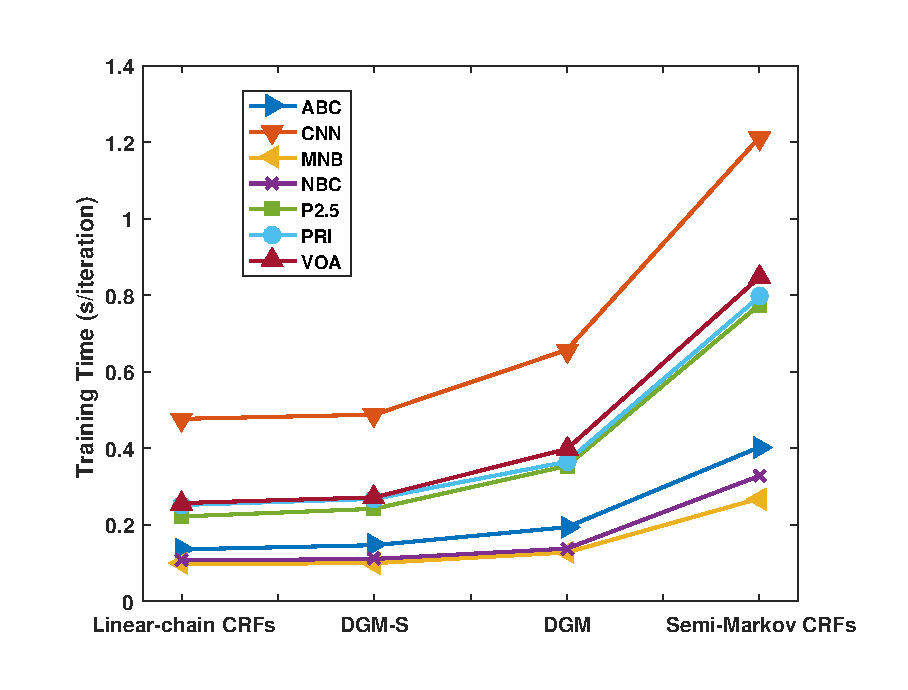
\includegraphics[width=4in]{Figures/decode_bold.eps}
	}
	\caption{Training time per iteration of all the models.}
	\label{fig:time}
\end{figure}

%\begin{table}[h]
%	\centering
%	\begin{tabular}{c|c|c}
%		Decoding Time & without  & with  \\
%		(s/sent) 		& dep features & dep features \\ \hline
%		Semi-Markov	& 1.008&	1.362 \\
%		%Linear-chain &	0.318&	0.344\\
%		DGM-S				& 0.354&	0.430 \\
%		DGM			& 0.704&	0.803 \\
%	\end{tabular}
%	\caption{The decoding time of all the models on OntoNotes 5.0 dataset}
%	\label{tab:decodingtime}
%\end{table}
%%Use matlab to draw a graph tomorrow, basically two lines.



\subsection{Results on SemEval-2010 Task 1 Dataset}

The dataset in SemEval-2010 Task 1 is a subset of OntoNotes English corpus. The dependency and named entities information are annotated in this dataset. 
There are a total of 3,648 sentences with 4,953 entities in the training set, 741 sentences with 1,165 entities in the development set, and 1,141 sentence with 1,697 entities in the test set. 
In this dataset, we found that overall 92.7\% of entities are representable in \textsc{dgm-s} and 96.6\% of entities are representable in \textsc{dgm}. 
%%Talks about the number of entities as well.

Table \ref{tab:semres} and Table \ref{tab:semnodepres} show the NER performance of all models on SemEval 2010 Task 1 dataset. In Table \ref{tab:semres}, the semi-CRF model with gold dependency features has a higher F-score while it is not significantly better than our \textsc{dgm} ($p=0.44$). 
However, \textsc{dgm} performs worse when the predicted dependency is used as features since the percentages of entities representable in \textsc{dgm} is not as high as 99\% in the other dataset, and also the predicted dependency information affects our \textsc{dgm} model structures. Furthermore, if we do not use the dependency features, both \textsc{dgm} and semi-CRFs perform similarly, with p-values of $p=0.23$ and $p=0.33$ when using gold and predicted dependency structures for \textsc{dgm}, respectively. The Semi-CRF model achieves 74.5\% F-score while \textsc{dgm} (using gold dependency structures) achieves 74.8\% F-score with a much faster training time per iteration (inference time). The inference time of semi-CRFs on this dataset is 2.25 times more than the inference time of \textsc{dgm}. 
%%mentioned about the percentage here as well.
\begin{table*}[t!]
	\centering
	\resizebox{\columnwidth}{!}{
		\begin{tabular}{lcllllllllllll}
			\toprule
			& \multirow{2}{*}{Dependency}& \multicolumn{3}{c}{Linear-chain CRFs}                                   & \multicolumn{3}{c}{Semi-Markov CRFs}                                   & \multicolumn{3}{c}{\textsc{dgm-s}}                                              & \multicolumn{3}{c}{\textsc{dgm}}                                              \\
			& & \multicolumn{1}{c}{\em P} & \multicolumn{1}{c}{\em R} & \multicolumn{1}{c}{\em F} & \multicolumn{1}{c}{\em P} & \multicolumn{1}{c}{\em R} & \multicolumn{1}{c}{\em F} & \multicolumn{1}{c}{\em P} & \multicolumn{1}{c}{\em R} & \multicolumn{1}{c}{\em F} & \multicolumn{1}{c}{\em P} & \multicolumn{1}{c}{\em R} & \multicolumn{1}{c}{\em F} \\ \midrule
			\multirow{2}{*}{SemEval 2010}&Gold & 	75.8&	72.2&	73.9&77.3&73.8&\textbf{75.5}	&	76.1&	72.4&	74.2&	77.0&	73.0&	\textbf{75.0} \\
			&Predicted & 	75.2&	71.1&	73.1&77.2&73.2&\textbf{75.1}	&	76.0&	72.2&	74.1&	76.4&	71.8&	74.1  \\
			\bottomrule        
			% check the t-test score tomorrow 75.1>74.1 p<0.01
		\end{tabular}
	}
	\caption{Named Entity Recognition Results on the SemEval 2010 Task 1 dataset. All the models in this table use the dependency information as features.}
	\label{tab:semres}
\end{table*}

\begin{table*}[t!]
	\centering
	\resizebox{\columnwidth}{!}{
		\begin{tabular}{lcllllllllllll}
			\toprule
			& \multirow{2}{*}{Dependency}& \multicolumn{3}{c}{Linear-chain CRFs}                                   & \multicolumn{3}{c}{Semi-Markov CRFs}                                   & \multicolumn{3}{c}{\textsc{dgm-s}}                                              & \multicolumn{3}{c}{\textsc{dgm}}                                              \\
			& & \multicolumn{1}{c}{\em P} & \multicolumn{1}{c}{\em R} & \multicolumn{1}{c}{\em F} & \multicolumn{1}{c}{\em P} & \multicolumn{1}{c}{\em R} & \multicolumn{1}{c}{\em F} & \multicolumn{1}{c}{\em P} & \multicolumn{1}{c}{\em R} & \multicolumn{1}{c}{\em F} & \multicolumn{1}{c}{\em P} & \multicolumn{1}{c}{\em R} & \multicolumn{1}{c}{\em F} \\ \midrule
			\multirow{2}{*}{SemEval 2010}&Gold & 	\multirow{2}{*}{76.1}&	\multirow{2}{*}{71.2}&		\multirow{2}{*}{73.6}&\multirow{2}{*}{77.2}&\multirow{2}{*}{72.1}&\multirow{2}{*}{\textbf{74.5}	}&	77.1&	71.6&	74.3& 77.7  &	72.1& \textbf{74.8} \\ %%p=0.23
			&Predicted & 	&	&	&&&	&	77.0&	71.2&	74.0&	77.3&	71.5&	\textbf{74.3}     %% 0.33  
			\\\bottomrule 	  
			% check the t-test score tomorrow 
		\end{tabular}
	}
	\caption{Named Entity Recognition Results on the SemEval 2010 Task 1 dataset without dependency features. Note that \textsc{dgm-s} and \textsc{dgm} still utilize the dependency information to build the models.}
	\label{tab:semnodepres}
\end{table*}




\subsection{Full Results with Precision, Recall and F-score}
This section presents the full results with precision, recall and F-score of all models in the paper. 
Table \ref{tab:nerresult} and Table \ref{tab:prednerresult} show the results with dependency features while Table \ref{tab:nerresultnodep} and Table \ref{tab:prednerresultnodep} show the results without dependency features. 
Recall that our \textsc{dgm-s} and \textsc{dgm} models use the dependency structure information to build the models even if we don't use the dependency features. 

%Table \ref{tab:nerresult} shows the performance of using gold dependency structured information in \textsc{dgm-s} and \textsc{dgm}. Overall, \textsc{dgm} significantly outperforms semi-CRFs in F-score with $p<0.0001$. 
%\textsc{dgm} has a lower F-score in NBC dataset but with $p=0.26$, which indicates semi-CRFs is not significantly better than \textsc{dgm}. 
%The performance of \textsc{dgm-s} and \textsc{dgm} using the predicted dependency structured information is shown in Table \ref{tab:prednerresult}. Compared to overall \textsc{dgm} result in Table \ref{tab:nerresult}, the performance of \textsc{dgm} using predicted dependency structure drops 1.1\% and it's not significantly better than CRFs though having a higher F-score. 
\begin{table*}[h!]
	\centering
	\scalebox{0.8}{
		\begin{tabular}{lllllllllllll}
			\toprule
			
			& \multicolumn{3}{c}{Linear-chain CRFs}                                   & \multicolumn{3}{c}{Semi-Markov CRFs}                                   & \multicolumn{3}{c}{\textsc{dgm-s}}                                              & \multicolumn{3}{c}{\textsc{dgm}}                                              \\
			& \multicolumn{1}{c}{\em P} & \multicolumn{1}{c}{\em R} & \multicolumn{1}{c}{\em F} & \multicolumn{1}{c}{\em P} & \multicolumn{1}{c}{\em R} & \multicolumn{1}{c}{\em F} & \multicolumn{1}{c}{\em P} & \multicolumn{1}{c}{\em R} & \multicolumn{1}{c}{\em F} & \multicolumn{1}{c}{\em P} & \multicolumn{1}{c}{\em R} & \multicolumn{1}{c}{\em F} \\ \midrule
			ABC& 	71.5&	68.9&	70.2&	71.7&	72.2&	\textbf{71.9}&	71.3&	71.5&	71.4&	72.2&	72.4&	\textbf{72.3}\\
			CNN&	76.7&	75.1&	75.9&	78.3&	78.2&	\textbf{78.2}&	77.2&	76.9&	77.0&	78.7&	78.6&	\textbf{78.6}\\
			MNB&	80.8&	71.2&	75.7&	77.4&	72.2&	\textbf{74.7}&	76.5&	70.5&	73.4&	78.8&	73.9&	\textbf{76.3}\\
			NBC&	69.0&	63.0&	65.9&	70.7&	68.2&\textbf{69.4}&	70.3&	66.7&	68.4&	70.3&	69.1&	\textbf{69.7}\\
			P2.5&	73.2&	68.6&	70.8&	75.0&	72.0&	73.5&	74.7&	70.9&	72.8&	76.7&	74.4&	\textbf{75.5}\\
			PRI&	83.9&	82.6&	83.2&	84.7&	85.5&	\textbf{85.1}&	84.8&	85.4&	\textbf{85.1}&	85.1&	85.9&	\textbf{85.5}\\
			VOA&	85.7&	83.5&	84.6&	85.6&	85.2&	85.4&	85.2&	85.1&	85.2&	87.1&	86.4&	\textbf{86.8}\\
			Overall&79.2&	76.5&	77.8&	79.9&	79.3&	79.6&	79.5&	78.6&	79.0&	80.8&	80.2&	\textbf{80.5}            \\
			\bottomrule   
		\end{tabular}
	}
	
	\caption{Named Entity Recognition Results on the Broadcast News corpus of OntoNotes 5.0 dataset. All the models in this table are using the gold dependency information. Both \textsc{dgm-s} and \textsc{dgm} models apply the dependency information in two ways: building the model and as well as using them as features.}
	\label{tab:nerresult}
\end{table*}

\begin{table*}[h!]
	\centering
	\scalebox{0.8}{
		
		\begin{tabular}{lllllllllllll}
			\toprule
			& \multicolumn{3}{c}{Linear-chain CRFs}                                   & \multicolumn{3}{c}{Semi-Markov CRFs}                                   & \multicolumn{3}{c}{\textsc{dgm-s}}                                              & \multicolumn{3}{c}{\textsc{dgm}}                                              \\
			& \multicolumn{1}{c}{\em P} & \multicolumn{1}{c}{\em R} & \multicolumn{1}{c}{\em F} & \multicolumn{1}{c}{\em P} & \multicolumn{1}{c}{\em R} & \multicolumn{1}{c}{\em F} & \multicolumn{1}{c}{\em P} & \multicolumn{1}{c}{\em R} & \multicolumn{1}{c}{\em F} & \multicolumn{1}{c}{\em P} & \multicolumn{1}{c}{\em R} & \multicolumn{1}{c}{\em F} \\ \midrule
			ABC&	70.1&	66.7&	68.4&	71.4&	71.7&	\textbf{71.6}&	70.6&	70.6&	70.6&	71.8&	72.0&	\textbf{71.9}\\
			CNN&	76.3&	74.5&	75.4&	78.0&	78.1&	\textbf{78.0}&	76.7&	76.1&	76.4&	77.6&	77.6&	\textbf{77.6}\\
			MNB&	78.6&	70.6&	74.4&	76.2&	71.0&	73.5&	76.5&	70.5&	73.4&	77.7&	73.3&	\textbf{75.4}\\
			NBC&	69.6&	63.3&	66.3&	72.5&	70.6&	\textbf{71.5}&	70.2&	67.3&	68.7&	72.0&	70.9&	\textbf{71.4}\\
			P2.5&	73.4&	68.3&	70.8&	75.2&	72.3&	\textbf{73.7}&	73.2&	69.6&	71.3&	74.7&	73.2&	\textbf{73.9}\\
			PRI&	83.9&	82.7&	83.3&	84.2&	85.0&	\textbf{84.6}&	83.7&	84.0&	\textbf{83.9}&	83.7&	84.7&	\textbf{84.2}\\
			VOA&	84.8&	82.7&	83.7&	85.4&	85.2&	\textbf{85.3}&	84.7&	84.0&	84.4&	85.3&	84.8&	\textbf{85.1}\\
			Overall&78.8&	75.9&	77.3&	79.8&	79.3&	\textbf{79.5}&	78.8&	77.6&	78.2&	79.6&	79.2&	\textbf{79.4}    \\
			\bottomrule           
		\end{tabular}
	}
	
	\caption{Named Entity Recognition Results on the Broadcast News corpus of OntoNotes 5.0 dataset. All the models in this table are using the predicted dependency information from MaltParser.}
	\label{tab:prednerresult}
\end{table*}

\begin{table*}[h!]
	\centering
	\scalebox{0.8}{
		\begin{tabular}{lllllllllllll}
			\toprule
			& \multicolumn{3}{c}{Linear-chain CRFs}                                   & \multicolumn{3}{c}{Semi-Markov CRFs}                                   & \multicolumn{3}{c}{\textsc{dgm-s}}                                              & \multicolumn{3}{c}{\textsc{dgm}}                                              \\
			& \multicolumn{1}{c}{\em P} & \multicolumn{1}{c}{\em R} & \multicolumn{1}{c}{\em F} & \multicolumn{1}{c}{\em P} & \multicolumn{1}{c}{\em R} & \multicolumn{1}{c}{\em F} & \multicolumn{1}{c}{\em P} & \multicolumn{1}{c}{\em R} & \multicolumn{1}{c}{\em F} & \multicolumn{1}{c}{\em P} & \multicolumn{1}{c}{\em R} & \multicolumn{1}{c}{\em F} \\ \midrule
			ABC&	67.8&	65.3&	66.5&	72.2&	72.4&	\textbf{72.3}&	69.8&	69.0&	69.4&	72.5&	72.9&	\textbf{72.7}\\
			CNN&	75.0&	73.3&	74.1&	76.7&	76.4&	76.6&	76.5&	75.7&	76.1&	77.4&	77.0&	\textbf{77.2}\\
			MNB&	77.6&	72.3&	74.9&	76.8&	73.3&	\textbf{75.0}&	76.5&	70.5&	73.4&	77.8&	73.9&	\textbf{75.8}\\
			NBC&	67.3&	63.6&	65.4&	69.8&	68.8&	\textbf{69.3}&	70.1&	66.1&	68.0&	68.5&	68.5&	\textbf{68.5}\\
			P2.5&	73.4&	68.3&	70.8&	75.2&	72.3&	73.7&	76.4&	69.0&	72.5&	77.8&	75.7&	\textbf{76.8}\\
			PRI&	83.6&	82.2&	82.9&	83.9&	84.3&	84.1&	85.0&	85.4&	85.2&	85.9&	86.5&	\textbf{86.2}\\
			VOA&	83.2&	81.4&	82.3&	83.5&	83.0&	83.3&	85.5&	84.7&	85.1&	86.1&	84.9&	\textbf{85.5}\\
			Overall&77.5&	75.1&	76.3&	78.8&	78.1&	78.5&	79.5&	77.6&	78.6&	80.3&	79.6&	\textbf{79.9} \\\bottomrule             
		\end{tabular}
	}
	
	\caption{NER results of all models without dependency features. Note that \textsc{dgm-s} and \textsc{dgm} are using the gold dependency structures in their models.}
	\label{tab:nerresultnodep}
\end{table*}

\begin{table*}[h!]
	\centering
	\scalebox{0.8}{
		\begin{tabular}{lllllllllllll}
			\toprule
			& \multicolumn{3}{c}{Linear-chain CRFs}                                   & \multicolumn{3}{c}{Semi-Markov CRFs}                                   & \multicolumn{3}{c}{\textsc{dgm-s}}                                              & \multicolumn{3}{c}{\textsc{dgm}}                                              \\
			& \multicolumn{1}{c}{\em P} & \multicolumn{1}{c}{\em R} & \multicolumn{1}{c}{\em F} & \multicolumn{1}{c}{\em P} & \multicolumn{1}{c}{\em R} & \multicolumn{1}{c}{\em F} & \multicolumn{1}{c}{\em P} & \multicolumn{1}{c}{\em R} & \multicolumn{1}{c}{\em F} & \multicolumn{1}{c}{\em P} & \multicolumn{1}{c}{\em R} & \multicolumn{1}{c}{\em F} \\ \midrule
			ABC&	67.8&	65.3&	66.5&	72.2&	72.4&	\textbf{72.3}&	69.4&	68.8&	69.1&	71.2&	71.5&	71.3\\
			CNN&	75.0&	73.3&	74.1&	76.7&	76.4&	\textbf{76.6}&	76.1&	75.2&	75.6&	76.4&	76.0&	\textbf{76.2}\\
			MNB&	77.6&	72.3&	74.9&	76.8&	73.3&	\textbf{75.0}&	77.5&	70.5&	73.8&	78.7&	73.3&	\textbf{75.9}\\
			NBC&	67.3&	63.6&	65.4&	69.8&	68.8&	\textbf{69.3}& 69.3&	65.2&	67.2&	68.8&	68.8&	\textbf{68.8}\\
			P2.5&	73.4&	68.3&	70.8&	75.2&	72.3&	\textbf{73.7}&	75.7&	68.7&	72.0&	75.3&	73.8&	\textbf{74.6}\\
			PRI&	83.6&	82.2&	82.9&	83.9&	84.3&	84.1&	84.3&	84.7&	84.5&	84.8&	85.4&	\textbf{85.1}\\
			VOA&	83.2&	81.4&	82.3&	83.5&	83.0&	83.3&	84.7&	83.7& \textbf{84.2}&	84.9&	83.7&	\textbf{84.3}\\
			Overall&77.5&	75.1&	76.3&	78.8&	78.1&	\textbf{78.5}&	78.9&	77.0&	78.0&	79.1&	78.5&	\textbf{78.8} \\
			\bottomrule
		\end{tabular}
	}
	
	\caption{NER Results of all models without dependency features. Note that \textsc{dgm-s} and \textsc{dgm} are using the predicted dependency structures in their models.}
	\label{tab:prednerresultnodep}
\end{table*}


\section{Conclusion}
We proposed a novel efficient dependency-guided model for named entity recognition.
Motivated by the fact that named entities are typically covered by dependency arcs, presenting internal structures, we built a model that is able to explicitly exploit global structured information conveyed by dependency trees for NER.
We showed that the model theoretically is better than the semi-Markov CRFs model in terms of time complexity.
Experiments show that our model performs competitively with the semi-Markov CRFs model, even though it requires substantially less running time. 
Our further research direction in next chapter investigate the structural relations between dependency trees and named entities. 
%and working towards building integrated models that perform joint prediction of both structures.




% Chapter Template

\chapter{Dependency-Guided LSTM-CRF for Named Entity Recognition} % Main chapter title

\label{Chapter4} % Change X to a consecutive number; for referencing this chapter elsewhere, use \ref{ChapterX}

%----------------------------------------------------------------------------------------
%	SECTION 1
%----------------------------------------------------------------------------------------

%Currently, research efforts have derived useful discrete features from dependency structures~\cite{sasano2008japanese,cucchiarelli2001unsupervised,ling2012fine} or structural constraints~\cite{jie2017efficient} to help the NER task. 
%However, the dependency relations and  long-distance interactions which could benefit the NER performance are not completely captured by these approaches. 
Our research approach in previous chapter did not make full use of the dependency tree structure and the dependency relation information. 
How to make good use of the rich relational information as well as complex long-distance interactions among words as conveyed by the complete dependency structures for improved NER remains a research question to be answered.
%However, how to make good use of the rich relational information and complete dependency structures of sentences, which convey the long-distance interactions among words, 
%as well as complex long-distance interactions among words as conveyed by the complete dependency structures for improved NER remains a research question to be answered.
%Our observations show the benefits of such information leveraged from the dependencies. 
%In addition, syntactic dependency trees served as discrete features~\cite{sasano2008japanese,cucchiarelli2001unsupervised,ling2012fine} or structural constraints~\cite{jie2017efficient} were shown to be effective on this task. 

%11	they	_	PRP	PRP	_	12	nsubj	_	_	O
%12	suffer	_	VBP	VBP	_	10	ccomp	_	_	O
%13	from	_	IN	IN	_	12	prep	_	_	O
%14	drug	_	NN	NN	_	15	nn	_	_	O
%15	dealing	_	NN	NN	_	13	pobj	_	_	O
%16	and	_	CC	CC	_	15	cc	_	_	O
%17	loitering	_	NN	NN	_	15	conj	_	_	O
%18	near	_	IN	IN	_	15	prep	_	_	O
%19	their	_	PRP$	PRP$	_	20	poss	_	_	O
%20	premises	_	NNS	NNS	_	18	pobj	_	_	B-LOC
%21	.	_	.	.	_	10	punct	_	_	O
\begin{figure}[h!]
	\centering
	%	\includegraphics[width=2.8in]{imgs/example.pdf}
	\adjustbox{max width=1.0\linewidth}{
		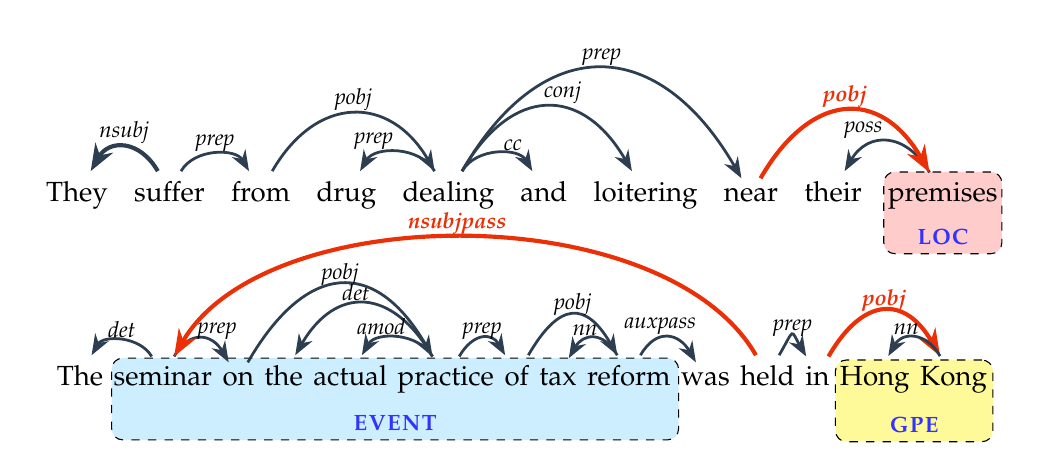
\begin{tikzpicture}[node distance=1.0mm and 1.0mm, >=Stealth, 
		wordnode/.style={draw=none, minimum height=5mm, inner sep=0pt},
		chainLine/.style={line width=1pt,-, color=fontgray},
		entbox/.style={draw=black, rounded corners, fill=red!20, dashed}
		]
		%		\node [word](w1) [] {\footnotesize Ah};
		%		\node [word, right=of w1](w2) [] {\footnotesize ,};
		%		\node [word, right=of w2](w3) [] {\footnotesize today};
		%		\node [word, right=of w3](w4) [] {\footnotesize is};
		\matrix (sent1) [matrix of nodes, nodes in empty cells, execute at empty cell=\node{\strut};]
		{
			They & [1mm]suffer &[1mm]from & [1mm]drug   &  [1mm]  dealing & [1mm]and& [1mm]loitering& [1mm]near & [1mm]their & [1mm]premises\\
			%		 \textbf{\textsc{date}}   &   &   & \textsc{o}     & \textsc{o}   & \textsc{o}  & \textsc{o}& \textsc{event} &  \\
		};
		
		\draw [chainLine, ->, color=fontgray, line width=1.5pt] (sent1-1-2) to [out=120,in=60, looseness=1.4] node[above, yshift=-1mm, color=black]{\footnotesize\it nsubj} (sent1-1-1);
		\draw [chainLine, ->] (sent1-1-2) to [out=60,in=120, looseness=1] node[above, yshift=-1mm, color=black]{\footnotesize\it prep} (sent1-1-3);
		\draw [chainLine, ->] (sent1-1-5) to [out=120,in=60, looseness=1] node[above, yshift=-1mm, xshift=-3mm, color=black]{\footnotesize\it prep} (sent1-1-4);
		\draw [chainLine, ->] (sent1-1-3) to [out=60,in=120, looseness=1.4] node[above, yshift=-1mm, color=black]{\footnotesize\it pobj} (sent1-1-5);
		\draw [chainLine, ->] (sent1-1-5) to [out=60,in=120, looseness=1] node[above, yshift=-1mm, color=black, xshift=2mm]{\footnotesize\it cc} (sent1-1-6);
		\draw [chainLine, ->] (sent1-1-5) to [out=60,in=120, looseness=1.5] node[above, yshift=-1mm, color=black, xshift=2mm]{\footnotesize\it conj} (sent1-1-7);
		\draw [chainLine, ->] (sent1-1-5) to [out=60,in=120, looseness=1.5] node[above, yshift=-1mm, color=black]{\footnotesize\it prep} (sent1-1-8);
		\draw [chainLine, ->, color=fontgray, line width=1pt] (sent1-1-10) to [out=120,in=60, looseness=1.4] node[above, yshift=-1mm, color=black, xshift=-3mm]{\footnotesize\it poss} (sent1-1-9);
		\draw [chainLine, ->, line width=1.5pt, color=myred] (sent1-1-8) to [out=60,in=120, looseness=1.5] node[above, yshift=-1mm, color=myred]{\footnotesize\textit{\textbf{pobj}} } (sent1-1-10);
		
		\begin{pgfonlayer}{background}
		\node [entbox, below=of sent1-1-10, yshift=7mm, text height=8mm, minimum width=15mm] (e1)  [] {\color{blue!80}\textbf{\textsc{loc}}};
		%		\node [entbox, below=of sent1-1-8, xshift=5mm, yshift=6.1mm, text height=8mm, minimum width=18mm, fill=yellow!40] (e2)  [] {\color{blue!80}\textbf{\textsc{Event}}};
		\end{pgfonlayer}
		
		
		
		\matrix (sent2) [matrix of nodes, nodes in empty cells, execute at empty cell=\node{\strut};, below=of sent1, yshift=-14mm]
		{
			The &[-1mm] seminar &[-1mm] on &[-1mm] the & [-1mm]actual   &    [-1mm]practice &[-1mm] of & [-1mm]tax& [-1mm]reform & [-1mm]was & [-1mm]held & [-1mm]in &[-1mm] Hong &[-1mm] Kong\\
			%		 \textbf{\textsc{date}}   &   &   & \textsc{o}     & \textsc{o}   & \textsc{o}  & \textsc{o}& \textsc{event} &  \\
		};
		
		\draw [chainLine, ->] (sent2-1-2) to [out=120,in=60, looseness=1] node[above, yshift=-1mm, xshift=0mm,  color=black]{\footnotesize\it det} (sent2-1-1);
		\draw [chainLine, <-] (sent2-1-3) to [out=120,in=60, looseness=1.5] node[above, yshift=-1.5mm,  color=black, xshift=2mm]{\footnotesize\it prep} (sent2-1-2);
		\draw [chainLine, ->] (sent2-1-6) to [out=120,in=60, looseness=1.5] node[above, yshift=-1mm, xshift=-1mm,  color=black]{\footnotesize\it det} (sent2-1-4);
		\draw [chainLine, ->] (sent2-1-6) to [out=120,in=60, looseness=1] node[above, yshift=-1mm, xshift=-2mm,  color=black]{\footnotesize\it amod} (sent2-1-5);
		\draw [chainLine, ->] (sent2-1-3) to [out=60,in=120, looseness=1.6] node[above, yshift=-1.5mm,  color=black]{\footnotesize\it pobj} (sent2-1-6);
		\draw [chainLine, ->] (sent2-1-6) to [out=60,in=120, looseness=1.5] node[above, yshift=-1.5mm,  color=black]{\footnotesize\it prep} (sent2-1-7);
		\draw [chainLine,<-, line width=1pt] (sent2-1-8) to [out=60,in=120, looseness=1.5] node[above, yshift=-1mm, color=black,xshift=-1mm]{\footnotesize\it nn} (sent2-1-9);
		\draw [chainLine, ->] (sent2-1-7) to [out=60,in=120, looseness=1.8] node[above, yshift=-1.5mm,  color=black]{\footnotesize\it pobj} (sent2-1-9);
		
		\draw [chainLine,->, line width=1pt] (sent2-1-9) to [out=60,in=120, looseness=1.5] node[above, yshift=-1mm, color=black,xshift=-1mm]{\footnotesize\it auxpass} (sent2-1-10);
		\draw [chainLine, ->] (sent2-1-11) to [out=60,in=120, looseness=3.0] node[above, yshift=-1.5mm,  color=black]{\footnotesize\it prep} (sent2-1-12);
		
		\draw [chainLine, ->, color=myred, line width=1.5pt] (sent2-1-12) to [out=60,in=120, looseness=1.6] node[above, yshift=-1.5mm,  color=myred]{\footnotesize\textit{\textbf{pobj}}} (sent2-1-14);
		\draw [chainLine, <-] (sent2-1-13) to [out=60,in=120, looseness=1.4] node[above, yshift=-1mm,  color=black, xshift=-1mm]{\footnotesize\it nn} (sent2-1-14);
		
		\draw [chainLine, <-, color=myred, line width=1.5pt] (sent2-1-2) to [out=60,in=120, looseness=0.8] node[above, yshift=-1mm,  color=myred, xshift=-1mm]{\footnotesize\textit{\textbf{nsubjpass}}} (sent2-1-11);
		
		
		\begin{pgfonlayer}{background}
		\node [entbox, below=of sent2-1-5, xshift=5.7mm, yshift=5.8mm, text height=8mm, minimum width=72mm, fill=myblue!20] (e2)  [] {\color{blue!80}\textbf{\textsc{event}}};
		\node [entbox, below=of sent2-1-13, xshift=5mm, yshift=6.5mm, text height=8mm, minimum width=20mm, fill=yellow!40] (e2)  [] {\color{blue!80}\textbf{\textsc{gpe}}};
		\end{pgfonlayer}
		\end{tikzpicture} 
	}
	%	\vspace*{-7.5mm}
	\caption{Example sentences annotated with named entiteis and dependencies in the OntoNotes 5.0 dataset.}
	%	\vspace*{-6mm}
	\label{fig:examples}
\end{figure}


%1	2-	_	LS	LS	_	15	dep	_	_	O
%2	On	_	IN	IN	_	15	prep	_	_	O
%3	the	_	DT	DT	_	6	det	_	_	B-FAC
%4	eastern	_	JJ	JJ	_	6	amod	_	_	I-FAC
%5	ring	_	NN	NN	_	6	nn	_	_	I-FAC
%6	road	_	NN	NN	_	2	pobj	_	_	I-FAC
%7	,	_	,	,	_	15	punct	_	_	O
%8	three	_	CD	CD	_	10	num	_	_	B-CARDINAL
%9	young	_	JJ	JJ	_	10	amod	_	_	O
%10	men	_	NNS	NNS	_	15	nsubj	_	_	O
%11	in	_	IN	IN	_	10	prep	_	_	O
%12	a	_	DT	DT	_	14	det	_	_	O
%13	Lexus	_	NNP	NNP	_	14	nn	_	_	B-ORG
%14	car	_	NN	NN	_	11	pobj	_	_	O
%15	caught	_	VBD	VBD	_	0	root	_	_	O
%16	my	_	PRP$	PRP$	_	17	poss	_	_	O
%17	attention	_	NN	NN	_	15	dobj	_	_	O
%18	.	_	.	.	_	15	punct	_	_	O

%1	Today	_	NN	NN	_	46	nsubjpass	_	_	B-DATE
%2	,	_	,	,	_	46	punct	_	_	O
%3	the	_	DT	DT	_	6	det	_	_	O
%4	"	_	``	``	_	6	punct	_	_	O
%5	'96	_	CD	CD	_	6	num	_	_	B-DATE
%6	seminar	_	NN	NN	_	46	nsubjpass	_	_	B-EVENT
%7	on	_	IN	IN	_	6	prep	_	_	I-EVENT
%8	the	_	DT	DT	_	10	det	_	_	I-EVENT
%9	actual	_	JJ	JJ	_	10	amod	_	_	I-EVENT
%10	practice	_	NN	NN	_	7	pobj	_	_	I-EVENT
%11	of	_	IN	IN	_	10	prep	_	_	I-EVENT
%12	tax	_	NN	NN	_	13	nn	_	_	I-EVENT
%13	reform	_	NN	NN	_	11	pobj	_	_	I-EVENT
%14	and	_	CC	CC	_	13	cc	_	_	I-EVENT
%15	accounting	_	NN	NN	_	16	nn	_	_	I-EVENT
%16	system	_	NN	NN	_	13	conj	_	_	I-EVENT
%17	for	_	IN	IN	_	13	prep	_	_	I-EVENT
%18	imported	_	VBN	VBN	_	20	amod	_	_	I-EVENT
%19	raw	_	JJ	JJ	_	20	amod	_	_	I-EVENT
%20	materials	_	NNS	NNS	_	17	pobj	_	_	I-EVENT
%21	"	_	''	''	_	6	punct	_	_	O
%22	,	_	,	,	_	6	punct	_	_	O
%23	jointly	_	RB	RB	_	24	advmod	_	_	O
%24	sponsored	_	VBN	VBN	_	6	vmod	_	_	O
%25	by	_	IN	IN	_	24	prep	_	_	O
%26	the	_	DT	DT	_	28	det	_	_	B-ORG
%27	Guangdong	_	NNP	NNP	_	28	nn	_	_	I-ORG
%28	Branch	_	NNP	NNP	_	25	pobj	_	_	I-ORG
%29	of	_	IN	IN	_	28	prep	_	_	O
%30	the	_	DT	DT	_	34	det	_	_	B-ORG
%31	China	_	NNP	NNP	_	34	nn	_	_	I-ORG
%32	Trade	_	NNP	NNP	_	33	nn	_	_	I-ORG
%33	Promotion	_	NNP	NNP	_	34	nn	_	_	I-ORG
%34	Council	_	NNP	NNP	_	29	pobj	_	_	I-ORG
%35	and	_	CC	CC	_	28	cc	_	_	O
%36	the	_	DT	DT	_	41	det	_	_	B-ORG
%37	Hong	_	NNP	NNP	_	38	nn	_	_	I-ORG
%38	Kong	_	NNP	NNP	_	41	nn	_	_	I-ORG
%39	Chinese	_	NNP	NNP	_	41	nn	_	_	I-ORG
%40	General	_	NNP	NNP	_	41	nn	_	_	I-ORG
%41	Chamber	_	NNP	NNP	_	28	conj	_	_	I-ORG
%42	of	_	IN	IN	_	41	prep	_	_	I-ORG
%43	Commerce	_	NNP	NNP	_	42	pobj	_	_	I-ORG
%44	,	_	,	,	_	46	punct	_	_	O
%45	was	_	VBD	VBD	_	46	auxpass	_	_	O
%46	held	_	VBN	VBN	_	0	root	_	_	O
%47	in	_	IN	IN	_	46	prep	_	_	O
%48	Guangzhou	_	NNP	NNP	_	47	pobj	_	_	B-GPE
%49	to	_	TO	TO	_	50	aux	_	_	O
%50	introduce	_	VB	VB	_	46	xcomp	_	_	O
%51	visiting	_	VBG	VBG	_	52	amod	_	_	O
%52	businessmen	_	NN	NN	_	50	dobj	_	_	O
%53	from	_	IN	IN	_	52	prep	_	_	O
%54	Hong	_	NNP	NNP	_	55	nn	_	_	B-GPE
%55	Kong	_	NNP	NNP	_	53	pobj	_	_	I-GPE
%56	,	_	,	,	_	55	punct	_	_	O
%57	Macao	_	NNP	NNP	_	55	conj	_	_	B-GPE
%58	and	_	CC	CC	_	55	cc	_	_	O
%59	mainland	_	NN	NN	_	55	conj	_	_	O
%60	to	_	IN	IN	_	50	prep	_	_	O
%61	the	_	DT	DT	_	65	det	_	_	O
%62	three	_	CD	CD	_	65	num	_	_	B-CARDINAL
%63	main	_	JJ	JJ	_	65	amod	_	_	O
%64	policy	_	NN	NN	_	65	nn	_	_	O
%65	adjustments	_	NNS	NNS	_	60	pobj	_	_	O
%66	for	_	IN	IN	_	65	prep	_	_	O
%67	foreign	_	JJ	JJ	_	68	amod	_	_	O
%68	economy	_	NN	NN	_	66	pobj	_	_	O
%69	and	_	CC	CC	_	68	cc	_	_	O
%70	trade	_	NN	NN	_	68	conj	_	_	O
%71	to	_	TO	TO	_	73	aux	_	_	O
%72	be	_	VB	VB	_	73	auxpass	_	_	O
%73	implemented	_	VBN	VBN	_	65	vmod	_	_	O
%74	by	_	IN	IN	_	73	prep	_	_	O
%75	the	_	DT	DT	_	76	det	_	_	O
%76	State	_	NNP	NNP	_	74	pobj	_	_	B-ORG
%77	this	_	DT	DT	_	78	det	_	_	B-DATE
%78	year	_	NN	NN	_	73	tmod	_	_	I-DATE
%79	.	_	.	.	_	46	punct	_	_	O

The first example in Figure \ref{fig:examples} illustrates the relationship between a dependency structure and a named entity. 
Specifically, the word ``{\it premises}'', which is a named entity of type \textsc{loc} (location), is characterized by the incoming arc with label ``{\it pobj}'' (prepositional object). 
This arc reveals a certain level of the semantic role that the word ``{\it premises}'' plays in the sentence. 
Similarly, the two words ``{\it Hong Kong}'' in the second example that form an entity of type \textsc{gpe} are also characterized by a similar dependency arc towards them.

%The syntactic dependencies describe the bilexical relations between the {\it head} (i.e., {\it parent}) and {\it dependent} words in a sentence. 
%The relationships are associated with dependency relations which indicate the nature of the syntactic relation that holds between the two words.
%For example (Figure \ref{fig:examples}), ``{\it Today}'' is the nominal subject ({\it nsubj}) of ``{\it workday}''.
%The dependency relations, such as subject and object, could be good indicators for the presence of named entities and are helpful for improving recall.
%could be helpful for recognizing more entities, which results in a higher recall for named entity recognizer. 
%As we can see from the first example of Figure \ref{fig:examples}, ``{\it premises}'' is a \textsc{Loc} entity associated with the ``{\it pobj}'' (i.e., prepositional object) dependency relation. 
%In the second example, the two entities (i.e., \textsc{Event} and \textsc{Gpe}) form a subtree and the root words of these two subtrees, ``\textit{seminar}'' and ``\textit{Kong}'', are associated with the dependency relation ``\textit{nsubjpass}'' (i.e., passive nominal subject) and ``{\it pobj}'', respectively. 
%In the second example, the two entities (i.e., \textsc{Event} and \textsc{Gpe}) are associated with parent dependencies that are outside the entity boundaries. 
%The corresponding dependency relations are ``\textit{nsubjpass}'' (i.e., passive nominal subject) and ``{\it pobj}'', respectively.
% and ``{\it New Year}'' is an \textsc{Event} entity associated with ``{\it nn}'' (i.e., noun compound modifier) labels. 
%In practice, we also find that more than 50\% of the entities are related to the dependency relation ``\textit{pobj}'', ``\textit{nsubj}'' (nominal subject) and ``\textit{nn}'' (i.e., noun compound modifier) in the OntoNotes dataset. 
%Capturing such correlations between the dependency relations and named entities could improve the performance on the NER task. 
%Besides, we also find that some \textit{grandchild dependencies} (GD)~\cite{koo2010efficient} such as ``(\textit{prep, pobj})'' can be indicators of named entities. 
%For example, the entity word ``\textit{premises}'' is the prepositional object (\textit{pobj}) of ``\textit{near}'' which is a preposition (\textit{prep}) of ``\textit{dealing}''.
%Meanwhile, other dependency relations such as ``\textit{auxpass}'' and ``\textit{neg}'' can also help to identify the words (i.e., ``\textit{was}'') that are non-entity. 


The long-distance dependencies capturing non-local structural information can also be very helpful for the NER task~\cite{finkel2005incorporating}. 
In the second example of Figure \ref{fig:examples}, the long-distance dependency from ``\textit{held}'' to ``\textit{seminar}'' indicates a direct relation ``\textit{nsubjpass}'' (passive subject) between them, which can be used to characterize the existence of an entity. 
However, existing NER models based on linear-chain structures would have difficulties in capturing such long-distance relations (i.e., non-local structures).

One interesting property, as highlighted in the work of \citet{jie2017efficient}, is that most of the entities form subtrees under their corresponding dependency trees. 
In the example of the \textsc{Event} entity in Figure \ref{fig:examples}, the entity itself forms a subtree and the words inside have rich complex dependencies among themselves. 
Exploiting such dependency edges within the subtrees allows a model to capture non-trivial semantic-level interactions between words within long entities.
For example, ``\textit{practice}'' is the prepositional object (\textit{pobj}) of ``\textit{on}'' which is a preposition (\textit{prep}) of ``\textit{seminar}'' in the \textsc{Event} entity. 
Modeling these grandchild dependencies (GD)~\cite{koo2010efficient} requires the model to capture some higher-order long-distance interactions among different words in a sentence.

%The long-distance dependencies which capture non-local structural information can also be beneficial for the NER task~\cite{finkel2005incorporating}. 
%In the second example of Figure \ref{fig:examples}, the long-distance dependency from ``\textit{held}'' to ``\textit{seminar}'' indicates a direct relation ``\textit{nsubjpass}'' (passive subject) between them. 
%Inference on a linear-structure model could be challenging to capture such long-distance relations (i.e., non-local structures). 
%Moreover, the benefits of long-distance dependencies also apply to recognizing long entities. 
%As reported in \citet{jie2017efficient}, most of the entities form subtrees under their corresponding dependency trees. 
%In the example of the \textsc{Event} entity in Figure \ref{fig:examples}, the entity itself forms a subtree and the words inside have long-distance dependencies among themselves, such as the dependency from ``\textit{on}'' to ``\textit{practice}''. 
%The dependency edges within the subtrees allow a model to capture non-local structures for long entities.
%Other than the direct long-distance dependencies, we can also capture the \textit{indirect long-distance} interactions by the  \textit{grandchild dependencies} (GD)~\cite{koo2010efficient} among three words. 
%For example, the \textsc{Loc} entity ``\textit{premises}'' is the prepositional object (\textit{pobj}) of ``\textit{near}'' which is a preposition (\textit{prep}) of ``\textit{dealing}''. 
%Modeling these grandchild dependencies captures indirect long-distance interactions among different words in a sentence.


%Inspired by the above characteristics of dependencies, we aim to build a model that is able to capture the rich structural and semantic information conveyed by the dependency trees.
%In this work, we design a simple and effective dependency-guided model based on the state-of-the-art NER model, LSTM-CRF~\cite{lample2016neural}. 
%Our model is able to capture both contextual information and long-distance interactions for the NER task. 
%Our contributions can be summarized as follows:
%\squishlist
%\item Motivated by the relations between dependencies and named entities. 
%We propose a simple and effective dependency-guided LSTM-CRF to encode the dependency tree structures for improving the performance of NER. 
%\item Through extensive experiments on several datasets from four languages, we demonstrate the effectiveness of applying dependency trees to NER and achieve state-of-the-art performance.
%\item Additional experiments show that  the improvement also applies to low-resource NER. Our further analysis shows strong correlations between the performance improvements and the dependency trees (i.e., dependency relations and long-distance interactions). 
%\squishend

Inspired by the above characteristics of dependency structures, in this work, we propose a simple yet effective dependency-guided model for NER. 
Our neural network based model is able to capture both contextual information and rich long-distance interactions between words for the NER task. 
Through extensive experiments on several datasets on different languages, we demonstrate the effectiveness of our model, which achieves the state-of-the-art performance. 
To the best of our knowledge, this is the first work that leverages the complete dependency graphs for NER.
%We make our code publicly available at \url{http://www.statnlp.org/research/information-extraction}.


\section{Related Work}
NER has been a long-standing task in the field of NLP. 
While many recent works~\cite{peters2018deep,akbik2018coling,devlin2019bert} focus on finding good contextualized word representations for improving NER, our work is mostly related to the literature that focuses on employing dependency trees for improving NER. 


\citet{sasano2008japanese} exploited the syntactic dependency features for Japanese NER and achieved improved performance with a support vector machine~(SVM)~\cite{cortes1995support} classifier. 
Similarly, \citet{ling2012fine} included the head word in a dependency edge as features for fine-grained entity recognition. 
Their approach is a pipeline where they extract the entity mentions with  linear-chain conditional random fields~(CRF)~\cite{lafferty2001conditional} and used a classifier to predict the entity type.
%then classify the mentions into multiple entity labels. 
\citet{liu2010recognizing} proposed to link the words that are associated with selected typed dependencies (e.g., ``{\it nn}'', ``{\it prep}'') using a skip-chain CRF~\cite{sutton2004collective} model. 
They showed that some specific relations between the words can be exploited for improved NER. 
%As the underlying model involves loopy structures, exact inference is not available. 
%As the underlying model involves loopy structures, they performed inexact inference.
\citet{cucchiarelli2001unsupervised} applied a dependency parser to obtain the syntactic relations for the purpose of unsupervised NER. 
The resulting relation information serves as the features for potential existence of named entities. 
\citet{jie2017efficient} proposed an efficient dependency-guided model based on the semi-Markov CRF~\cite{sarawagi2004semi} for NER. 
The purpose is to reduce time complexity while maintaining the non-Markovian features.
%in the model. 
% properties of semi-Markov CRF. 
They observed certain relationships between the dependency edges and the named entities. 
Such relationships are able to define a reduced search space for their model. 
While these previous approaches do not make full use of the dependency tree structures, we focus on exploring neural architectures to exploit the  complete structural information conveyed by the dependency trees.
% dependency trees including the dependency relations. 

%Other than dependency trees, NER can also be benefited from other linguistics structures like parse trees, which are more expensive in terms of annotation costs compared to the dependency trees.  
%\citet{finkel2009joint} proposed a CRF-CFG model for joint parsing and named entity recognition. 
%Their model achieved competitive performance on the OntoNotes dataset~\cite{pradhan2013towards}. 
%\citet{li2017leveraging} applied the recursive neural network on top of the parse tree structures and obtained state-of-the-art performance on the OntoNotes dataset.


%We further analyze the useful dependency patterns for 


\section{Model}

Our dependency-guided model is based on the state-of-the-art BiLSTM-CRF model proposed by \citet{lample2016neural}.
% as it leverages the contextual representations which play an important role in the NER task. 
We first briefly present their model  as background and next present our dependency-guided model.
%and extended it to the dependency-guided models. 


\subsection{Background: BiLSTM-CRF}
In the task of named entity recognition, we aim to predict the label sequence $\vec{y} = \{y_1, y_2,\cdots, y_n\}$ given the input sentence $\vec{x}=\{x_1, x_2, \cdots, x_n\}$ where $n$ is the number of words.
%with $n$ words. 
The labels in $\vec{y}$ are defined by a label set with the standard \textsc{iobes}\footnote{``\textsc{s-}'' indicates the entity with a single word and ``\textsc{e-}'' indicates the end of an entity.} labeling scheme~\cite{ramshaw1999text,ratinov2009design}. 
The CRF~\cite{lafferty2001conditional} layer defines the probability of the label sequence $\vec{y}$ given $\vec{x}$:
\begin{equation}
P(\vec{y} \vert \vec{x})
=
\frac
{\exp ( score(\vec{x}, \vec{y})  )  }
{\sum_{\vec{y}^\prime }\exp ( score(\vec{x}, \vec{y}^\prime) )  }
\end{equation}
%\begin{center}
%	\begin{tabular}{c}
%		$
%		P(\vec{y} \vert \vec{x})
%		=
%		\frac
%		{\exp ( score(\vec{x}, \vec{y})  )  }
%		{\sum_{\vec{y}^\prime }\exp ( score(\vec{x}, \vec{y}^\prime) )  }
%		$
%	\end{tabular}
%	%\vspace{-2mm}
%\end{center}

Following \citet{lample2016neural}, the score is defined as the sum of transitions and emissions from the bidirectional LSTM (BiLSTM): 
\begin{equation}
score(\vec{x} , \vec{y}) = \sum_{i=0}^n A_{y_i, y_{i+1}} + \sum_{i=1}^n F_{\vec{x}, y_i}
\end{equation}
%\begin{center}
%	\begin{tabular}{c}
%		$
%		score(\vec{x} , \vec{y}) = \sum\limits_{i=0}^n A_{y_i, y_{i+1}} + \sum\limits_{i=1}^n F_{\vec{x}, y_i}
%		$
%	\end{tabular}
%	%\vspace{-2mm}
%\end{center}
where $\mathbf{A}$ is a transition matrix in which $A_{y_i, y_{i+1}}$ is the transition parameter from the label $y_i$ to the label $y_{i+1}$\footnote{$y_0$ and $y_{n+1}$ are \texttt{start} and \texttt{end} labels.}. 
$\mathbf{F}_\vec{x}$ is an emission matrix where $F_{\vec{x}, y_i}$ represents the scores of the label  $y_i$ at the $i$-th position. 
Such scores are provided by the parameterized LSTM~\cite{hochreiter1997long} networks. 
During training, we minimize the negative log-likelihood to obtain the model parameters including both LSTM and transition parameters. 
%During training, we minimize the The model parameters can be obtained by minimizing the negative log-likelihood.



\subsection{Dependency-Guided LSTM-CRF}
\paragraph{Input Representations}
The word representation $\vec{w}$ in the BiLSTM-CRF~\cite{lample2016neural,ma2016end,D17-1035} model consists of the concatenation of the word embedding as well as the corresponding character-based representation. 
Inspired by the fact that each word (except the root) in a sentence has exactly one \textit{head} (i.e., \textit{parent}) word in the dependency structure, we can enhance the word representations with such dependency information. 
%Specifically, the head word embeddings and dependency relation embeddings can be included as part to the word representation. 
Similar to the work by \citet{miwa2016end}, we concatenate the word representation together with the corresponding head word representation and dependency relation embedding as the input representation. 
Specifically, given a dependency edge $(x_h, x_i, r)$ with $x_h$ as parent, $x_i$ as child and $r$ as dependency relation, the representation at position $i$ can be denoted as:
\begin{equation}
\vec{u}_i = \left [
\vec{w}_i; \vec{w}_h; \vec{v}_{r}	
\right ], ~~ x_h = parent(x_i)
\label{equ:rep}
\end{equation}
%\begin{center}
%	\begin{tabular}{c}
%		$
%		\vec{u}_i = \left [
%		\vec{w}_i; \vec{w}_h; \vec{v}_{r}	
%		\right ], ~~ x_h = parent(x_i)
%		$
%	\end{tabular}
%	%\vspace{-2mm}
%\end{center}
where $\vec{w}_i$ and $\vec{w}_h$ are the word representations of the word $x_i$ and its parent $x_h$, respectively. 
%$\vec{w}_i$ is the concatenation of pre-trained word embeddings (e.g. Glove~\cite{pennington2014glove}) of $x_i$ and its character-based representation. 
We take the final hidden state of character-level BiLSTM as the character-based representation~\cite{lample2016neural}.
%Following state-of-the-art neural architectures~\cite{lample2016neural,ma2016end,D17-1035}, a word representation is the concatenation of pre-trained word embeddings (e.g. Glove~\cite{pennington2014glove}) and its character-based word presentation $\vec{c}_i$. 
$\vec{v}_r$ is the embedding for the dependency relation $r$. 
These relation embeddings are randomly initialized and fine-tuned during training. 
The above representation allows us to capture the direct long-distance interactions at the input layer. 
For the word that is a root of the dependency tree, we treat its parent as itself\footnote{We also tried using a root word embedding but the performance is similar.} and create a root relation embedding. 
Additionally, contextualized word representations (e.g., ELMo) can also be concatenated into $\vec{u}$.

\begin{figure}[t!]
	\centering
	\adjustbox{max width=1\linewidth}{
		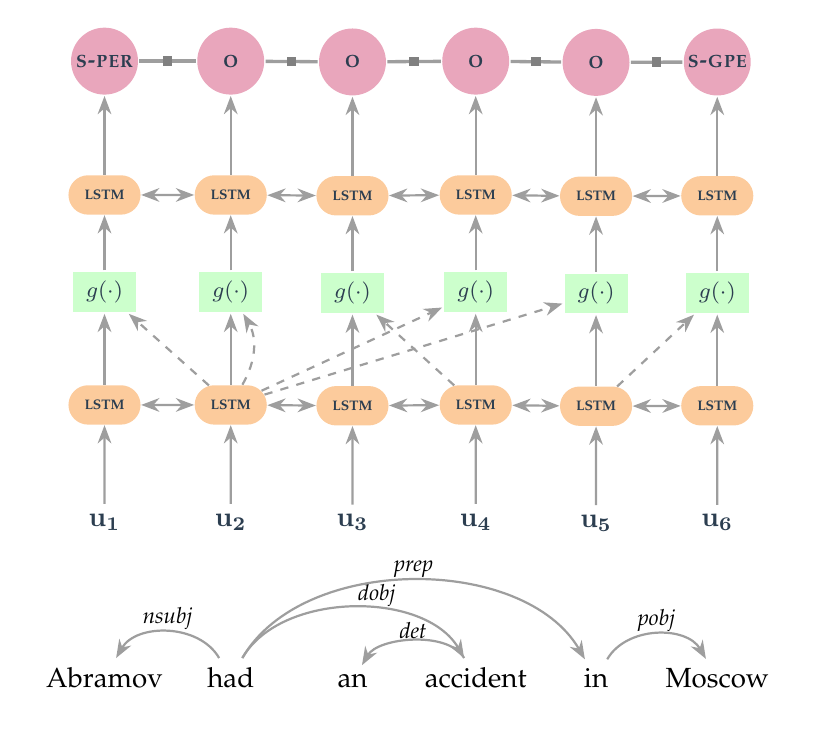
\begin{tikzpicture}[node distance=10.0mm and 12mm, >=Stealth, 
		sentity/.style={draw=none, circle, minimum height=8.5mm, minimum width=8.5mm,line width=1pt, inner sep=0pt, fill=purple!35},
		lstm/.style={draw=none, minimum height=5mm, rounded rectangle, fill=puffin!50, minimum width=11.5mm, label={center:\tiny \textcolor{fontgray}{\bf LSTM}}},
		%		, blur shadow={shadow blur steps=5}
		plus/.style={draw=none, minimum height=3mm, circle, fill={rgb:red,0;green,210;blue,211}, label={center:\footnotesize \textcolor{white}{+}}},
		gfunc/.style={draw=none, minimum height=5mm, rectangle, fill=green!20, label={center:\footnotesize \textcolor{fontgray}{$g(\cdot)$}}, minimum width=8mm, line width = 1.5pt},
		emb/.style={draw=none, minimum height=3mm, rounded rectangle, fill=none, minimum width=12mm, text=fontgray},
		%		cyan!40
		chainLine/.style={line width=0.8pt,->, color=mygray},
		%	background rectangle/.style={fill=olive!45}, show background rectangle, 
		%		line width=1.3pt
		]
		
		
		\matrix (s) [matrix of nodes, nodes in empty cells, execute at empty cell=\node{\strut};]
		{
			Abramov & [2ex]had & [5ex]an & [3ex]accident   &   [3ex] in  & [3ex] Moscow\\
			%		 \textbf{\textsc{date}}   &   &   & \textsc{o}     & \textsc{o}   & \textsc{o}  & \textsc{o}& \textsc{event} &  \\
		};
		
		\draw [chainLine, ->] (s-1-2) to [out=120,in=60, looseness=1] node[above, yshift=-1mm, color=black]{\footnotesize\it nsubj} (s-1-1);
		\draw [chainLine, ->] (s-1-4) to [out=120,in=60, looseness=0.8] node[above, yshift=-1mm, color=black]{\footnotesize\it det} (s-1-3);
		\draw [chainLine, ->] (s-1-2) to [out=60,in=120, looseness=0.9] node[above, yshift=-1.2mm, xshift=3mm, color=black]{\footnotesize\it dobj} (s-1-4);
		\draw [chainLine, ->] (s-1-2) to [out=60,in=120, looseness=0.9] node[above, yshift=-1mm, color=black]{\footnotesize\it prep} (s-1-5);
		\draw [chainLine, ->] (s-1-5) to [out=60,in=120, looseness=1] node[above, yshift=-1mm, color=black]{\footnotesize\it pobj} (s-1-6);
		
		\node[emb, above= of s-1-1, yshift=5mm] (u1) {$\vec{u}_\mathbf{1}$};
		\node[emb, above= of s-1-2, yshift=5mm] (u2) {$\vec{u}_\mathbf{2}$};
		\node[emb, above= of s-1-3, yshift=5.8mm] (u3) {$\vec{u}_\mathbf{3}$};
		\node[emb, above= of s-1-4, yshift=5mm] (u4) {$\vec{u}_\mathbf{4}$};
		\node[emb, above= of s-1-5, yshift=5mm] (u5) {$\vec{u}_\mathbf{5}$};
		\node[emb, above= of s-1-6, yshift=5mm] (u6) {$\vec{u}_\mathbf{6}$};
		
		\node[lstm, above= of u1] (h1) {};
		\node[lstm, above=of u2](h2) {};
		\node[lstm, above= of u3](h3) {};
		\node[lstm, above= of u4](h4) {};
		\node[lstm, above= of u5](h5) {};
		\node[lstm, above= of u6](h6) {};
		
		
		
		\node[gfunc, above= of h1, yshift=-1mm] (g1) {};
		\node[gfunc, above=of h2, yshift=-1mm](g2) {};
		\node[gfunc, above= of h3, yshift=-1mm](g3) {};
		\node[gfunc, above= of h4, yshift=-1mm](g4) {};
		\node[gfunc, above= of h5, yshift=-1mm](g5) {};
		\node[gfunc, above= of h6, yshift=-1mm](g6) {};
		
		\node[lstm, above= of g1, yshift=-3mm] (m1) {};
		\node[lstm, above=of g2, yshift=-3mm](m2) {};
		\node[lstm, above= of g3, yshift=-3mm](m3) {};
		\node[lstm, above= of g4, yshift=-3mm](m4) {};
		\node[lstm, above= of g5, yshift=-3mm](m5) {};
		\node[lstm, above= of g6, yshift=-3mm](m6) {};
		
		%		\node[left = of m1, xshift](layer1) {$L=1$};
		
		\node[sentity, above= of m1] (e1) {\footnotesize \textcolor{fontgray}{\bf \textsc{s-per}}};
		\node[sentity, above=of m2](e2) {\footnotesize \textcolor{fontgray}{\bf \textsc{o}}};
		\node[sentity, above= of m3](e3) {\footnotesize \textcolor{fontgray}{\bf \textsc{o}}};
		\node[sentity, above= of m4](e4) {\footnotesize \textcolor{fontgray}{\bf \textsc{o}}};
		\node[sentity, above= of m5](e5) {\footnotesize \textcolor{fontgray}{\bf \textsc{o}}};
		\node[sentity, above= of m6](e6) {\footnotesize \textcolor{fontgray}{\bf \textsc{s-gpe}}};
		
		
		\draw [chainLine] (u1) to (h1);
		\draw [chainLine] (u2) to (h2);
		\draw [chainLine] (u3) to (h3);
		\draw [chainLine] (u4) to (h4);
		\draw [chainLine] (u5) to (h5);
		\draw [chainLine] (u6) to (h6);
		
		\draw [chainLine] (h1) to  (g1);
		\draw [chainLine] (h2) to (g2);
		\draw [chainLine] (h3) to (g3);
		\draw [chainLine] (h4) to (g4);
		\draw [chainLine] (h5) to (g5);
		\draw [chainLine] (h6) to (g6);
		
		\draw [chainLine] (g1) to (m1);
		\draw [chainLine] (g2) to (m2);
		\draw [chainLine] (g3) to (m3);
		\draw [chainLine] (g4) to (m4);
		\draw [chainLine] (g5) to (m5);
		\draw [chainLine] (g6) to (m6);
		
		\draw [chainLine] (m1) to  (e1);
		\draw [chainLine] (m2) to   (e2);
		\draw [chainLine] (m3) to   (e3);
		\draw [chainLine] (m4) to    (e4);
		\draw [chainLine] (m5) to   (e5);
		\draw [chainLine] (m6) to   (e6);
		
		\draw [chainLine, dashed] (h2) to  [out=60,in=-60] (g2);
		\draw [chainLine, dashed] (h2) to (g1);
		\draw [chainLine, dashed] (h2) to (g4);
		\draw [chainLine, dashed] (h2) to (g5);
		\draw [chainLine, dashed] (h4) to (g3);
		\draw [chainLine, dashed] (h5) to (g6);
		
		\draw [chainLine, <->] (h1) to (h2);
		\draw [chainLine, <->] (h2) to (h3);
		\draw [chainLine, <->] (h3) to (h4);
		\draw [chainLine, <->] (h4) to (h5);
		\draw [chainLine, <->] (h5) to (h6);
		
		\draw [chainLine, <->] (m1) to (m2);
		\draw [chainLine, <->] (m2) to (m3);
		\draw [chainLine, <->] (m3) to (m4);
		\draw [chainLine, <->] (m4) to (m5);
		\draw [chainLine, <->] (m5) to (m6);
		
		\draw [chainLine, line width=1.2pt, -, middlefactor] (e1) to (e2);
		\draw [chainLine, line width=1.2pt, -, middlefactor] (e2)to (e3);
		\draw [chainLine, line width=1.2pt, -, middlefactor] (e3)to (e4);
		\draw [chainLine, line width=1.2pt, -, middlefactor]  (e4)to (e5);
		\draw [chainLine, line width=1.2pt, -, middlefactor] (e5)to (e6);
		
		\end{tikzpicture} 
	}
	%	\vspace*{-9mm}
	\caption{Dependency-guided LSTM-CRF with 2 LSTM Layers. Dashed connections mimic the dependency edges. ``$g(\cdot)$'' represents the interaction function.}
	%	\vspace*{-5mm}
	\label{fig:model2layer}
\end{figure}

%1	Abramov	_	NNP	NNP	_	2	nsubj	_	_	B-PERSON
%2	had	_	VBD	VBD	_	0	root	_	_	O
%3	a	_	DT	DT	_	5	det	_	_	O
%4	car	_	NN	NN	_	5	nn	_	_	O
%5	accident	_	NN	NN	_	2	dobj	_	_	O
%6	in	_	IN	IN	_	2	prep	_	_	O
%7	Moscow	_	NNP	NNP	_	6	pobj	_	_	B-GPE
%8	last	_	JJ	JJ	_	9	amod	_	_	B-TIME
%9	night	_	NN	NN	_	2	tmod	_	_	I-TIME
%10	and	_	CC	CC	_	2	cc	_	_	O
%11	was	_	VBD	VBD	_	13	auxpass	_	_	O
%12	seriously	_	RB	RB	_	13	advmod	_	_	O
%13	injured	_	VBN	VBN	_	2	conj	_	_	O
%14	.	_	.	.	_	2	punct	_	_	O


\paragraph{Neural Architecture}
Given the dependency-encoded input representation $\vec{u}$, we apply the LSTM to capture the contextual information and model the interactions between the words and their corresponding parents in the dependency trees. 
%use dependencies to provide long-distance interactions guidance. 
Figure \ref{fig:model2layer} shows the proposed dependency-guided LSTM-CRF (\textbf{DGLSTM-CRF}) with 2 LSTM layers for the example sentence ``\textit{Abramov had an accident in Moscow}'' and its dependency structure. 
%Figure \ref{fig:model2layer} shows the overall dependency-guided LSTM-CRF ($\textbf{DGLSTM-CRF}$) model architecture given the example sentence ``\textit{Abramov had an accident in Moscow}'' and its dependency structure. 
The corresponding label sequence is \{\textsc{s-per}, \textsc{o}, \textsc{o}, \textsc{o}, \textsc{o}, \textsc{s-gpe}\}. 
%Followed by the first BiLSTM, the hidden states at each position will propagate to the next BiLSTM layer and propagate to its child following the dependency trees. 
Followed by the first BiLSTM, the hidden states at each position will propagate to the next BiLSTM layer and its child along the dependency trees. 
For example, the hidden state of the word ``\textit{had}'', $\vec{h}_2^{(1)}$, will propagate to its child ``\textit{Abramov}'' at the first position. 
For the word that is root, the hidden state at that specific position will propagate to itself. 
We use an \textit{interaction function} $g(\vec{h}_i, \vec{h}_{p_i})$ to capture the interaction between the child and its parent in a dependency. 
Such an interaction function can be concatenation, addition or a  multilayer perceptron (MLP). 
We further apply another BiLSTM layer on top of the interaction functions to produce the context representation for the final CRF layer. 

The architecture shown in Figure \ref{fig:model2layer} with a 2-layer BiLSTM can effectively encode the grandchild dependencies because the input representations encode the parent information and the interaction function further propagate the grandparent information. 
Such propagations allow the model to capture the indirect long-distance interactions from the grandchild dependencies between the words in the sentence as mentioned in Section \ref{sec:intro}. 
In general, we can stack more interaction functions and BiLSTMs to enable deeper reasoning over the dependency trees. 
%Following the dependency structure, we can obtain the representation $\vec{u}$ at each position (Equation \ref{equ:rep}).
%However, 1-layer LSTM may not be able to capture the grandchild dependencies, which are statistically related to named entity as mentioned Section \ref{sec:intro}. 
%The grandchild dependencies can capture longer interactions between the words in the sentence.
%The grandparent of an entity component could be part of the entity or has a direct relation to this entity. 
%To enable such interactions, we stack multiple layers of LSTMs and guide the flow of the representations to there parents at next layer. 
Specifically, the hidden states of the $(l+1)$-th layer $\mathbf{H}^{(l+1)}$ can be calculated from the hidden state of the previous layer $\mathbf{H}^{(l)}$:
\begin{equation}
\begin{split}
\mathbf{H}^{(l+1)} & \!   = \!\text{BiLSTM}
\Big ( 
f \big (\mathbf{H}^{(l)} \big )
\Big ) \\
\mathbf{H}^{(l)} & \! = \!\!
\left [
\vec{h}_1^{(l)}, \vec{h}_2^{(l)}, \cdots, \vec{h}_n^{(l)}
\right ] \\
f\big (\mathbf{H}^{(l)} \big ) &\!  = \!\!
\Big [
g (
\vec{h}_1^{(l)}, \vec{h}_{p_1}^{(l)}
), 
\cdots ,
g (
\vec{h}_n^{(l)},\vec{h}_{p_n}^{(l)}
)
\Big ]
\end{split}\nonumber
\end{equation}
%\begin{equation}
%\begin{split}
%\mathbf{H}^{(l+1)} & \!   = \!\text{BiLSTM}
%\Big ( 
%f \big (\mathbf{H}^{(l)} \big )
%\Big ) \\
%\mathbf{H}^{(l)} & \! = \!\!
%\left [
%\vec{h}_1^{(l)}, \vec{h}_2^{(l)}, \cdots, \vec{h}_n^{(l)}
%\right ] \\
%f\big (\mathbf{H}^{(l)} \big ) &\!  = \!\!
%\Big [
%   g (
%      \vec{h}_1^{(l)}, \vec{h}_{p_1}^{(l)}
%   ), 
%   \cdots ,
%  g (
%   \vec{h}_n^{(l)},\vec{h}_{p_n}^{(l)}
%   )
%\Big ]
%\end{split}\nonumber
%\end{equation}
where $p_i$ indicates the parent index of the word $x_i$. 
$g(\vec{h}_i^{(l)}, \vec{h}_{p_i}^{(l)})$ represents the interaction functions between the hidden state at the $i$-th and  $p_i$-th positions under the dependency edges $(x_{p_i}, x_i)$. 
%The interaction function is similar to the concept in 
%At the output of the first-layer LSTM in Figure \ref{fig:model2layer}, we concatenate the hidden state at position $i$ and the hidden state of its parent to make a new representation, which will be the input representation to the next layer. 
The number of layers $L$ can be chosen according to the performance on the development set. 



\paragraph{Interaction Function}
The interaction function between the parent and child representations can be defined in various ways. 
Table \ref{tab:interfunc} shows the list of interaction function considered in our experiments. 
The first one returns the hidden state itself, which is equivalent to stacking the LSTM layers. 
%We investigate the following functions in the underlying model:
%\begin{equation}
%g(\vec{h}_i, \vec{h}_{p_i}) = 
%\left\{
%\begin{matrix}
%\vec{h}_i &  \! \!\!\!  \text{Self}\\ 
%\vec{h}_c \bigoplus  \vec{h}_p &  \! \!\!\!  \text{Concatenation}\\ 
%\vec{h}_c +  \vec{h}_p & \! \!\!\!  \text{Addition}\\ 
%\sigma \big (\mathbf{W}_1\vec{h}_c \! + \! \mathbf{W}_2\vec{h}_p \big ) & \!\! \!\!  \text{MLP} \\
%\end{matrix}\right.
%\nonumber
%\end{equation}
\begin{table}[h!]
	\centering
	\scalebox{1}{
		\begin{tabular}{ll}
			\toprule
			\textbf{Interaction Function}& $g(\vec{h}_i, \vec{h}_{p_i}) $ \\
			\midrule
			Self connection & $\vec{h}_i$\\
			Concatenation & $\vec{h}_i \bigoplus  \vec{h}_{p_i}$\\
			Addition & $\vec{h}_i +  \vec{h}_{p_i}$\\
			MLP & $\text{ReLU} \big (\mathbf{W}_1\vec{h}_i \! + \! \mathbf{W}_2\vec{h}_{p_i} \big )$ \\
			\bottomrule
		\end{tabular}
	}
	%	\vspace*{-3mm}
	\caption{List of interaction functions.}
	%	\vspace*{-4mm}
	\label{tab:interfunc}
\end{table}
The concatenation and addition involve no parameter, which are straightforward ways to model the interactions. 
The last one applies an MLP to model the interaction between parent and child representations. 
%The interaction function $g(\vec{h}_c, \vec{h}_p)$ can take one of these 3 operations. 
%Specifically, the first two operations are intuitive and no parameter involve. 
%The last one is applying an MLP to model the interactions between parent and child representations. 
%$\sigma$ is the non-linear activation function. 
With the rectified linear unit (ReLU) as activation function, the $g(\vec{h}_i, \vec{h}_{p_i})$ function is analogous to a graph convolutional network (GCN)~\cite{kipf2017semi} formulation. 
In such a graph, each node has a self connection (i.e., $\vec{h}_i$) and a dependency connection with parent (i.e., $\vec{h}_{p_i}$).  
Similar to the work by \citet{marcheggiani2017encoding}, we adopt different parameters $\mathbf{W}_1$ and $\mathbf{W}_2$ for self and dependency connections. 
%Such interaction function can be regarded as a graph where each node has only a self connection and a dependency connection. 
%The connections are parameterized by a different weight matrix $\mathbf{W}_1$ and $\mathbf{W}_2$. 
% becomes a layer of graph convolutional networks~(GCN)~\cite{kipf2017semi}. 
%Following \citet{kipf2017semi,zhang2018graph}, the hidden state of the $i^{th}$ node can be calculated by:
%\begin{equation}
%\vec{h}_i
%=
%\text{ReLU}
%\Big(
%\sum_{j=1}^{n}
%A_{ij}
%\mathbf{W} \vec{h}_j
%\Big)
%\end{equation}
%where $\mathbf{W}$ is the model parameter. 
%$\mathbf{A}$ is an $n\times n$ adjacency matrix where $A_{ij} = 1$ indicates a connection from the $i^{th}$ node to the $j^{th}$ node. 
%To propagate the information from previous layer to next layer, we usually have $A_{ii} = 1$ for all $i$. 
%In our case, $A_ij = 1$ only when $i=j$ or the $j^{th}$ word is the parent of the $i^{th}$ word. 
%Thus, there are only two terms under this summation. 
%In this case, the interaction function can be interpreted as a GCN layer. 

%\begin{figure}[t!]
%	\centering
%	\adjustbox{max width=1\linewidth}{
%		\begin{tikzpicture}[node distance=6.0mm and 10mm, >=Stealth, 
%		sentity/.style={draw=none, circle, minimum height=8.5mm, minimum width=8.5mm,line width=1pt, inner sep=0pt, fill=purple!65, blur shadow={shadow blur steps=5}},
%		lstm/.style={draw=none, minimum height=5mm, rounded rectangle, fill=puffin, minimum width=11.5mm, label={center:\tiny \textcolor{white}{\bf LSTM}}, blur shadow={shadow blur steps=5}},
%		relu/.style={draw=none, minimum height=5mm, rectangle, fill=green!20, label={center:\footnotesize \textcolor{fontgray}{\bf ReLU}}, minimum width=12mm, line width = 1.5pt},
%		emb/.style={draw=none, minimum height=3mm, rounded rectangle, fill=cyan, minimum width=12mm, text=white},
%		chainLine/.style={line width=0.8pt,->, color=mygray},
%		%	background rectangle/.style={fill=olive!45}, show background rectangle, 
%		%		line width=1.3pt
%		]
%		
%		
%		\matrix (s) [matrix of nodes, nodes in empty cells, execute at empty cell=\node{\strut};]
%		{
%			Abramov & [2ex]had & [5ex]an & [3ex]accident   &   [3ex] in  & [3ex] Moscow\\
%			%		 \textbf{\textsc{date}}   &   &   & \textsc{o}     & \textsc{o}   & \textsc{o}  & \textsc{o}& \textsc{event} &  \\
%		};
%		
%		\draw [chainLine, ->] (s-1-2) to [out=120,in=60, looseness=1] node[above, yshift=-1mm, color=black]{\footnotesize\it nsubj} (s-1-1);
%		\draw [chainLine, ->] (s-1-4) to [out=120,in=60, looseness=0.8] node[above, yshift=-1mm, color=black]{\footnotesize\it det} (s-1-3);
%		\draw [chainLine, ->] (s-1-2) to [out=60,in=120, looseness=0.9] node[above, yshift=-1.2mm, xshift=3mm, color=black]{\footnotesize\it dobj} (s-1-4);
%		\draw [chainLine, ->] (s-1-2) to [out=60,in=120, looseness=0.9] node[above, yshift=-1mm, color=black]{\footnotesize\it prep} (s-1-5);
%		\draw [chainLine, ->] (s-1-5) to [out=60,in=120, looseness=1] node[above, yshift=-1mm, color=black]{\footnotesize\it pobj} (s-1-6);
%		
%		\node[emb, above= of s-1-1, yshift=9mm] (u1) {$\vec{h}_\mathbf{1}$};
%		\node[emb, above= of s-1-2, yshift=9mm] (u2) {$\vec{h}_\mathbf{2}$};
%		\node[emb, above= of s-1-3, yshift=9.8mm] (u3) {$\vec{h}_\mathbf{3}$};
%		\node[emb, above= of s-1-4, yshift=9mm] (u4) {$\vec{h}_\mathbf{4}$};
%		\node[emb, above= of s-1-5, yshift=9mm] (u5) {$\vec{h}_\mathbf{5}$};
%		\node[emb, above= of s-1-6, yshift=9mm] (u6) {$\vec{h}_\mathbf{6}$};
%		
%%		\node[lstm, above= of u1] (h1) {};
%%		\node[lstm, above=of u2](h2) {};
%%		\node[lstm, above= of u3](h3) {};
%%		\node[lstm, above= of u4](h4) {};
%%		\node[lstm, above= of u5](h5) {};
%%		\node[lstm, above= of u6](h6) {};
%		
%		
%		
%		\node[relu, above= of h1, yshift=-2mm] (g1) {};
%		\node[relu, above=of h2, yshift=-2mm](g2) {};
%		\node[relu, above= of h3, yshift=-2mm](g3) {};
%		\node[relu, above= of h4, yshift=-2mm](g4) {};
%		\node[relu, above= of h5, yshift=-2mm](g5) {};
%		\node[relu, above= of h6, yshift=-2mm](g6) {};
%		
%%		\node[lstm, above= of g1, yshift=-3mm] (m1) {};
%%		\node[lstm, above=of g2, yshift=-3mm](m2) {};
%%		\node[lstm, above= of g3, yshift=-3mm](m3) {};
%%		\node[lstm, above= of g4, yshift=-3mm](m4) {};
%%		\node[lstm, above= of g5, yshift=-3mm](m5) {};
%%		\node[lstm, above= of g6, yshift=-3mm](m6) {};
%		
%		\node[sentity, above= of g1] (e1) {\footnotesize \textcolor{white}{\bf \textsc{s-per}}};
%		\node[sentity, above=of g2](e2) {\footnotesize \textcolor{white}{\bf \textsc{o}}};
%		\node[sentity, above= of g3](e3) {\footnotesize \textcolor{white}{\bf \textsc{o}}};
%		\node[sentity, above= of g4](e4) {\footnotesize \textcolor{white}{\bf \textsc{o}}};
%		\node[sentity, above= of g5](e5) {\footnotesize \textcolor{white}{\bf \textsc{o}}};
%		\node[sentity, above= of g6](e6) {\footnotesize \textcolor{white}{\bf \textsc{s-gpe}}};
%		
%		
%		
%
%%		
%%		\draw [chainLine] (g1) to (m1);
%%		\draw [chainLine] (g2) to (m2);
%%		\draw [chainLine] (g3) to (m3);
%%		\draw [chainLine] (g4) to (m4);
%%		\draw [chainLine] (g5) to (m5);
%%		\draw [chainLine] (g6) to (m6);
%		
%		\draw [chainLine] (g1) to (e1);
%		\draw [chainLine] (g2) to (e2);
%		\draw [chainLine] (g3) to (e3);
%		\draw [chainLine] (g4) to (e4);
%		\draw [chainLine] (g5) to (e5);
%		\draw [chainLine] (g6) to (e6);
%		
%%		\draw [chainLine] (h2) to  [out=60,in=-60] (g2);
%		\draw [chainLine] (u2) to (g1);
%		\draw [chainLine] (u1) to (g2);
%		\draw [chainLine] (u2) to (g4);
%		\draw [chainLine] (u4) to (g2);
%		\draw [chainLine] (u2) to (g5);
%		\draw [chainLine] (u5) to (g2);
%		\draw [chainLine] (u4) to (g3);
%		\draw [chainLine] (u3) to (g4);
%		\draw [chainLine] (u5) to (g6);
%		\draw [chainLine] (u6) to (g5);
%		
%		\draw [chainLine] (u1) to (g1);
%		\draw [chainLine] (u2) to (g2);
%		\draw [chainLine] (u3) to (g3);
%		\draw [chainLine] (u4) to (g4);
%		\draw [chainLine] (u5) to (g5);
%		\draw [chainLine] (u6) to (g6);
%		
%		
%		\draw [chainLine, line width=1.2pt, -] (e1) to (e2)to (e3)to (e4)to (e5)to (e6);
%		
%		\end{tikzpicture} 
%	}
%	\caption{Dependency-guided GCNs with 1 GCN layer.}
%	\label{fig:modelgcn}
%\end{figure}

%\subsection{Dependency-Guided GCNs}
%Encoding dependency trees with graph convolutional networks~\cite{kipf2017semi} has been widely studied in a variety of NLP applications, such as relation extraction~\cite{zhang2018graph} and semantic role labeling~\cite{marcheggiani2017encoding}. 
%Dependency relation information is not well-considered since it does not have significant impact on their tasks. 
%However, dependency labels can serve as the indicator of entities as mentioned in Section \ref{sec:intro}. 
%Given a graph with $n$ nodes, we can represent the graph with an $n\times n$ adjacency matrix $\mathbf{A}$ where $A_{ij} = 1$ indicates a connection from the $i^{th}$ node to the $j^{th}$ node. 
%Following \citet{zhang2018graph}, the hidden state of the $i^{th}$ node can be calculated by:
%\begin{equation*}
%\vec{h}_i^{(l)}
%=
%\text{ReLU}
%\Big(
%\sum_{j=1}^{n}
%A_{ij}
%\mathbf{W}^{(l)} \vec{h}_j^{(l-1)}
%+
%\vec{b}^{(l)}
%\Big)
%\end{equation*}
%where $\mathbf{W}^{(l)}$ and $\mathbf{b}^{(l)}$ are the model parameters at the $l^{th}$ layer. 
%Figure \ref{fig:modelgcn} shows the GCN architecture, we treat the dependency edges as bidirectional, which means $\forall i,j, A_{ij} = A_{ji}$\footnote{Similar to \citet{zhang2018graph}, modeling directions does not give us much improvements.}. 
%To enable the information in $\vec{h}_i^{(l-1)}$ can be carried over to $\vec{h}_i^{(l)}$, we allow self loops for each node (i.e., $A_{ii} = 1$). 
%For a specific node $i$, the incoming information of other nodes is weighted by a scalar parameter that is related to the dependency relation. 
%Specifically, the update equation of each hidden state at the $l^{th}$ layer can be rewritten as\footnote{The bias term is ignored for brevity.}:
%\begin{equation*}
%\vec{h}_i^{(l)} \!= \sigma \Big(
%\! \sum_{j=1}^{n}  \!
%A_{ij}
%\big ( 
% \mathbf{W}_1^{(l)} \vec{h}_j^{(l-1)}
%+ \mathbf{W}_2^{(l)}\vec{h}_j^{(l-1) }w_{r_{ij}}
%\big )
%%+
%%\vec{b}^{(l)}
%\Big)\nonumber
%\end{equation*}
%where $w_{r_{ij}}$ is a scalar parameter for the dependency relation $r$ between the $i^{th}$ and $j^{th}$ words. 
%%The information from adjacent words is weighted by the scalar $r$. 
%%The equation represents the gathered information from other hidden states is weighted by the dependency labels. 
%As shown in Figure \ref{fig:modelgcn}, the hidden states will then be used by a CRF layer for probabilistic inference over the entity labels. 
%We called the resulting model dependency-guided GCN-CRF (\textbf{DGGCN-CRF}). 
%Following \citet{zhang2018graph}, we also stack bidirectional LSTM layers before GCN to encode the contextual information. 



\section{Experiments}




\paragraph{Datasets}
The main experiments are conducted on the large-scale OntoNotes 5.0~\cite{weischedel2013ontonotes} English and Chinese datasets.
We chose these datasets  because  they contain both constituency tree and named entity annotations. 
There are 18 types of entities defined in the OntoNotes dataset. 
We convert the constituency trees into the Stanford dependency~\cite{de2008stanford} trees using the rule-based tool~\cite{de2006generating} by Stanford CoreNLP~\cite{manning2014stanford}.
For English, \citet{pradhan2013towards} provided the train/dev/test split\footnote{http://cemantix.org/data/ontonotes.html} and the split has been used by several previous works~\cite{chiu2016named,li2017leveraging,ghaddar2018robust}.
%for the CoNLL-2012 shared task~\cite{pradhan2012conll} and the split has been used by several previous works~\cite{chiu2016named,li2017leveraging,ghaddar2018robust}.
For Chinese, we use the official splits provided by \citet{pradhan2012conll}\footnote{http://conll.cemantix.org/2012/data.html}.
%For Chinese, we use the official splits provided by the CoNLL-2012 shared task\footnote{http://conll.cemantix.org/2012/data.html}, which is same as the one reported in \citet{pradhan2012conll}.
%The OntoNotes corpus contain texts from a wide range of sources, such as broadcast conversation, broadcast news, newswire, magazine, telephone converation, and Web text. 


\begin{table}[t!]
	\centering
	\setlength{\tabcolsep}{2pt} % Default value: 6pt
	\renewcommand{\arraystretch}{1.1} % Default value: 1
%	\resizebox{1.0\linewidth}{!}{
		\begin{tabular}{l cccccccc}
			\toprule
			\multirow{2}{*}{\textbf{Dataset}} & \multicolumn{2}{c}{\bf Train} & \multicolumn{2}{c}{\bf Dev} & \multicolumn{2}{c}{\bf Test} & \textbf{ST} & \textbf{GD} \\[-1mm]
			\cmidrule(lr){2-3} \cmidrule(lr){4-5} \cmidrule(lr){6-7}
			& \textbf{\# Sent.} & \textbf{\# Entity} & \textbf{\# Sent.} & \textbf{\# Entity} & \textbf{\# Sent.} & \textbf{\# Entity} & \textbf{(\%)} & \textbf{(\%)} \\
			\midrule
			OntoNotes 5.0 - English & 59,924 & 81,828 & 8,528 & 11,066 & 8,262 & 11,057 & \textcolor{white}{0}98.5 & 41.1  \\
			OntoNotes 5.0 - Chinese & 36,487 & 62,543 & 6,083 & \textcolor{white}{0}9,104 & 4,472 & \textcolor{white}{0}7,494 & \textcolor{white}{0}92.9 & 49.1\\
			%			CoNLL-2003 English & 14,041 & 23,499 & 3,250 & 5,942 & 3,453& 5,648 & \textcolor{white}{0}92.1 & 34.4 \\ 
			%			SemEval2010T1 - English & \textcolor{white}{0}3,648 & \textcolor{white}{0}7,625 & \textcolor{white}{0,}741 & \textcolor{white}{0}1,600  & 1,141 &  \textcolor{white}{0}2,474 & \textcolor{white}{0}89.3 & 26.5\\
			SemEval2010T1 - Catalan & \textcolor{white}{0}8,709 & 15,278 & 1,445 & \textcolor{white}{0}2,431 & 1,698 & \textcolor{white}{0}2,910 & 100.0 & 28.6 \\
			SemEval2010T1 - Spanish  & \textcolor{white}{0}9,022 & 17,297 & 1,419 & \textcolor{white}{0}2,615 & 1,705 & \textcolor{white}{0}3,046 & 100.0 & 29.8\\
			%		 \midrule \midrule 
			%		 LowResource - Afrikaans&  &  &  &  &  &  \\
			%		 LowResource - Indonesian &  &  &  &  &  &  \\
			%		 LowResource - Swedish &  &  &  &  &  &  \\
			\bottomrule
		\end{tabular}
%	}
	%	\vspace*{-3mm}
	\caption{Dataset statistics. ``ST'' is the ratio of entities that form subtrees. ``GD'' is the ratio of entities that have grandchild dependencies within their subtrees.}
	%	\vspace*{-4mm}
	\label{tab:datastat}
\end{table}




Besides, we also conduct experiments on the Catalan and Spanish datasets from the SemEval-2010 Task 1\footnote{http://stel.ub.edu/semeval2010-coref/download}~\cite{recasens2010semeval}\footnote{This dataset also has English portion but it is a subset of the OntoNotes English.}. 
The SemEval-2010 task was originally designed for the task of coreference resolution in multiple languages. 
Again, we chose these corpora primarily because they contain both dependency and named entity annotations.
%These corpora contain both dependency and named entity annotations. 
Following \citet{finkel2009joint} and \citet{jie2017efficient}, we select the most dominant three entity types and merge the rest into one general a entity type ``\textit{misc}''. 
%less dominant entity types into ``\textit{misc}'' and categorize all entities into four types. 
Table \ref{tab:datastat} shows the statistics of the datasets used in main experiments. 
To further evaluate the effectiveness of the dependency structures, we also conduct additional experiments under a low-resource setting for NER~\cite{cotterell2017low}. 

The last two columns of Table \ref{tab:datastat} show the relationships between the dependency trees and named entities with length larger than 2 for the complete dataset. 
Specifically, the penultimate column shows the percentage of entities that can form a complete subtree (ST) under their dependency tree structures. 
Apparently, most of the entities form subtrees, especially for the Catalan and Spanish datasets where 100\% entities form subtrees.  
This observation is consistent with the findings reported in \citet{jie2017efficient}. 
%As introduced earlier in Section \ref{sec:intro}, we calculate the percentage of above entities that have the grandchild dependencies~\cite{koo2010efficient} (GD).
%As introduced earlier in Section \ref{sec:intro}, most of the entities themselves form dependency subtrees. 
The last column in Table \ref{tab:datastat} shows the percentage of the grandchild dependencies~\cite{koo2010efficient} (GD) that exist in these subtrees (i.e., entities).  
%The number showing in table is calculated under the constraint that both parent and grandparent in a grandchild dependency should be part of the entity. 
Such grandchild dependencies could be useful for detecting certain named entities, especially for long entities.
%capturing indirect long-distance interactions among the words, which could be u
%especially for long entities. 
As we will see later in Section \ref{sec:analysis}, the performance of long entities can be significantly improved with our dependency-guide model. 





%The heatmap table in Figure \ref{fig:depstat} shows the percentage of entity words\footnote{The words that are annotated with entity labels.} with respect to dependency relations in the OntoNotes English dataset. 
The heatmap table in Figure \ref{fig:depstat} shows the correlation between the entity types and the dependency relations in the OntoNotes English dataset. 
Specifically, each entry denotes the percentage of the entities that have a parent dependency with a specific dependency relation.  
For example, at the row with \textsc{gpe} entity, 37\% of the entity words\footnote{The words that are annotated with entity labels.} have a dependency edge whose label is ``\textit{pobj}''. 
When looking at column of ``\textit{pobj}'' and ``\textit{nn}'', we can see that most of the entities relate to the prepositional object (\textit{pobj}) and noun compound modifier (\textit{nn}) dependencies. 
Especially for the \textsc{norp} (i.e., {\it nationalities or religious or political groups}) and \textsc{ordinal} (e.g., ``\textit{first}'', ``\textit{second}'') entities, more than 60\% of the entity words have the dependency with  adjectival modifier (\textit{amod}) relation. 
%are related to the adjectival modifier (\textit{amod}) dependency. 
Furthermore, every entity type (i.e., row) has a most related dependency relation (with more than 17\% occurrences). 
Such observations present useful information that can be used to categorize named entities with different types. 
%Such observations show that dependency relations are good indicators of named entities. 

\begin{figure}[h!]
	\centering
	\scalebox{1.0}{
		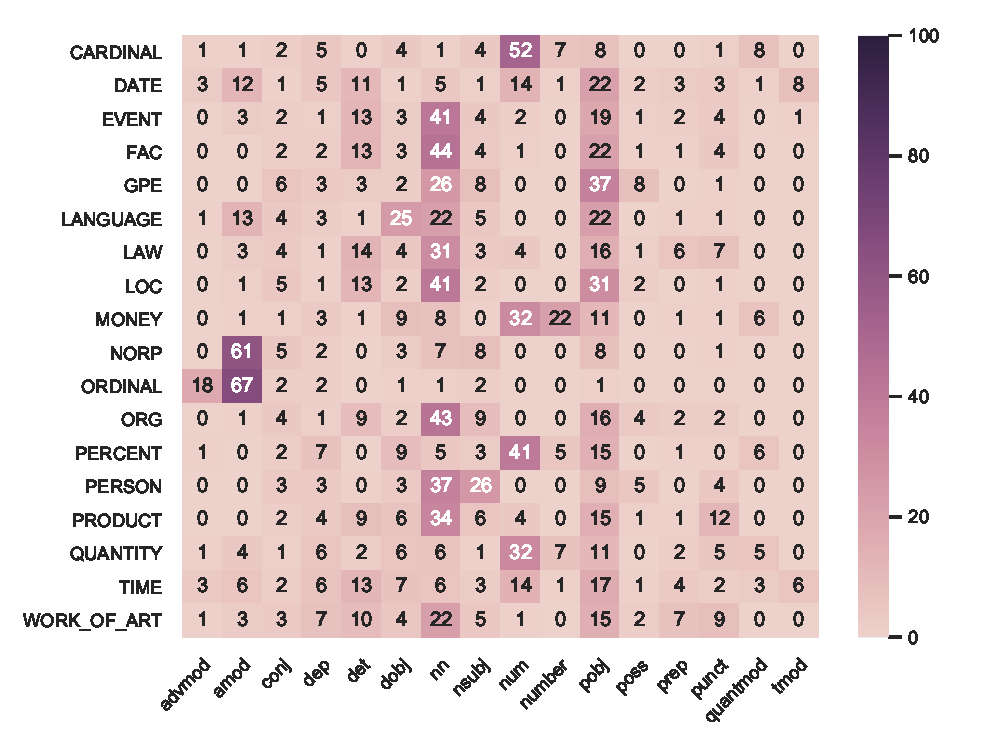
\includegraphics[width=4.8in]{Figures/depstat.eps}
	}
%	\vspace{-8mm}
	\caption{Percentage of entity words ($y$ axis) with respect to dependency relations ($x$ axis) in the OntoNotes English dataset. Columns with percentage less than 5\% are ignored for brevity.}
	%	\vspace*{-5mm}
	\label{fig:depstat}
\end{figure}

\paragraph{Baselines}
We implemented the state-of-the-art NER model \textbf{BiLSTM-CRF}~\cite{lample2016neural} as the first baseline with different number of LSTM layers ($L=\{0, 1,2,3\}$). 
$L=0$ indicates the model only relies on the input representation. 
%at most two LSTM layers ($L\leq2$). 
Following \citet{zhang2018graph}, the complete dependency trees are considered bidirectional and encoded with a contextualized GCN (BiLSTM-GCN). 
We further add the relation-specific parameters~\cite{marcheggiani2017encoding} and a CRF layer for the NER task. 
% we encode a complete dependency tree with GCN and add a CRF layer for the NER task. 
The resulting baseline is \textbf{BiLSTM-GCN-CRF}. 
We use the bootstrapping paired t-test~\cite{berg2012empirical} for significance test when comparing the results of different models.
%Details regarding the baseline models can be found in the supplementary material. 

\paragraph{BiLSTM-GCN-CRF}
Figure \ref{fig:gcnmodel} shows the neural architecture for the BiLSTM-GCN-CRF model. 
Following \citet{zhang2018graph}, the input representation at each position $\vec{w}_i$ is the word representation which consists of the pre-trained word embeddings and its character representation. 
To capture contextual information, we stack a BiLSTM layer before the GCN. 
Secondly, the GCN captures the dependency tree structure as shown in Figure \ref{fig:gcnmodel}. 
Following \citet{zhang2018graph}, we treat the dependency trees as undirected and build a symmetric adjacency matrix during the GCN update:
\begin{equation}
\vec{h}_i^{(l)}
=
\text{ReLU}
\Big(
\sum_{j=1}^{n}
A_{ij}
\mathbf{W}^{(l)} \vec{h}_j^{(l-1)}
+
\vec{b}^{(l)}
\Big)
\label{equ:gcn}
\end{equation}
where $\mathbf{A}$ is the adjacency matrix. $A_{ij} = 1$ indicates there is a dependency edge between the $i$-th word and the $j$-th word\footnote{$A_{ij} = A_{ji}$ for symmetric matrix. }. 
$\vec{h}_i^{(l)}$ is the hidden state at the $i$-th position in the $l$-th layer. 
We can stack $J$ layers of GCN in the model. 
In our experiments, we set the number of GCN layers $J = 1$ as we did not observe significant improvements by increasing $J$. 
In fact, we might obtain harmful performance for a larger $J$ as deeper GCN layers will diminish the effect of the contextual information, which is important for the task of NER. 

\begin{figure}[h!]
	\centering
	\adjustbox{max width=1\linewidth}{
		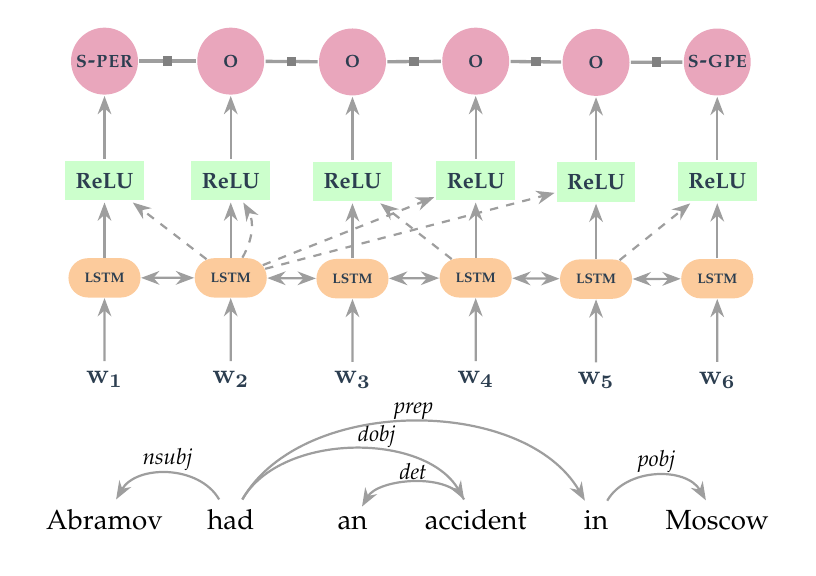
\begin{tikzpicture}[node distance=8.0mm and 10mm, >=Stealth, 
		sentity/.style={draw=none, circle, minimum height=8.5mm, minimum width=8.5mm,line width=1pt, inner sep=0pt, fill=purple!35},
		lstm/.style={draw=none, minimum height=5mm, rounded rectangle, fill=puffin!50, minimum width=11.5mm, label={center:\tiny \textcolor{fontgray}{\bf LSTM}}},
		%		, blur shadow={shadow blur steps=5}
		plus/.style={draw=none, minimum height=3mm, circle, fill={rgb:red,0;green,210;blue,211}, label={center:\footnotesize \textcolor{white}{+}}},
		gfunc/.style={draw=none, minimum height=5mm, rectangle, fill=green!20, label={center:\footnotesize \textcolor{fontgray}{\bf ReLU}}, minimum width=10mm, line width = 1.5pt},
		emb/.style={draw=none, minimum height=3mm, rounded rectangle, fill=none, minimum width=12mm, text=fontgray},
		%		cyan!40
		chainLine/.style={line width=0.8pt,->, color=mygray},
		%	background rectangle/.style={fill=olive!45}, show background rectangle, 
		%		line width=1.3pt
		]
		
		
		\matrix (s) [matrix of nodes, nodes in empty cells, execute at empty cell=\node{\strut};]
		{
			Abramov & [2ex]had & [5ex]an & [3ex]accident   &   [3ex] in  & [3ex] Moscow\\
			%		 \textbf{\textsc{date}}   &   &   & \textsc{o}     & \textsc{o}   & \textsc{o}  & \textsc{o}& \textsc{event} &  \\
		};
		
		\draw [chainLine, ->] (s-1-2) to [out=120,in=60, looseness=1] node[above, yshift=-1mm, color=black]{\footnotesize\it nsubj} (s-1-1);
		\draw [chainLine, ->] (s-1-4) to [out=120,in=60, looseness=0.8] node[above, yshift=-1mm, color=black]{\footnotesize\it det} (s-1-3);
		\draw [chainLine, ->] (s-1-2) to [out=60,in=120, looseness=0.9] node[above, yshift=-1.2mm, xshift=3mm, color=black]{\footnotesize\it dobj} (s-1-4);
		\draw [chainLine, ->] (s-1-2) to [out=60,in=120, looseness=0.9] node[above, yshift=-1mm, color=black]{\footnotesize\it prep} (s-1-5);
		\draw [chainLine, ->] (s-1-5) to [out=60,in=120, looseness=1] node[above, yshift=-1mm, color=black]{\footnotesize\it pobj} (s-1-6);
		
		\node[emb, above= of s-1-1, yshift=5mm] (u1) {$\vec{w}_\mathbf{1}$};
		\node[emb, above= of s-1-2, yshift=5mm] (u2) {$\vec{w}_\mathbf{2}$};
		\node[emb, above= of s-1-3, yshift=5.8mm] (u3) {$\vec{w}_\mathbf{3}$};
		\node[emb, above= of s-1-4, yshift=5mm] (u4) {$\vec{w}_\mathbf{4}$};
		\node[emb, above= of s-1-5, yshift=5mm] (u5) {$\vec{w}_\mathbf{5}$};
		\node[emb, above= of s-1-6, yshift=5mm] (u6) {$\vec{w}_\mathbf{6}$};
		
		\node[lstm, above= of u1] (h1) {};
		\node[lstm, above=of u2](h2) {};
		\node[lstm, above= of u3](h3) {};
		\node[lstm, above= of u4](h4) {};
		\node[lstm, above= of u5](h5) {};
		\node[lstm, above= of u6](h6) {};
		
		
		
		\node[gfunc, above= of h1, yshift=-1mm] (g1) {};
		\node[gfunc, above=of h2, yshift=-1mm](g2) {};
		\node[gfunc, above= of h3, yshift=-1mm](g3) {};
		\node[gfunc, above= of h4, yshift=-1mm](g4) {};
		\node[gfunc, above= of h5, yshift=-1mm](g5) {};
		\node[gfunc, above= of h6, yshift=-1mm](g6) {};
		
		%		\node[lstm, above= of g1, yshift=-3mm] (m1) {};
		%		\node[lstm, above=of g2, yshift=-3mm](m2) {};
		%		\node[lstm, above= of g3, yshift=-3mm](m3) {};
		%		\node[lstm, above= of g4, yshift=-3mm](m4) {};
		%		\node[lstm, above= of g5, yshift=-3mm](m5) {};
		%		\node[lstm, above= of g6, yshift=-3mm](m6) {};
		
		%		\node[left = of m1, xshift](layer1) {$L=1$};
		
		\node[sentity, above= of g1] (e1) {\footnotesize \textcolor{fontgray}{\bf \textsc{s-per}}};
		\node[sentity, above=of g2](e2) {\footnotesize \textcolor{fontgray}{\bf \textsc{o}}};
		\node[sentity, above= of g3](e3) {\footnotesize \textcolor{fontgray}{\bf \textsc{o}}};
		\node[sentity, above= of g4](e4) {\footnotesize \textcolor{fontgray}{\bf \textsc{o}}};
		\node[sentity, above= of g5](e5) {\footnotesize \textcolor{fontgray}{\bf \textsc{o}}};
		\node[sentity, above= of g6](e6) {\footnotesize \textcolor{fontgray}{\bf \textsc{s-gpe}}};
		
		
		\draw [chainLine] (u1) to (h1);
		\draw [chainLine] (u2) to (h2);
		\draw [chainLine] (u3) to (h3);
		\draw [chainLine] (u4) to (h4);
		\draw [chainLine] (u5) to (h5);
		\draw [chainLine] (u6) to (h6);
		
		\draw [chainLine] (h1) to  (g1);
		\draw [chainLine] (h2) to (g2);
		\draw [chainLine] (h3) to (g3);
		\draw [chainLine] (h4) to (g4);
		\draw [chainLine] (h5) to (g5);
		\draw [chainLine] (h6) to (g6);
		
		%		\draw [chainLine] (g1) to (m1);
		%		\draw [chainLine] (g2) to (m2);
		%		\draw [chainLine] (g3) to (m3);
		%		\draw [chainLine] (g4) to (m4);
		%		\draw [chainLine] (g5) to (m5);
		%		\draw [chainLine] (g6) to (m6);
		
		\draw [chainLine] (g1) to  (e1);
		\draw [chainLine] (g2) to   (e2);
		\draw [chainLine] (g3) to   (e3);
		\draw [chainLine] (g4) to    (e4);
		\draw [chainLine] (g5) to   (e5);
		\draw [chainLine] (g6) to   (e6);
		
		\draw [chainLine, dashed] (h2) to  [out=60,in=-60] (g2);
		\draw [chainLine, dashed] (h2) to (g1);
		\draw [chainLine, dashed] (h2) to (g4);
		\draw [chainLine, dashed] (h2) to (g5);
		\draw [chainLine, dashed] (h4) to (g3);
		\draw [chainLine, dashed] (h5) to (g6);
		
		\draw [chainLine, <->] (h1) to (h2);
		\draw [chainLine, <->] (h2) to (h3);
		\draw [chainLine, <->] (h3) to (h4);
		\draw [chainLine, <->] (h4) to (h5);
		\draw [chainLine, <->] (h5) to (h6);
		
		%		\draw [chainLine, <->] (m1) to (m2);
		%		\draw [chainLine, <->] (m2) to (m3);
		%		\draw [chainLine, <->] (m3) to (m4);
		%		\draw [chainLine, <->] (m4) to (m5);
		%		\draw [chainLine, <->] (m5) to (m6);
		
		\draw [chainLine, line width=1.2pt, -, middlefactor] (e1) to (e2);
		\draw [chainLine, line width=1.2pt, -, middlefactor] (e2)to (e3);
		\draw [chainLine, line width=1.2pt, -, middlefactor] (e3)to (e4);
		\draw [chainLine, line width=1.2pt, -, middlefactor]  (e4)to (e5);
		\draw [chainLine, line width=1.2pt, -, middlefactor] (e5)to (e6);
		
		\end{tikzpicture} 
	}
	%	\vspace*{-8mm}
	\caption{BiLSTM-GCN-CRF. Dashed connections mimic the dependency edges.}
	%	\vspace*{-5mm}
	\label{fig:gcnmodel}
\end{figure}


However, Equation \ref{equ:gcn} does not include the dependency relation information. 
We modify the Equation \ref{equ:gcn} and include the dependency relation parameter\footnote{The bias vector is ignore for brevity.}:
\begin{equation*}
\vec{h}_i^{(l)} \!= \sigma \Big(
\! \sum_{j=1}^{n}  \!
A_{ij}
\big ( 
\mathbf{W}_1^{(l)} \vec{h}_j^{(l-1)}
+ \mathbf{W}_2^{(l)}\vec{h}_j^{(l-1) }w_{r_{ij}}
\big )
%+
%\vec{b}^{(l)}
\Big)\nonumber
\end{equation*}
where $w_{r_{ij}}$ is the dependency relation weight that parameterize the dependency relation $r$ between the $i$-th word and the $j$-th word. 
Such formulation uses the relation to weight the adjacent hidden states in the dependencies. 

\paragraph{Experimental Setup}
%We implemented the state-of-the-art NER model BiLSTM-CRF as baseline~\cite{lample2016neural} with at most two LSTM layers. 
%The number of LSTM layers $L$ in DGLSTM-CRF is set to 2 and the number of GCN layers $J$ in DGGCN-CRF is set to 1. 
We choose MLP as the interaction function in our DGLSTM-CRF according to performance on the development set. 
The hidden size of all models (i.e., LSTM, GCN) is set to 200. 
We use the Glove~\cite{pennington2014glove} 100-d word embeddings, which was shown to be effective in English NER task~\cite{ma2016end,peters2018deep}. 
We use the publicly available FastText~\cite{grave2018learning} word embeddings for Chinese, Catalan and Spanish. 
%For Chinese, Catalan and Spanish, we use the FastText~\cite{grave2018learning} embeddings which are trained on Common Crawl and Wikipedia using CBOW. 
%as they provide \textcolor{red}{here}. 
%for English and FastText~\cite{grave2018learning} embeddings for the other languages.
%We use Glove~\cite{pennington2014glove} word embeddings for English and FastText~\cite{grave2018learning} embeddings for the other languages.
The ELMo~\cite{peters2018deep}, deep contextualized word representations\footnote{We also tried BERT~\cite{devlin2019bert} in preliminary experiments and obtained similar performance as ELMo. The NER performance using BERT without fine-tuning reported in \citet{peters2019tune} is consistent with the one reported by ELMo~\cite{peters2018deep}.} are used for all languages in our experiments since \citet{che2018towards} provides ELMo for many other languages\footnote{https://github.com/HIT-SCIR/ELMoForManyLangs}, including Chinese, Catalan and Spanish. 
We use the average weights over all layers of the ELMo representations and concatenate them with the input representation $\vec{u}$. 
Our models are optimized by mini-batch stochastic gradient descent (SGD) with learning rate 0.01 and batch size 10.
The $L_2$ regularization parameter is 1e-8. 
The hyperparameters are selected according to the performance on the OntoNotes English development set. 

We implemented all the models with PyTorch~\cite{paszke2017automatic}.
For both BiLSTM-CRF and DGLSTM-CRF model, we train them on all datasets with 100 epochs and take the model that perform the best on the development set. 
For BiLSTM-GCN-CRF, we train for 300 epochs with a clipping rate of 3.


\subsection{Main Results}



\paragraph{OntoNotes English}
Table \ref{tab:mainresults} shows the performance comparison between our work and previous work on the OntoNotes English dataset. 
Without the LSTM layers (i.e., $L=0$), the proposed model with dependency information significantly improves the NER performance with more than 2 points in F$_1$ compared to the baseline BiLSTM-CRF ($L=0$), which demonstrate the effectiveness of dependencies for the NER task.
Our best performing BiLSTM-CRF baseline (with Glove) achieves a F$_1$ score of 87.78 which is better than or on par with previous works~\cite{chiu2016named,li2017leveraging,ghaddar2018robust} with extra features. 
This baseline also outperforms the CNN-based models~\cite{strubell2017fast,li2017leveraging}. 
The BiLSTM-GCN-CRF model outperforms the BiLSTM-CRF model but achieves inferior performance compared to the proposed DGLSTM-CRF model. 
We believe it is challenging to preserve the surrounding context information with stacking GCN layers while contextual information is important for NER~\cite{peters2018dissecting}.
%Because stacking GCN layers is challenging to preserve the surrounding context information, which is important for the task of NER~\cite{peters2018dissecting}.
%Although BiLSTM-GCN-CRF also encoded the complete dependency trees, the last GCN layer is lack of the ability to capture the surrounding context information, which is important for the task of NER~\cite{peters2018dissecting}. 
Overall, the 2-layer DGLSTM-CRF model significantly (with $p < 0.01$) outperforms the best BiLSTM-CRF baseline and the BiLSTM-GCN-CRF model. 
As we can see from the table, increasing the number of layers (e.g., $L$ = $3$) does not give us further improvements for both BiLSTM-CRF and DGLSTM-CRF because such third-order information (e.g., the relationship among a word’s parent, its grandparent, and great-grandparent) does not play an important role in indicating the presence of named entities.
% the performance for all the models. 
%The inferior performance of BiLSTM-GCN-CRF compared to DGLSTM-CRF attribute
%A better performance for 2-layer DGLSTM-CRF compared to one layer only implies the effectiveness of the grandchild dependencies (e.g., ``(\textit{prep, pobj})''). 

\begin{table}[h!]
	\centering
%	\resizebox{\linewidth}{!}{
		\begin{tabular}{lccc}
			\toprule
			\textbf{Model}& \textbf{Prec.} & \textbf{Rec.} & \textbf{F}$_\mathbf{1}$ \\
			\midrule
			
			%			\multicolumn{3}{l}{\textbf{Pretrained Word Embedding}} &\\[1mm]
			\citet{chiu2016named}  &86.04 & 86.53 & 86.28\\
			\citet{li2017leveraging}   & 88.00 & 86.50 & 87.21 \\
			\citet{ghaddar2018robust} &- &- & 87.95 \\
			\citet{strubell2017fast} &-& -&   86.84 \\
			\cdashlinelr{1-4}
			BiLSTM-CRF ($L=0$) &82.03 & 80.78&81.40  \\
			BiLSTM-CRF ($L=1$) & 87.21 & 86.93 & 87.07 \\
			BiLSTM-CRF ($L=2$)  & 87.89 & 87.68 & 87.78 \\
			BiLSTM-CRF ($L=3$)  &  87.81& 87.50 & 87.65 \\
			%			DGGCN-CRF ($J=1$)  & 87.56 & 87.82 & 87.69 \\
			BiLSTM-GCN-CRF  &88.30 & 88.06 & 88.18 \\
			\cdashlinelr{1-4}
			DGLSTM-CRF ($L=0$) &85.31  & 82.19 & 84.09 \\
			DGLSTM-CRF ($L=1$) & \textbf{88.78} & 87.29 & 88.03 \\
			DGLSTM-CRF ($L=2$)& 88.53 & \textbf{88.50} & {\bf 88.52} \\
			DGLSTM-CRF ($L=3$)& 87.59 & 88.93 & 88.25 \\[1mm]
			
			\multicolumn{3}{l}{\textbf{Contextualized Word Representation}} &\\
			\citet{akbik2018coling} (Flair) & - & - & 89.30 \\
			\cdashlinelr{1-4}
			BiLSTM-CRF ($L=0$) + {\footnotesize ELMo} & 85.44& 84.41 & 84.92 \\
			BiLSTM-CRF ($L=1$) + {\footnotesize ELMo} & 89.14 & 88.59 & 88.87 \\
			BiLSTM-CRF  ($L=2$) + {\footnotesize ELMo}  & 88.25 & 89.71 & 88.98 \\
			BiLSTM-CRF ($L=3$) + {\footnotesize ELMo} & 88.03 & 89.04 & 88.53 \\
			
			BiLSTM-GCN-CRF +  {\footnotesize ELMo}   & 89.40 & 89.71 & 89.55 \\
			\cdashlinelr{1-4}
			DGLSTM-CRF ($L=0$) + {\footnotesize ELMo} &86.87  &85.12  &85.99 \\
			DGLSTM-CRF ($L=1$) + {\footnotesize ELMo} & 89.40 & 89.96 & 89.68 \\
			DGLSTM-CRF ($L=2$) + {\footnotesize ELMo} & \textbf{89.59} & \textbf{90.17} & {\bf 89.88} \\
			DGLSTM-CRF ($L=3$) + {\footnotesize ELMo} & 89.43 & 90.15 & 89.79 \\
			%			DGGCN-CRF (2-layer) + ELMo  & 88.80 & 89.74 & 89.27 \\
			\bottomrule
		\end{tabular}
%	}
	%	\vspace*{-3mm}
	\caption{Performance comparison on the OntoNotes 5.0 English dataset.}
	%	\vspace*{-4mm}
	\label{tab:mainresults}
\end{table}

%To further investigate if the effect of dependency would be diminished by the contextualized word representations, we compare the performance of all models with ELMo~\cite{peters2018deep} representations (Table \ref{tab:mainresults} bottom). 
We further compare the performance of all models with ELMo~\cite{peters2018deep} representations to investigate whether the effect of dependency would be diminished by the contextualized word representations. 
With $L$ = $0$, the ELMo representations largely improve the performance of BiLSTM-CRF compared to the BiLSTM-CRF model with word embeddings only but is still 1 point below our DGLSTM-CRF model. 
The 2-layer DGLSTM-CRF model outperforms the best BilSTM-CRF baseline with 0.9 points in F$_1$ ($p<0.001$).
%The improvements apply to both precision and recall. 
%We attribute the precision gain to the long-distance dependency edges and the recall gain to the dependency label information. 
Empirically, we found that among the entities that are correctly predicted by DGLSTM-CRF but wrongly predicted by BiLSTM-CRF, 47\% of them are with length more than 2. 
Our finding shows the 2-layer DGLSTM-CRF model is able to accurately recognize long entities, which can lead to a higher precision.  
%These entities have either a length more than 4 or a dependency parent far from them. 
In addition, 51.9\% of the entities that are correctly retrieved by DGLSTM-CRF have the dependency relations ``\textit{pobj}'', ``\textit{nn}'' and ``\textit{nsubj}'', which have strong correlations with certain named entity types (Figure \ref{fig:depstat}).  
Such a result demonstrates the effectiveness of dependency relations in improving the recall of NER.
%The improvements on recall also demonstrate the effectiveness of dependency relations in retrieving more entities. 





\begin{table}[h!]
	\centering
%	\resizebox{\linewidth}{!}{
		\begin{tabular}{lccc}
			\toprule
			\textbf{Model}& \textbf{Prec.} & \textbf{Rec.} & \textbf{F}$_\mathbf{1}$ \\
			\midrule
			\citet{pradhan2013towards}  &78.20 & 66.45 & 71.85\\ 
			%			\citet{nosirova2019effective}$\dagger$ & -& -& 72.40\\
			Lattice LSTM (\textcolor{darkblue}{Z\&Y, 2018}) & 76.34& 77.01& 76.67 \\
			\cdashlinelr{1-4}
			BiLSTM-CRF ($L=0$) & 76.67& 67.79& 71.95  \\
			BiLSTM-CRF ($L=1$)  & \textbf{78.45} & 74.59 & 76.47 \\
			BiLSTM-CRF ($L=2$)  & 77.94 & 75.33 & 76.61 \\
			BiLSTM-CRF ($L=3$)  & 76.17 & 75.23 & 75.70 \\
			
			BiLSTM-GCN-CRF  & 76.35 & 75.89 & 76.12 \\
			\cdashlinelr{1-4}
			DGLSTM-CRF ($L=0$) & 76.91&70.65& 73.65 \\
			DGLSTM-CRF ($L=1$)   & 77.79 & 75.29 & 76.52 \\
			DGLSTM-CRF ($L=2$)   & 77.40 & \textbf{77.41} & \textbf{77.40} \\
			DGLSTM-CRF ($L=3$)&77.01  &74.90  &75.94 \\[1mm]
			%			BiLS ($L=1$) & 77.59 & 73.67 & 75.58 \\
			\multicolumn{3}{l}{\textbf{Contextualized Word Representation}} &\\
			BiLSTM-CRF ($L=0$) + {\footnotesize ELMo} & 75.20 & 73.39 & 74.28 \\
			BiLSTM-CRF ($L=1$) + {\footnotesize ELMo}  & \textbf{79.20} & 79.21 & 79.20 \\
			BiLSTM-CRF($L=2$) + {\footnotesize ELMo}  & 78.49 & 79.44 & 78.96 \\
			BiLSTM-CRF ($L=3$) + {\footnotesize ELMo} &78.54  &79.76  &79.14 \\
			
			BiLSTM-GCN-CRF + {\footnotesize ELMo}   & 78.71 & 79.29 & 79.00 \\
			\cdashlinelr{1-4}
			DGLSTM-CRF ($L=0$) + {\footnotesize ELMo} & 76.27 & 74.61 &75.43 \\
			DGLSTM-CRF ($L=1$) + {\footnotesize ELMo}   &78.91&80.22& 79.56\\
			DGLSTM-CRF ($L=2$) + {\footnotesize ELMo}   & 78.86 & \textbf{81.00} & {\bf 79.92} \\
			DGLSTM-CRF ($L=3$) + {\footnotesize ELMo} & 79.30 &79.86  &79.58  \\
			\bottomrule
		\end{tabular}
%	}
	%	\vspace*{-2.5mm}
	\caption{Performance comparison on the OntoNotes 5.0 Chinese Dataset.}
	%	\vspace*{-4mm}
	\label{tab:mainresults_chinese}
\end{table}



\paragraph{OntoNotes Chinese}
Table \ref{tab:mainresults_chinese} shows the performance comparison on the Chinese datasets. 
\begin{table*}[h!]
	\centering
	%	\resizebox{0.8}{!}{
	\scalebox{1.0}{
		\begin{tabular}{lcccccc}
			\toprule
			\multirow{2}{*}{\textbf{Model}}&  \multicolumn{3}{c}{\textbf{Catalan}}& \multicolumn{3}{c}{\textbf{Spanish}}\\[-1mm]
			\cmidrule(lr){2-4} \cmidrule(lr){5-7} 
			& \textbf{Prec.} & \textbf{Rec.} & \textbf{F}$_\mathbf{1}$& \textbf{Prec.} & \textbf{Rec.} & \textbf{F}$_\mathbf{1}$ \\
			\midrule
			%			\multicolumn{9}{l}{\textbf{Pretrained Word Embedding}} &\\[1mm]
			BiLSTM-CRF ($L=0$) & 65.91 & 49.90 & 56.80 & 65.97&52.63&58.55  \\
			BiLSTM-CRF ($L=1$) & 76.83 & 63.47 & 69.51& 78.33 & 69.89 & 73.87 \\
			BiLSTM-CRF ($L=2$)  & 73.79 & 67.63 & 70.58 & 77.73 & 70.91 & 74.16 \\
			BiLSTM-CRF ($L=3$) & 74.75 & 67.35 & 70.86 & 76.41& 72.95 & 74.64 \\
			%			DGGCN-CRF ($L=1$) &83.38 & 84.63 & 84.00& 79.55 & 72.71 & 75.95 & 	84.82 & 78.53 & 81.55 \\
			BiLSTM-GCN-CRF    & 81.25 & 75.22 & 78.12&84.10 & 79.88 & 81.93\\
			\cdashlinelr{1-7}
			DGLSTM-CRF ($L=0$) & 73.42 & 	61.79 & 67.10& 74.90& 61.21 & 67.38\\ 
			DGLSTM-CRF ($L=1$)   & 81.87 & 79.28 & 80.55 & 83.21 & 81.19 & 82.19 \\
			DGLSTM-CRF ($L=2$)   & \textbf{83.35} & \textbf{80.00} & \textbf{81.64} & 84.05 & 82.90 &83.47\\
			DGLSTM-CRF ($L=3$) & 81.87 & 80.21 & 81.03 & \textbf{84.12} & \textbf{83.45} & \textbf{83.78}\\ 
			\multicolumn{6}{l}{\textbf{Contextualized Word Representation}} &\\[1mm]
			BiLSTM-CRF ($L=0$)  + {\footnotesize ELMo} & 67.53 & 64.47 & 65.96& 73.16 & 69.01 & 71.03\\
			BiLSTM-CRF ($L=1$) + {\footnotesize ELMo}   &77.85 & 76.22 & 77.03& 81.72 & 79.09 & 80.38 \\
			BiLSTM-CRF($L=2$) + {\footnotesize ELMo}  & 78.61 & 78.32 & 78.46 & 80.89 & 80.30 & 80.59\\
			BiLSTM-CRF($L=3$) + {\footnotesize ELMo}  & 79.11 & 77.32 & 78.21 & 80.48 & 79.45 & 79.96\\
			BiLSTM-GCN-CRF  + {\footnotesize ELMo}    &83.68 & 83.16 & 83.42 & 85.31 & 85.19 & 85.25\\
			%			DGGCN-CRF ($L=2$) + {\footnotesize ELMo}   & 83.92 & 84.86 & 84.38 & 83.61 & 83.44 & 83.52 &85.15 & 85.46 & 85.30\\
			\cdashlinelr{1-7}
			DGLSTM-CRF ($L=0$) + {\footnotesize ELMo}   & 70.87 & 65.81 & 68.25 &  75.96& 72.52 & 74.20\\
			DGLSTM-CRF ($L=1$) + {\footnotesize ELMo}    & 82.29 & 82.37 & 82.33 & 84.05 & 84.77 & 84.41\\
			DGLSTM-CRF ($L=2$) + {\footnotesize ELMo}    & \textbf{84.71} & 83.75 & \textbf{84.22}& \textbf{87.79} & \textbf{87.33} & \textbf{87.56} \\
			DGLSTM-CRF ($L=3$)  + {\footnotesize ELMo}& 84.50 & \textbf{83.92} & \textbf{84.21} & 86.74 & 86.57 & 86.66 \\
			\bottomrule
		\end{tabular}
	}
	%	\vspace*{-2.5mm}
	\caption{Results on the SemEval-2010 Task 1 datasets.}
	%	\vspace*{-3mm}
	\label{tab:semevalresult}
\end{table*}
We compare our models against the state-of-the-art NER model on this dataset, Lattice LSTM~\cite{zhang2018chinese}\footnote{We run their code on the OntoNotes 5.0 Chinese dataset.}. 
Our implementation of the strong BiLSTM-CRF baseline achieves comparable performance against the Lattice LSTM. 
Similar to the English dataset, our model with $L$ = $0$ significantly improves the performance compared to the BiLSTM-CRF ($L$ = $0$) model. 
Our DGLSTM-CRF model achieves the best performance with $L$ = $2$ and is consistently better ($p<0.02$) than the strong BiLSTM-CRF baselines. 
%Although the 2-layer DGLSTM-CRF model consistently achieves the best results in F$_1$ ($p<0.05$) compared to our strong BiLSTM-CRF baselines, the improvements are not as significant as in the English dataset. 
%The DGGCN-CRF obtains only comparable performance against the baselines. 
As we can see from the table, the improvements of the DGLSTM-CRF model mainly come from recall ($p<0.001$) compared to the BiLSTM model, especially in the scenario with word embeddings only. 
%Such improvements leverage the ability of dependency relations in helping to predict more entities. 
Empirically, we also found that those correctly retrieved entities of the DGLSTM-CRF (compared against the baseline) mostly correlate with the following dependency relations: ``\textit{nn}'', ``\textit{nsubj}'', ``\textit{nummod}''.
However, DGLSTM-CRF achieves lower precisions against BiLSTM-CRF, which indicates that the DGLSTM-CRF model makes more false-positive predictions. 
%The reason could be that there are some dependency relations that strongly correlates entity words also correlate to non-entity words. 
%As such, the model would tend to predict the words  with those dependency relations  as entities while these words are actually non-entity. 
The reason could be the relatively lower ratio of ST(\%)\footnote{Percentage of entities that can form a subtree.} as shown in Table \ref{tab:datastat}, which means some of the entities do not form subtrees under the complete dependency trees. 
In such a scenario, the model may not correctly identify the boundary of the entities, which results in lower precision. 
%We found that the number of correctly predicted entities by DGLSTM-CRF is actually larger than the one by BiLSTM-CRF. 
%However, the DGLSTM-CRF predicted more entities and achieved lower precision, which might be caused by some dependency labels that intend to predict more entities. 

%The contextualized word representation is able to significantly improve the recall 
%Only recall improved. Chinese low agreement rate 
%low parsing performance. lower than English








\paragraph{SemEval-2010} 

%Table \ref{tab:semevalresult} shows the results of our models on the SemEval-2010 Task 1 datasets. 
%%The results marked in bold are significantly better than the best performing BiLSTM-CRF baseline. 
%As the English dataset is a subset of the OntoNotes English corpus, we obtain similar performance as in the OntoNotes 5.0 English dataset where the DGLSTM-CRF achieves the best performance ($p<0.05$) in precision, recall and F$_1$. 
%The improvement are not as significant as in the OntoNotes English dataset. 
%The reason is similar to the Chinese dataset where we have a relatively low ST(\%) in this dataset. 

Table \ref{tab:semevalresult} shows the results of our models on the SemEval-2010 Task 1 datasets.
Overall, we observe substantial improvements of the DGLSTM-CRF on the Catalan and Spanish datasets (with $p<0.001$ marked in bold against the best performing BiLSTM-CRF baseline), especially for DGLSTM-CRF with ELMo and $L$ larger than 1.  
%Such improvements demonstrate the effectiveness of the DGLSTM-CRF in encoding the dependency trees for NER. 
With word embeddings, the best DGLSTM-CRF model outperforms the best performing BiLSTM-CRF baseline with more than 10 and 9 points in  F$_1$  on the Catalan and Spanish datasets, respectively. 
The BiLSTM-GCN-CRF model also performs much better than the BiLSTM-CRF baselines but is worse than the DGLSTM-CRF model with $L\geq 2$. 
%The improvements over the BiLSTM-GCN-CRF further shows the importance of 
%the DGLSTM-CRF model has more than 10\% F$_1$ improvement over the BiLSTM-CRF model on the Catalan dataset and about 9\% improvement on the Spanish dataset. 
Both precision and recall significantly improve with a large margin compared to the best performing BiLSTM-CRF, especially for the recall (with more than 10 points improvement) on these two datasets. 
With ELMo, the best performing DGLSTM-CRF model outperforms the BiLSTM-CRF baseline with about 6 and 7 points in F$_1$ on these two datasets, respectively. 
The substantial improvements show that the structural dependency information is extremely helpful for these two datasets. 
%the performance of BiLSTM-CRF improves for more than 6 points in  F$_1$. 
%On the other hand, the F$_1$ of the DGLSTM-CRF with 1 layer also increases for these two languages and still significantly better than the baselines.

%Such improvements not only apply to recall but precision as well. 
%The absolute improvements is even larger than the one we observe in the OntoNotes English datasets. 

%The improvement of DGGCN-CRF is not as significant as DGLSTM-CRF, showing that the DGLSTM-CRF is more robust across different languages and the ability of LSTM that captures the contextualized information is important for the NER task. 

With ELMo representations, we observe about 2 and 3 points improvements in F$_1$  compared with the 1-layer DGLSTM-CRF model on these two datasets, respectively. 
%We further compare the results between the 1-layer DGLSTM-CRF and 2-layer DGLSTM-CRF (with ELMo) models to investigate their differences in the Catalan and Spanish datasets. 
%Empirically, the 2-layer DGLSTM-CRF model improves the the performance of all entity types (e.g., \textsc{person}) compared to the 1-layer DGLSTM-CRF model. 
Empirically, more than 50\% of the entities that are correctly predicted by the 2-layer model but not the 1-layer model are with length larger than 2.
%Empirically, the performance of all entity types (e.g., \textsc{person}) is improved by 
%has significant improvement with the 2-layer model. 
%Among the entities that are correctly recognized by 2-layer model but not 1-layer model, more than 50\% of them are entities with length more than 2. 
%We found that, among the entities correctly predicted  by the 2-layer model but not the 1-layer , more than 50\% of them with length larger than 2. 
Also, most of these entities contain the grandchild dependencies ``(\textit{sn, sn})'' and ``(\textit{spec, sn})'' where \textit{sn} represents noun phrase and \textit{spec} represents specifier (e.g., determiner, quantifier) in both datasets. 
Such a finding shows that the 2-layer model is able to capture the interactions given by the grandchild dependencies. 
%The substantial improvements show that the 2-layer DGLSTM-CRF is able to reasoning over the dependency edges and such reasoning immediately benefits the named entity recognition. 
%Following the dependency structures and stacking the LSTM enable the model learn from these evidences. 
%





%\paragraph{Limited Training Data}
%
%\begin{figure}[h]
%	\centering
%	\resizebox{0.7\linewidth}{!}{
%	\begin{tikzpicture}[]
%	\begin{axis}[
%	xlabel=\% of Training Data,
%	ylabel=$F_1$,
%	y label style={at={(axis description cs:0.05,.5)}},
%	legend pos=south east,
%	legend style={font=\tiny}
%	]
%	
%	\addplot[smooth,mark=*,myblue!90, line width=1pt] plot coordinates {
%		(10,84.05)
%		(20,86.45)
%		(30,87.02)
%		(40,87.77)
%		(50,87.88)
%		(60,88.17)
%		(70,88.55)
%		(80,88.56)
%		(90,88.60)
%		(100,88.87)
%	};
%	\addlegendentry{LSTM-CRF}
%	
%	\addplot[smooth,color=myred!90,mark=square*, line width=1pt]
%	plot coordinates {
%		(10,85.27)
%		(20,87.52)
%		(30,88.22)
%		(40,88.88)
%		(50,88.86)
%		(60,89.23)
%		(70,89.28)
%		(80,89.49)
%		(90,89.62)
%		(100,89.97)
%	};
%	\addlegendentry{DGLSTM-CRF}
%	
%	\addplot[smooth,color=puffin!90,mark=triangle*, line width=1pt]
%	plot coordinates {
%%		(10,85.27)
%%		(20,87.52)
%%		(30,88.22)
%%		(40,88.88)
%%		(50,88.86)
%%		(60,89.23)
%%		(70,89.28)
%%		(80,89.49)
%%		(90,89.62)
%		(100,89.70)
%	};
%	\addlegendentry{DGGCN-CRF}
%	\end{axis}
%	\end{tikzpicture}
%	}
%	\caption{Performance on OntoNotes English against the percentage of training data.}
%	\label{res:ontonoteslimited}
%\end{figure}
%


%\begin{table}[t!]
%	\centering
%	\setlength{\tabcolsep}{4pt} % Default value: 6pt
%	\renewcommand{\arraystretch}{1.0} % Default value: 1
%	\resizebox{0.9\linewidth}{!}{
%	\begin{tabular}{lcccccc}
%		\toprule
%		\multirow{2}{*}{Model} & \multicolumn{3}{c}{\textbf{Afrikaans}}& \multicolumn{3}{c}{\textbf{Swedish}}\\
%		 & \textbf{Prec.} & \textbf{Rec.} & \textbf{F}$_\mathbf{1}$ & \textbf{Prec.} & \textbf{Rec.} & \textbf{F}$_\mathbf{1}$ \\
%		\midrule
%		BiLSTM-CRF & 70.63& 51.76&59.74 & 64.58 & 19.80 & 30.00\\
%		DGLSTM-CRF & 71.70&54.23 &61.75 & 69.21 & 27.84 & 39.71\\
%		\bottomrule
%	\end{tabular}
%	}
%	\caption{Results for low-resource NER.}
%	\label{tab:lowresource}
%\end{table}
%
%\subsection{Low-Resource Named Entity Recognition}
%To further evaluate the robustness of the dependency structures, we conduct experiments under a low-resource setting. 
%We use two open-source NER corpora\footnote{https://github.com/juand-r/entity-recognition-datasets} in Afrikaans and Indonesian. 
%Following \citet{cotterell2017low}, we only use 100 sentences in training to emulate the truly low-resource situation. 
%We use FastText word embeddings and the latest Stanford Dependency parser~\cite{qi2018universal} to obtain the dependency trees. 
%Table \ref{tab:lowresource} shows the results of the baseline and DGLSTM-CRF model with 1 LSTM layer. 
%With limited amount of training data, the LSTM-CRF models including feature-based CRF~\cite{lafferty2001conditional} suffer from low recall as it is difficult to generalize to unseen data and easily to overfit the training data. 
%The DGLSTM-CRF significantly improves the recall, showing the robustness of the dependency in retrieving more entities. 
%%Due to limited amount of data and quality of dependencies, the absolute improvement in precision is not as high as recall. 

%\begin{table}[t!]
%	\centering
%	\resizebox{1.0\linewidth}{!}{
%	\begin{tabular}{lcccccc}
%		\toprule
%		\multirow{2}{*}{Model}& \multicolumn{3}{c}{\textbf{Development}} & \multicolumn{3}{c}{\textbf{Test}}\\
%		&  \textbf{Prec.} & \textbf{Rec.} & \textbf{F}$_\mathbf{1}$ &  \textbf{Prec.} & \textbf{Rec.} & \textbf{F}$_\mathbf{1}$ \\
%		\midrule
%		DGLSTM-CRF & 87.47& 88.73 & 88.10&89.43 & 90.24 & 89.83 \\
%		  ~~--$g(\cdot) = $ Concatenation & 87.30 & 88.84 & 88.06 & 89.45 & 90.18 &89.81 \\
%		  ~~--$g(\cdot) = $ Addition & 86.88& 88.41& 87.41& 89.23 & 89.90 &89.57 \\
%		  ~~--w/o dependency relation & 87.14 & 88.59 &87.86 & 88.92 & 89.99 & 89.45\\
%		  ~~--with Universal dependency & 87.33 &89.33 & 88.32 & 89.10 & 90.30 & 89.70\\
%		  ~~--with predicted dependency &87.51 &88.04 & 87.78 & 89.41 & 89.11 &89.26 \\
%		  \bottomrule
%	\end{tabular}
%}
%	\vspace{-3mm}
%	\caption{Ablation study of the DGLSTM-CRF model on OntoNotes dataset.}
%	\label{tab:ablation}
%\end{table}


%\paragraph{CoNLL-2003 English} 


\subsection{Additional Experiments}
%We conduct additional experiments on the CoNLL-2003 English dataset and ablation study on the OntoNotes English dataset. 
%
\paragraph{CoNLL-2003 English}
Table \ref{tab:resconll} shows the performance on the CoNLL-2003 English dataset. 
The dependencies are predicted from Spacy~\cite{spacy2}. 
With the contextualized word representations, DGLSTM-CRF outperforms BiLSTM-CRF with 0.2 points in F$_1$ ($p<0.09$). 
%The improvement is not significant due to the relatively low ST ratio as shown Table \ref{tab:datastat}. 
The improvement is not significant due to the relatively lower equality of the dependency trees. 
To further study the effect of the dependencies, we modified the predicted dependencies to ensure each entity form a subtree in the complete dataset. 
Such modification improves the F$_1$ to 92.7, which is significantly better ($p<0.05$) than the BiLSTM-CRF.

\begin{table}[h!]
	\centering
	%	\resizebox{1.0\linewidth}{!}{
	% 	\scalebox{0.6}{
	\begin{tabular}{lccc}
		\toprule
		%			\multirow{2}{*}{\bf Model}& \multicolumn{3}{c}{\textbf{Test}} \\
		\textbf{Model} & \textbf{Prec.} & \textbf{Rec.} &   \textbf{F}$_\mathbf{1}$\\
		\midrule
		\citet{peters2018deep}~ ELMo  &  -& - &92.2 \\
		\cdashlinelr{1-4}
		BiLSTM-CRF  + {\footnotesize ELMo ($L=2$)}  &  92.1 & 92.3 &    92.2 \\
		DGLSTM-CRF + {\footnotesize ELMo ($L=2$)} & 92.2&92.5 &92.4\\
		\bottomrule
	\end{tabular}
	%	}
	%	\vspace{-2.5mm}
	\caption{Performance on the CoNLL-2003 English dataset.}
	%	\vspace{-1.5mm}
	\label{tab:resconll}
\end{table}

%Similar to the SemEval English and OntoNotes Chinese datasets, the moderate  improvements are caused by the relatively low ST ratio as shown in Table \ref{tab:datastat}. 




\paragraph{Low-Resource NER}
Following \citet{cotterell2017low}, we emulate truly low-resource condition with 100 sentences for training.
We assume that the contextualized word representations are not available and dependencies are predicted. 
Table \ref{tab:lowresources} shows the NER performance on the SemEval-2010 Task 1 datasets under the low-resource setting. 
With limited amount of training data, BiLSTM-CRF suffers from low recall and the DGLSTM-CRF largely improves it on these two datasets. 
Using gold dependencies further significantly improves the precision and recall. 

\begin{table}[h!]
	\centering
	%	\resizebox{1.0\linewidth}{!}{
	%	\scalebox{0.8}{
	\begin{tabular}{lcccccc}
		\toprule
		\multirow{2}{*}{\textbf{Model}}&  \multicolumn{3}{c}{\textbf{Catalan}}& \multicolumn{3}{c}{\textbf{Spanish}}\\[-1mm]
		\cmidrule(lr){2-4} \cmidrule(lr){5-7} 
		& \textbf{Prec.} & \textbf{Rec.} & \textbf{F}$_\mathbf{1}$& \textbf{Prec.} & \textbf{Rec.} & \textbf{F}$_\mathbf{1}$ \\
		\midrule
		%			\multicolumn{9}{l}{\textbf{Pretrained Word Embedding}} &\\[1mm]
		BiLSTM-CRF ($L=1$) & 47.88 & 18.59 & 26.78 & 40.77 & 19.01 & 25.93 \\
		DGLSTM-CRF ($L=1$) & 47.71 & 31.55 & 37.98&  49.39 & 31.91 & 38.77\\
		~~-- with gold dependency & \textbf{52.13} & \textbf{33.26} & \textbf{40.61} & \textbf{52.14} & \textbf{35.59} & \textbf{42.30} \\
		\bottomrule
	\end{tabular}
	%	}
	%	\vspace*{-2.5mm}
	\caption{Low-resource NER performance on the SemEval-2010 Task 1 datasets.}
	%	\vspace*{-4mm}
	\label{tab:lowresources}
\end{table}
%Further gold dependency annotations can 
%We can see that the DGLSTM-CRF largely improves the recall 

% \begin{table}[t!]
%     \centering
%     \resizebox{1.0\linewidth}{!}{
%     \begin{tabular}{lcccc}
%         \toprule
%          & English & Chinese & Catalan & Spanish \\
%          \midrule
%         UAS &96.0 & 91.4& 95.2& 95.3\\
%         LAS & 94.9&89.3 &93.3 & 93.4\\
%         \bottomrule
%     \end{tabular}
%     }
%     \caption{The performance of dependency parser on all languages. UAS and LAS represent the unlabeled and labeled attachment scores, respectively.}
%     \label{tab:dep_result}
% \end{table}

% \begin{table}[t!]
% 	\centering
% 	\resizebox{1\linewidth}{!}{
% 		\begin{tabular}{lccccccc}
% 			\toprule
% 			\multirow{2}{*}{\textbf{Dataset}}&  \multicolumn{3}{c}{\textbf{Gold Dependency}}& \multicolumn{4}{c}{\textbf{Predicted Dependency}}\\[-1mm]
% 			\cmidrule(lr){2-4} \cmidrule(lr){5-8} 
% 			& \textbf{Prec.} & \textbf{Rec.} & \textbf{F}$_\mathbf{1}$ & \textbf{LAS}& \textbf{Prec.} & \textbf{Rec.} & \textbf{F}$_\mathbf{1}$ \\
% 			\midrule

% 			English & 89.59 & 90.17 & 89.88 & 94.9 & 89.62 & 89.67 & 89.64\\
% 			Chinese &  78.86 & 81.00 &79.92 & 89.3 & 78.51 & 80.70 & 79.59\\
% 			Catalan & 84.71 & 83.75 & 84.22 & 93.3 & 83.28 & 81.48 & 82.37\\
% 			Spanish &  87.79& 87.33 & 87.56 & 93.4 &  83.28 & 84.57 & 83.92\\
% 			\bottomrule
% 		\end{tabular}
% 	}
% %	\vspace*{-3mm}
% 	\caption{Performance comparision.}
% %	\vspace*{-4mm}
% 	\label{tab:dep_result}
% \end{table}






\paragraph{Effect of Dependency Quality}
% In practice, it is laborious to obtain parse tree annotations for a sentence. 
To evaluate how the quality of dependency trees affect the performance, we train a state-of-the-art dependency parser~\cite{dozat2017deep} using our training set and make prediction on the development/test set. 
We train a BERT-based~\cite{devlin2019bert} dependency parser~\cite{dozat2017deep} using the training set for each of four languages. 
Specifically, we adopt the \texttt{bert-base-uncased} model for English, \texttt{bert-base-multilingual-cased} for Catalan and Spanish and \texttt{bert-base-chinese} for Chinese.
Because the Chinese BERT model is based on characters but not Chinese words which are segmented. 
We further incorporate a span extractor layer right after BERT encoder for Chinese. 
We following \citet{lee2017end} to design the span extractor layer. Our code for dependency parser is available at \url{https://github.com/allanj/bidaf_dependency_parsing}
We implemented the dependency parser using the AllenNLP package~\cite{Gardner2017AllenNLP}.
Table \ref{tab:dep_result} shows the performance (LAS) of the dependency parser on four languages (i.e., OntoNotes English, OntoNotes Chinese, Catalan and Spanish) and the performance of DGLSTM-CRF against the best performing BiLSTM-CRF with ELMo.
% As we can see, the dependency performance on Chinese is relatively worse than the performance on other languages. 
% We attribute this performance to 
DGLSTM-CRF even with predicted dependencies is able to consistently outperform the BiLSTM-CRF on four languages. 
However, the performance is still worse than the DGLSTM-CRF with gold dependencies, especially on the Catalan and Spanish.
Such results suggest that it is essential to have high-quality dependency annotations available for the proposed model.
% However, the dependency parsers are not perfect enough to obtain completely accurate parse trees.
% Such predicted dependencies make the performance of DGLSTM-CRF worse than the DGLSTM-CRF with gold dependencies, especially on the Catalan and Spanish languages where the dependencies are more effective as shown in Table \ref{tab:semevalresult}.
% We can see the performance on Chinese is not good.

\begin{table}[h!]
	\centering
	%	\resizebox{1\linewidth}{!}{
	\begin{tabular}{lcccc}
		\toprule
		& \textbf{English} & \textbf{Chinese} & \textbf{Catalan} & \textbf{Spanish} \\
		\midrule
		BiLSTM-CRF & 88.98 & 79.20 & 78.46 & 80.59 \\
		\midrule
		(Dependency LAS)$\dagger$ & (94.89) & (89.28) & (93.25) & (93.35)\\
		DGLSTM-CRF (Predicted) & \textbf{89.64} & \textbf{79.59} & \textbf{82.37} & \textbf{83.92} \\
		Improvement $\Delta$ & +0.66 & +0.39 & +3.91 & +3.33\\
		\midrule \midrule
		DGLSTM-CRF (Gold) & 89.88 & 79.92 & 84.22 & 87.56 \\ 
		\bottomrule
	\end{tabular}
	%	}
	%	\vspace*{-3mm}
	\caption{F$_1$ performance of DGLSTM-CRF with predicted dependencies against the best performing BiLSTM-CRF. $\dagger$: LAS is label attachment score which is the metric for dependency evaluation.}
	%	\vspace*{-4mm}
	\label{tab:dep_result}
\end{table}

\paragraph{Ablation Study}
%We conduct ablation study in Table \ref{tab:ablation} on the best performing 2-layer DGLSTM-CRF model. 
Table \ref{tab:dglstmablation} shows the ablation study of the 2-layer DGLSTM-CRF model on the OntoNotes English dataset.
With self connection as interaction function, the F$_1$ drops 0.3 points.
The model achieves comparable performance with concatenation as interaction function but  F$_1$ drops about 0.4 points with the addition interaction function.  
We believe that the addition potentially leads to certain information loss.
Without the dependency relation embedding $\vec{v}_r$ in the input representation, the F$_1$ drops about 0.4 points.
%We also tried with the Universal dependency representation\footnote{https://universaldependencies.org/} converted from the Stanford CoreNLP Toolkit. 
%The performance on development set increase about 0.2\% in F$_1$ but it does not generalize to the test set. 
%The performance on development set increase about 0.2\% in F$_1$. 
% Using predicted dependency from Spacy~\cite{spacy2} degrade the performance for about 0.6 points, which shows that the quality of dependency is important for achieving high performance. 
% Overall, the performance with predicted dependencies is still better than the best performing BiLSTM-CRF. 
\begin{table}[h!]
	\centering
	%	\resizebox{1.0\linewidth}{!}{
	\begin{tabular}{lccc}
		\toprule
		%			\multirow{2}{*}{\bf Model}& \multicolumn{3}{c}{\textbf{Test}} \\
		\textbf{Model}&  \textbf{Prec.} & \textbf{Rec.} & \textbf{F}$_\mathbf{1}$\\
		\midrule
		BiLSTM-CRF + {\footnotesize ELMo ($L=2$)}  & 89.14& 88.59 & 88.87 \\
		\cdashlinelr{1-4}
		DGLSTM-CRF  + {\footnotesize ELMo ($L=2$)}  & \textbf{89.59}& \textbf{90.17} & \textbf{89.88} \\
		~~~--$g(\cdot) = $ self connection & 89.17 &90.08  &89.62   \\
		~~~--$g(\cdot) = $ Concatenation & 89.43 & 90.09 & 89.76  \\
		~~~--$g(\cdot) = $ Addition & 89.24&89.78 & 89.50\\
		~~~--w/o dependency relation & 88.92 & 89.99 & 89.46 \\
		%			~~--with Universal dependency & 87.33 &89.33 & 88.32 \\
		% 			~~~--with predicted dependency &89.62 & 89.67 & 89.64 \\
		\bottomrule
	\end{tabular}
	%	}
	%	\vspace{-2.5mm}
	\caption{Ablation study of the DGLSTM-CRF model on the OntoNotes English dataset.}
	%	\vspace{-3mm}
	\label{tab:dglstmablation}
\end{table}







%\section{Baseline Systems}
%We implemented the BiLSTM-CRF~\cite{lample2016neural} and BiLSTM-GCN-CRF models based on the contextualized GCN implementation by \citet{zhang2018graph}. 
%The implementation of BiLSTM-CRF is exactly same as \citet{lample2016neural}. 
%We presents the neural architecture for the BiLSTM-GCN-CRF model. 









\section{Analysis}
\label{sec:analysis}
% We conduct analysis with the 2-layer DGLSTM-CRF on the OntoNotes English dataset.
\subsection{Effectiveness of Dependency Relations}
To demonstrate whether the model benefits from the dependency relations, we first select the entities that are correctly predicted by the 2-layer DGLSTM-CRF model but not by the best performing baseline 2-layer BiLSTM-CRF on the OntoNotes English dataset. 
We draw the heatmap in Figure \ref{fig:deprelana} based on these entities.  
Comparing Figure \ref{fig:depstat} and \ref{fig:deprelana}, we can see that they are similar in terms of the density. 
Both of them show consistent relationships between the entity types and the dependency relations. 
The comparison shows that the improvements partially result from the effect of dependency relations. 
We also found from our model's predictions that some entity types have strong correlations with the relation pairs on grandchild dependencies. 

\begin{figure}[h!]
	\centering
	\scalebox{1.0}{
		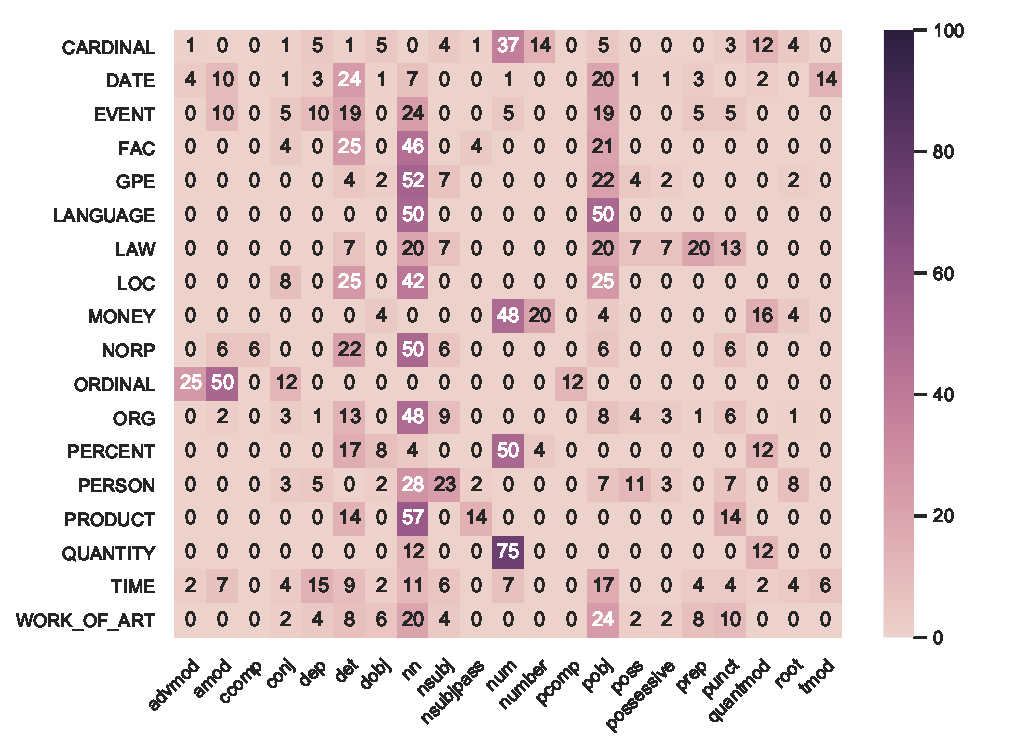
\includegraphics[width=4.5in]{Figures/deprelana.eps}
	}
	%	\vspace{-8mm}
	\caption{Correlations between the correctly predicted entities and the dependency relations.}
	\label{fig:deprelana}
	%	\vspace{-2mm}
\end{figure}

\subsection{Entity with Different Lengths}
Table \ref{tab:reslength} shows the performance comparison with different entity lengths on all datasets. 
As mentioned earlier, the dependencies as well as the grandchild relations allow our models to capture the long-distance interactions between the words. 
% The performance of NER can benefit from such long-distance interactions, especially for long entities. 
As shown in the table, the performance of entities with lengths more than 1 consistently improves with DGLSTM-CRF for all languages except Chinese.
As we pointed out in the dataset statistics (Table \ref{tab:datastat}),  the number of entities that form subtrees in OntoNotes Chinese is relatively smaller compared to other datasets.
The performance gain is more significant for entities with longer length on the other three languages. 
We found that, among the improvements of entities with length larger than 2 in English, 85\% of them have long-distance dependencies and 30\% of them have grandchild dependencies within the entity boundary. 
The analysis shows that our model that exploits the dependency tree structures is helpful for recognizing long entities.
%Such result statistics show the DGLSTM-CRF is able to capture the long-distance interactions. 
%



\begin{table}[h!]
	\centering
	%	\resizebox{1.0\linewidth}{!}{
	\begin{tabular}{clcccccc}
		\toprule
		\multirow{2}{*}{\textbf{Dataset}}& \multirow{2}{*}{\textbf{Model}} & \multicolumn{6}{c}{\textbf{Entity Length}} \\
		& & \textbf{1} & \textbf{2} & \textbf{3} & \textbf{4} & \textbf{5}  & $\mathbf{\geq}$\textbf{6}  \\
		\midrule
		\multirow{2}{*}{\textbf{English}} & BiLSTM-CRF & \textbf{91.8} & 88.5 & 83.4 & 84.0 & 75.4 & 76.0 \\
		& DGLSTM-CRF & \textbf{91.8} &  \textbf{90.1} &  \textbf{85.4}&  \textbf{87.0} &  \textbf{80.8} &  \textbf{78.7} \\ 
		\midrule
		\multirow{2}{*}{\textbf{Chinese}} & BiLSTM-CRF &81.2 & 74.3 & \textbf{73.1} & 62.8 & \textbf{70.3} & \textbf{57.5} \\
		& DGLSTM-CRF & \textbf{82.2}& \textbf{75.5} & 71.8 & \textbf{64.1} & 58.5 & 41.1\\
		\midrule
		\multirow{2}{*}{\textbf{Catalan}} & BiLSTM-CRF &80.5 & 81.0 & 75.8 & 56.1 & 45.0 & 38.4\\
		& DGLSTM-CRF & \textbf{85.4} & \textbf{85.1} & \textbf{84.1} & \textbf{78.9} & \textbf{60.9} & \textbf{59.3}\\
		\midrule
		\multirow{2}{*}{\textbf{Spanish}} & BiLSTM-CRF & 84.2 & 81.1 & 81.0 & 53.3 & 53.3 & 37.1\\
		& DGLSTM-CRF & \textbf{89.3} & \textbf{87.4} & \textbf{90.8} & \textbf{74.1} & \textbf{67.7} & \textbf{64.4}\\
		
		\bottomrule
	\end{tabular}
	%	}
	%		\vspace{-2.5mm}
	\caption{Performance of entities with different lengths on the four datasets: OntoNotes (English), OntoNotes Chinese, Catalan and Spanish.}
	%	\vspace{-3mm}
	\label{tab:reslength}
\end{table}









\section{Relation Pairs on Grandchild Dependencies}
Figure \ref{fig:gd} visualized the correlations between the entities and the grandchild dependency relation pairs on the OntoNotes English dataset. 
As we can see from the figure, most of these entities correlate to the ``(\textit{nn}, \textit{nn})'' and ``(\textit{nn}, \textit{pobj})'' relation pairs on the grandchild dependencies. 
Such correlations also show that the relation pair information on the grandchild dependencies can be helpful for detecting certain entities. 

\begin{figure*}[h!]
	\centering
	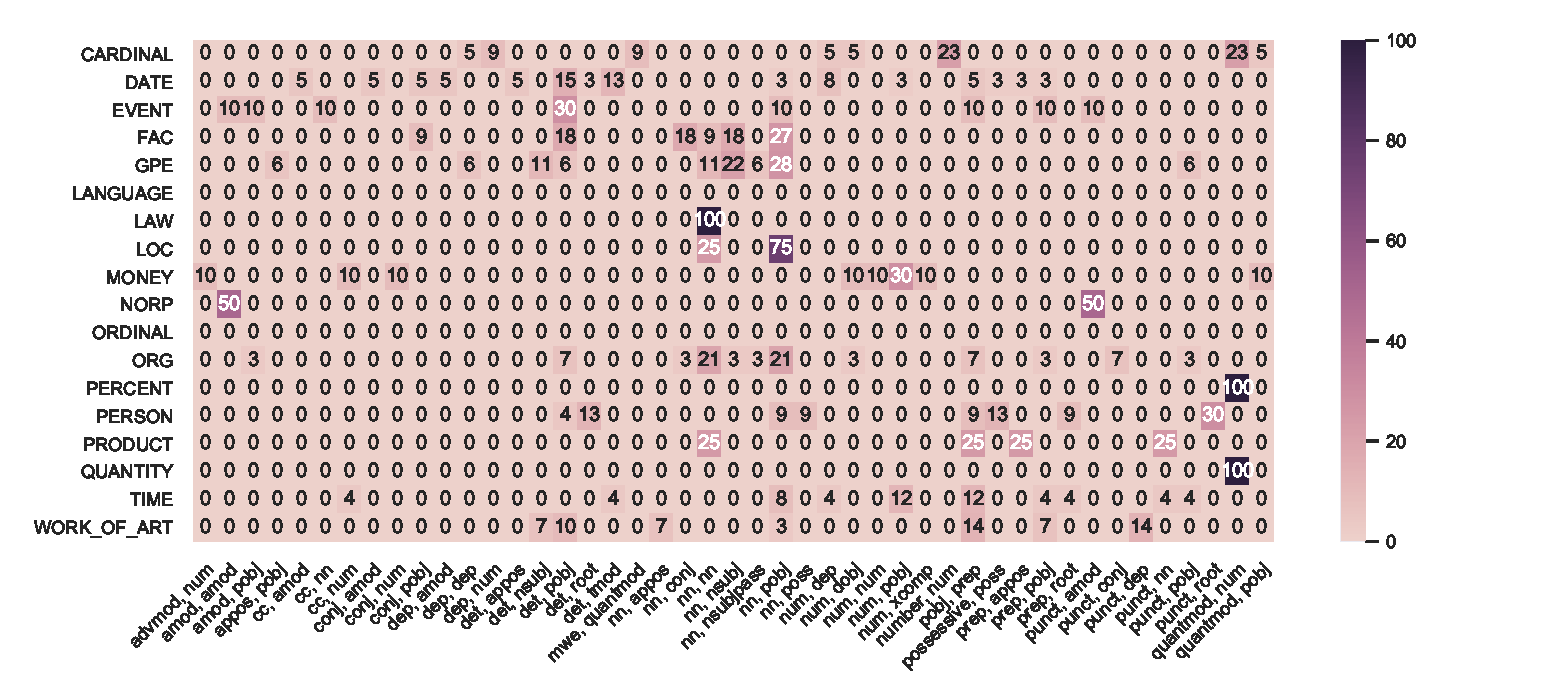
\includegraphics[width=6.2in]{Figures/gdrelana.eps}
	\caption{Correlations between the entity types and the dependency relation pairs on the grandchild dependencies.}
	\label{fig:gd}
\end{figure*}

\section{Conclusions}
Motivated by the relationships between the dependency trees and named entities, we propose a dependency-guided LSTM-CRF model to encode the complete dependency tree and capture such relationships for the NER task. 
Through extensive experiments on several datasets, we demonstrate the effectiveness of the proposed model in improving the NER performance. 
Such improvements also generalize to a low-resource setting. 
Our analysis shows that NER benefits from the dependency relations and long-distance dependencies, which are able to capture the non-local interactions between the words. 
%Our quantified analysis show that NER benefits from the dependency relations and the long-distance interactions between the words. 

As statistics shows that most of the entities form subtrees under the dependency trees, future work includes building a model for joint NER and dependency parsing which regards each entity as a single unit in a dependency tree. 


\section{Learning Latent Dependency for Named Entity Recognition (Future Work)}
Dependency tree structures have been proven to have a strong relationship with named entities~\cite{jie2019dependency}. 
The underlying properties (e.g., dependency relations correlate to entity types) are evidently helpful for the named entity recognition (NER) task.
However, creating dependency annotations for NER datasets could be expensive and laborious, especially in low-resource languages.
We discuss a possible solution where we treat the dependency trees as latent variables for named entity recognition.

\subsection{Dependency Trees as Latent Variables}
In this problem, dependency tree serves as a structured latent variable~\cite{martins2019latent} during the inference process as shown in Figure \ref{fig:latenttree}. 
Equation \ref{equ:latenttree} shows the marginalization over all the trees $\vec{h}$.
As enumerating all the possible dependency trees $\vec{h}$ is intractable, we need some approximations for tractable inference. 
\begin{equation}
P(\vec{y} \vert \vec{x}) = \sum_{ \vec{h} } P (\vec{y}, \vec{h} \vert \vec{x})
\label{equ:latenttree}
\end{equation}
For example, \citet{corro2019learning} proposed a sampling mechanism to sample dependency trees from the tree distribution. 
They apply the reparameterization trick to make the process differentiable, which in turns make the complete model differentiable. 
There are some other literature working on the same problem: making the latent variable differentiable (e.g., straight-through estimator~\cite{bengio2013estimating}).
Thus, as the intermediate step of our dependency-guided LSTM-CRF model, we aim to apply these techniques for further attempt where we do not require the dependency trees to be available.

\begin{figure*}[h!]
	\centering
	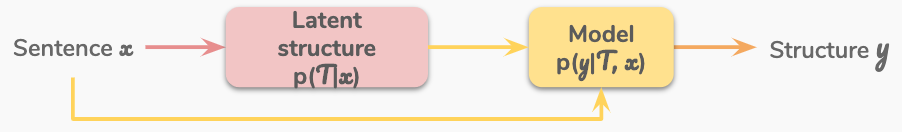
\includegraphics[width=4.2in]{Figures/latent_tree.png}
	\caption{Dependency trees as latent variables for our NER task.}
	\label{fig:latenttree}
\end{figure*}

\subsection{Multi-task Learning}
In order to further improve the performance, we are able to jointly train the dependency dataset where we can have the joint loss from dependency and named entity performance.
The nice thing is that we do not require a dataset to have both named entity and dependency annotations. 
We can train the complete module with separate dependency and named entity datasets.

\section{Connections between the DGLSTM-CRF and DGM in Chapter \ref{Chapter3}}
We discuss the connections between the DGM in Chapter \ref{Chapter3} and the DGLSTM-CRF model in this section. 
\paragraph{Dependency-Guided Model based on Semi-Markov CRF}
The dependency-guided model (DGM)~\cite{jie2017efficient} is our first proposed model, which was motivated by the evidence that entities often form subtrees in the dependency trees.
It is a model based on the semi-Markov CRF~\cite{sarawagi2004semi}. 
In short, the DGM model achieves comparable or better performance with much faster inference speed compared with the semi-Markov CRF.

\paragraph{Dependency-Guided LSTM-CRF}
The Dependency-Guided LSTM-CRF (DGLSTM-CRF) is proposed based on the motivation to fully encode the dependency tree structures including the dependency relations. Thus, we focus on the design for a better neural architecture to capture the knowledge conveyed from the dependency trees. 


\paragraph{Connections}
Although we applied the dependency information in both DGM and DGLSTM-CRF models, there are some differences where the former is trying to improve the inference speed by refining the search space and the latter is trying to improve the model performance by designing a better neural architecture. 
Thus, they are focusing on different aspects and it is definitely possible to integrate these two together.
We can apply the DGLSTM to the DGM model which is based on the semi-Markov CRF. 
However, we actually observe that the performance of the neural semi-Markov model~\cite{ye2018hybrid} is actually comparable with the neural CRF~\cite{lample2016neural}. 
Hence, it might not be necessary to implement a semi-Markov variant of DGLSTM. 


\chapter{Named Entity Recognition with Incomplete Annotations} % Main chapter title

\label{Chapter5}

In this chapter, we present a practical scenario of named entity recognition. 
We first propose an iterative training approach to this problem and  further discuss the possibility of using dependency tree information to solve this task. 
\section{Introduction}
\label{sec:betterintro}
Named entity recognition (NER) \cite{tjong2002introduction,tjong2003introduction} as one of the most fundamental tasks within natural language processing (NLP) has received significant attention.
%	Most existing approaches to NER focused on a supervised setup, where fully annotated named entity information is assumed to be available during the training phase.
Most existing approaches to NER focused on a supervised setup, where fully annotated named entity information is assumed to be available during the training phase.
%	Most existing approaches to NER focused on a supervised setup, where fully annotated named entity information is assumed to be available during the training phase.
%	The performance of such systems typically depends on the amount and quality of annotated data available.
%	However, in practice, obtaining large-scale high quality annotation can be a very laborious and expensive process.
However, in practice, obtaining high-quality annotations  can be a very laborious and expensive process~\cite{snow2008cheap}. 
One of the common issues with data annotations is there may be incomplete annotations.

%	Most existing approaches to NER focused on a supervised setup, where fully annotated named entity information is assumed to be available during the training phase. The performance of such systems typically depends on the amount and quality of annotated data available. How- ever, in practice, obtaining large-scale high quality annota- tions can be a very laborious and expensive process (Snow et al. 2008). One of the common issues with data annotations is there may be incomplete annotations.

Figure \ref{fig:example1} shows an example sentence with two named entities ``{\em John Lloyd Jones}'' and ``{\em BBC radio}'' of type \textsc{per} (person) and \textsc{org} (organization) respectively. 
Following the standard \textsc{bioes} tagging scheme \cite{ramshaw1999text,ratinov2009design}, the corresponding gold label sequence is shown below the sentence.
When the data annotations are incomplete, certain labels may be missing from the label sequence.
%However, properly defining the task is important, and we argue there are two possible potential pitfalls associated with modeling incomplete annotations, especially for the NER task.
%Specifically, realistic and accurate assumptions need to be made for the {\em available} and {\em unavailable} labels.
%Ensuring both assumptions are valid is crucial for tackling the learning problem with incomplete data annotation.
Properly defining the task is important, and we argue there are two possible potential pitfalls associated with modeling incomplete annotations, especially for the NER task.
\begin{figure}[h!]
	\centering
%	\scalebox{0.68}{
		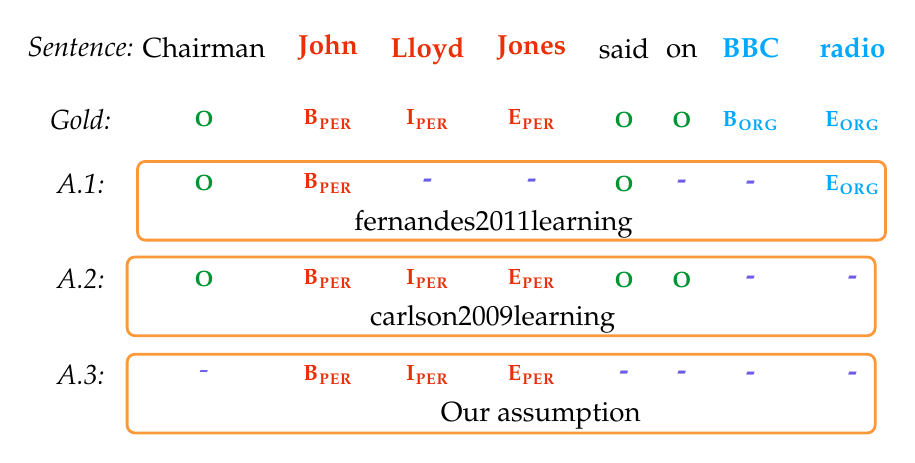
\begin{tikzpicture}[node distance=1.0mm and 4.0mm, >=Stealth, 
		word/.style={draw=none, minimum height=5mm, rectangle, inner sep=0pt},
		citationbox/.style={draw=puffin, rectangle, minimum height=10mm, minimum width=95mm,line width=1pt, fill=none, text=black,rounded corners=1mm}
		]
		\node [word] (sent) {\it Sentence: };
		\node [word, right= of sent, xshift=-3mm] (chairman) {Chairman};
		\node [word, right= of chairman, color=myred] (john) {\textbf{John}};
		\node [word, right= of john, yshift=-0.5mm, color=myred] (lloyd) {\textbf{Lloyd}};
		\node [word, right= of lloyd, yshift=0.4mm, color=myred] (jones) {\textbf{Jones}};
		\node [word, right= of jones] (said) {said};
		\node [word, right= of said, xshift=-2mm, yshift=-0.4mm] (on) {on};
		\node [word, right= of on, xshift=-1mm, yshift=0.4mm, color=myblue] (bbc) {\textbf{BBC}};
		\node [word, right= of bbc, xshift=1mm, color=myblue] (radio) {\textbf{radio}};
		
		\node[word, below= of sent, yshift=-3mm] (goldo) {\it Gold: };
		\node[word, below= of chairman, yshift=-3mm, color=grass] (l1) {{\textbf{\textsc{o}}}};
		\node[word, below= of john, yshift=-3mm, color=myred] (l2) {{\textbf{\textsc{b}$_{\textsc{per}}$}}};
		\node[word, below= of lloyd, yshift=-2.5mm, color=myred] (l3) {{\textbf{\textsc{i}$_{\textsc{per}}$}}};
		\node[word, below= of jones, yshift=-2.9mm, color=myred] (l4) {{\textbf{\textsc{e}$_{\textsc{per}}$}}};
		\node[word, below= of said, yshift=-3mm, color=grass] (l5) {{\textbf{\textsc{o}}}};
		\node[word, below= of on, yshift=-2.6mm, color=grass] (l6) {{\textbf{\textsc{o}}}};
		\node[word, below= of bbc, yshift=-3.1mm, color=myblue] (l7) {{\textbf{\textsc{b}$_{\textsc{org}}$}}};
		\node[word, below= of radio, yshift=-3.1mm, color=myblue] (l8) {{\textbf{\textsc{e}$_{\textsc{org}}$}}};
		
		\node[word, below= of goldo, yshift=-2mm] (a1) {\it A.1:};
		\node[word, below= of l1, yshift=-2mm, color=grass] (p1) {{\textbf{\textsc{o}}}};
		\node[word, below= of l2, yshift=-2mm, color=myred] (p2) {{\textbf{\textsc{b}$_{\textsc{per}}$}}};
		\node[word, below= of l3, yshift=-2mm, color=mypurple] (p3) {{\textbf{-}}};
		\node[word, below= of l4, yshift=-2mm, color=mypurple] (p4) {\textbf{-}};
		\node[word, below= of l5, yshift=-2mm, color=grass] (p5) {\textbf{\textsc{o}}};
		\node[word, below= of l6, yshift=-2mm, color=mypurple] (p6) {\textbf{-}};
		\node[word, below= of l7, yshift=-2mm, color=mypurple] (p7) {\textbf{-}};
		\node[word, below= of l8, yshift=-2mm, color=myblue] (p8) {\textbf{\textsc{e}$_{\textsc{org}}$}};
		
		\node[word, below right= of p2, yshift=1mm, xshift=-4mm] (c1) {\cite{fernandes2011learning}};
		\node [citationbox, left= of p8, xshift=12mm, yshift=-2mm, text depth=-0.6cm] (c1box) {};
		
		\node[word, below= of a1, yshift=-6mm] (a2) {\it A.2: };
		\node[word, below= of p1, yshift=-6mm, color=grass] (mx1) {\textbf{\textsc{o}}};
		\node[word, below= of p2, yshift=-6mm, color=myred] (mx2) {\textbf{\textsc{b}$_{\textsc{per}}$}};
		\node[word, below= of p3, yshift=-6mm, color=myred] (mx3) {\textbf{\textsc{i}$_{\textsc{per}}$}};
		\node[word, below= of p4, yshift=-6mm, color=myred] (mx4) {\textbf{\textsc{e}$_{\textsc{per}}$}};
		\node[word, below= of p5, yshift=-6mm, color=grass] (mx5) {\textbf{\textsc{o}}};
		\node[word, below= of p6, yshift=-6mm, color=grass] (mx6) {\textbf{\textsc{o}}};
		\node[word, below= of p7, yshift=-6mm, color=mypurple] (mx7) {\textbf{-}};
		\node[word, below= of p8, yshift=-6mm, color=mypurple] (mx8) {\textbf{-}};
		
		\node[word, below right= of mx2, yshift=1mm, xshift=-2mm] (c1) {\cite{carlson2009learning}};
		\node [citationbox, left= of mx8, xshift=7.7mm, yshift=-2mm, text depth=-0.6cm] (c2box) {};
		
		\node[word, below= of a2, yshift=-6mm] (a3) {\it A.3: };
		\node[word, below= of mx1, yshift=-6mm, color=mypurple] (px1) {{\textcolor{mypurple}{-}}};
		\node[word, below= of mx2, yshift=-6mm, color=myred] (px2) {\textbf{\textsc{b}$_{\textsc{per}}$}};
		\node[word, below= of mx3, yshift=-6mm, color=myred] (px3) {\textbf{\textsc{i}$_{\textsc{per}}$}};
		\node[word, below= of mx4, yshift=-6mm, color=myred] (px4) {\textbf{\textsc{e}$_{\textsc{per}}$}};
		\node[word, below= of mx5, yshift=-6mm, color=mypurple] (px5) {\textbf{-}};
		\node[word, below= of mx6, yshift=-6mm, color=mypurple] (px6) {\textbf{-}};
		\node[word, below= of mx7, yshift=-6mm, color=mypurple] (px7) {\textbf{-}};
		\node[word, below= of mx8, yshift=-6mm, color=mypurple] (px8) {\textbf{-}};
		
		\node[word, below right= of px2, yshift=1mm, xshift=7mm] (c3) {Our assumption};
		\node [citationbox, below= of c2box, yshift=-1mm] (c3box) {};
		
		\end{tikzpicture}
%	}
	%	\vspace{-7mm}
	\caption{An example sentence with gold named entity annotations and different assumptions (i.e., \textit{A.1} to \textit{A.3}) on {\em available labels}. ``\textsc{-}'' represents a missing label.}
	%	\vspace{-4.5mm}
	\label{fig:example1}
\end{figure}



Several previous approaches assume the incomplete annotations can be obtained by simply removing either word-level labels \cite{fernandes2011learning} or span-level labels \cite{carlson2009learning}. 
%	As shown in Figure \ref{fig:example1}, both assumptions (i.e., {\it A.1} and {\it A.2}) would result in words annotated with \textsc{o} labels. The former approach may even lead to sub-entity level annotations (e.g., ``{\em radio}'' is annotated as part of an entity).
As shown in Figure \ref{fig:example1}, under both assumptions (i.e., {\it A.1} and {\it A.2}), there will be words annotated with \textsc{o} labels. The former approach may even lead to sub-entity level annotations (e.g., ``{\em radio}'' is annotated as part of an entity).
However, we argue such assumptions can be largely unrealistic.
In practice, annotators are typically instructed to annotate named entities for complete word spans only~\cite{settles2008active,surdeanu2010legal}.
Thus, sub-entity level annotations or \textsc{o} labels \footnote{Why should the \textsc{o} labels be assumed unavailable? This is because  the annotators typically do not actively specify the \textsc{o} labels when working on annotations. If the annotator chooses not to annotate a word, it could either mean it is not part of any entity, {\em or} the word is actually part of an entity but the annotator neglected it in the annotation process (therefore we have incomplete annotations). However, we note that assigning the \textsc{o} label to a word would precisely indicate it is strictly {\em not} part of any entity, which is not desirable.} should not be assumed to be available ({\it A.3}).
Therefore such approaches are making sub-optimal assumptions on the {\em available labels}.





%\citet{fernandes2011learning} assume the incomplete annotations can be obtained by simply discarding some labels from the original gold label sequence.
%As we can see, such an approach may lead to incomplete entities such as ``{\em radio}''. We believe this is not a very realistic setup as in practice the annotators do not provide such sub-entity level annotations.
%\citet{carlson2009learning} approached this problem based on an alternative setup where the labels associated with certain complete entities are missing but \textsc{o} labels are still available.
%However, we note that in practice annotators are typically instructed to annotate entity spans only, ignoring a significant amount of other words in the text. 
%Thus, assuming the availability of \textsc{o} labels that indicate non-entities may be unrealistic as the annotators will not be actively assigning such labels to words.
%As we can see both approaches have limitations associated with their assumptions on the {\em annotated labels}.

When the proper assumptions on the available labels are made, one can typically model the missing labels as latent variables and train a latent-variable conditional random fields model \cite{quattoni2005conditional}.
One such approach is presented in \cite{bellare2007learning}.
Their work focused on the citation parsing\footnote{The task is to tag the BibTex records with different labels (i.e., ``title'', ``author'', ``affiliation'' and so on).} (i.e., sequence labeling) task which does not suffer from the above issue as no \textsc{o} label is involved.
However, though the approach was shown effective in the citation parsing task, we found its effectiveness does not transfer to the NER task even in the absence of the above {available labels} issue.
As we would highlight later, the reason is related to the undesirable assumptions on the {\em unavailable labels}.
%Our further investigations lead to the important notion of {\em latent label distribution} for unlabeled words, to which we provide more details in Section \ref{sec:problem}.
%\citet{bellare2007learning} presented a more realistic setup where the only labels available are those assigned to the entities, as also illustrated in Figure \ref{fig:example1}. They proposed to use a latent-variable conditional random fields (CRF)  model \cite{lafferty2001conditional} to learn the underlying distributions of unavailable labels in the sentence.
%However, while their approach was shown to be effective in the citation parsing task, we found their approach in practice does not work well in the context of NER.
%Our investigations show that this issue is mainly attributed to their assumptions made on the {\em unavailable labels}.
%We tackle this issue by defining the {\em latent label distribution} in Section \ref{luwei:provide section name}.

%In this work, we investigate the issue and highlight the importance of correctly specifying the {\em latent label distribution}, which is especially crucial for the task of NER due to the special nature of such a task.
%We show that the partial CRF approach in fact exploits a simple uniform distribution as their latent label distribution for such a task, whereas our approach is able to provide a more sensible estimation for the latent label distribution.
%, and can lead to significantly better results.

%There are already several approaches that tackle the incomplete data annotation problem. The work of \cite{} presented 
%One of the first questions is what is the more realistic scenario associated with modeling the incomplete annotation. - previous approaches are wrong.

%There are existing approaches that address the incomplete data annotation issue. 
%One notable approach is the the partial CRF model of \cite{bellare2007learning,carlson2009learning}.
%The model is a general approach designed for sequence labeling where the assumption is there are missing labels.
%The true underlying labels are then regarded as latent variables in the training phase. 
%The resulting model is essentially a latent variable CRF -- an approach that has been used in various other applications such as syntactic parsing \cite{petrov-klein:2008:EMNLP}, semantic parsing \cite{Zettlemoyer:2005:LMS:3020336.3020416} and statistical machine translation \cite{blunsom2008discriminative}.

%While such an approach yields reasonable results, we note that the task of named entity recognition has certain special characteristics that distinguish it from many other sequence labeling problems such as Chinese word segmentation and part-of-speech tagging.
%One key observation that we make here is that the named entity recognition task is essentially an {\em unbalanced labeling} problem while many other tasks involve {\em balanced labeling} problem.
%The difference between the two types of problems is, when we cast the problem of named entity recognition as a sequence labeling problem, the annotators typically actively mark the boundaries of entities, assuming the remaining words are assigned the default label \textsc{o} (indicating the word is outside of any entity).

%We call the former  {\em balanced labeling} problem and the latter {\em unbalanced labeling} problem.
%Unfortunately, existing approaches largely focused on the former setup and largely ignored the second setup.
%However, we note that the second setup is more natural and realistic.
%This is because in the annotation process, the annotator typically only actively search for relevant entities and ignore the irrelevant text.
%If a certain text span is ignored, it is usually regarded as irrelevant text and are therefore labeled as \text{o}.
%However, in the event of missing annotations, if a certain text span is not assigned any annotation, there are essentially two possibilities: whether it is o or it is part of an entity but is neglected by the annotator.
%However, in the common setup used in partial CRF, the assumption was many tags are not available. We believe this is not a very realistic setup as in practice the annotators do not actively specify the o tags.
%We present a more realistic setup in practice. 

%In the sequence labeling tasks, we need to predict a label for each token in the input sequence. 
%Partial data annotation in sequence labeling often refers to the missing label information for some tokens in the sequence. 
%Figure \ref{fig:example1} shows an example of two input sequences and each with three corresponding label sequences: POS tags, named entities and sentiment labels. 
%Labels that colored in red are the annotations observed and those colored in blue are not observed under the partial data annotation setting. 
%In this case, we only have the knowledge that ``\textit{Steve}'' is a ``\textsc{Person}'' (\textsc{Per}) entity during the training phase in the NER task. 
%Similar in the second sentence, we can only observe the ``\textit{kimchi}'' is an ``\textsc{Misc}'' entity. 
%The named entity and sentiment label sequences are dominated by the label \textsc{O} (i.e., non-entity) while the POS tag sequence is dominated by any labels. 
%Based on this observation, we categorize sequences like named entities and sentiment labels as ``\textit{unbalanced label sequences}'' and sequences like POS tags as ``\textit{balanced label sequences}''. 
%The label sequences in other tasks such as chunking and Chinese word segmentation~\cite{sun2011enhancing} also refer as ``\textit{balanced label sequences}''. 
%Previous work has shown promising performance on balanced label sequences, such as POS tagging with partial data annotations especially in low-resource language~\cite{tsuboi-EtAl:2008:PAPERS,garrette2012type,garrette2013real,garrette2013learning} and Chinese word segmentation with partially labeled data~\cite{yang2014semi,liu-EtAl:2014:EMNLP2014}. 
%
%In this work, we specifically focus on partial data annotations on the ``\textit{unbalanced label sequence}'' that is present in the task of named entity recognition. 
%Previous work~\cite{carlson2009learning,fernandes2011learning} solved the problem with partial annotations under a setup where the token labels are randomly removed. 
%Unlike previous work, we focus on a more challenging and realistic setup where the information of the dominated label (i.e., \textsc{O} label in our case) is always unknown and the entity (or targeted sentiment) labels are randomly removed. 
%In practice, annotators are often asked to annotate what are the specific entities based on specific requirements. 
%For example, annotators can be asked to annotate the entities with ``\textit{brand}'' while there are still ``\textit{material}'' entities in the sentences. 
%Under this challenging setup, we analyze and empirically show the difficulties for traditional models such as partial conditional random fields (CRF). 
%They might suffer from unbalanced label issue when we have no \textsc{O} type annotations at all. 
%The annotations for \textsc{O} types and other entity labels are all unknown though most of the tokens should be labeled as \textsc{O}. 
%Common sequence labeling models such as conditional random fields (CRF) probably try to predict most of the tokens as entities as we do not have any \textsc{O} type annotations in the training data at all. 
%Inspired by \newcite{dredze2009sequence}, we then propose our bootstrapping CRF model to attack the difficulties by splitting the datasets into multiple parts and applying estimation distribution on the unlabeled tokens. 
%The estimation distribution is trained on some parts of the dataset and then applied on the other part of the dataset. 

In this work, we tackle the incomplete annotation problem when building an NER system, under a more realistic yet more challenging scenario. 
We present a novel, effective, yet easy-to-implement approach, and conduct extensive experiments on various datasets and show our approach significantly outperforms several previous approaches.

%In this work, we resolve both of the above issues and propose a better approach for modeling incomplete annotation for the task of named entity recognition.
%Specifically, we make the following major contributions:
%\squishlist
%\item We tackle the incomplete annotation problem under a challenging yet more realistic scenario for learning named entity recognition systems.
%% from incomplete annotation.
%%\item We present the difficulties of a challenging partial data annotation problem for traditional models. 
%\item We present a novel, effective, yet easy-to-implement approach for NER with incomplete data annotation based on our practical setup.
%%\item We propose a self-learning model for sequence labeling with partial data annotation. The proposed approach makes use of the advantages of multiple parts of datasets and performs self training to improve the performance. 
%\item We conduct extensive experiments on various datasets and show our approach \footnote{Our code will be made available for download.} significantly outperforms several previous approaches.

%\item Extensive experiments conducted on the five datasets prove the effectiveness of the proposed approach\footnote{Our code will be released under *URL*}. 
%\squishend


\section{Related Work}
Previous research efforts on partially annotated data are mostly based on the conditional random fields (CRF)~\cite{lafferty2001conditional}, structured perceptron~\cite{collins2002discriminative} and max-margin~\cite{tsochantaridis2005large} (e.g. structural support vector machine) models.
%	 (i.e., structured perceptron and support vector machines). 
\citet{bellare2007learning} proposed a missing label linear-chain CRF\footnote{This model was also named as Partial CRF~\cite{carlson2009learning} and EM Marginal CRF~\cite{greenberg2018marginal}.} which is essentially a latent-variable CRF~\cite{quattoni2005conditional} on citation parsing~\cite{mccallum2000automating}.
This model had also been used in part-of-speeching tagging and segmentation task with incomplete annotations~\cite{tsuboi-EtAl:2008:PAPERS, liu-EtAl:2014:EMNLP2014,yang2014semi}. 
\citet{yang2018distantly} showed the effectiveness of such a model on Chinese NER with incomplete annotations due to the fact that they required a certain number of fully annotated data to perform joint training. 
\citet{greenberg2018marginal} applied this model on a biomedical NER task and achieved promising performance with incomplete annotations. 
However, in their assumption for the incomplete annotations, the \textsc{O} labels are still considered, which we believe is not realistic. 
%	achieved promising performance on the biomedical NER task with this model but {\color{red}their assumption largely reduces the number of {\it unavailable labels}}. 
\citet{carlson2009learning} modified the structured perceptron algorithm and defined features only on the tokens with annotated labels in partially labeled sequences. 
\citet{fernandes2011learning} and \citet{lou2012structured} proposed to use a large-margin learning framework similar to structured support vector machines with latent variables~\cite{yu2009learning}. 




\section{Approach}
\label{sec:problem}

Given the input word sequence $\vec{x}$, the NER task is to predict a label sequence $\vec{y}$ that encodes the NER information (e.g., in a form following the \textsc{bioes} tagging scheme). Given a training set that consists of completely labeled data $\mathcal{D}$, one can tackle this problem using a standard linear-chain conditional random field (CRF) \cite{lafferty2001conditional} whose loss function is as follows:\footnote{In practice, we also have an $L_2$ regularization term, which we exclude from the formula for brevity.}
\begin{equation}
\mathcal{L}(\vec{w}) 
=
-
\sum_{i}
\log
p_{\vec{w}} (\vec{y}^{(i)} \vert \vec{x}^{(i)}) 
\end{equation}
%	\begin{center}
%		\begin{tabular}{c}
%			$
%				\mathcal{L}(\vec{w}) 
%			=
%			-
%			\sum_{i}
%			\log
%			p_{\vec{w}} (\vec{y}^{(i)} \vert \vec{x}^{(i)}) 
%			$
%		\end{tabular}
%		%\vspace{-2mm}
%	\end{center}
where $(\mathbf{x}^{(i)}, \mathbf{y}^{(i)})$ is the $i$-th instance from $\mathcal{D}$. 
%	, $\kappa$ is the $\ell_2$ coefficient and $\mathbf{w}$  the model parameters.
%$p_{\mathbf{w}}(\mathbf{y}|\mathbf{x})$ can be parameterized as:
%\begin{align}
%p_\vec{w} (\vec{y}|\vec{x}) 
%= \frac{\exp(\vec{w}\cdot\vec{f}(\vec{x}, \vec{y}))}{\sum_{\vec{y}'} \exp(\vec{w}\cdot\vec{f}(\vec{x}, \vec{y}'))} 
%\end{align}

%We can also rewrite the above function as:
%% in the following form:
%\begin{align}
%%\mathcal{L}(\vec{w}) 
%%=& 
%-\sum_{i}
%\log
%\sum_{ \vec{y} } 
%q_{\mathcal{D}} (\vec{y} | \vec{x}^{(i)}) 
%p_{\vec{w}} (\vec{y} \vert \vec{x}^{(i)}) 
%%\nonumber\\
%%&
%\label{equ:finalobj2}
%\end{align}
%where $q_{\mathcal{D}} (\vec{y} | \vec{x}^{(i)})$ will be an indicator function that returns 1 if and only if $\mathbf{y}=\mathbf{y}^{(i)}$.
%Note that in the above function $\mathbf{y}$ or $\mathbf{y}^{(i)}$ are assumed to be complete label sequences. 

%%%%%%%% BEGIN OF 4 FIGURES %%%%%%%

%%%%%%%% BEGIN OF 4 FIGURES %%%%%%%
\begin{figure*}[h!]
	%		\centering
	\begin{subfigure}{0.5\textwidth}
		\centering
		\scalebox{0.5}{
			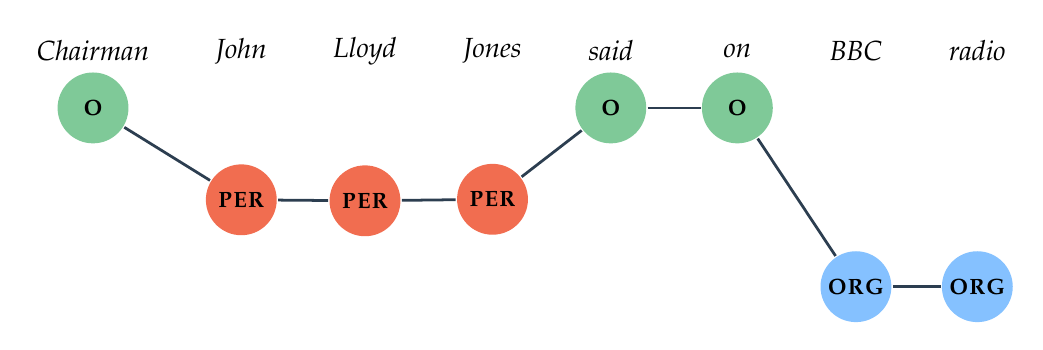
\begin{tikzpicture}[node distance=2.0mm and 6.0mm, >=Stealth, 
			word/.style={draw=none, minimum height=5mm, rectangle},
			olabel/.style={draw=none, circle, minimum height=9mm, minimum width=9mm,line width=1pt, inner sep=2pt, fill=grass, text=fontgray, label={center:\textbf{\textsc{o}}}, fill opacity=0.5},
			bperlabel/.style={draw=none, circle, minimum height=9mm, minimum width=9mm,line width=1pt, inner sep=2pt, fill=myred, text=black, label={center:\textbf{\textsc{per}}}, fill opacity=0.7},
			borglabel/.style={draw=none, circle, minimum height=9mm, minimum width=9mm,line width=1pt, inner sep=2pt, fill=lowblue, text=black, label={center:\textbf{\textsc{org}}}, fill opacity=0.8},
			invis/.style={draw=none, circle, minimum height=9mm, minimum width=9mm,line width=1pt, inner sep=2pt, fill=none, text=fontgray},
			chainLine/.style={line width=1pt,-, color=fontgray}	%		,background rectangle/.style={fill=olive!45}, show background rectangle
			]
			\node[word](p0) [] {\it Chairman};
			\node[word](p1) [right = of p0] {\it John};
			\node[word](p2) [right = of p1] {\it Lloyd};
			\node[word](p3) [right = of p2] {\it Jones};
			\node[word](p4) [right = of p3] {\it said};
			\node[word, xshift=3mm](p5) [right = of p4] {\it on};
			\node[word, xshift=1.5mm](p6) [right = of p5] {\it BBC};
			\node[word](p7) [right = of p6] {\it radio};
			\node[olabel](t0o) [below = of p0, yshift=2mm] {};
			\node[invis](t0bper) [below = of t0o] {};
			%			\node[word](graphlabel) [left = of t0bper, xshift=-2mm] {\Large (a) {\it Gold}};
			
			\node[invis](t1o) [below = of p1, yshift=2mm] {};
			\node[bperlabel](t1per) [below = of t1o] {};
			
			\node[invis](t2o) [below = of p2, yshift=2mm] {};
			\node[bperlabel](t2per) [below = of t2o] {};
			
			\node[invis](t3o) [below = of p3, yshift=2mm] {};
			\node[bperlabel](t3per) [below = of t3o] {};
			
			\node[olabel](t4o) [below = of p4, yshift=2mm] {};
			
			\node[olabel](t5o) [below = of p5, yshift=2mm] {};
			
			\node[invis](t6o) [below = of p6, yshift=2mm] {};
			\node[invis](t6per) [below = of t6o] {};
			\node[borglabel](t6org) [below = of t6per] {};
			
			\node[invis](t7o) [below = of p7, yshift=2mm] {};
			\node[invis](t7per) [below = of t7o] {};
			\node[borglabel](t7org) [below = of t7per] {};
			
			
			\begin{pgfonlayer}{background}
			\draw [chainLine] (t0o) to (t1per);
			\draw [chainLine] (t1per) to (t2per);
			\draw [chainLine] (t2per) to (t3per);
			\draw [chainLine] (t3per) to (t4o);
			\draw [chainLine] (t4o) to (t5o);
			\draw [chainLine] (t5o) to (t6org);
			\draw [chainLine] (t6org) to (t7org);
			\end{pgfonlayer}
			
			
			
			\end{tikzpicture}
		}
		%			\vspace{-4mm}
		%			\caption{\em Gold}
		\label{fig:groundtruth}
		\caption{\textit{Gold}}
	\end{subfigure}
	\begin{subfigure}{0.5\textwidth}
		\centering
		\scalebox{0.5}{
			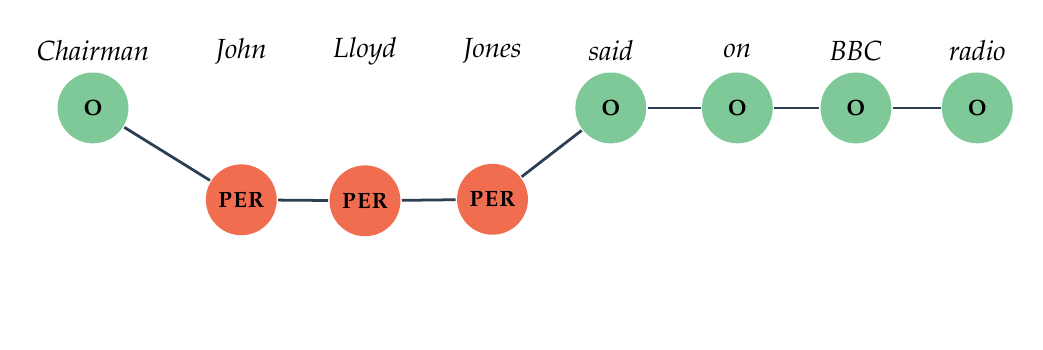
\begin{tikzpicture}[node distance=2.0mm and 6.0mm, >=Stealth, 
			word/.style={draw=none, minimum height=5mm, rectangle},
			olabel/.style={draw=none, circle, minimum height=9mm, minimum width=9mm,line width=1pt, inner sep=2pt, fill=grass, text=fontgray, label={center:\textbf{\textsc{o}}}, fill opacity=0.5},
			bperlabel/.style={draw=none, circle, minimum height=9mm, minimum width=9mm,line width=1pt, inner sep=2pt, fill=myred, text=black, label={center:\textbf{\textsc{per}}}, fill opacity=0.7},
			borglabel/.style={draw=none, circle, minimum height=9mm, minimum width=9mm,line width=1pt, inner sep=2pt, fill=lowblue, text=black, label={center:\textbf{\textsc{org}}}, fill opacity=0.8},
			invis/.style={draw=none, circle, minimum height=9mm, minimum width=9mm,line width=1pt, inner sep=2pt, fill=none, text=fontgray},
			chainLine/.style={line width=1pt,-, color=fontgray}	%		,background rectangle/.style={fill=olive!45}, show background rectangle
			]
			\node[word](p0) [] {\it Chairman};
			\node[word](p1) [right = of p0] {\it John};
			\node[word](p2) [right = of p1] {\it Lloyd};
			\node[word](p3) [right = of p2] {\it Jones};
			\node[word](p4) [right = of p3] {\it said};
			\node[word, xshift=3mm](p5) [right = of p4] {\it on};
			\node[word, xshift=1.5mm](p6) [right = of p5] {\it BBC};
			\node[word](p7) [right = of p6] {\it radio};
			\node[olabel](t0o) [below = of p0, yshift=2mm] {};
			\node[invis](t0bper) [below = of t0o, yshift=2mm] {};
			%			\node[word](graphlabel) [left = of t0bper, xshift=3mm] {\Large (b) {\it Simple}};
			
			\node[invis](t1o) [below = of p1, yshift=2mm] {};
			\node[bperlabel](t1per) [below = of t1o] {};
			
			\node[invis](t2o) [below = of p2, yshift=2mm] {};
			\node[bperlabel](t2per) [below = of t2o] {};
			
			\node[invis](t3o) [below = of p3, yshift=2mm] {};
			\node[bperlabel](t3per) [below = of t3o] {};
			
			\node[olabel](t4o) [below = of p4, yshift=2mm] {};
			
			\node[olabel](t5o) [below = of p5, yshift=2mm] {};
			
			\node[olabel](t6o) [below = of p6, yshift=2mm] {};
			\node[invis](t6per) [below = of t6o] {};
			\node[invis](t6org) [below = of t6per] {};
			
			\node[olabel](t7o) [below = of p7, yshift=2mm] {};
			\node[invis](t7per) [below = of t7o] {};
			\node[invis](t7org) [below = of t7per] {};
			
			\begin{pgfonlayer}{background}
			\draw [chainLine] (t0o) to (t1per);
			\draw [chainLine] (t1per) to (t2per);
			\draw [chainLine] (t2per) to (t3per);
			\draw [chainLine] (t3per) to (t4o);
			\draw [chainLine] (t4o) to (t5o);
			\draw [chainLine] (t5o) to (t6o);
			\draw [chainLine] (t6o) to (t7o);
			
			
			\end{pgfonlayer}
			\end{tikzpicture}
		}
		%		\vspace{-4mm}
		%			\caption{\textit{Simple}}
		%			\vspace{-1mm}
		\caption{\textit{Simple}}
	\end{subfigure}
	%	\vspace{-5mm}
\end{figure*}
\begin{figure*}[h!]
	\begin{subfigure}{0.5\textwidth}
		\centering
		\scalebox{0.5}{
			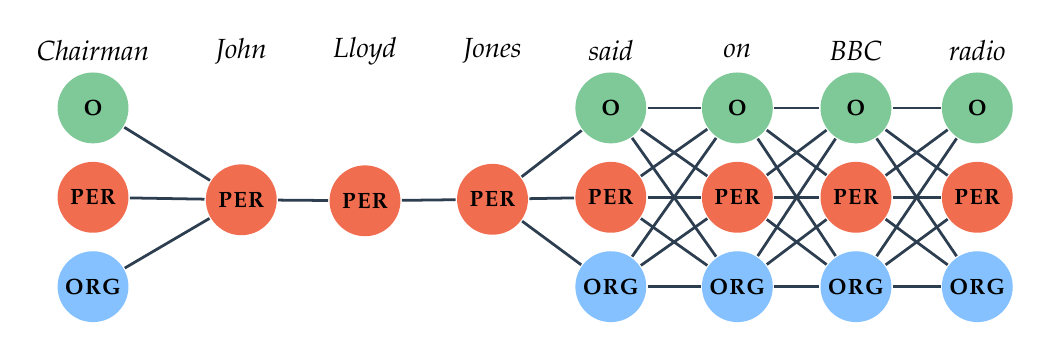
\begin{tikzpicture}[node distance=2.0mm and 6.0mm, >=Stealth, 
			word/.style={draw=none, minimum height=5mm, rectangle},
			olabel/.style={draw=none, circle, minimum height=9mm, minimum width=9mm,line width=1pt, inner sep=2pt, fill=grass, text=fontgray, label={center:\textbf{\textsc{o}}}, fill opacity=0.5},
			bperlabel/.style={draw=none, circle, minimum height=9mm, minimum width=9mm,line width=1pt, inner sep=2pt, fill=myred, text=black, label={center:\textbf{\textsc{per}}}, fill opacity=0.7},
			borglabel/.style={draw=none, circle, minimum height=9mm, minimum width=9mm,line width=1pt, inner sep=2pt, fill=lowblue, text=black, label={center:\textbf{\textsc{org}}}, fill opacity=0.8},
			invis/.style={draw=none, circle, minimum height=9mm, minimum width=9mm,line width=1pt, inner sep=2pt, fill=none, text=fontgray},
			chainLine/.style={line width=1pt,-, color=fontgray}	%		,background rectangle/.style={fill=olive!45}, show background rectangle
			]
			\node[word](p0) [] {\it Chairman};
			\node[word](p1) [right = of p0] {\it John};
			\node[word](p2) [right = of p1] {\it Lloyd};
			\node[word](p3) [right = of p2] {\it Jones};
			\node[word](p4) [right = of p3] {\it said};
			\node[word, xshift=3mm](p5) [right = of p4] {\it on};
			\node[word, xshift=1.5mm](p6) [right = of p5] {\it BBC};
			\node[word](p7) [right = of p6] {\it radio};
			
			\node[olabel](t0o) [below = of p0, yshift=2mm] {};
			\node[bperlabel](t0per) [below = of t0o] {};
			\node[borglabel](t0org) [below = of t0per] {};
			
			%			\node[word](graphlabel) [left = of t0bper, xshift=5mm] {\Large (c) {\it Uniform}};
			
			\node[invis](t1o) [below = of p1, yshift=2mm] {};
			\node[bperlabel](t1per) [below = of t1o] {};
			
			\node[invis](t2o) [below = of p2, yshift=2mm] {};
			\node[bperlabel](t2per) [below = of t2o] {};
			
			\node[invis](t3o) [below = of p3, yshift=2mm] {};
			\node[bperlabel](t3per) [below = of t3o] {};
			
			\node[olabel](t4o) [below = of p4, yshift=2mm] {};
			\node[bperlabel](t4per) [below = of t4o] {};
			\node[borglabel](t4org) [below = of t4per] {};
			
			\node[olabel](t5o) [below = of p5, yshift=2mm] {};
			\node[bperlabel](t5per) [below = of t5o] {};
			\node[borglabel](t5org) [below = of t5per] {};
			
			\node[olabel](t6o) [below = of p6, yshift=2mm] {};
			\node[bperlabel](t6per) [below = of t6o] {};
			\node[borglabel](t6org) [below = of t6per] {};
			
			\node[olabel](t7o) [below = of p7, yshift=2mm] {};
			\node[bperlabel](t7per) [below = of t7o] {};
			\node[borglabel](t7org) [below = of t7per] {};
			
			
			\begin{pgfonlayer}{background}
			
			\draw [chainLine] (t0o) to (t1per);
			\draw [chainLine] (t0per) to (t1per);
			\draw [chainLine] (t0org) to (t1per);
			
			\draw [chainLine] (t1per) to (t2per);
			\draw [chainLine] (t2per) to (t3per);
			
			\draw [chainLine] (t3per) to (t4o);
			\draw [chainLine] (t3per) to (t4per);
			\draw [chainLine] (t3per) to (t4org);
			
			\draw [chainLine] (t4o) to (t5o);
			\draw [chainLine] (t4o) to (t5per);
			\draw [chainLine] (t4o) to (t5org);
			\draw [chainLine] (t4per) to (t5o);
			\draw [chainLine] (t4per) to (t5per);
			\draw [chainLine] (t4per) to (t5org);
			\draw [chainLine] (t4org) to (t5o);
			\draw [chainLine] (t4org) to (t5per);
			\draw [chainLine] (t4org) to (t5org);
			
			\draw [chainLine] (t5o) to (t6o);
			\draw [chainLine] (t5o) to (t6per);
			\draw [chainLine] (t5o) to (t6org);
			\draw [chainLine] (t5per) to (t6o);
			\draw [chainLine] (t5per) to (t6per);
			\draw [chainLine] (t5per) to (t6org);
			\draw [chainLine] (t5org) to (t6o);
			\draw [chainLine] (t5org) to (t6per);
			\draw [chainLine] (t5org) to (t6org);
			
			\draw [chainLine] (t6o) to (t7o);
			\draw [chainLine] (t6o) to (t7per);
			\draw [chainLine] (t6o) to (t7org);
			\draw [chainLine] (t6per) to (t7o);
			\draw [chainLine] (t6per) to (t7per);
			\draw [chainLine] (t6per) to (t7org);
			\draw [chainLine] (t6org) to (t7o);
			\draw [chainLine] (t6org) to (t7per);
			\draw [chainLine] (t6org) to (t7org);
			
			
			\end{pgfonlayer}
			
			
			
			\end{tikzpicture}
		}
		%			\vspace{-2mm}
		%			\caption{\em Uniform}
		\caption{\textit{Uniform}}
		\label{fig:unifrom}
	\end{subfigure}
	\begin{subfigure}{0.5\textwidth}
		\centering
		\scalebox{0.5}{
			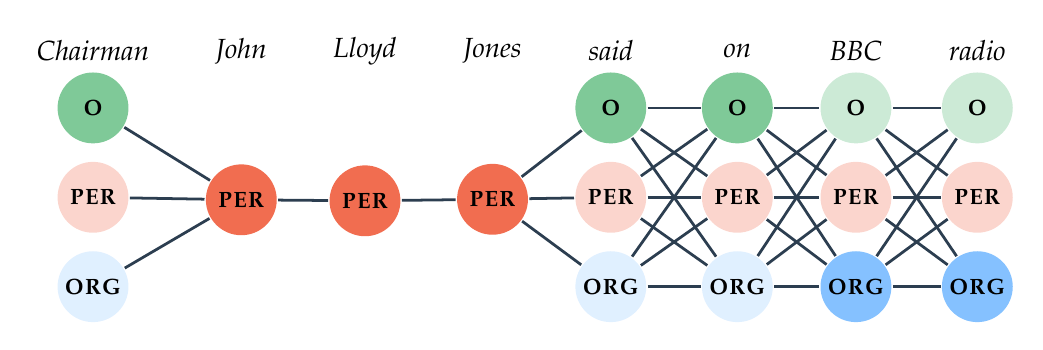
\begin{tikzpicture}[node distance=2.0mm and 6.0mm, >=Stealth, 
			word/.style={draw=none, minimum height=5mm, rectangle},
			olabel/.style={draw=none, circle, minimum height=9mm, minimum width=9mm,line width=1pt, inner sep=2pt, fill=grass, text=fontgray, label={center:\textbf{\textsc{o}}}, fill opacity=0.5},
			bperlabel/.style={draw=none, circle, minimum height=9mm, minimum width=9mm,line width=1pt, inner sep=2pt, fill=myred, text=black, label={center:\textbf{\textsc{per}}}, fill opacity=0.7},
			borglabel/.style={draw=none, circle, minimum height=9mm, minimum width=9mm,line width=1pt, inner sep=2pt, fill=lowblue, text=black, label={center:\textbf{\textsc{org}}}, fill opacity=0.8},
			invis/.style={draw=none, circle, minimum height=9mm, minimum width=9mm,line width=1pt, inner sep=2pt, fill=none, text=fontgray},
			chainLine/.style={line width=1pt,-, color=fontgray}	%		,background rectangle/.style={fill=olive!45}, show background rectangle
			]
			\node[word](p0) [] {\it Chairman};
			\node[word](p1) [right = of p0] {\it John};
			\node[word](p2) [right = of p1] {\it Lloyd};
			\node[word](p3) [right = of p2] {\it Jones};
			\node[word](p4) [right = of p3] {\it said};
			\node[word, xshift=3mm](p5) [right = of p4] {\it on};
			\node[word, xshift=1.5mm](p6) [right = of p5] {\it BBC};
			\node[word](p7) [right = of p6] {\it radio};
			
			\node[olabel](t0o) [below = of p0, yshift=2mm] {};
			\node[bperlabel, fill opacity=0.2](t0per) [below = of t0o] {};
			\node[borglabel, fill opacity=0.2](t0org) [below = of t0per] {};
			%			\node[word](graphlabel) [left = of t0bper, xshift=-1mm] {\Large (d) {\it Ours}};
			
			\node[invis](t1o) [below = of p1, yshift=2mm] {};
			\node[bperlabel](t1per) [below = of t1o] {};
			
			\node[invis](t2o) [below = of p2, yshift=2mm] {};
			\node[bperlabel](t2per) [below = of t2o] {};
			
			\node[invis](t3o) [below = of p3, yshift=2mm] {};
			\node[bperlabel](t3per) [below = of t3o] {};
			
			\node[olabel](t4o) [below = of p4, yshift=2mm] {};
			\node[bperlabel, fill opacity=0.2](t4per) [below = of t4o] {};
			\node[borglabel, fill opacity=0.2](t4org) [below = of t4per] {};
			
			\node[olabel](t5o) [below = of p5, yshift=2mm] {};
			\node[bperlabel, fill opacity=0.2](t5per) [below = of t5o] {};
			\node[borglabel, fill opacity=0.2](t5org) [below = of t5per] {};
			
			\node[olabel, fill opacity=0.2](t6o) [below = of p6, yshift=2mm] {};
			\node[bperlabel, fill opacity=0.2](t6per) [below = of t6o] {};
			\node[borglabel](t6org) [below = of t6per] {};
			
			\node[olabel, fill opacity=0.2](t7o) [below = of p7, yshift=2mm] {};
			\node[bperlabel, fill opacity=0.2](t7per) [below = of t7o] {};
			\node[borglabel](t7org) [below = of t7per] {};
			
			\begin{pgfonlayer}{background}
			\draw [chainLine] (t0o) to (t1per);
			\draw [chainLine] (t0per) to (t1per);
			\draw [chainLine] (t0org) to (t1per);
			
			\draw [chainLine] (t1per) to (t2per);
			\draw [chainLine] (t2per) to (t3per);
			
			\draw [chainLine] (t3per) to (t4o);
			\draw [chainLine] (t3per) to (t4per);
			\draw [chainLine] (t3per) to (t4org);
			
			\draw [chainLine] (t4o) to (t5o);
			\draw [chainLine] (t4o) to (t5per);
			\draw [chainLine] (t4o) to (t5org);
			\draw [chainLine] (t4per) to (t5o);
			\draw [chainLine] (t4per) to (t5per);
			\draw [chainLine] (t4per) to (t5org);
			\draw [chainLine] (t4org) to (t5o);
			\draw [chainLine] (t4org) to (t5per);
			\draw [chainLine] (t4org) to (t5org);
			
			\draw [chainLine] (t5o) to (t6o);
			\draw [chainLine] (t5o) to (t6per);
			\draw [chainLine] (t5o) to (t6org);
			\draw [chainLine] (t5per) to (t6o);
			\draw [chainLine] (t5per) to (t6per);
			\draw [chainLine] (t5per) to (t6org);
			\draw [chainLine] (t5org) to (t6o);
			\draw [chainLine] (t5org) to (t6per);
			\draw [chainLine] (t5org) to (t6org);
			
			\draw [chainLine] (t6o) to (t7o);
			\draw [chainLine] (t6o) to (t7per);
			\draw [chainLine] (t6o) to (t7org);
			\draw [chainLine] (t6per) to (t7o);
			\draw [chainLine] (t6per) to (t7per);
			\draw [chainLine] (t6per) to (t7org);
			\draw [chainLine] (t6org) to (t7o);
			\draw [chainLine] (t6org) to (t7per);
			\draw [chainLine] (t6org) to (t7org);
			
			
			\end{pgfonlayer}
			
			\end{tikzpicture}
		}
		%			\vspace{-1mm}
		%			\caption{\em Ours}
		\caption{\textit{Ours}}
		\label{fig:ours}
	\end{subfigure}
	
	%		\vspace{-2mm}
	\caption{Graphical illustrations on different assumptions on {\em unavailable labels}, where the entity ``{\em John Lloyd Jones}'' of type \textsc{per} is labeled but ``{\em BBC radio}'' of type \textsc{org} is missing. Each path refers to one possible complete label sequence, and the density of the color indicates probability (we excluded \textsc{b} and \textsc{e} tags for brevity).}
	%		\vspace{-4mm}
	\label{fig:nerlabelseq}
\end{figure*}
%%%%%%%% END OF 4 FIGURES %%%%%%%
%%%%%%%% END OF 4 FIGURES %%%%%%%


Now, assume we have an incomplete label sequence $\mathbf{y}_p^{(i)}$. From such a $\mathbf{y}_p^{(i)}$ we should be able to derive a set of all possible complete label sequences that are compatible with (i.e., contain) the incomplete label sequence, and let us call this set $\mathcal{C}(\mathbf{y}_p^{(i)})$. 
%	Apparently, $\mathcal{C}(\mathbf{y}^{(i)})=\{\mathbf{y}^{(i)}\}$ for a complete label sequence $\mathbf{y}^{(i)}$. 
We can  rewrite the above function as:
%	\begin{center}
%		\begin{tabular}{c}
%			$
%			\mathcal{L}(\vec{w}) 
%			= 
%			-
%%			\!\!
%			\sum\limits_{i}
%			\log
%%			\!\!\!
%%			\!\!\!\!
%			\sum\limits_{ \vec{y}\in\mathcal{C}(\mathbf{y}^{(i)}_p) } 
%%			\!\!\!\!
%			q_{\mathcal{D}} (\vec{y} | \vec{x}^{(i)}) 
%			p_{\vec{w}} (\vec{y} \vert \vec{x}^{(i)}) 
%			$
%		\end{tabular}
%		%\vspace{-2mm}
%	\end{center}
\begin{align}
\mathcal{L}(\vec{w}) 
=& 
-
\sum_{i}
\log
\sum_{ \vec{y}\in\mathcal{C}(\mathbf{y}^{(i)}_p) } 
q_{\mathcal{D}} (\vec{y} | \vec{x}^{(i)}) 
p_{\vec{w}} (\vec{y} \vert \vec{x}^{(i)}) 
\nonumber
%&
\label{equ:finalobj3}
\end{align}

%	Understanding the loss function from such a perspective helps us establish a unified view of various approaches to learning with incomplete annotation.
%	Based on such a unified view we also develop our own approach.
%It is also helpful for developing our new approach.

We illustrate in Figure \ref{fig:nerlabelseq} several previous approaches as well as our approach. 
In this example, the entity {\em BBC radio} of type \textsc{org} is not annotated.
Figure \ref{fig:nerlabelseq}(a) shows a single path that corresponds to the gold label sequence.
Figure \ref{fig:nerlabelseq}(b) illustrates a naive approach, where we regard all the missing labels as \textsc{o} labels. 
This essentially assumes that the $q$ distribution in the above equation puts all probability mass to this single label sequence, which is an incorrect assumption.   
%	Unfortunately as we can see this is an incorrect assumption.

%We will use such a form to develop our approach when we have incomplete data annotation.
%The NER task is a sequence labeling problem, where we would like to predict a label sequence $\vec{y} = \{y_{1}, y_{2}, \cdots, y_{n}\}$ given an observation sequence $\vec{x} = \{x_{1}, x_{2}, \cdots, x_{n}\}$ where $n$ is the number of tokens in the sequence. 
%As the training data is partially annotated, each instance in the training set $\mathcal{D}$ is therefore represented as an ordered pair $(\vec{x}, \vec{y}_p)$ where $\vec{y}_p$ represents a partial label sequence. 
%As we conduct experiments on named entity recognition and targeted sentiment analysis, the label set is named entities and sentiment labels for two tasks, respectively. 
%Additionally, we use the \textsc{o} label to denote tokens that do not belong to entities.
% or sentiment classes.
%those tokens not labeled as entities or sentiment classes.  
%As we have seen in the previous sections, the label sequences both NER and entity-level sentiment analysis tasks are dominated by the $\mathbf{O}$ label. 
%We study the partial data annotation problem under a challenging setup during the training phase: 
%
%\begin{center}
%	\textit{Only a few (complete) entities are observed for each sentence, which means no annotation on $\mathbf{O}$ label is observed.}
%\end{center}
%
%In practice, we usually annotate the entity type information and sometimes only the specific entity type as only those are important for a specific dataset. 
%However, the dataset might contains other entity types which are not annotated but annotated in other datasets. 
%Our setup above indicates this scenario in practice. 
%For example in Figure \ref{fig:example1}, some might be interested in \textsc{per} entities only, thus the annotation only show the positions where we have the \textsc{per}. 



Now let us look at what assumptions on $q$ have been made by the existing approach of~\cite{bellare2007learning}.
The model regards the missing labels as latent variables and learns a latent variable CRF using the following loss:
%	\begin{center}
%		\begin{tabular}{c}
%			$
%				-\sum_{i}
%			\log
%			\sum_{ \vec{y}\in\mathcal{C}(\mathbf{y}^{(i)}_p) } 
%			p_{\vec{w}} (\vec{y} \vert \vec{x}^{(i)}) 
%			$
%		\end{tabular}
%	\end{center}
\begin{align}
-\sum_{i}
\log
\sum_{ \vec{y}\in\mathcal{C}(\mathbf{y}^{(i)}_p) } 
p_{\vec{w}} (\vec{y} \vert \vec{x}^{(i)}) 
%\nonumber\\
%&
\end{align}

The resulting model is called {\em missing label linear-chain CRF} ({\em M-CRF})~\footnote{Similar assumptions have also been made by \cite{carlson2009learning,fernandes2011learning}, but they used structured perceptron \cite{collins2002discriminative} instead.}. As we can see from the above function, this is essentially equivalent to say $q$ is a uniform distribution that assigns equal probabilities to all possible complete label sequences in $\mathcal{C}(\mathbf{y}_p^{(i)})$.

We believe such an assumption on $q$ that describes {\em unavailable labels} can be improved. As we can see from the above example in Figure \ref{fig:nerlabelseq}(d), a more desirable assumption about $q$ is to put more probability mass to a path that is close to the gold path. 
In practice, their approach worked for the task of citation parsing, where the $q$ distribution may not deviate much from the uniform distribution (Figure \ref{fig:nerlabelseq}(c)) in such a task. However, in the task of NER, we find such a simple treatment to the $q$ distribution often leads to sub-optimal results (as we can see in the experiments later) as the $q$ distribution is highly skewed due to the large amount of \textsc{o} labels.
This observation motivates us to find a proper way to define $q$ that can approximate the gold label distribution in this work.


% using conditional random fields~\cite{lafferty2001conditional} and structured perceptron~\cite{collins2002discriminative} performs well by learning from the partially annotated sequences. 
%The intuition is learning from those labeled tokens and helping the model to identify unlabeled tokens. 
%For example, under the assumptions from \cite{bellare2007learning} and \cite{fernandes2011learning} in Figure \ref{fig:example1}, such models can learn ``\textit{John}'' is with label ``\textsc{b}$_\textsc{per}$'' and ``said'' is with label ``\textsc{o}''. 
%In this case, the models are still able to learn to recognize different labels as those labels appear during training. 
%However, under our realistic assumption, we have no gold information about the words associated with \textsc{o} labels. 
%Training such models will lead to a problem of high recall and low precision. 
%The common model to tackle this problem is to introduce a latent variable in conditional random fields~\cite{lafferty2001conditional} model and marginalize over all the possible latent sequences. 
%Let $\mathcal{C}(\vec{y}_p)$ set represents all the possible sequences that contain the partial sequence $\vec{y}_p$. 
%The training objective is to maximize the following marginalized log-likelihood:
%\begin{align}
%%\log \sum_{ \vec{y} \in \mathcal{C}(\vec{y}_p) }
%%\frac{\exp(\vec{w}\cdot\vec{f}(\vec{x}, \vec{y}))}{\sum_{\vec{y}^{'}\in \mathcal{Y}} \exp(\vec{w}\cdot\vec{f}(\vec{x}, \vec{y}^{'}))} 
%\log P_\vec{w}\big(\mathcal{C}(\vec{y}_p) | \vec{x}\big) 
%= 
%\log \sum_{ \vec{y} \in \mathcal{C}(\vec{y}_p) }
%P_\vec{w}(\vec{y} | \vec{x}) \\
%P_\vec{w} (\vec{y}|\vec{x}) 
%= \frac{\exp(\vec{w}\cdot\vec{f}(\vec{x}, \vec{y}))}{\sum_{\vec{y}^{'}\in \mathcal{Y}} \exp(\vec{w}\cdot\vec{f}(\vec{x}, \vec{y}^{'}))} 
%\end{align}
%The resulting model is called {\em Missing label linear-chain CRF} ({\em M-CRF})~\cite{bellare2007learning}. 
%Figure \ref{fig:mcrf} shows the graphical representation of M-CRF. 
%The path marked as red color represents the gold label sequence. 
%Such a model is able to learn g

%The M-CRF model assumes 

%\subsection{Background and Difficulties}
%\label{sec:background}
%Under this challenging setup, traditional sequence labeling models (e.g., conditional random fields~\cite{lafferty2001conditional} and structured perceptron~\cite{collins:2002:EMNLP02}) could suffer from learning the unbalanced label sequence with partial annotations. 
%Given an observation sequence $\vec{x}$ and partial label sequence $\vec{y}_p$, the straightforward approach is to model the complete sequence $\vec{y}$ as a hidden sequence containing the partial sequence $\vec{y}_p$~\cite{bellare2007learning,tsuboi-EtAl:2008:PAPERS,liu-EtAl:2014:EMNLP2014}. 
%Let $\mathcal{C}(\vec{y}_p)$ set represents all the possible sequences that contain the partial sequence $\vec{y}_p$. 
%The training objective is to maximize the following marginalize likelihood:
%\begin{align}
%\log P_{\boldsymbol{\lambda}}\big(\mathcal{C}(\vec{y}_p) | \vec{x}\big) 
% = 
%\log \sum_{ \vec{y} \in \mathcal{C}(\vec{y}_p) }
%P_{\boldsymbol{\lambda}}(\vec{y} | \vec{x}) \\
%P_{\boldsymbol{\lambda}} (\vec{y}|\vec{x}) 
%= \frac{\exp(\boldsymbol{\lambda}\cdot\vec{f}(\vec{x}, \vec{y}))}{\sum_{\vec{y}^{'}\in \mathcal{Y}} \exp(\boldsymbol{\lambda}\cdot\vec{f}(\vec{x}, \vec{y}^{'}))}
%\end{align}
%where the probability $P(\vec{y} | \vec{x})$ is usually defined as a log-linear form:
%\begin{align}
%P_{\boldsymbol{\lambda}} (\vec{y}|\vec{x}) = \frac{\exp(\boldsymbol{\lambda}\cdot\vec{f}(\vec{x}, \vec{y}))}{\sum_{\vec{y}^{'}\in \mathcal{Y}} \exp(\boldsymbol{\lambda}\cdot\vec{f}(\vec{x}, \vec{y}^{'}))}
%\end{align}
%where $\boldsymbol{\lambda}$ is the parameter vector, $\vec{f}$ is the feature vector defined over the observation and label sequence and $\mathcal{Y}$ contains all the possible label sequence. 
%The resulting model is called missing label CRF (\textbf{M-CRF})~\cite{bellare2007learning}. 
%The underlying model aims to learn from the labeled data with shared features. 

%Essentially, we are modeling a latent variable which is the hidden sequence in this model. 
%In the context of partial annotation with balanced label sequence, the information from annotated sequence can help those sequences without annotations when they have shared observation features from the input $\vec{x}$. 
%Figure \ref{fig:poslabelseq} shows the graphical model representation of all the possible POS tagging sequences for two sentences $\vec{x}^{(1)}$ and $\vec{x}^{(2)}$ given the partial subsequences $\vec{y}_p^{(1)} = \{y_0 = \textsc{nnp}\}$ and $\vec{y}_p^{(2)} = \{y_0 = \text{DT}, y_1 = \text{NN}\}$, respectively. 
%Although the first partial label sequence does not contain the information of tags DT and NN, the model can learn it from the second partial label sequence which has this information during the training phase. 
%In this case, the partial CRF model can still perform well on POS tagging~\cite{tsuboi-EtAl:2008:PAPERS}, as well as citation extraction~\cite{bellare2007learning} and word segmentation~\cite{liu-EtAl:2014:EMNLP2014}. 

%However, under our challenging setup with unbalanced label sequence as shown in Figure \ref{fig:nerlabelseq}, such model may not perform well. 
%Similar to the previous case, we only have the information of two partial label sequences $\vec{y}_p^{(1)} = \{y_0 = \textsc{Per}\}$ and $\vec{y}_p^{(2)} = \{y_1 = \textsc{Misc}\}$. 
%The model can still learn the feature representation for \textsc{Per} and \textsc{Misc} but not \textsc{O} label. 
%Different from the balanced label sequence where we can learn good feature representations for all different labels. 
%It is difficult for the model to learn the position of \textsc{O} as it does not appear in the partial label sequence. 
%Because of this, the performance of entity will suffer as the model is likely to predict more and more entities with high recall and low precision. 
%In our preliminary experiments, we also found that adding some constraints to reduce the spaces of possible label sequences that contain the partial sequence $\vec{y}_p$ can significantly improve the performance of partial CRF. 
%We conduct experiments on the unbalanced label sequence to show the performance of the partial CRF model and analyze how the unbalance label sequence with partial data annotation affect the model performance. 



%\section{Our Approach}
%\label{sec:approach}

\subsection{Estimating $q$}
\label{sec:approach}

%	We argue that we can learn an improved $q$ function based on the available data $\mathcal{D}$.
Inspired by the {\em classifier stacking} technique used in \citet{nivre2008integrating}, we empirically found that a reasonable $q$ distribution can be acquired in a $k$-fold cross-validation fashion.
%Our final objective is to optimize the joint negative log-likelihood of the data distribution:
%\begin{align}
%\mathcal{L}(\vec{w}) 
%=& 
%-
%\sum_{(\vec{x}, \vec{y}_p)\in \mathcal{D}}
%\log  
%\sum_{ \vec{y} \in \mathcal{C}(\vec{y}_p) } 
%q (\vec{y} | \vec{x}) p_{\vec{w}} (\vec{y} \vert \vec{x}) \nonumber\\
%& +   
%\kappa ||\vec{w}||^2
%\label{equ:finalobj}
%\end{align}
%where $q(\vec{y} | \vec{x})$ represents the distribution over all the possible latent label sequences. 
%It serves as a guidance to choose the latent label sequences and found by $k$-fold cross validation as in \cite{nivre2008integrating}. 

%We first initialize the incomplete annotation with complete label sequences.
% instead of training a partial CRF without initialization. 
We first start with an initialization step where we assign specific labels to words without labels, forming complete label sequences (we will discuss our initialization strategy in experiments). 
Next, we perform $k$-fold cross-validation on the training set. 
Specifically, each time we train a model with ($k$-$1$) folds of the data and based on the learned model we define our $q$ distribution.

We describe two different ways of defining the $q$ distribution, namely the {\em hard} approach, and the {\em soft} approach.
In the {\em hard} approach, the resulting $q$ distribution is a collapsed distribution that assigns probability 1 to a single complete label sequence, whereas in the {\em soft} approach each possible label sequence will get a certain probability score.

In the {\em hard} approach, after training a model from ($k$-1) folds, we apply a constrained Viterbi procedure \footnote{The algorithm will ensure the resulting complete label sequence is compatible with the incomplete label sequence.} to the sentences in the remaining fold.
In the {\em soft} approach, we use a constrained version of the forward-backward procedure and calculate the marginal probabilities associated with each label at each unlabeled position.
The score of each complete label sequence can then be calculated as a product of all such marginal probabilities.
% to approximate the probability of a latent path.
We note that in the above procedure the estimation to $q$ depends on the initialization. 
%	Thus we iterate the above procedure with a maximum number of iterations $m$, which allows us to converge to an improved $q$. 
Thus we iterate the above procedure, which allows us to converge to an improved $q$. 
%	We report the impact of initialization and the importance of having multiple iterations in our experiments section.

%The prediction is performed by constrained Viterbi procedure where we maintain the gold annotations and decode over all the possible latent label sequences. 
%We iterate this process to refine the predictions on the training set. 
%Algorithm \ref{algo:process} shows the detailed procedure of above process. 
%The maximum number of iteration $m$ is determined by the development set. 

%\begin{algorithm}[t!]
%	\caption{}
%	\begin{algorithmic}[1]
%		\Require Training data: set of $(\vec{x}, \vec{y}_p) \in \mathcal{D}$, max iteration $m$, number of folds $k$. 
%		\Ensure Model parameters $\vec{w}$
%		\State Randomly initialize the structure to complement each $\vec{y}_p$ in $\mathcal{D}$
%		\For {$(\vec{x}, \vec{y}_p) \in \mathcal{D}$}
%		\State  $\hat{\vec{y}}  = \text{init}(\vec{y}_p)$ ~~~~~subject to $\hat{\vec{y}}  \supset  \vec{y}_p$
%		\State  Replace $(\vec{x}, \vec{y}_p)$ with $(\vec{x}, \vec{y}_p, \hat{\vec{y}})$ tuple in $\mathcal{D}$
%		\EndFor
%		\State Split the dataset into $k$ folds. 
%		\For{$i$ in $1$ to $m$}
%		\State Perform $k$-fold cross validation using $(\vec{x}, \vec{y}_p, \hat{\vec{y}} ^{(i - 1)})$.
%		\For {each fold}
%		\State Replace $(\vec{x}, \vec{y}_p, \hat{\vec{y}}^{(i-1)})$ with $(\vec{x}, \vec{y}_p, \hat{\vec{y}} ^{(i)})$ tuple in $\mathcal{D}$
%		\EndFor
%		\EndFor
%		\State $\vec{w} =\argmin_{\vec{w}} \mathcal{L}(\vec{w} | \mathcal{D})$
%		\State \Return $\vec{w}$
%	\end{algorithmic}
%	\label{algo:process}
%\end{algorithm}

%The algorithm above refers to a \textbf{Hard} version of our approach, which means the $q(\vec{y} | \vec{x})$ is 1 for one particular latent label sequence and 0 for the others. 
%In fact, a \textbf{Soft} version is by using the product of marginal probabilities to approximate the probability of a latent path.
%	\begin{equation}
%	q (\vec{y} | \vec{x}) \approx \prod_{i=1}^{n} q(y_i | \vec{x})
%	\end{equation}
%	In this case, the inference can by done efficiently by forward-backward dynamic programming.  
%	The gradient with respect to the model parameter $\boldsymbol{\lambda}_k$ is computed by:
%	\begin{align}
%	\frac{\partial \mathcal{L}_\mathcal{D}}{\partial w_k} 
%	& = 
%	\mathbf{E}_{p_\vec{w} (\vec{y} \vert \vec{x})}
%	\big[
%	\vec{f} (\vec{x}, \vec{y})
%	\big]\nonumber\\
%	& -
%	\sum_{ \vec{y} \in \mathcal{C}(\vec{y}_p) }q (\vec{y} | \vec{x}) \vec{f}
%	(
%	\vec{x}, \vec{y}
%	)
%	+ 2 \kappa w_k
%	\end{align}  
%	
%	We use L-BFGS~\cite{liu1989limited} algorithm to optimize the final objective. 

%	\subsection{Features}
%	We use the standard unigram and bigram word-level features with a window of 5 for named entity recognition task. 
%	Additionally, we use prefix and suffix features with a maximum length of 5 for CoNLL-2003 dataset. 
%	Features for entity-level sentiment analysis are same as the discrete features used in \cite{mitchell-EtAl:2013:EMNLP} and \cite{zhang-zhang-vo:2015:EMNLP}.



%LPS (\%) & 23.0 & 12.4 &  14.2 & 16.3 & 51.0 & 41.7 


\section{Experiments}
\label{sec:experiments}



We conduct experiments on two standard NER datasets -- CoNLL-2003 English and CoNLL-2002 Spanish datasets that consist of news articles. 
We notice that incomplete annotation issue is very common in the industry setup. Therefore we also consider two new datasets from industry  -- Taobao and Youku datasets\footnote{http://www.taobao.com/ and http://www.youku.com/} consisting of product and video titles in Chinese.	
%	It is necessary to evaluate the effectiveness of our approaches on the datasets from industry as the incomplete annotation issue often happens in the industry. 
We crawled and manually annotated such data with named entities\footnote{Details of all datasets can be found in the supplementary material.}.
%	\footnote{Detailed information about the construction of these two datasets as well as other details of all datasets can be found in the supplementary material.}
%	See supplementary material for examples from these two datasets.
%{\color{red} See the supp for examples from these two datasets.}
%For example, the following is the example in the Taobao dataset:
%\begin{figure}[t!]
%	\centering
%	\begin{tikzpicture}[node distance=2.0mm and 4.0mm, >=Stealth, 
%	word/.style={draw=none, minimum height=5mm, rectangle}
%	]
%	\node[word] (w0) {};
%	\end{tikzpicture}
%\end{figure}
Table \ref{tab:stat} shows the statistics of the datasets. 
The last two columns show the number of entity types and the percentage of words (i.e., $c$ in Table \ref{tab:stat}) that are parts of an NE. 
%	Details for each dataset and examples for the two industrial datasets are provided in the supplementary material. 
%	As presented in Section \ref{sec:intro}, we conduct experiments under a more realistic experimentals setup. 
%	Specifically, w
Based on our assumption on the {\em available labels} in Section \ref{sec:betterintro}, we randomly remove a certain number of entities as well as all \textsc{o} labels and use $\rho$ to represent the ratio of annotated entities.  
For example, $\rho=0.6$ means we keep 60\% of all the entities and remove the annotations of 40\% of the entities. 
Meanwhile, the \textsc{o} labels are considered unavailable. 
%	We found the distribution $q$ and the performance converge after a certain number of iterations and set the maximum number of iterations $m$ to 10 based on the performance on development set. 
%	Detailed results after each iteration can be found in the supplementary material. 

\begin{table}[h!]
	\centering
	\resizebox{1.0\linewidth}{!}{
		%		\setlength{\tabcolsep}{5pt} % General space between cols (6pt standard)
		\renewcommand{\arraystretch}{1} % General space between rows (1 standard)
		\scalebox{0.6}{
			\begin{tabular}{lcccccccc}
				\toprule
				\multirow{2}{*}{Dataset} & \multicolumn{2}{c}{Training} & \multicolumn{2}{c}{Validation} & \multicolumn{2}{c}{Test} & \multicolumn{2}{c}{Entities}\\
				& \#entity & \#sent & \#entity & \#sent & \#entity & \#sent & \# &$c$ (\%)\\\midrule
				%			MSRA & 74,703 & 46,364 & - & - & 6,181 & 4,365 \\
				CoNLL-2003 & 23,499 &14,041 & 5,942 & 3,250 & 5,648 &3,453 & 4 &23.0 \\
				CoNLL-2002  & 18,796 &{\color{white}0}8,322 & 4,338 &1,914 & 3,559 &1,516 & 4 &12.4 \\
				Taobao & 29,397 &{\color{white}0}6,000 & 4,941 &{\color{white}0,}998 & 4,866 &1,000 & 4 &51.0 \\
				Youku & 12,754 &{\color{white}0}8,001 & 1,580 &1,000 & 1,570 & 1,001 & 3 &41.7 \\\bottomrule
			\end{tabular}
		}
	}
	%		\vspace{-3mm}
	\caption{Data statistics for the datasets.}
	%		\vspace{-6mm}
	\label{tab:stat}
\end{table}


Taobao is an e-commerce site with various types of products. 
We crawled the product titles from the website and annotate the titles with 9 entity types. 
Table \ref{tab:taobaodata} shows the detailed entity information of the Taobao dataset. 
The leftmost column represent the categorized entity types (i.e., \textsc{pattern}, \textsc{product}, \textsc{brand} and \textsc{misc}) we used in the experiments. 

Youku is a video-streaming website where a number of videos from various domains are presented. 
We crawled the video titles from the website and again annotate them with 9 entity types. 
Table \ref{tab:youkudata} shows the detailed entity information of the Youku dataset. 
Specifically, we group the entities into three types (i.e., \textsc{figure}, \textsc{program} and \textsc{misc}) for our experiments. 

We further found that there are more entity labels per sentence on these two industry datasets compare to the standard datasets (i.e., CoNLL-2003 and CoNLL-2002). 
For example, there are 51\% of entity labels per sentence (on average) in Taobao dataset whereas there are only 23\% of entity labels per centence (on average) in CoNLL-2003 dataset. 
Because of the high ratio of entity labels in Taobao and Youku datasets, the missing label CRF (M-CRF) can perform a lot less worse compared to the M-CRF on CoNLL datasets. 

\begin{table}[h!]
	\centering
	\begin{tabular}{llc}
		\toprule 
		{\bf Grouped Type}& {\bf Entity Type}& {\bf \#Entity}  \\\midrule\midrule 
		\textsc{pattern}& Model Type	&	{\color{white}0}2,173 \\
		\midrule
		\multirow{2}{*}{\textsc{product}}&Product Description	&{\color{white}0}5,506	\\
		&Core Product	&21,958	\\	
		\midrule 
		\multirow{2}{*}{\textsc{brand}} & Brand Description	&{\color{white}00}331	\\
		
		&Core Brand	&{\color{white}0}3,430	\\\midrule 
		\multirow{4}{*}{\textsc{misc}}& Location	&{\color{white}0}1,893\\
		&Person	&{\color{white}00}367\\
		&Literature	&{\color{white}00}814\\
		&Product Specification &{\color{white}0}2,732		\\ 
		\bottomrule 
	\end{tabular}
	\caption{The entity information for the Taobao dataset. }
	\label{tab:taobaodata}
\end{table}

\begin{table}[h!]
	\centering
	\begin{tabular}{llc}
		\toprule
		{\bf Grouped Type}& {\bf Entity Type}& {\bf \#Entity}  \\\midrule \midrule 
		\textsc{figure}& Figure	&	4,402 \\
		\midrule 
		\multirow{4}{*}{\textsc{program}}&Variety Show	&1,349	\\
		&Movie	&1,303	\\	
		& Animation	&3,133	\\
		
		&TV Drama	& 3,087	\\\midrule 
		\multirow{4}{*}{\textsc{misc}}& Character	&{\color{white}0}446\\
		&Number	&1,022\\
		&Location	&{\color{white}0}523\\
		&Song &{\color{white}0}640		\\ 
		\bottomrule 
	\end{tabular}
	\caption{The entity information for the Youku dataset. }
	\label{tab:youkudata}
\end{table}


We follow \citet{lample2016neural} and apply the bidirectional long short-term memory~\cite{hochreiter1997long} (BiLSTM) networks  as the neural architecture to all baselines and our approaches. 
%	We implement several baselines with long short-term memory~\cite{hochreiter1997long} (LSTM) networks as the encoder for comparison purposes: 
Specifically, we implement the following baselines: 
a \textit{Simple} model which is a linear-chain LSTM-CRF model and we treat all missing labels as \textsc{o};
%\textit{Separate}: train $k$ \textit{Simple} models and combine the results; 
the missing label CRF~\cite{bellare2007learning,greenberg2018marginal} ({LSTM-M-CRF}) model;
the partial perceptron~\cite{carlson2009learning} ({LSTM-PP}) model, which is a structured perceptron~\cite{collins2002discriminative} but only considers the scores on the words with available labels; 
the transductive perceptron~\cite{fernandes2011learning} ({LSTM-TP}) model where they introduce a Hamming loss function during the perceptron training process; 
%	All baselines are augmented with the LSTM encoder used in \citet{lample2016neural}. 
lastly, we train an LSTM-CRF~\cite{lample2016neural} with complete annotations as the upper bound (\textit{Complete}). 
For English and Spanish, we use exactly the same embeddings used in \citet{lample2016neural}. 
We train our Chinese character embeddings on the Chinese Gigaword\footnote{https://catalog.ldc.upenn.edu/LDC2003T09} corpus.
%	We follow \citet{lample2016neural} to implement the LSTM-CRF model. 
The resulting implementation achieves 90.9 and 85.8 $F$-scores on CoNLL-2003 English and CoNLL-2002 Spanish datasets, respectively. 
These benchmark results are comparable with the results reported in the state-of-the-art NER systems~\cite{lample2016neural,ma2016end,D17-1035}. 
%	We use simple features where the \textit{Complete} model achieves 83.5 $F$-score on CoNLL-2003 dataset which is comparable with the baseline results reported by the Illinois NER system (with 83.7 $F$-score)~\cite{ratinov2009design}. 

%	We set the maximum number of iterations $m$ to 10 based on the performance on development set.
%	We initialize the $q$ distribution by running the {\em Simple} approach.
For initialization in our approaches, we run  the {\em Simple} model on each fold and use the results to initialize our $q$ distribution\footnote{Similar to the EM procedure, a good initialization is crucial for our approach. We found using random initialization can lead to substantially worse results and a better initialization can be used to further improve the results. We perform iterative training for our {\it hard} and {\it soft} approaches. 
Empirically, we set the maximum iteration number to 10, which is enough for our approaches to converge and have a stable $q$ distribution. 
	%		We report results based on such a simple initialization approach in this work.
}.
%	We initialize the $q$ distribution with 1.0 probability on \textsc{o} label and 0.0 on others for our \textit{hard} and \textit{soft} approach. 

Throughout the experiments, we apply the bidirectional long short-term memory (LSTM)~\cite{hochreiter1997long} networks as our neural architecture~\cite{lample2016neural} for conditional random fields (CRF)~\cite{lafferty2001conditional}. 
Specifically, the hidden size of LSTM is set to 100, hidden size of character-level LSTM is set to 50, dropout is set to 0.5.
During training, we use the Adam optimizer~\cite{kingma2014adam} with a batch size of 1 and clipping value of 5.
Our model is trained with 100 epochs. We select the above hyperparameters based on the best performance on development set. 

\subsection{Baseline Systems}
%We introduce the further details of some baseline systems in this section. 

\paragraph{Partial Perceptron}
We augment the partial perceptron model~\cite{carlson2009learning} with BiLSTM as the neural architecture. 
In this model, we only consider the scores involved the tokens with available (i.e., annotated) labels during the training process. 
Algorithm \ref{algo:partial} shows the procedure of training a partial perceptron. 

\begin{algorithm}[t!]
	\caption{Partial Perceptron}
	\label{algo:partial}
	\begin{algorithmic}[1]
		\Require Training data: set of $(\vec{x}, \vec{y}_p) \in \mathcal{D}$
		\Ensure Model parameters $\vec{w}$
		\State $\vec{w}=\mathbf{0}$
		\For{$i=1 \;...\; T$} ~~~// $T$ iterations
		\For{$(\vec{x}, \vec{y}_p) \in \mathcal{D}$} 
		\State $\vec{z} = \argmax_{\vec{z}} \vec{w} \cdot \vec{f}(\vec{x}, \vec{z})$
		\If{$\vec{z} \neq \vec{y}_p$}
		\State//check positions with gold labels
		\State update($\vec{w}$)
		\EndIf
		\EndFor
		\EndFor
	\end{algorithmic}
\end{algorithm}

\paragraph{Transductive Perceptron}
This model~\cite{fernandes2011learning} augment an additional Hamming loss function during the update procedure in the structured perceptron. 
Essentially, they applied the max-margin training strategy in the structured perceptron. 
%We also apply the BiLSTM as the neural architecture during our experiments. 
%Specifically, they handle the incomplete annotations in the following steps during the training phase.
First, we obtain a pseudo ground-truth label sequence through a constrained Viterbi decoding\footnote{This process guarantees the pseudo ground-truth sequence always contains the available labels.}: 
\begin{equation}
\vec{y}_{pseudo} = \argmax_{\vec{y} \in \mathcal{C}(\vec{y}_p)} \vec{w}^{\mathbf{T}} \vec{f}(\vec{x}, \vec{y})
\end{equation}
In other words, we first use the current model parameters to obtain a label sequence as pseudo gold sequence for structured perceptron training. 
Secondly, they obtain the prediction by max-margin decoding procedure:
\begin{equation}
\hat{\vec{y}} = \argmax_{\vec{y}} [loss(\vec{y}_{pseudo}, \vec{y}) + \vec{w}^{\mathbf{T}} \vec{f}(\vec{x}, \vec{y})]
\end{equation}
where the loss function is a Hamming loss. Lastly, we perform a perceptron update:
\begin{equation}
\vec{w}^\prime = \vec{w} + \vec{f}(\vec{x}, \vec{y}_{pseudo}) - \vec{f} (\vec{x}, \hat{\vec{y}})
\end{equation}
The Hamming loss in the transductive perceptron is defined as follows:
\begin{equation}
loss(\vec{y}_{pseudo}, \vec{y})
=
\sum_{t=1}^{|\vec{y}|}
\lambda(t)
\end{equation}
where $\lambda(t) = \lambda_L$ when $t$ is the time step that involves available labels, and $\lambda(t) = \lambda_U$ when $t$ is the time step that involves unavailable labels. 
During our experiments, we set $\lambda_L = 1$ and $\lambda_U =0.1$. 




\paragraph{Main Results}


Table \ref{tab:allrandomsplit} presents the comparisons among all approaches on four datasets with $\rho=0.5$ and $k=2$. 
Our preliminary experiments show that a larger $k$ value have a negligible effect on the results. 
A similar finding was also reported in \citet{nivre2008integrating}. 
The \textit{Simple} model has high precision and low recall as it treats unknown labels as \textsc{o}. 
Previous models for incomplete annotations achieve a much lower $F$-score compared to the \textit{Simple} model and our approaches.
%	It is observed that the three previous approaches fail to perform well and are significantly worse than the \textit{Simple} baseline in $F$-score. 
Due to their uniform assumption on $q$ over the missing labels, these models typically can recall more entities.
%	As expected, these models except partial perceptron have higher recall values on entities due to their uniform assumption on $q$ over the missing labels.
%	The partial perceptron model yields a lower recall among these three baseline approaches, as in such an approach  features are not defined over tokens with missing labels~\cite{carlson2009learning}. 
The partial perceptron~\cite{carlson2009learning} among these three models yields a relatively lower recall as features are not defined over the words with missing labels. 

\begin{table*}[h!]
	\centering
	\resizebox{1.0\linewidth}{!}{
		\setlength{\tabcolsep}{4pt} % General space between cols (6pt standard)
		\renewcommand{\arraystretch}{1} % General space between rows (1 standard)
		\scalebox{0.93}{
			\begin{tabular}{lcccccccccccc}
				\toprule
				\multirow{2}{*}{\bf Approach}& \multicolumn{3}{c}{CoNLL-2003}& \multicolumn{3}{c}{CoNLL-2002}
				&\multicolumn{3}{c}{Taobao} & \multicolumn{3}{c}{Youku}
				\\
				& $P.$ & $R.$ & $F.$  &$P.$ & $R.$ & $F.$  &$P.$ & $R.$ & $F.$   & $P.$ & $R.$ & $F.$   \\\midrule 
				\textit{Simple}   & 
				93.6& 68.6& 79.2& 
				86.8 & 57.0  & 68.8 &
				83.1 & 46.7 & 59.8 & 91.1& 49.1 & 63.8 \\
				%						\textit{Separate}  &88.5  & 25.4 & 39.5& 85.2& 27.5&41.6 & 46.2  & 9.4 & 15.6 &46.4 & 9.3& 15.5 & 71.9 & 28.1 & 40.4 &83.8 & 29.5& 43.7\\ 
				{LSTM-M-CRF}  &  13.0&90.5&22.8&\textcolor{white}{0}6.2&84.5&11.6&33.0&83.0&47.2&17.6&83.7&29.1  \\
				{LSTM-Partial Perceptron}  & 27.6&82.0&41.3&22.3&66.3&33.3&26.6&59.7&36.8&19.7&69.0&30.6  \\
				{LSTM-Transductive Perceptron} & 11.7&90.5&20.7&\textcolor{white}{0}6.1&84.3&11.4& 32.9&82.2&47.0&16.0&81.9&26.7  \\  \midrule
				Ours (\textit{hard})   & 88.1	& 89.9&	89.0&	80.8	&82.1&	81.5&	69.3&	77.4&	73.1	&77.2&	79.8	&78.5\\
				Ours (\textit{soft})  & 89.0 & 90.1 & {\bf 89.5} &81.3& 82.7& {\bf 82.0}&69.7 &78.1& {\bf 73.7} &78.1& 79.6 &{\bf 78.8} \\ \midrule
				\textit{Complete}   &  91.0 & 90.8  & 90.9 &85.7& 85.8& 85.8  &   82.3& 82.6 & 82.4 &83.0& 81.7&82.4\\
				\bottomrule
			\end{tabular}
		}
	}
	%		\vspace{-3mm}
	\caption{Performance comparison between different baseline models and our approaches on 4 datasets with $\rho = 0.5$ (for {\it Complete} model, $\rho=1.0$).}
	%		\vspace{-5mm}
	\label{tab:allrandomsplit}
\end{table*}



%	We can also observe that
The difference in $F$-score between these three models and the {\em Simple} model is more significant on the two CoNLL datasets than on Taobao and Youku. 
As shown in Table \ref{tab:stat}, the latter two datasets have more words labeled as parts of entities (i.e., a higher $c$).
This means these industrial datasets have less \textsc{o} labels, making such baseline models suffer less from their assumptions on the {\em unavailable labels}.  
%As for the \textit{Separate} baseline, it performs worse than the \textit{Simple} baseline.  
%Essentially, the \textit{Separate} baseline is training several \textit{Simple} models with less training data for each model compared to training a single \textit{Simple} model. 
%It is reasonable to see the performance drops if we train a \textit{Simple} with less training data. 
%	Overall, our approaches perform better than all baseline models in $F$-score. 
With a properly learned $q$ distribution, our approaches improves the recall score over the {\em Simple} model while preserving a high precision. 
Our {\it soft} approach consistently achieves a better $F$-score compared with the {\it hard} approach  on all datasets with $p<0.001$. 
Compared to the \textit{Complete} upper bound, our {\it soft} approach are still more than 3\% lower in $F$-score on the CoNLL-2002, Taobao and Youku datasets. 
However, we can see that the {\it soft} approach achieves much higher performance compared to this variant on other datasets. 
We attribute this phenomenon to our approaches' ability in retrieving most of the entities in the training set. 
Empirically, we found our {\it soft} approach can recover 94\% of the entities in the training set of the CoNLL-2003 dataset. 
%	Empirically, we found our {\it soft} approach can recover most of the entities in the training set (e.g., about 94\% for the CoNLL-2003 dataset). 

The overall results show the underlying scenario is challenging for commonly adopted models in handling incomplete annotations and our approaches can achieve better performance compared with them. 

%	Our approaches are able to increase the recall of the entities while maintaining the high precision as the \textit{Simple} model in the mean time. 
%As our approaches initially starts from the O-preferred initialization, they can enjoy the high precision before we starts the EM-style training. 
%In most of the cases, the performance of soft version is better than the hard version. 
%Furthermore, we found that the recall of \textsc{O} label by \textit{Partial CRF} is 0 and our model is much better and achieve 99.3\%. 

%	\subsection{Effect of $k$}
%	Table \ref{tab:diffk} shows the $F$-score performance of different $k$ from 2 to 4 in our approaches. 
%	A different $k$ does not lead to a significant difference in terms of $F$-score.
%	We also conducted further experiments (in supplementary material) with larger $k$ and the conclusion is the same.
%	A similar finding was also reported in \cite{nivre2008integrating}.
%	 
%	
%	\begin{table}[t!]
%		\centering
%		\setlength{\tabcolsep}{4pt} % General space between cols (6pt standard)
%		\renewcommand{\arraystretch}{1} % General space between rows (1 standard)
%		\scalebox{0.6}{
%			\begin{tabular}{|l|ccc|ccc|ccc|ccc|}
%				\hline 
%				& \multicolumn{3}{c|}{CoNLL-2003} & \multicolumn{3}{c|}{CoNLL-2002}& \multicolumn{3}{c|}{Taobao}& \multicolumn{3}{c|}{Youku} \\
%				\multicolumn{1}{|c|}{$k$} & 2 & 3 & 4 & 2 & 3 & 4& 2 & 3 & 4& 2 & 3 & 4 \\\hline 
%				\textit{hard} &76.6 & 77.1& 77.3& 74.0 &73.6 &74.1 & 70.2 &70.8 &70.7 & 73.3 &73.4 & 73.8\\
%				\textit{soft} & 77.2 &77.5 &78.0 & 74.9 & 74.8 & 75.2& 71.2 & 70.8&70.8 & 73.7 & 74.7 &74.7 \\\hline 
%			\end{tabular}
%		}
%		\vspace{-3mm}
%		\caption{$F$-score performance with different $k$.}
%		\vspace{-4mm}
%		\label{tab:diffk}
%	\end{table}

%	\subsection{Effect of $\rho$}
%	To see the effect of ratio of missing entities, we conduct experiments with different $\rho$ from $\{0.0, 0.1, 0.2, \dots, 0.9\}$.
%	Figure \ref{fig:diffp} shows how the $F$-scores on  CoNLL-2003 change as we increase $\rho$. 
%%	As we can obtain the same conclusions. 
%	The performance of the \textit{Simple} baseline decreases quickly as $\rho$ increases. 
%	The results of M-CRF, partial perceptron and transductive perceptron share similar behaviors and they are not very sensitive to different $\rho$ because of their high recall and low precision values. 
%	We can see that our \textit{hard} and \textit{soft} approaches perform particularly well when $\rho$ is less than 0.6 which indicates a modest amount of missing labels in practice. 
%%	When $\rho$ is larger than 0.6, the performance drops quickly as it is difficult for our approaches to learn a good $q$ distribution from $k$-fold cross validation with a large number of missing labels.
%	Results for other datasets are provided in the supplementary material where we can observe similar behaviors.


%	\subsection{Effect of $\rho$}
\paragraph{Effect of $\rho$}
We conduct experiments with different $\rho$ from $0.1$ to $0.9$ for our {\it soft} approach against the {\it Simple} and LSTM-M-CRF models.
Figure \ref{fig:diffp} shows how the precision, recall and $F$-score on CoNLL-2003 change as we increase $\rho$. 
%	As we can obtain the same conclusions. 
The $F$-score of the \textit{Simple} baseline increases progressively as $\rho$ increases. 
LSTM-M-CRF always maintains a low $F$-score which is not sensitive to different $\rho$ values because of their high recall and low precision values as we can see in Figure \ref{fig:diffp} (a, b). 
The improvement of our approach attributes to the increase of recall as the precision is constantly high and stable.
We can see that our \textit{soft} approach performs particularly well when $\rho$ is larger than 0.3 which indicates a modest amount of missing labels in practice. 
%	Our \textit{soft} approach maintains high precision as the {\it Simple} baseline and has more reasonable recall over the other approaches. 
%	Our approach maintains high precision as the {\it Simple} baseline and has more reasonable recall over the other approaches. 
%	Again, the behavior of the LSTM-M-CRF on precision and recall justifies the correctness of Lemma \ref{lemma:score} despite different value of $\rho$.

\begin{figure*}[h!]
	\centering
	%	\resizebox{1.0\linewidth}{!}{
	\begin{subfigure}{0.45\linewidth}
		\centering
		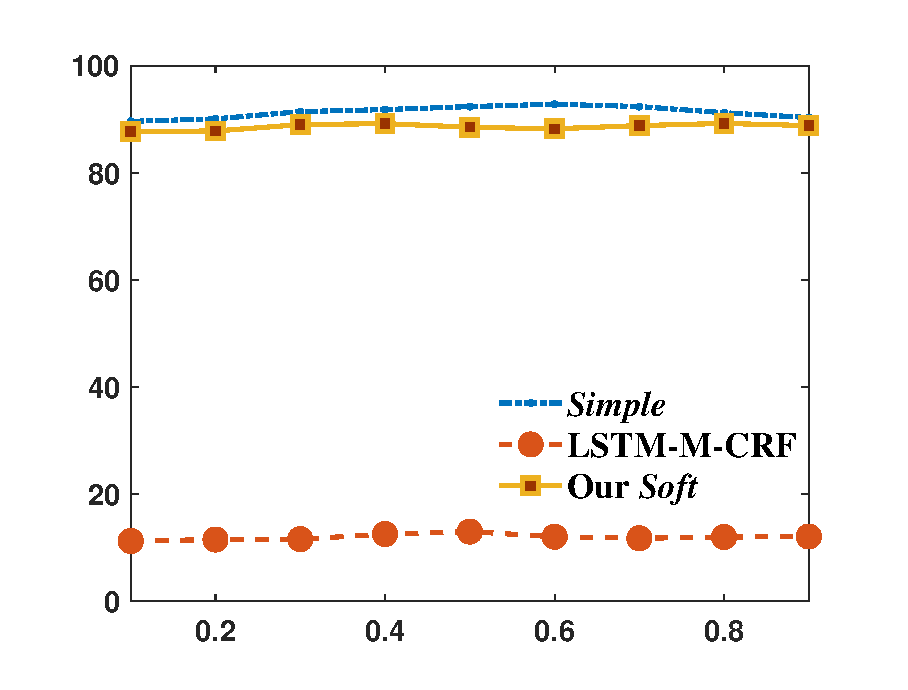
\includegraphics[width=2.4in]{Figures/conll2003precision.eps}
		%			\vspace{-5mm}
		\caption{Precision}
	\end{subfigure}
	\begin{subfigure}{0.45\linewidth}
		\centering
		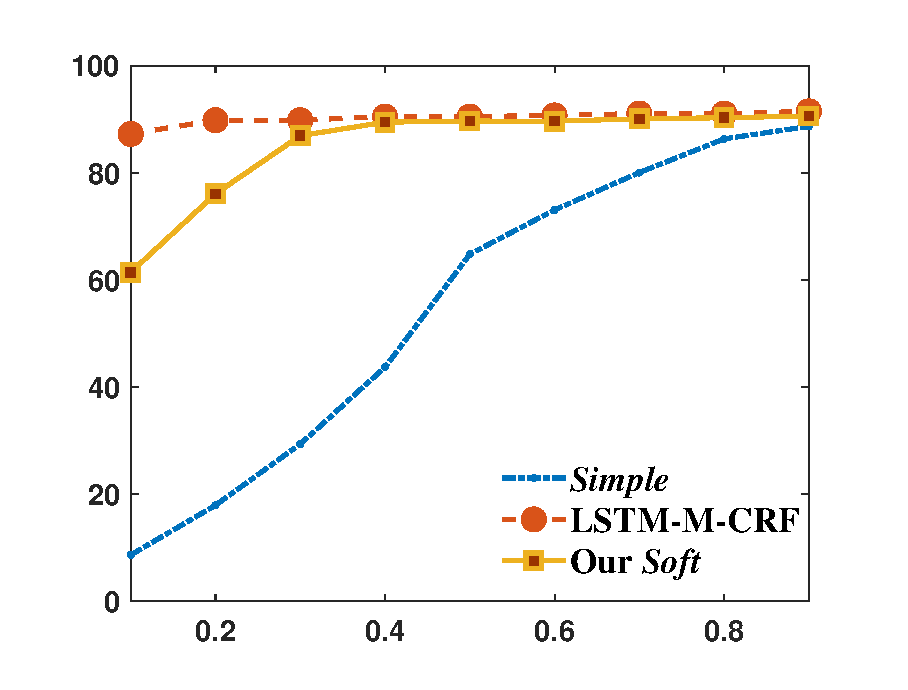
\includegraphics[width=2.4in]{Figures/conll2003recall.eps}
		%			\vspace{-5mm}
		\caption{Recall}
	\end{subfigure}
	\begin{subfigure}{0.45\linewidth}
		\centering
		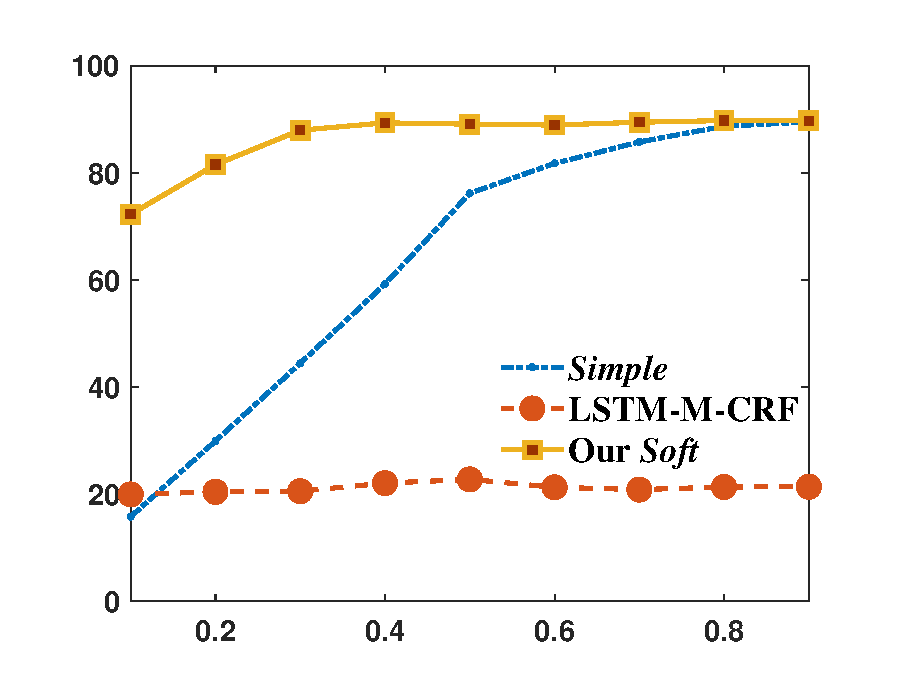
\includegraphics[width=2.4in]{Figures/conll2003.eps}
		%			\vspace{-5mm}
		\caption{$F$-score}
	\end{subfigure}
	%	}
	\caption{Precision, Recall and $F$-score with different $\rho$ on CoNLL-2003 dataset. }
	%	\vspace{-2mm}
	\label{fig:diffp}
\end{figure*}


%	\paragraph{Convergence Analysis}
%%\subsection{Convergence Analysis}
%We study the convergence of the $q$ distribution by evaluating the performance after each iterative training iteration. 
%Figure \ref{fig:cv} (left) shows the precision, recall and $F$-score performance of our {\it soft} variant on CoNLL-2003 dataset. 
%We can see the $F$-score keeps increasing and fluctuates at around 90 when the number of iteration is more than 3. 
%As expected, our approach performs similarly to the {\it Simple} baseline where the precision is high but recall is low. 
%The iterative process significantly improve the recall as well as the overall $F$-score until the $q$ distribution gradually converges. 
%In a sense, the iterative training process can retrieve many of the correct labels in training data. 
%
%
%With this definition, we can further calculate the recovery rate of correct labels in the training set recovered from the {\it soft} approach by counting the recovered labels. 
%
%\begin{figure}[t!]
%	\centering
%	\begin{subfigure}{0.5\columnwidth}
%		\centering
%		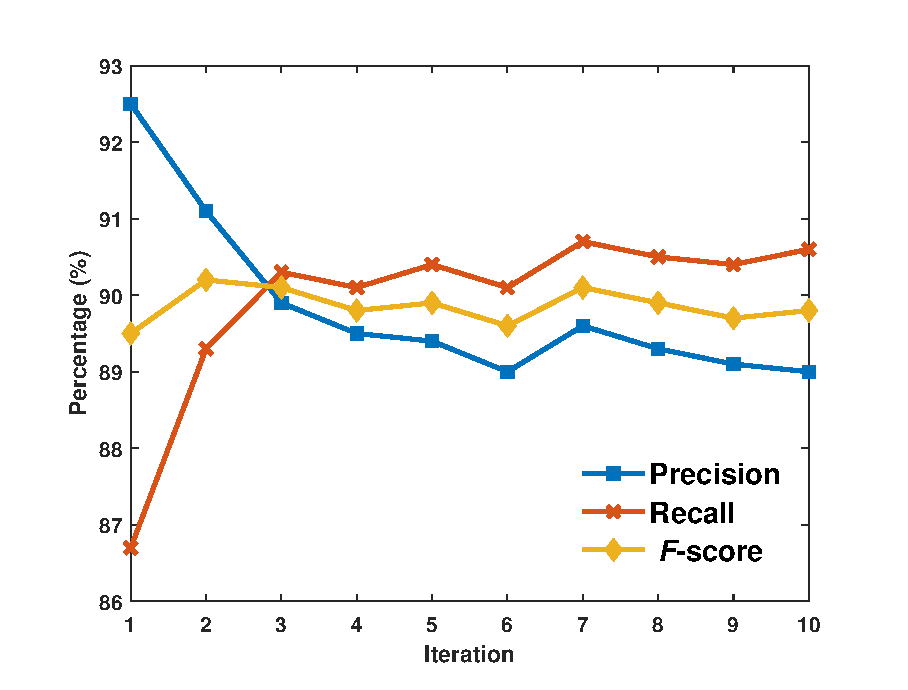
\includegraphics[width=1.4in]{imgs/cvperformance.eps}
%	\end{subfigure}
%	\begin{subfigure}{0.45\columnwidth}
%		\centering
%		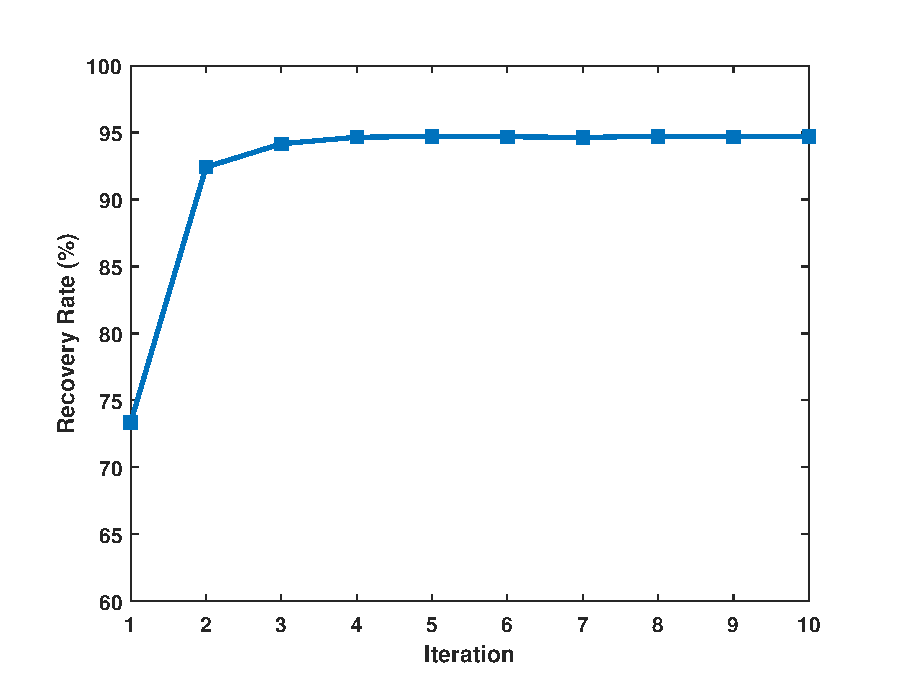
\includegraphics[width=1.4in]{imgs/conll2003recover.eps}
%	\end{subfigure}
%	\caption{Precision, recall and $F$-score performance (left) on CoNLL-2003 development set and the recovery rate (right) after each iteration.}
%	\label{fig:cv}
%\end{figure} 
%The expectation can be calculated efficiently using the forward-backward algorithm. 
%Figure \ref{fig:cv} (right) shows the recovery rate of the training set generated from our approaches. 
%The recovery rate is consistent with the finding of the convergence in $F$-score where it becomes stable at around 94\% after the $3^{rd}$ iteration. 
%The fast convergence of our approach is consistent with the observation by \citet{nivre2008integrating} where they did not observe significant improvement after the first few iterations. 

%	\begin{table}[t!]
%		\centering
%		\scalebox{0.7}{
%		\begin{tabular}{lcccc}
%			\toprule
%			& CoNLL-2003 & CoNLL-2002 & Taobao & Youku \\\midrule
%			\textsc{Err} (\%) & {\color{white}0}3.13 &{\color{white}0}7.79 & 11.06& {\color{white}0}7.00 \\
%%			 ~~{\small\it --is annotation err} & 29.81 &42.86 &72.17 &  60.67\\
%			\bottomrule
%		\end{tabular}
%		}
%		\caption{Percentage of errors {\color{red}(at entity level)??} that are made by our approaches  {\color{red}(soft??)} but are corrected by the {\it Complete} model.}
%		\label{tab:unavailable}
%	\end{table}

%	\paragraph{Effect of Unavailable Labels}
%	{\color{red}We further conduct analysis on how the unavailable labels keep the  model away from achieving high performance.
%	Table \ref{tab:unavailable} shows the error ratio of entities that are incorrectly predicted by our {\it soft} variant but correctly predicted by the {\it Complete} model. 
%	Our approach obtains small error rate against the {\it Complete} model on all datasets except Taobao. 
%	We found that there are many entities in the test set of Taobao appear in the training set and many of them are not annotated in our experiments. }


\section{Dependency-based Solution: As a Future Work}

Essentially, the problem mentioned above is the missing annotations of \textsc{o} labels (\textit{i.e.,} false negative). 
Observing the relationships between the named entities and dependency trees, we can somehow infer that some dependency relations also have strong correlations with the \textsc{o} labels.
On the other hand, if some candidate spans are not forming subtrees, it is very likely that the span is not an entity.

Using such relationships, we present a dependency-based solution which can efficiently solve the incomplete annotation problem rather than iterative training. 
The underlying solution is a future work for solving this problem.


\subsection{Entity Candidate Selection}
Given the properties we observed in Chapter \ref{Chapter3} and Chapter \ref{Chapter4}, we identify some entity candidates and non-entity words before actual training. 
Specifically, we can perform the following pre-processing and then train a marginal CRF~\cite{greenberg2018marginal} but in a semi-Markov manner. 
\begin{itemize}
	\item Obtain the dependency parse trees with existing dependency parser.
	\item As entities are very likely to form subtrees, for those spans that cannot form subtree, we eliminate those spans in a semi-Markov model. 
	\item On the other hand, we also focus on the dependency relations. If some word are associated with dependency relations (e.g., \textit{neg}) are not possible to be entities, we also eliminate them to be non-entity words.
\end{itemize}

After the elimination process is done, we have a constrained space of named entities. 
We can train the model by maximizing  the marginalized log-likelihood.


\section{Conclusions}
In this work, we identified several limitations associated with previous assumptions when performing sequence labeling with incomplete annotations, and focused on the named entity recognition task.
%	In this work, we identify several limitations associated with previous assumptions when performing NER with incomplete annotations.
We present a novel and easy-to-implement solution that works under a realistic and challenging assumption on the incomplete annotations.
Through extensive experiments and analysis, we demonstrate the effectiveness of our approach. 
Finally, we present a potential dependency-based solution as a future work. 

Although we focused on the task of named entity recognition in this work, we believe the proposed approach may find applications in some other  sequence labeling tasks or other more general structured prediction problems where the issue of incomplete annotations is involved.



% under this challenging assumption. 
%	On the other hand, we would like to apply our approach on multiple datasets from different domains as the underlying scenario is more common in practice. 

%	In the future, we would like to apply our approach to datasets from different domains as the underlying scenario is more common in practice. 
%In the future, we would like to apply our approach on multiple datasets from different domains as the underlying scenario is more common in practice. 


% Chapter Template

\chapter{Dependency-based Hybrid Trees for Semantic Parsing} % Main chapter title

\label{Chapter6} % Change X to a consecutive number; for referencing this chapter elsewhere, use \ref{ChapterX}

%----------------------------------------------------------------------------------------
%	SECTION 1
%----------------------------------------------------------------------------------------

\section{Introduction}
\label{sec:intro}

Semantic parsing is a fundamental task within the field of natural language processing (NLP).
Consider a natural language (NL) sentence and its corresponding meaning representation (MR) as illustrated in Figure \ref{fig:dhtexample}.
%Semantic parsing is the task of transforming the former to the latter  automatically.
Semantic parsing aims to transform the natural language sentences into machine interpretable meaning representations automatically. 
The task has been popular for decades and keeps receiving significant attention from the NLP community. 
Various systems~\cite{zelle1996learning,kate2005learning,zettlemoyer2005learning,liang11learning} were proposed over the years to deal with different types of semantic representations.
Such models include structure-based models~\cite{wong2006learning,lu2008generative,kwiatkowski2010inducing,jones2012semantic}  and neural network based models~\cite{dong2016language,cheng2017learning}. 


\begin{figure}[h!]
	\centering
	\scalebox{1}{
		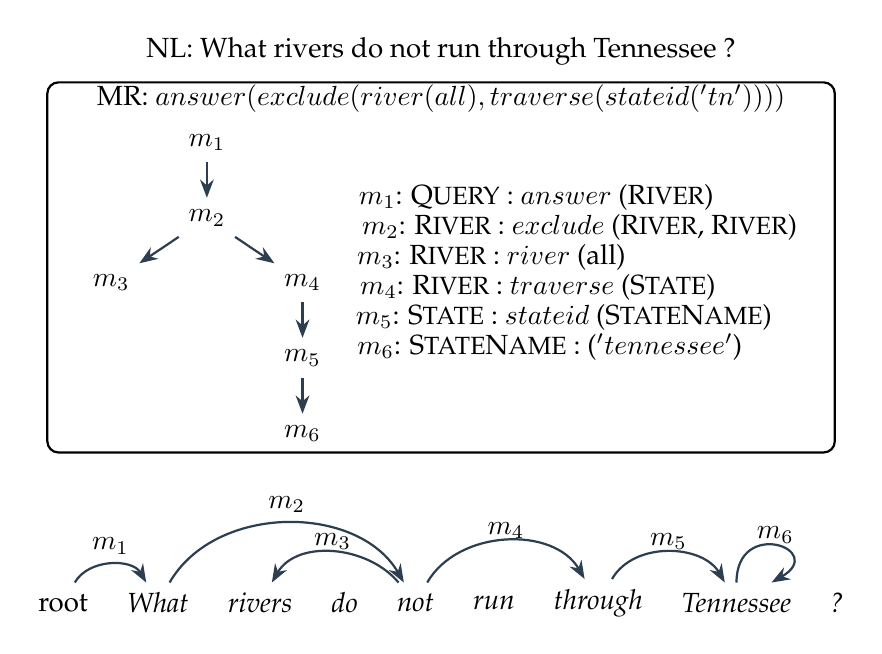
\begin{tikzpicture}[node distance=2.0mm and 2.5mm, >=Stealth, 
		semantic/.style={draw=none, minimum height=5mm, rectangle},
		word/.style={draw=none, minimum height=5mm, rectangle},
		olabel/.style={draw=none, circle, minimum height=9mm, minimum width=9mm,line width=1pt, inner sep=2pt, fill=lowblue, text=fontgray, label={center:\textsc{o}}},
		bperlabel/.style={draw=none, circle, minimum height=9mm, minimum width=9mm,line width=1pt, inner sep=2pt, fill=lowblue, text=black, label={center:\textsc{per}}},
		borglabel/.style={draw=none, circle, minimum height=9mm, minimum width=9mm,line width=1pt, inner sep=2pt, fill=lowblue, text=black, label={center:\textsc{org}}},
		bgpelabel/.style={draw=none, circle, minimum height=9mm, minimum width=9mm,line width=1pt, inner sep=2pt, fill=lowblue, text=black, label={center:\textsc{Misc}}},
		nnlabel/.style={draw=none, circle, minimum height=9mm, minimum width=9mm,line width=1pt, inner sep=2pt, fill=mypumpkin, text=black, label={center:\textsc{Gpe}}},
		invis/.style={draw=none, circle, minimum height=9mm, minimum width=9mm,line width=1pt, inner sep=2pt, fill=none, text=fontgray},
		chainLine/.style={line width=1pt,-, color=fontgray}	%		,background rectangle/.style={fill=olive!45}, show background rectangle
		]
		
		\node[semantic](s1) [] {NL: What rivers do not run through Tennessee ?};
		\node[semantic](mr1) [below= of s1, yshift=2mm] {MR: $answer(exclude(river(all), traverse(stateid('tn'))))$}; 
		\node[draw=black, minimum height=47mm, minimum width=100mm, rectangle, line width=0.8pt, rounded corners] (box) [yshift=-27.5mm] {};
		
		\node[word](m1) [below left = of s1, yshift = -4mm, xshift=15mm] {$m_1$};
		\node[word](m2) [below=of m1, yshift=-2.5mm] {$m_2$};
		\node[word](m3) [below left=of m2, yshift=-1mm,xshift=-2.5mm] {$m_3$};
		\node[word](m4) [below right=of m2, yshift=-1mm, xshift=2.5mm] {$m_4$};
		\node[word](m5) [below =of m4, yshift=-2.5mm] {$m_5$};
		\node[word](m6) [below =of m5, yshift=-2.5mm] {$m_6$};
		
		\node[word](m1r)[right= of m1, xshift=12mm, yshift=-7mm] {$m_1$: Q{\small{UERY}} : $answer$ (R{\small{IVER}})};
		\node[word](m2r)[below= of m1r, yshift=4mm, xshift=5.5mm] {$m_2$: R{\small{IVER}} : $exclude$ (R{\small{IVER}}, R{\small{IVER}})};
		\node[word](m3r)[below= of m2r, yshift=4mm, xshift=-11.2mm] {$m_3$: R{\small{IVER}} : $river$ (all)};
		\node[word](m4r)[below= of m3r, yshift=4mm, xshift=5.9mm] {$m_4$: R{\small{IVER}} : $traverse$ (S{\small{TATE}})};
		\node[word](m5r)[below= of m4r, yshift=4mm, xshift=3.3mm] {$m_5$: S{\small{TATE}} : $stateid$ (S{\small{TATE}}N{\small{AME}})};
		\node[word](m6r)[below= of m5r, yshift=4mm, xshift=-1.8mm] {$m_6$: S{\small{TATE}}N{\small{AME}} : ($'tennessee'$)};
		
		\draw [line width=0.8pt,->, color=fontgray]  (m1) to [] node[]{} (m2);
		\draw [line width=0.8pt,->, color=fontgray]  (m2) to [] node[]{} (m3);
		\draw [line width=0.8pt,->, color=fontgray]  (m2) to [] node[]{} (m4);
		\draw [line width=0.8pt,->, color=fontgray]  (m4) to [] node[]{} (m5);
		\draw [line width=0.8pt,->, color=fontgray]  (m5) to [] node[]{} (m6);
		
		%		\Tree [.\node(root){$m_1$: Q{\small{UERY}} : $answer$ (R{\small{IVER}})}; [.{$m_2$: R{\small{IVER}}: $exclude$ (R{\small{IVER}}, R{\small{IVER}})} {$m_3 \equiv$ R{\small{IVER}} : $state$ (all)} [.{$m_4 \equiv$ R{\small{IVER}} : $traverse$ (S{\small{TATE}})} [.{$m_5 \equiv $S{\small{TATE}} : $stateid$ (S{\small{TATE}}N{\small{AME}})} {$m_6 \equiv$  S{\small{TATE}}N{\small{AME}} : ($'tennessee'$)} ]] ]]
		
		\node[word](w0) [below = of s1, xshift = -48mm, yshift=-62.5mm] {root};
		\node[word](w1) [right = of w0] {{\em What}};
		\node[invis](rootop) [above = of w0, yshift=8mm] {};
		\node[word](w2) [right = of w1] {{\em rivers}};
		\node[word](w3) [right = of w2] {{\em do}};
		\node[word](w4) [right = of w3] {{\em not}};
		\node[word](w5) [right = of w4] {{\em run}};
		\node[word](w6) [right = of w5] {{\em through}};
		\node[word](w7) [right = of w6] {{\em Tennessee}};
		\node[word](w8) [right = of w7] {{\em ?}};
		
		\draw [line width=0.8pt,->, color=fontgray]  (w0) to [out=60,in=120, looseness=1] node[above, yshift=0mm, color=black]{$m_1$} (w1);
		\draw [line width=0.8pt,->, color=fontgray]  (w1) to [out=60,in=120, looseness=1] node[above, color=black]{$m_2$} (w4);
		\draw [line width=0.8pt,->, color=fontgray]  (w4) to [out=130,in=60, looseness=1] node[above, yshift=-1mm, color=black]{$m_3$} (w2);
		\draw [line width=0.8pt,->, color=fontgray]  (w4) to [out=60,in=120, looseness=1] node[above, yshift=-1mm, color=black]{$m_4$} (w6);
		\draw [line width=0.8pt,->, color=fontgray]  (w6) to [out=60,in=120, looseness=1] node[above, yshift=-1mm, color=black]{$m_5$} (w7);
		\draw [line width=0.8pt,->, color=fontgray]  (w7) to [out=90,in=30, looseness=4.8] node[above, yshift=-1mm, color=black]{$m_6$} (w7);
		%		\draw[line width=0.8pt,->, color=fontgray] (w6.0) arc (90:180+264:4mm);
		%		\node[semantic](s2) [below= of w4] {{\em What} ({\em not} ({\em rivers}, ({\em through} ({\em Tennessee}))))};
		\end{tikzpicture} 
	}
	%	\vspace{-2mm}
	\caption{Top: natural language (NL) sentence; middle: meaning representation (MR); bottom:  dependency-based hybrid tree representation.}
	%	\vspace{1mm}
	%	\vspace{-5mm}
	\label{fig:dhtexample}
\end{figure}

Following various previous research efforts \cite{wong2006learning,lu2008generative,jones2012semantic},  in this work, we adopt a popular class of semantic formalism -- logical forms that can be equivalently represented as tree structures.
The  tree representation of an example MR is shown in the middle of Figure \ref{fig:example}.
One challenge associated with building a semantic parser is that the exact correspondence between the words and atomic semantic units are not explicitly given during the training phase.
The key to the building of a successful semantic parsing model lies in the identification of a good {\em joint} latent representation of both the sentence and its corresponding semantics.
Example joint representations proposed in the literature include a chart used in phrase-based translation \cite{wong2006learning}, a constituency tree-like representation known as {\em hybrid tree} \cite{lu2008generative}, and a CCG-based derivation tree \cite{kwiatkowski2010inducing}.

Previous research efforts have shown the effectiveness of using dependency structures to extract semantic representations~\cite{debusmann2004relational,cimiano2009flexible,bedaride2011deep,stanovsky2016getting}. 
Recently, \citet{reddy2016transforming,reddy2017universal} proposed a model to construct logical representations from sentences that are parsed into dependency structures.
Their work demonstrates the connection between the dependency structures of a sentence and its underlying semantics.
Although their setup and objectives are different from ours where externally trained dependency parsers are assumed available and their system was trained to use the semantics for a specific down-stream task, the success of their work motivates us to propose a novel joint  representation that can explicitly capture dependency structures among words for the semantic parsing task.

%Various semantic formalisms have been used in semantic parsing: tree-structured semantic representations~\cite{kate2006using,wong2006learning}, the lambda-calculus logical form~\cite{zettlemoyer2005learning,wong2007learning} and dependency-based semantic representations (DCS)~\cite{liang2013learning}. 
%Consider the meaning representation in the form of tree structure shown in Figure \ref{fig:example}.
%In this work, we adopt the variable-free semantic representations where the underlying meaning representations (MR) can be expressed in the form of tree structures. 
%An example tree-structured meaning representation taken from the GeoQuery dataset is shown at the top of Figure \ref{fig:example}. 
%Each tree node in the semantic tree represents an atomic semantic unit $m_i$. 
%As shown in the middle of Figure \ref{fig:example}, the trees corresponds to the natural language (NL) sentences can be further represented as a string-form meaning representation (MR) via function composition. 
%We present more details of tree-structured semantic representation in Section \ref{sec:semantics}. 



%Figure \ref{fig:example} shows an example of such a tree-structured 
%Such semantics can be represented by tree structure as shown in Figure \ref{fig:example}. 
%Each node in the tree is an atomic semantic unit referred as $m$ for short. 
%More details of the tree-structured semantic representations are given in Section \ref{sec:semantics}. 


%Learning such tree-structured semantic representations is typically more challenging as the complete semantic trees are not explicitly associated (or aligned) to the natural language sentences. 
%In order to capture the interactions between the semantics and natural language sentences, we observe that the semantic units are actually related to some of the natural language words and can represent the directed relationship between the words. 
%As shown at the bottom of Figure \ref{fig:example}, we can jointly represent the semantic representation and the natural language sentence into a dependency tree where the semantic units are interpreted as the dependency (or relationship) between two words\footnote{We introduce a special token ``{\em root}'' to represent the root of a dependency tree.}. 
%We call the resulting joint representation {\em dependency-based hybrid tree} (\textsc{DepHT}).
%For example, $m_2$ (i.e., R{\small{IVER}}: $exclude$ (R{\small{IVER}}, R{\small{IVER}})) is the relation of the dependency from the parent ``{\em What}'' to the child ``{\em not}''. 
%On the other hand, the words (i.e., ``{\em What rivers do not}'') that covered by this dependency arc also explicitly express the semantic unit $m_2$. 
%Such {\em parent-child dependency} and {\em span-level semantic information} are highly meaningful to connect the underlying semantic representation and the natural language sentences. 
%The {\em span-level semantic information} was shown to be effective in the semantic parsing task~\cite{kwiatkowski2010inducing,liang2013learning,lu2014semantic,susanto2017semantic}. 

%Additionally, with the representation of {\em dependency-based hybrid tree}, we can perceive how the underlying semantics express and change upon the natural language words by following the dependency tree. 
%Specifically, we can further extract a variable-free logical representation using natural language words from the {\em dependency-based hybrid tree} in Figure \ref{fig:example}:
%\begin{figure}[h!]
%	\centering
%	\scalebox{0.8}{
%		\begin{tikzpicture}[node distance=2.0mm and 2.5mm, >=Stealth, 
%		semantic/.style={draw=none, minimum height=5mm, rectangle},
%		]
%		\node[semantic](s1) [] {{\em What} ({\em not} ({\em rivers}, ({\em through} ({\em Tennessee}))))};
%		\node[semantic](mr1) [below= of s1, yshift=3mm] {MR: $answer(exclude(river(all), traverse(stateid('tn'))))$}; 
%		\end{tikzpicture} 
%	}
%	\vspace*{-7mm}
%\end{figure}

%\noindent We can see that the extracted variable-free logical expression from the words is similar to the meaning representation in a sense that the functional words have similar meanings, which makes our {\em dependency-based hybrid tree} have a decent interpretability on the meaning representation. 
%%the advantage of interpreting the meaning representation.   
%
%As such useful dependencies are not given in semantic parsing tasks, we model them as latent variables and the semantics are the latent dependencies between the natural language words. 
%Note that our task is different from semantic dependency parsing~\cite{oepen2015semeval} SemEval shared task, which is the task of recovering predicate-argument relationships and related to semantic role labeling. 


%We propose a novel {\em dependency-based hybrid tree} representation, a new joint latent structured representation of both semantics and natural language sentences. 
%Most of previous work~\cite{liang11learning,dong2016language,cheng2017learning,susanto2017neural} model the semantic representations without explicitly capturing the interactions between the semantics and natural language words, which potentially makes the system/model less interpretable. 
%\citet{lu2014semantic} proposed a \textit{relaxed hybrid tree} model which capture span-level interactions between the semantic units and natural language words as well as the long-distance dependencies. 
%\citet{reddy2016transforming} deterministically transforms the syntactic dependencies into logical forms and the results depend on the quality from dependency parsing. 
%Inspired by both literatures, we propose a novel latent semantic representations involved the natural language words as shown in the bottom of Figure \ref{fig:example}. 
%The semantics are modeled as latent dependency trees over natural language words. 
%We believe such representations capture span-level interactions as in \cite{lu2014semantic} and we do not require external syntactic dependency parsers to build semantic representations as in \cite{reddy2016transforming}. 
%For example, ``\textit{What rivers do not}'' is covered by the arc from ``\textit{What}'' to ``\textit{not}'' and corresponding semantic unit is  $m_2$ (i.e., R{\small{IVER}}: $exclude$ (R{\small{IVER}}, R{\small{IVER}})). 
%Such information is similarly captured in hybrid tree model and the semantic information can be captured by dependencies between specific words. 
%Furthermore, it is clear to interpret the semantics following the dependency tree along the natural language words and semantic units. 
In this work, we propose a new joint representation for both semantics and words, presenting a new model for semantic parsing. 
Our main contributions can be summarized as follows: 
\begin{itemize}

\item We present a novel {\em dependency-based hybrid tree} representation that captures both words and semantics in a joint manner.
Such a dependency tree reveals semantic dependencies between words which are easily interpretable. 

%	\item We build a semantic parser with such a representation, presenting 
\item We show that exact dynamic programming algorithms for inference can be designed on top of our new representation.  We further show that the model can be integrated with neural networks for improved effectiveness.
%	propose a neural graphical model to learn the latent {\em dependency-based hybrid tree} structure. 
%		Our efficient dynamic-programming algorithm allows the model to perform tractable inference over the graphical model and the neural networks. 
\item Extensive experiments conducted on the standard multilingual GeoQuery dataset 
%	with eight languages
show that our model outperforms the state-of-the-art models on 7 out of 8 languages. Further analysis confirms the effectiveness of our  dependency-based representation.
\end{itemize}

To the best of our knowledge, this is the first work that models the semantics as latent dependencies between   words for semantic parsing. 

{\color{red}
	
}



\section{Related Work}
The literature on semantic parsing has focused on various types of semantic formalisms. 
The $\lambda$-calculus expressions~\cite{zettlemoyer2005learning} have been popular and widely used in semantic parsing tasks over recent years~\cite{dong2016language,gardner2017open,reddy2016transforming,reddy2017universal,susanto2017neural,cheng2017learning}. 
Dependency-based compositional semantics (DCS)\footnote{Unlike ours, their work captures dependencies between  semantic units but not natural language words.} was introduced by \citet{liang11learning}, whose extension, $\lambda$-DCS, was later proposed by \citet{liang2013lambda}. 
Various models~\cite{berant2013semantic,wang2015building,jia-liang:2016:P16-1}  on semantic parsing with the $\lambda$-DCS formalism were proposed. 
In this work, we focus on the tree-structured semantic formalism which has been examined by various research efforts~\cite{wong2006learning,kate2006using,lu2008generative,kwiatkowski2010inducing,jones2012semantic,lu2014semantic,yan2018learn}.

\citet{wong2006learning} proposed the \textsc{Wasp} semantic parser 
that regards the task as a phrase-based machine translation problem.
%using statistical phrase-based machine translation approach by regarding the mapping natural language words to semantic representations as an alignment problem. 
\citet{lu2008generative} proposed a generative process to generate natural language words and semantic units in a joint model. 
The resulting representation is called \textit{hybrid tree} where both natural language words and semantics are encoded into a joint representation. 
The \textsc{UBL}-s~\cite{kwiatkowski2010inducing} parser applied the CCG grammar~\cite{steedman1996surface} to model the joint representation of both semantic units and contiguous word sequences which do not overlap with one another. 
\citet{jones2012semantic} applied a generative process with Bayesian tree transducer and their model also simultaneously generates the meaning representations and natural language words. 
\citet{lu2014semantic,lu2015constrained} proposed a discriminative version of the hybrid tree model of \cite{lu2008generative} where richer features can be captured. 
\citet{dong2016language} proposed a sequence-to-tree model using recurrent neural networks where the decoder can branch out to produce tree structures. 
\citet{susanto2017semantic} augmented the discriminative {hybrid tree} model with multilayer perceptron and achieved state-of-the-art performance. 




There exists another line of work that applies given syntactic dependency information to semantic parsing. 
\citet{titov2011bayesian} decomposed a syntactic dependency tree into fragments and modeled the semantics as relations between the fragments. 
\citet{poon2013grounded} learned to derive semantic structures based on syntactic dependency trees predicted by the Stanford dependency parser.
%modeled the semantic units on syntactic dependency-tree nodes and edges.
\citet{reddy2016transforming,reddy2017universal} proposed a linguistically motivated procedure to transform syntactic dependencies into logical forms. 
Their semantic parsing performance relies on the quality of the syntactic dependencies.
Unlike such efforts, we do not require external syntactic dependencies, but model the semantic units as latent dependencies between natural language words. 

\section{Approach}

%OK

%We briefly describe the variable-free semantics and introduce our {\em dependency-based hybrid tree} model in this section. 
%We further present a dynamic-programing algorithm to allow tractable inference during training and decoding. 

\subsection{Variable-free Semantics}
\label{sec:semantics}
The variable-free semantic representations in the form of FunQL~\cite{kate2005learning} used by the de-facto GeoQuery dataset~\cite{zelle1996learning} encode semantic compositionality of the logical forms~\cite{cheng2017learning}. 
In the tree-structured semantic representations as illustrated in Figure \ref{fig:example}, each tree node is a semantic unit of the following form:
\begin{equation*}
m_i \equiv \tau_\alpha : p_\alpha(\tau_\beta ^ *)
\end{equation*}
%\begin{center}
%	\begin{tabular}{c}
%		$
%		m_i \equiv \tau_\alpha : p_\alpha(\tau_\beta ^ *)
%		$
%	\end{tabular}
%\end{center}
where $m_i$ denotes the complete semantic unit, which consists of semantic type $\tau_\alpha$, function symbol $p_\alpha$ and an argument list of semantic types $\tau_\beta^*$ (here $*$ denotes that there can be 0, 1, or 2 semantic types in the  argument list. This number is known as the {\em arity} of $m_i$). 
Each semantic unit can be regarded as a function that takes in other (partial) semantic representations of certain types as arguments and returns a semantic representation of a specific type.
For example in Figure \ref{fig:example}, the root unit is represented by $m_1$, the type of this unit is \textsc{Query}, the function name is $answer$ and it has a single argument  \textsc{River} which is a semantic type. 
With  recursive function composition, we can obtain a complete MR as shown in Figure \ref{fig:example}.
%In our dependency-based representation, each semantic unit serves as the dependency label between the natural language words as shown at the bottom of Figure \ref{fig:example}. 

\subsection{Dependency-based Hybrid Trees}
To jointly encode the tree-structured semantics $\boldsymbol{m}$ and a natural language sentence $\boldsymbol{n}$, we introduce our novel {\em dependency-based hybrid tree}. 
Figure \ref{fig:dhtexample} (right) shows the two equivalent ways of visualizing the {dependency-based hybrid tree} based on the example given in Figure \ref{fig:example}. 
In this example, the bold symbol $\boldsymbol{m}$ is the tree-structured semantics $m_1 (m_2 (m_3, m_4(m_5(m_6))))$ and $\boldsymbol{n}$ is the sentence $\{w_1, w_2, \cdots,w_8\}$\footnote{We also introduce a special token ``{\em root}'' as $w_0$.}. 
Our {dependency-based hybrid tree} $\boldsymbol{t}$ consists of a set of dependencies  between the natural language words, each of which is labeled with a semantic unit. 
Formally, a dependency arc is represented as $(w_p, w_c, m_i)$, where $w_p$ is the {\em parent} of this dependency, $w_c$ is the {\em child}, and $m_i$ is the semantic unit that serves as the {\em label} for the dependency arc. 
A valid dependency-based hybrid tree (with respect to a given semantic representation) allows one to recover the correct semantics from it.
Thus, one constraint is that for any two adjacent dependencies $(w_p, w_c, m_i)$ and $(w_p^\prime, w_c^\prime, m_j)$, where $w_c \equiv w_p^\prime$, $m_i$ must be the parent of $m_j$ in the tree-structured representation $\boldsymbol{m}$.  
For example, in Figure \ref{fig:dhtexample}, the dependencies ({\em not}, {\em through}, $m_4$) and ({\em through}, {\em Tennessee}, $m_5$) satisfy the above condition. 
However, we cannot replace ({\em through}, {\em Tennessee}, $m_5$) with, for example, ({\em through}, {\em Tennessee}, $m_6$), since $m_6$ is not the child of $m_4$. 
Furthermore, the number of children for a word in the dependency tree should be consistent with the arity of the corresponding semantic unit that points to it. 
For example, ``{\em not}'' has 2 children in our {dependency-based hybrid tree} representation because the semantic unit $m_2$ (i.e., R{\small{IVER}} : $exclude$ (R{\small{IVER}}, R{\small{IVER}})) has arity 2. 
Also, ``{\em rivers}'' is the leaf as $m_3$, which points to it, has arity 0.
We will discuss in Section \ref{sec:patterns} on how to derive the set of allowable dependency-based hybrid trees for a given $(\boldsymbol{m},\boldsymbol{n})$ pair.
% and has no child.
%no semantic unit argument.





To understand the potential advantages of our new joint representation, we compare it with the {\em relaxed hybrid tree} representation~\cite{lu2014semantic}, which is illustrated on the left of Figure \ref{fig:dhtexample}.
We highlight some similarities and differences between the two representations from the {\em span level} and {\em word level} perspectives.

\begin{figure*}[h!]
	\centering
	\scalebox{0.75}{
		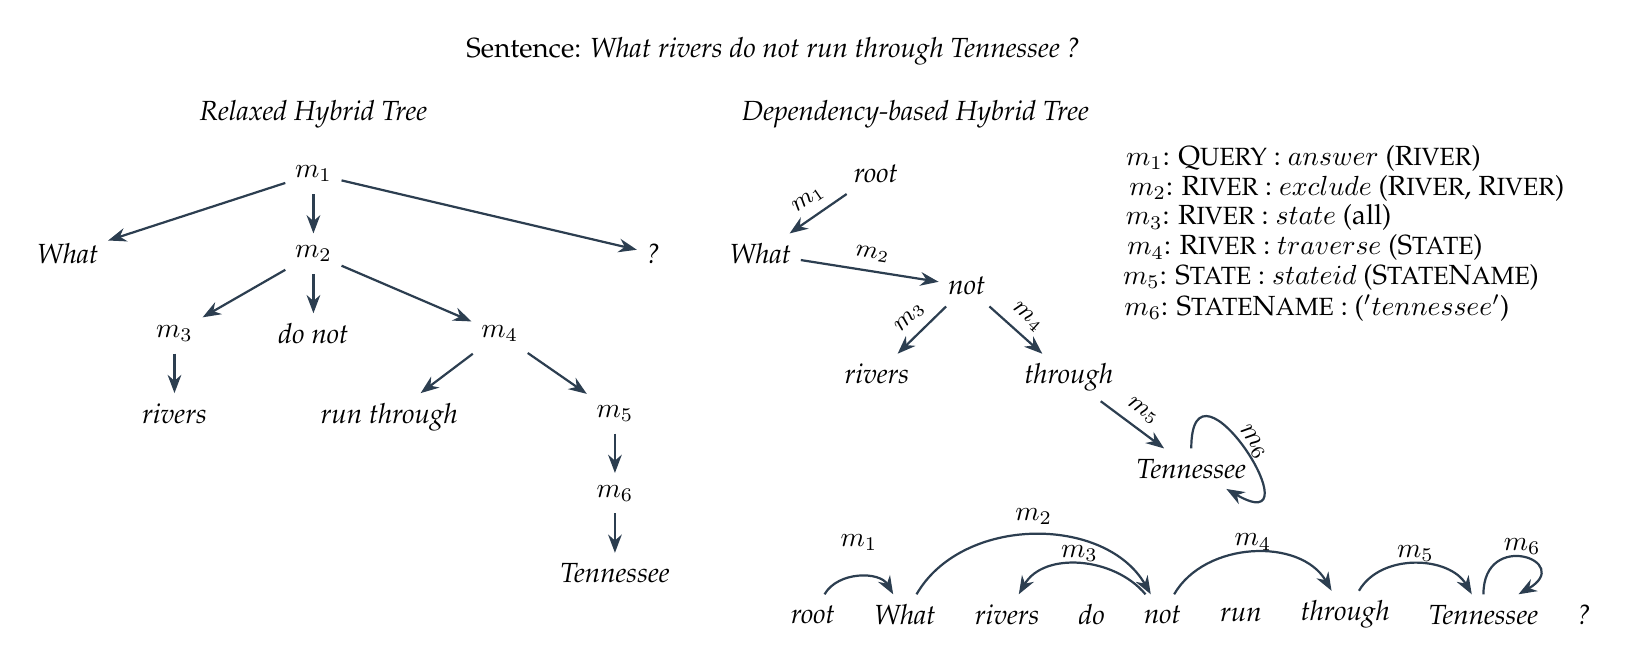
\begin{tikzpicture}[node distance=2.0mm and 2.5mm, >=Stealth, 
		semantic/.style={draw=none, minimum height=5mm, rectangle},
		word/.style={draw=none, minimum height=5mm, rectangle},
		olabel/.style={draw=none, circle, minimum height=9mm, minimum width=9mm,line width=1pt, inner sep=2pt, fill=lowblue, text=fontgray, label={center:\textsc{o}}},
		bperlabel/.style={draw=none, circle, minimum height=9mm, minimum width=9mm,line width=1pt, inner sep=2pt, fill=lowblue, text=black, label={center:\textsc{per}}},
		borglabel/.style={draw=none, circle, minimum height=9mm, minimum width=9mm,line width=1pt, inner sep=2pt, fill=lowblue, text=black, label={center:\textsc{org}}},
		bgpelabel/.style={draw=none, circle, minimum height=9mm, minimum width=9mm,line width=1pt, inner sep=2pt, fill=lowblue, text=black, label={center:\textsc{Misc}}},
		nnlabel/.style={draw=none, circle, minimum height=9mm, minimum width=9mm,line width=1pt, inner sep=2pt, fill=mypumpkin, text=black, label={center:\textsc{Gpe}}},
		invis/.style={draw=none, circle, minimum height=9mm, minimum width=9mm,line width=1pt, inner sep=2pt, fill=none, text=fontgray},
		chainLine/.style={line width=0.8pt,->, color=fontgray}	%		,background rectangle/.style={fill=olive!45}, show background rectangle
		]
		\node[semantic](sent) [] {Sentence: {\em What rivers do not run through Tennessee ?}}; 
		
		\node[word](htname) [below left = of sent, xshift=0mm] {{\em Relaxed Hybrid Tree}};
		
		\node[word](hm1) [below = of htname, xshift=0mm] {$m_1$};
		\node[word](hw1) [below left = of hm1, xshift=-20mm, yshift=-3mm] {{\em What}};
		\node[word](hw8) [below right = of hm1, xshift=35mm, yshift=-3mm] {{\em ?}};
		\node[word](hm2) [below = of hm1, xshift=0mm, yshift=-3mm] {$m_2$};
		
		\node[word](hm3) [below left= of hm2, xshift=-8mm, yshift=-3mm] {$m_3$};
		\node[word](hm4) [below right= of hm2, xshift=14mm, yshift=-3mm] {$m_4$};
		\node[word](hw34) [below= of hm2, xshift=0mm, yshift=-3mm] {{\em do not}};
		
		\node[word](hw2) [below= of hm3, xshift=0mm, yshift=-3mm] {{\em rivers}};
		
		\node[word](hm5) [below right= of hm4, xshift=5mm, yshift=-3mm] {$m_5$};
		\node[word](hw56) [below left= of hm4, xshift=2mm, yshift=-3mm] {{\em run through}};
		\node[word](hm6) [below= of hm5, xshift=0mm, yshift=-3mm] {$m_6$};
		\node[word](hw7) [below= of hm6, xshift=0mm, yshift=-3mm] {{\em Tennessee}};
		
		\draw [chainLine] (hm1) to [] node[] {} (hw1);
		\draw [chainLine] (hm1) to [] node[] {} (hm2);
		\draw [chainLine] (hm1) to [] node[] {} (hw8);
		
		\draw [chainLine] (hm2) to [] node[] {} (hm3);
		\draw [chainLine] (hm2) to [] node[] {} (hw34);
		\draw [chainLine] (hm2) to [] node[] {} (hm4);
		
		\draw [chainLine] (hm3) to [] node[] {} (hw2);
		\draw [chainLine] (hm4) to [] node[] {} (hw56);
		\draw [chainLine] (hm4) to [] node[] {} (hm5);
		
		\draw [chainLine] (hm5) to [] node[] {} (hm6);
		\draw [chainLine] (hm6) to [] node[] {} (hw7);
		
		
		\node[word](dhtname) [below right = of sent, xshift=-48mm] {{\em Dependency-based Hybrid Tree}};
		\node[word](root) [below = of dhtname, xshift=-5mm] {\textit{root}};
		\node[word](what) [below left = of root, yshift=-3mm, xshift=-3mm] {\textit{What}};
		%		\node[invis](rootop) [above = of w0, yshift=8mm] {};
		\node[word](not) [below right = of what, xshift=15mm, yshift=3mm] {\textit{not}};
		\node[word](rivers) [below left = of not, yshift=-4mm] {\textit{rivers}};
		\node[word](through) [below right = of not, yshift=-4mm] {\textit{through}};
		\node[word](tennessee) [below right = of through, yshift=-4mm, xshift=-2mm] {\textit{Tennessee}};
		
		\node[word](m1)[right= of root, xshift=24mm, yshift=2mm] {$m_1$: Q{\small{UERY}} : $answer$ (R{\small{IVER}})};
		\node[word](m2)[below= of m1, yshift=4mm, xshift=5.5mm] {$m_2$: R{\small{IVER}} : $exclude$ (R{\small{IVER}}, R{\small{IVER}})};
		\node[word](m3)[below= of m2, yshift=4mm, xshift=-11.2mm] {$m_3$: R{\small{IVER}} : $state$ (all)};
		\node[word](m4)[below= of m3, yshift=4mm, xshift=5.9mm] {$m_4$: R{\small{IVER}} : $traverse$ (S{\small{TATE}})};
		\node[word](m5)[below= of m4, yshift=4mm, xshift=3.3mm] {$m_5$: S{\small{TATE}} : $stateid$ (S{\small{TATE}}N{\small{AME}})};
		\node[word](m6)[below= of m5, yshift=4mm, xshift=-1.8mm] {$m_6$: S{\small{TATE}}N{\small{AME}} : ($'tennessee'$)};
		
		%		\Tree [.\node(root){$m_1 \equiv $ Q{\small{UERY}} : $answer$ (R{\small{IVER}})}; [.{$m_2 \equiv $ R{\small{IVER}}: $exclude$ (R{\small{IVER}}, R{\small{IVER}})} {$m_3 \equiv$ R{\small{IVER}} : $state$ (all)} [.{$m_4 \equiv$ R{\small{IVER}} : $traverse$ (S{\small{TATE}})} [.{$m_5 \equiv $S{\small{TATE}} : $stateid$ (S{\small{TATE}}N{\small{AME}})} {$m_6 \equiv$  S{\small{TATE}}N{\small{AME}} : ($'texas'$)} ]] ]]
		
		\draw [chainLine] (root) to [] node[above, color=black,sloped] {\small  $m_1$} (what);
		\draw [chainLine] (what) to [] node[above, color=black,sloped] {\small  $m_2$} (not);
		\draw [chainLine] (not) to [] node[above, color=black,sloped] {\small  $m_3$} (rivers);
		\draw [chainLine] (not) to [] node[above, color=black,sloped] {\small  $m_4$} (through);
		\draw [chainLine] (through) to [] node[above, color=black,sloped] {\small  $m_5$} (tennessee);
		\draw [line width=0.8pt,->, color=fontgray]  (tennessee) to [out=90,in=-30, looseness=5.2] node[above, yshift=-1mm, color=black, sloped]{$m_6$} (tennessee);
		
		\node[word](wroot) [below = of sent, xshift = 5mm, yshift=-64mm] {{\em root}};
		\node[word](w0) [right = of wroot] {{\em What}};
		%		\node[invis](rootop) [above = of w0, yshift=8mm] {};
		\node[word](w1) [right = of w0] {{\em rivers}};
		\node[word](w2) [right = of w1] {{\em do}};
		\node[word](w3) [right = of w2] {{\em not}};
		\node[word](w4) [right = of w3] {{\em run}};
		\node[word](w5) [right = of w4] {{\em through}};
		\node[word](w6) [right = of w5] {{\em Tennessee}};
		\node[word](w7) [right = of w6] {{\em ?}};
		
		\draw [line width=0.8pt,->, color=fontgray]  (wroot) to [out=60,in=120, looseness=1] node[above, yshift=2mm, color=black]{$m_1$} (w0);
		\draw [line width=0.8pt,->, color=fontgray]  (w0) to [out=60,in=120, looseness=1] node[above, color=black]{$m_2$} (w3);
		\draw [line width=0.8pt,->, color=fontgray]  (w3) to [out=130,in=60, looseness=1] node[above, yshift=-1mm, color=black]{$m_3$} (w1);
		\draw [line width=0.8pt,->, color=fontgray]  (w3) to [out=60,in=120, looseness=1] node[above, yshift=-1mm, color=black]{$m_4$} (w5);
		\draw [line width=0.8pt,->, color=fontgray]  (w5) to [out=60,in=120, looseness=1] node[above, yshift=-1mm, color=black]{$m_5$} (w6);
		\draw [line width=0.8pt,->, color=fontgray]  (w6) to [out=90,in=30, looseness=4.8] node[above, yshift=-1mm, color=black]{$m_6$} (w6);
		\end{tikzpicture} 
	}
	%	\vspace*{-3mm}
	\caption{The \textit{relaxed hybrid tree} (left)~\cite{lu2014semantic} and our {\em dependency-based hybrid tree} (right) as well as the flat representation (bottom right)  of the example in Figure \ref{fig:example}.}
	%	\vspace*{-3mm}
	\label{fig:dhtexample}
\end{figure*}


%We highlight several properties of our representation has but is not present in their representation.
% relaxed hybrid tree} representation does not hold: span-level semantic information and parent-child dependency. 
%In a {relaxed hybrid tree}, each tree node can be represented as a pair consisting of a semantic unit and a span of words  it covers, where some words in the span are directly related to the semantic unit and some are not\footnote{We refer readers to \cite{lu2014semantic} for more details.}. 
In a relaxed hybrid tree representation, words and semantic units jointly form a constituency tree-like structure, where the former are  leaves and the latter are internal nodes of such a joint representation.
Such a representation is able to capture alignment between the natural language words and semantics at the span level.\footnote{We refer readers to \cite{lu2014semantic} for more details.}
%For example in Figure \ref{fig:dhtexample}, a {\em relaxed hybrid tree} representation is shown on the left. 
For example, $m_2$ covers the span from ``{\em rivers}'' to ``{\em Tennessee}'', which allows the interactions between the semantic unit and the span to be captured.
%For example, the words ``{\em do not}'' are immediately associated with $m_2$ which captures the meaning of this sub-span. 
%Also, ``{\em run through}'' is immediately associated with $m_4$. 
Similarly, in our {dependency-based hybrid tree}, 
such span level word-semantics correspondence can also be captured. 
For example, the arc between ``{\em not}'' and ``{\em through}'' is labeled by the semantic unit $m_4$.
This also allows the interactions between $m_4$ and words within the span from ``{\em not}'' to ``{\em through}'' to be captured.
%``{\em not}'' is the child under the dependency arc labeled with semantic unit $m_2$ and ``{\em through}'' is the child under the dependency arc labeled with $m_4$. 




While both models are able to capture the span-level correspondence between words and semantics,
we can observe that in the relaxed hybrid tree, some words within the span are more directly related to the semantic unit (e.g., ``{\em do not}'' are more related to $m_2$) and some are not.
%we can, however, observe that the span covered by $m_2$ in {relaxed hybrid tree} contains many of the words in the sentence, which may not be semantically related to $m_2$ (i.e., R{\small{IVER}} : $exclude$ (R{\small{IVER}}, R{\small{IVER}})). 
Specifically, in their representation, the span level information assigned to the parent semantic unit always contains the span level information assigned to all its child semantic units.
This may not always be desirable and may lead to irrelevant features.
In fact, \citet{lu2014semantic} also empirically showed that the span-level features may not always be helpful in their representation.
In contrast, in our {dependency-based hybrid tree}, the span covered by $m_2$ is from ``{\em What}'' to ``{\em not}'', which only consists of the span level information associated with its first child semantic units.
Therefore, our representation is more flexible in capturing the correspondence between words and semantics at the span level, allowing the model to choose the relevant span for features.
%allows us to select the most relevant span for building features.

%which only covers information relevant to the first argument 
%, whose information is more precise to the semantic unit $m_2$. 

Furthermore, our representation can also capture precise interactions between words through  dependency arcs labeled with semantic units.
%also capture more specific semantics as dependencies between words. 
For example, the semantic unit $m_4$ on the dependency arc from  ``{\em not}'' to ``{\em through}'' in our representation can be used to capture their interactions. 
However, such information could not be straightforwardly captured in a relaxed hybrid tree, which is essentially a constituency tree-like representation.
% largely focuses on capturing dependencies between words (or phrases, which serve as terminal nodes) and semantic units (which are non-terminal nodes).
In the same example, consider the word ``{\em not}'' that bridges  two arcs labeled by $m_2$ and $m_4$. 
Lexical features defined over such arcs can be used to indirectly capture the interactions between  semantic units and guide the tree construction process.
% the interaction between {\em not} and $m_2$ is captured with a dependency arc. 
%Together with the $m_4$ arc, we will be able to indirectly capture the interaction between $m_2$ and $m_4$ through such lexical features. 
%This makes our joint representation similar to an implicit lexicalized dependency tree.
We believe such properties can be beneficial in practice, especially for certain languages. We will examine their significance   in our experiments later.
%We believe such word-word interactions could be useful, especially for certain languages, as we will discuss later in the experiments.
%indicates the antisense of $m_4$ (i.e. $traverse$) where as $m_4$ is not correlated to ``{\em not}'' in the {\em relaxed hybrid tree} representation. 

%The representation encodes the semantic units $m_i$ and natural language words into a single dependency tree. 
%The dependency tree is rooted at a special ``\textit{root}'' token, which is similar to dependency parsing~\cite{koo2010efficient}. 
%For example, an edge from ``\textit{root}'' to ``\textit{What}'' has a dependency relation $m_1$ -- indicating the semantic unit ``Q{\small{UERY}} : $answer$ (R{\small{IVER}})'' is related to the question word ``\textit{What}''. 
%Similarly, the dependency from ``\textit{What}'' to ``\textit{not}'' have relation ``R{\small{IVER}} : $exclude$ (R{\small{IVER}}, R{\small{IVER}})''. 
%We can also observe that the span covered by this dependency in the sentence is ``\textit{What rivers do not}'', which is also an interpretation from the the semantic unit $m_2$. 
%Following the path of dependency trees, we can understand how the semantic units interpret the natural language words.
%\textbf{Need some formulation} 
%
%Additionally, unlike traditional dependency trees where each word must and only have one parent, our representation is more flexible. 
%Due to the nature that the number of semantic units does not depend on the number of words, we allows some of the words have no parent and recurrence of dependencies on a word itself. 
%For example in Figure \ref{fig:dhtexample}, ``\textit{do}'', ``\textit{run}'' and ``\textit{?}'' have no parents in our dependency tree structure. 
%But we can still capture their semantic information by the dependency arcs cover them. 
%For the word ``\textit{Tennessee}'', which is related to both semantic units $m_5$ and $m_6$, it's reasonable to have such recurrence to capture these semantics. 
%We can set a maximum height to restrict the length of those recurrences\footnote{Similar strategy is used in the \textit{constrained hybrid tree} model~\cite{lu2015constrained}.}.
%To conclude, there are some other possible dependency-based tree representations, the one in Figure \ref{fig:dhtexample} is one of them. 
%Further, our model is globally optimized


\subsection{Expressiveness of Dependency-based Hybrid Trees}
The original hybrid tree representation~\cite{lu2014semantic} belongs to the class of constituency parse tree~\cite{chomsky2002syntactic}.
The context-free grammars (CFGs) are able to precisely describe our languages and help us understand the complexity of languages~\cite{johnson1998pcfg}.
While a constituency parse tree represents the nesting of multi-word constituents, a dependency parse tree~\cite{kubler2009dependency} represents the dependencies between individual words.
There has been much discussion on the dependency grammars and the phrase structure grammars~\cite{miller1999strong}. 
Though the constituency parse trees have been dominant for years, the syntactic annotation has shifted the focus to the dependency structures\footnote{Up to now, we have 157 treebanks for 90 languages in Universal Dependencies.}~\cite{eisenstein2018natural}.
The dependency trees are able to describe the direct grammatical relations which can be extracted from the constituents in the phrase structure parse tree~\cite{de2006generating}.
Thus, we believe that there should be a formal discussion for the expressiveness of the proposed dependency-based hybrid tree representations compared with the hybrid tree representations.
Because our dependency-based hybrid trees are not exactly same as traditional dependency trees where each word is attached to exactly one parent.
We will leave the formal discussion for future work.
%First, the outer words always get aligned  earlier than the inner words.
%Secondly, the outer words should align with the semantic units with a larger height than the inner words.
%We know that such a structure can precisely describe languages that have relatively standard word order such as English. 
%However, such a structure might not be expressive enough to describe other languages with flexible word order.
%For example, the adjective words appear before the noun in English but appear after the noun in Italian. 
%Using the hybrid tree representation is difficult to describe the languages with flexible word order~\cite{ahmad2019difficulties}.
%Because the outer words would possibly align to the semantic units with smaller height than the inner words.
%With the dependency-based representation, the semantic units can directly align to the inner words without any constraint but we just need to make sure tree structure is \textit{projective}, which is often true for many languages~\cite{jurafsky2000speech}. 
%Because the number of semantic units does not always match the number of words in a sentence. 
%We allow that some of the words are not attached to any parents and some of the words would have a self-loop. 
%These properties actually make the representation more flexible to adapt to different languages with flexible word order.
%Therefore, the dependency-based hybrid tree representations are more expressive than the hybrid tree representations in terms of the word order.

%\subsection{Expressiveness of Dependency-based Hybrid Trees}
%As we can see,  the original hybrid tree representation~\cite{lu2014semantic} is isomorphic to the constituency parse tree~\cite{chomsky2002syntactic}.
%First, the outer words always get aligned  earlier than the inner words.
%Secondly, the outer words should align with the semantic units with a larger height than the inner words.
%We know that such a structure can precisely describe languages that have relatively standard word order such as English. 
%However, such a structure might not be expressive enough to describe other languages with flexible word order.
%For example, the adjective words appear before the noun in English but appear after the noun in Italian. 
%Using the hybrid tree representation is difficult to describe the languages with flexible word order~\cite{ahmad2019difficulties}.
%Because the outer words would possibly align to the semantic units with smaller height than the inner words.
%With the dependency-based representation, the semantic units can directly align to the inner words without any constraint but we just need to make sure tree structure is \textit{projective}, which is often true for many languages~\cite{jurafsky2000speech}. 
%Because the number of semantic units does not always match the number of words in a sentence. 
%We allow that some of the words are not attached to any parents and some of the words would have a self-loop. 
%These properties actually make the representation more flexible to adapt to different languages with flexible word order.
%Therefore, the dependency-based hybrid tree representations are more expressive than the hybrid tree representations in terms of the word order. 


\subsection{Dependency  Patterns}\label{sec:patterns}

To define the set of allowable dependency-based hybrid tree representation so as to allow us to perform exact inference later,
%the number of semantic unit arguments as mentioned in the above section. 
we introduce the {\em dependency  patterns} as shown in Table \ref{tab:patterns}.
% with concrete examples illustrated in Figure \ref{fig:patternexample}.  
We use $\mathbf{A}$, $\mathbf{B}$ or $\mathbf{C}$ to denote the abstract semantic units with arity 0, 1, and 2, respectively. We use $\mathbf{W}$ to denote a contiguous word span, and $\mathbf{X}$ and $\mathbf{Y}$ to denote the first and second child semantic unit, respectively.

\begin{table}[h!]
	\centering
	%	\scalebox{0.65}{
	\begin{tabular}{ccc}
		\toprule
		Abstract & \multirow{2}{*}{Arity} &\multirow{1}{*}{Dependency} \\
		Semantic Unit & &   Pattern  \\\midrule 
		$\mathbf{A}$&0 & $\mathbf{WW}$ \\
		%			\hline 
		$\mathbf{B}$&1 & $\mathbf{X}$, $\mathbf{WX}$, $\mathbf{XW}$  \\
		%			\hline 
		$\mathbf{C}$&2 & $\mathbf{XY}$, $\mathbf{YX}$ \\
		\bottomrule
	\end{tabular}
	%	}
	%	\vspace{-2mm}
	\caption{List of dependency patterns.}
	%	\vspace{-5mm}
	\label{tab:patterns}
\end{table}

%As in Figure \ref{fig:patternexample}, four examples are taken from our {dependency-based hybrid tree} representation in Figure \ref{fig:dhtexample}. 
%We elaborate the examples from left to right. 
We explain these patterns with concrete cases in Figure \ref{fig:patternexample} based on the example in Figure \ref{fig:dhtexample}.
For the first case, the semantic unit $m_3$ has arity 0, the pattern involved is $\mathbf{W}\mathbf{W}$, indicating both the left-hand and right-hand sides of ``{\em rivers}'' (under the dependency arc with semantic unit $m_3$) are just word spans ($\mathbf{W}$, whose length could be zero). 
In the second case, the semantic unit $m_4$ has arity 1, the pattern involved is $\mathbf{WX}$, indicating the left-hand side of ``{\em through}'' (under the arc of semantic unit $m_4$) is a word span  and the right-hand side should be handled by the first child of $m_4$ in the semantic tree, which is $m_5$ in this case.
%have one dependency child (i.e., from ``through'' to ``{\em Tennessee}'') in the dependency tree. 
%The semantic unit $m_5$ on this dependency should also be the child of $m_4$ in $\boldsymbol{m}$. 
In the third case, the semantic unit $m_2$ has two arguments, and the pattern involved in the example is $\mathbf{XY}$, meaning the left-hand and right-hand sides should be handled by the first and second child semantic units (i.e., $m_3$ and $m_4$), respectively.\footnote{Analogously, the pattern $\mathbf{YX}$ would mean $m_4$ handles the left-hand side and $m_3$ right-hand side.}
%each side is handled by a child semantic unit separately, and the semantic units (i.e., $m_3$ and $m_4$) on the both sides should be the children of $m_2$
The final case illustrates that we also allow self-loops on our dependency-based hybrid trees, where an arc can be attached to a single word.\footnote{The limitations associated with disallowing such a pattern have been discussed in the previous work of~\cite{lu2015constrained}.} 
%pattern to indicate the next child should be itself. 
To avoid an infinite number of self-loops over a word, we set a maximum depth $c$ to restrict the maximum number of recurrences, which is similar to the method introduced in \cite{lu2015constrained}. 
%More examples of the patterns are provided in the supplementary material. 

\begin{figure}[h!]
	\centering
	%	\scalebox{0.79}{
	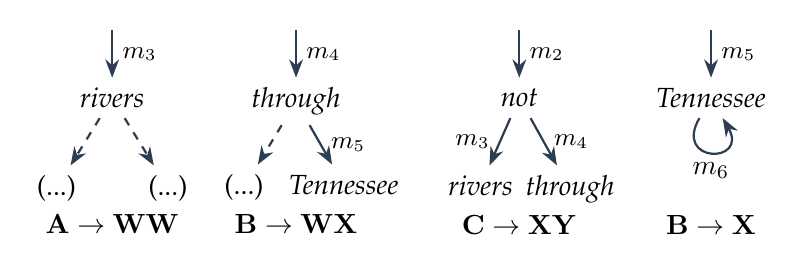
\begin{tikzpicture}[node distance=6.0mm and 28mm, >=Stealth, 
	semantic/.style={draw=none, minimum height=5mm, rectangle},
	word/.style={draw=none, minimum height=5mm, rectangle},
	olabel/.style={draw=none, circle, minimum height=9mm, minimum width=9mm,line width=1pt, inner sep=2pt, fill=lowblue, text=fontgray, label={center:\textsc{o}}},
	bperlabel/.style={draw=none, circle, minimum height=9mm, minimum width=9mm,line width=1pt, inner sep=2pt, fill=lowblue, text=black, label={center:\textsc{per}}},
	borglabel/.style={draw=none, circle, minimum height=9mm, minimum width=9mm,line width=1pt, inner sep=2pt, fill=lowblue, text=black, label={center:\textsc{org}}},
	bgpelabel/.style={draw=none, circle, minimum height=9mm, minimum width=9mm,line width=1pt, inner sep=2pt, fill=lowblue, text=black, label={center:\textsc{Misc}}},
	nnlabel/.style={draw=none, circle, minimum height=9mm, minimum width=9mm,line width=1pt, inner sep=2pt, fill=mypumpkin, text=black, label={center:\textsc{Gpe}}},
	invis/.style={draw=none, circle,line width=0pt, inner sep=0pt, fill=none, text=fontgray},
	chainLine/.style={line width=0.8pt,->, color=fontgray}	%		,background rectangle/.style={fill=olive!45}, show background rectangle
	]
	\node[invis](riversparent) {};
	\node[word, below = of riversparent](rivers) {{\em rivers}};
	\draw [chainLine] (riversparent) to [] node[right, color=black] {\small  $m_3$} (rivers);
	\node[word, below left = of rivers, xshift=30mm,yshift=0mm](riversleft) {(...)};
	\node[word, below right = of rivers, xshift=-30mm,yshift=0mm](riversright) {(...)};
	\draw [chainLine, dashed] (rivers) to [] node[right, color=black] {} (riversleft);
	\draw [chainLine, dashed] (rivers) to [] node[right, color=black] {} (riversright);
	
	\node[invis, right =of riversparent, xshift=-5mm](throughparent) {};
	\node[word, below = of throughparent](through) {{\em through}};
	\node[word, below right = of through, xshift=-37mm,yshift=1mm](tn) {{\em Tennessee}};
	\node[word, below left = of through, xshift=32mm,yshift=1mm](tnleft) {(...)};
	\draw [chainLine] (throughparent) to [] node[right, color=black] {\small  $m_4$} (through);
	\draw [chainLine] (through) to [] node[right, color=black] {\small  $m_5$} (tn);
	\draw [chainLine, dashed] (through) to [] node[right, color=black] {} (tnleft);
	
	\node[invis, right =of throughparent](notparent) {};
	\node[word, below = of notparent](not) {{\em not}};
	\node[word, below left = of not, xshift=32mm](rivers2) {{\em rivers}};
	\node[word, below right = of not, xshift=-32mm](through2) {{\em through}};
	
	
	\draw [chainLine] (notparent) to [] node[right, color=black] {\small  $m_2$} (not);
	\draw [chainLine] (not) to [] node[left, color=black] {\small  $m_3$} (rivers2);
	\draw [chainLine] (not) to [] node[right, color=black] {\small  $m_4$} (through2);
	
	\node[invis, right =of notparent, xshift=-4mm](tnparent) {};
	\node[word, below = of tnparent](tn2) {{\em Tennessee}};
	
	\draw [chainLine] (tnparent) to [] node[right, color=black] {\small  $m_5$} (tn2);
	\draw [chainLine]  (tn2) to [out=-120,in=-60, looseness=5.8] node[below, yshift=0mm, color=black]{$m_6$} (tn2);
	
	\node[word, below = of rivers, yshift=-4.9mm](a) {$\mathbf{A} \rightarrow \mathbf{W}\mathbf{W}$};
	\node[word, below = of through, yshift=-4mm](a) {$\mathbf{B} \rightarrow \mathbf{W}\mathbf{X}$};
	\node[word, below = of not, yshift=-5mm](a) {$\mathbf{C} \rightarrow \mathbf{X}\mathbf{Y}$};
	\node[word, below = of tn2, yshift=-5mm](a) {$\mathbf{B} \rightarrow \mathbf{X}$};
	\end{tikzpicture}
	%	}
	%	\vspace{-2mm}
	\caption{Example dependency  patterns used in the {dependency-based hybrid tree} of Figure \ref{fig:dhtexample}.}
	%	\vspace{-2mm}
	\label{fig:patternexample}
\end{figure}

Based on the dependency patterns, we are able to define the set of all possible allowable {\em dependency-based hybrid tree} representations. Each representation  essentially belongs to a class of {\em projective} dependency trees where semantic units appear on the dependency arcs and (some of the) words are selected as nodes. The semantic tree can be constructed by following the arcs while referring to the dependency patterns involved.

%, we introduce the $\mathbf{B} \rightarrow \mathbf{X}$

%In order to allow some of the words to have no parent and recurrence to happen in our dependency-based hybrid tree representation, we define some patterns during the construction of such dependency-based hybrid tree. 
%For example at the bottom of Figure \ref{fig:dhtexample}, $m_2$ has two arguments, we then allow two dependency arcs starts from the word ``\textit{not}''. 
%One goes to the left-hand side of ``\textit{not}'' (i.e., ``\textit{not}'' to ``\textit{rivers}'') and the other one goes to the right-hand side of ``\textit{not}'' (i.e., ``\textit{not}'' to ``\textit{through}''). 

%Specifically, Table \ref{tab:patterns} shows the patterns allowed to appear in our model. 
%Later in Section \ref{sec:learninganddecode}, we show how the efficient training algorithm benefits from such patterns. 
%First of all, we use $\mathbf{A}$, $\mathbf{B}$ or $\mathbf{C}$ to denote the pattern of a semantic unit which has 0, 1 or 2 arguments, respectively. 
%$\mathbf{W}$ refers to a contiguous span of words that are immediately associated with the current semantic unit. 
%$\mathbf{X}$ and $\mathbf{Y}$ refer to a contiguous span of words that map to the first and second child semantic unit, respectively\footnote{Our patterns are similar to those used in \textit{relaxed hybrid tree}~\cite{lu2015constrained}  and we require much less amount of patterns used in our model}. 
%
%For example, the $m_2$ with two arguments in Figure \ref{fig:dhtexample} follows the pattern $\mathbf{C} \rightarrow \mathbf{XY}$, which means the sequence of words on the left-hand side of ``{\em not}'' follow pattern $\mathbf{X}$ and the words on the right-hand side ``{\em not}'' follow pattern $\mathbf{Y}$. 
%The choice of $\mathbf{XY}$ or $\mathbf{YX}$ is based on the children order. 
%If the first child semantic unit is $m_4$ and the second is $m_3$, the pattern would be $\mathbf{YX}$. 
%The other example is $m_4$ with one argument. 
%The mapping follows the pattern $\mathbf{B} \rightarrow \mathbf{WX}$ where the words at left-hand side {\em immediately} associate to $m_4$ and the words at the right-hand side map to the child semantic unit $m_5$. 
%More details are described in Section \ref{sec:learninganddecode}. 

%As we also allow the recurrence to appear in our hybrid tree representation, $\mathbf{X}$ pattern for semantic units (i.e., $\mathbf{B}$) with one argument is introduced\footnote{The limitations of disallowing such a pattern have been discussed in previous work~\cite{lu2015constrained}.}. 
%In order to avoid infinite recurrence of semantic units on a word, we set a maximum height $c$ to restrict the maximum number of recurrences. 

{\color{red}
}


\subsection{Model}

%OK

Given the natural language words $\boldsymbol{n}$, our task is to predict  $\boldsymbol{m}$, which is a tree-structured meaning representation, consisting of a set of semantic units as the nodes in the semantic tree. 
%We also need to predict latent 
We use  $\boldsymbol{t}$ to denote a dependency-based hybrid tree (as shown in Figure \ref{fig:dhtexample}), which jointly encodes both natural language words and the gold meaning representation.  
%As we can see from the figure, the dependency tree $\boldsymbol{t}$ consists of a set of dependency arcs which can be represented by a triple $(n_p, n_c, m)$, where $n_p$ is the parent, $n_c$ is the child and $m$ is the dependency relation (i.e., semantic unit). 
Let $\mathcal{T}(\boldsymbol{n}, \boldsymbol{m})$ denote all the possible dependency-based hybrid trees that contain the natural language words $\boldsymbol{n}$ and the meaning representation $\boldsymbol{m}$. 
We adopt the widely-used structured prediction model conditional random fields (CRF)~\cite{lafferty2001conditional}. 
The  probability of a possible meaning representation $\boldsymbol{m}$ and dependency-based hybrid tree $\boldsymbol{t}$ for a sentence $\boldsymbol{n}$ is given by:
\begin{equation}
P_\vec{w} (\boldsymbol{m}, \boldsymbol{t} | \boldsymbol{n}) 
= 
\frac{
	e ^{\vec{w}\cdot \vec{f} (\boldsymbol{n}, \boldsymbol{m}, \boldsymbol{t})}
}
{
	\sum_{\boldsymbol{m}^\prime, \boldsymbol{t}^\prime \in \mathcal{T}(\boldsymbol{n}, \boldsymbol{m}^\prime )} 
	e^{\vec{w} \cdot \vec{f} (\boldsymbol{n}, \boldsymbol{m}^\prime, \boldsymbol{t}^\prime)}
}\nonumber
\label{equ:joint}
\end{equation}
where $\vec{f}(\boldsymbol{n}, \boldsymbol{m}, \boldsymbol{t})$ is the feature vector defined over the $(\boldsymbol{n}, \boldsymbol{m}, \boldsymbol{t})$ tuple,
% input $\boldsymbol{n}$, meaning representation $\boldsymbol{m}$ and the dependency tree $\boldsymbol{t}$ 
and $\vec{w}$ is the parameter vector.
% of the features. 
Since we do not have the knowledge of the ``true'' dependencies during training, $\boldsymbol{t}$ is regarded as a latent-variable in our model. 
We marginalize $\boldsymbol{t}$ in the above equation and the resulting model is a latent-variable CRF~\cite{quattoni2005conditional}:
% shown in Equation \ref{equ:latent} where the distribution defined on a particular $(\boldsymbol{n}, \boldsymbol{m})$ pair. 
\begin{equation}
\begin{split}
P_\vec{w} (\boldsymbol{m} | \boldsymbol{n}) 
&= 
\sum_{\boldsymbol{t} \in \mathcal{T} (\boldsymbol{n}, \boldsymbol{m}) }  
P_\vec{w} (\boldsymbol{m}, \boldsymbol{t} | \boldsymbol{n})  \\
& = \frac{
	\sum_{\boldsymbol{t} \in \mathcal{T} (\boldsymbol{n}, \boldsymbol{m}) }	
	e ^{\vec{w} \cdot \vec{f} (\boldsymbol{n}, \boldsymbol{m}, \boldsymbol{t})}
}
{
	\sum_{\boldsymbol{m}^\prime, \boldsymbol{t}^\prime \in \mathcal{T}(\boldsymbol{n}, \boldsymbol{m}^\prime )} 
	e^{\vec{w} \cdot \vec{f} (\boldsymbol{n}, \boldsymbol{m}^\prime, \boldsymbol{t}^\prime)}
}
\end{split}
\label{equ:latent}
\end{equation}

Given a dataset $\mathcal{D}$ of $(\boldsymbol{n}, \boldsymbol{m})$ pairs, our objective is to minimize the negative log-likelihood:\footnote{We ignore the $L_2$ regularization term for brevity.}
\begin{equation}
\begin{split}
%\mathcal{L} (\vec{w})
%=
%-
%\sum_{(\vec{n}, \vec{m}) \in \mathcal{D}}
%\log P_\vec{w}(\vec{m} | \vec{n})
%+ \lambda ||\vec{w}||^2 \\
\mathcal{L} (\vec{w}) = 
-  \!\!\!\!\!\!
\sum_{(\boldsymbol{n}, \boldsymbol{m}) \in \mathcal{D}}
\!\!\!
\log
\!\!
\sum_{\boldsymbol{t} \in \mathcal{T} (\boldsymbol{n}, \boldsymbol{m}) }  
\!\!
P_\vec{w} (\boldsymbol{m}, \boldsymbol{t} | \boldsymbol{n})
%+ \lambda ||\vec{w}||^2 
\end{split}
\label{equ:obj}
\end{equation}
%where $\lambda$ is the coefficient for the regularization. 


The gradient for  model parameter $w_k$ is:
\begin{align}
\frac{\partial \mathcal{L}(\vec{w})}{\partial w_k}
&=\!\!\!\!\!\!\!
\sum_{(\boldsymbol{n}, \boldsymbol{m}) \in \mathcal{D}}
\sum_{\boldsymbol{m}^\prime, \boldsymbol{t} }
\mathbf{E}_{P_\vec{w}(\vec{m}^\prime, \boldsymbol{t} | \boldsymbol{n}) }
[ f_k (\boldsymbol{n}, \boldsymbol{m}, \boldsymbol{t}) ]\nonumber\\
& - \!\!\!\!\!
\sum_{(\boldsymbol{n}, \boldsymbol{m}) \in \mathcal{D}}
\sum_{\boldsymbol{t} }
\mathbf{E}_{P_\vec{w}(\boldsymbol{t} | \boldsymbol{n}, \boldsymbol{m}) }
[ f_k (\boldsymbol{n}, \boldsymbol{m}, \boldsymbol{t}) ]\nonumber
%+ 2\lambda w_k\nonumber
\end{align}
where $f_k (\boldsymbol{n}, \boldsymbol{m}, \boldsymbol{t})$ represents the number of occurrences of the $k$-th feature. 
With both the objective and gradient above, we can minimize the objective function with standard optimizers, such as L-BFGS~\cite{liu1989limited}  and stochastic gradient descent. 
Calculation of these expectations involves all possible dependency-based hybrid trees.
As there are exponentially many such trees, 
an efficient inference procedure is required.
% for calculating  the objective and gradients.
We will present our efficient algorithm to perform  exact inference for learning and decoding in the next section. 
%Such efficient inference procedures would allow us to calculate the objective and gradients efficiently.


\subsection{Learning and Decoding}
\label{sec:learninganddecode}

We propose  dynamic-programming algorithms to perform efficient and exact inference, which will be used for calculating the objective and gradients discussed in the previous section.
The algorithms are inspired by the inside-outside style algorithm~\cite{baker1979trainable}, graph-based dependency parsing~\cite{eisner2000bilexical,koo2010efficient,shi2017fast}, and the \textit{relaxed hybrid tree} model~\cite{lu2014semantic,lu2015constrained}. 
As discussed in Section \ref{sec:patterns}, our latent dependency trees are {projective} as in traditional dependency parsing~\cite{eisner1996three,nivre2004deterministic,mcdonald2005online} -- the dependencies are non-crossing with respect to the word order (see bottom of Figure \ref{fig:example}). 


The objective function in Equation \ref{equ:obj} can be further decomposed into the following form\footnote{Regularization term is excluded for brevity.}:
\begin{equation}
\begin{split}
\mathcal{L} (\vec{w})
=
-
\sum_{(\boldsymbol{n}, \boldsymbol{m}) \in \mathcal{D}}
\log \sum_{\boldsymbol{t} \in \mathcal{T} (\boldsymbol{n}, \boldsymbol{m}) }	
e ^{\vec{w} \cdot \vec{f} (\boldsymbol{n}, \boldsymbol{m}, \boldsymbol{t})} 
+
\sum_{(\boldsymbol{n}, \boldsymbol{m}) \in \mathcal{D}}
\!\!\!
\log
\sum_{\boldsymbol{m}^\prime, \boldsymbol{t}^\prime \in \mathcal{T}(\boldsymbol{n}, \boldsymbol{m}^\prime )} 
e^{\vec{w} \cdot \vec{f} (\boldsymbol{n}, \boldsymbol{m}^\prime, \boldsymbol{t}^\prime)}\nonumber
\end{split}
\label{equ:objdecompose}
\end{equation}

We can see the first term is essentially the combined score of all the possible latent structures containing the pair $(\boldsymbol{n}, \boldsymbol{m})$. 
The second term is the combined score for all the possible latent structures containing $\boldsymbol{n}$. 
%We show how such scores can be factorized through an inside-outside style procedure similar to graph-based dependency parsing~\cite{eisner2000bilexical,koo2010efficient}.
We show how such scores can be calculated in a factorized manner, based on the fact that we can recursively decompose a dependency-based hybrid tree based on the dependency patterns we introduced.
% into individual dependency arcs.

Formally, we introduce two interrelated dynamic-programming structures that are similar to those used in graph-based dependency parsing~\cite{eisner2000bilexical,koo2010efficient,shi2017fast}, namely {\em complete span} and {\em complete arc span}. 
Figure \ref{fig:modelderivation}a shows an example of {\em complete span} (left) and {\em complete arc span} (right). 
The {\em complete span} (over $[i,j]$) consists of a headword (at $i$) and its descendants on one side (they altogether form a subtree), a dependency pattern and a semantic unit. 
The {\em complete arc span} is a span (over $[i,j]$) with a dependency between the headword (at $i$) and the modifier (at $k$). 
We use $C_{i,j,p,m}$ to denote a complete span, where $i$ and $j$ represent the indices of the headword and endpoint, $p$ is the dependency pattern and $m$ is the semantic unit. 
Analogously, we use $A_{i,k,j,p,m}$ to denote a complete arc span where $i$ and $k$ are used to denote the additional dependency from the word at the $i$-th position as headword to the word at the $k$-{th} position as modifier. 


\begin{figure}[t!]
	\centering
	\begin{subfigure}{0.6\linewidth}
		
		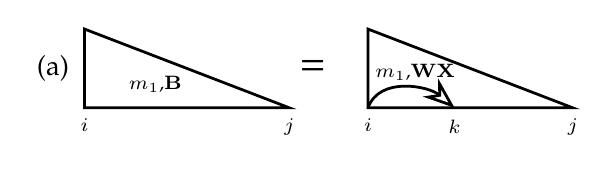
\begin{tikzpicture}
		\node [scale = 1](a) at (-0.6,0.5) {(a)};
		\draw [line width = 1pt] (2.4,0) node [below] {\scriptsize $j$} -- (-0.2,0) node [below] {\scriptsize $i$} -- (-0.2,1) -- cycle;
		\node [](pa_type1) at (0.7, 0.3) {\scriptsize $m_1$,$ \mathbf{B}$};
		\node [scale = 1.5](equals) at (2.7, 0.5) {=};
		\draw [line width = 1pt] (6.0,0) node [below] {\scriptsize $j$} -- (3.4,0) node [below] {\scriptsize $i$} -- (3.4,1)-- cycle;
		\node [](type) at (4.0, 0.45) {\scriptsize $m_1$,$\mathbf{WX}$};
		\draw [line width=1pt, -{Stealth[length=4mm, open]}] (3.4,0) to [out=70,in=140] node [above] {} (4.5,0);
		\node [](type) at (4.5, -0.24) {\scriptsize $k$};
		\end{tikzpicture}
	\end{subfigure}
	
	\begin{subfigure}{0.6\linewidth}
		
		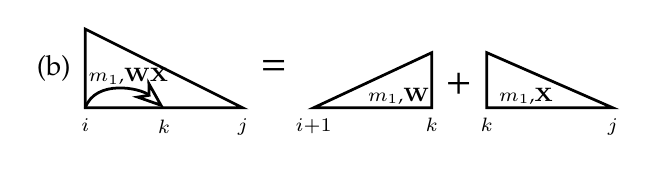
\begin{tikzpicture}
		\node [scale = 1](a) at (-0.6,0.5) {(b)};
		\draw [line width = 1pt] (1.8,0) node [below] {\scriptsize $j$} -- (-0.2,0) node [below] {\scriptsize $i$} -- (-0.2,1) -- cycle;
		\node [](k) at (0.8, -0.24) {\scriptsize $k$};
		\draw [line width=1pt, -{Stealth[length=4mm, open]}] (-0.2,0) to [out=70,in=140] node [above] {} (0.8, 0);
		\node [](type) at (0.35, 0.4) {\scriptsize $m_1$,$\mathbf{WX}$};
		\node [scale = 1.5](equals) at (2.2,0.5) {=};
		\draw [line width = 1pt] (4.2,0) node [below] {\scriptsize $k$} -- (2.7,0) node [below] {\scriptsize $i$$+$$1$}-- (4.2,0.7) -- cycle;
		\node [](pa_type1) at (3.78, 0.15) {\scriptsize $m_1$,$\mathbf{W}$};
		\node [scale = 1.5](equals) at (4.55,0.3) {+};
		\draw [line width = 1pt] (6.5,0) node [below] {\scriptsize $j$} -- (4.9,0) node [below] {\scriptsize $k$} -- (4.9,0.7) -- cycle;
		\node [](pa_type2) at (5.4, 0.15) {\scriptsize $m_1$,$\mathbf{X}$};
		\end{tikzpicture}
	\end{subfigure}
	\begin{subfigure}{0.6\linewidth}
		
		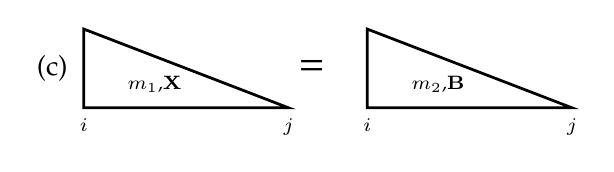
\begin{tikzpicture}
		\node [scale = 1](a) at (-0.6,0.5) {(c)};
		\draw [line width = 1pt] (2.4,0) node [below] {\scriptsize $j$} -- (-0.2,0) node [below] {\scriptsize $i$} -- (-0.2,1) -- cycle;
		\node [](pa_type1) at (0.7, 0.3) {\scriptsize $m_1$,$\mathbf{X}$};
		\node [scale = 1.5](equals) at (2.7, 0.5) {=};
		\draw [line width = 1pt] (6.0,0) node [below] {\scriptsize $j$} -- (3.4,0) node [below] {\scriptsize $i$} -- (3.4,1)-- cycle;
		\node [](type) at (4.3, 0.3) {\scriptsize $m_2$,$\mathbf{B}$};
		\end{tikzpicture}
	\end{subfigure}
	\begin{subfigure}{0.6\linewidth}
		
		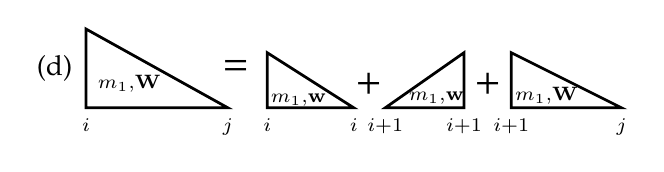
\begin{tikzpicture}
		\node [scale = 1](a) at (-0.6,0.5) {(d)};
		\draw [line width = 1pt] (1.6,0) node [below] {\scriptsize $j$} -- (-0.2,0) node [below] {\scriptsize $i$} -- (-0.2,1) -- cycle;
		\node [](type) at (0.35, 0.3) {\scriptsize $m_1$$,$$\mathbf{W}$};
		\node [scale = 1.5](equals) at (1.7,0.5) {=};
		\draw [line width = 1pt] (3.2,0) node [below] {\scriptsize $i$} -- (2.1,0.0) node [below] {\scriptsize $i$}-- (2.1,0.7) -- cycle;
		\node [](pa_type1) at (2.5, 0.1) {\scriptsize $m_1$$,$$\mathbf{w}$};
		\node [scale = 1.5](equals) at (3.4,0.3) {+};
		\draw [line width = 1pt] (4.6,0) node [below] {\scriptsize $i$$+$$1$} -- (3.6,0) node [below] {\scriptsize $i$$+$$1$} -- (4.6,0.7) -- cycle;
		\node [](pa_type2) at (4.25, 0.12) {\scriptsize $m_1$$,$$\mathbf{w}$};
		\node [scale = 1.5](equals) at (4.9,0.3) {+};
		\draw [line width = 1pt] (6.6,0) node [below] {\scriptsize $j$} -- (5.2,0.0) node [below] {\scriptsize $i$$+$$1$}-- (5.2,0.7) -- cycle;
		\node [](pa_type2) at (5.65, 0.15) {\scriptsize $m_1$$,$$\mathbf{W}$};
		\end{tikzpicture}
	\end{subfigure}
	%	\vspace{-2mm}
	\caption{The dynamic-programing structures and derivation of our model. The other direction is symmetric. See supplementary material for the complete structures.}
	%	\vspace{-3.8mm}
	\label{fig:modelderivation}
\end{figure}



As we can see from the derivation in Figure \ref{fig:modelderivation}, each type of span can be constructed from smaller spans in a bottom-up manner.  
Figure \ref{fig:modelderivation}a shows that a {complete span} is constructed from a {complete arc span} following the dependency patterns in Table \ref{tab:patterns}. 
Figure \ref{fig:modelderivation}b shows a {complete arc span} can be simply constructed from two smaller complete spans based on the dependency pattern.  
In Figure \ref{fig:modelderivation}c and \ref{fig:modelderivation}d, we further show how such two complete spans with pattern $\mathbf{X}$ (or $\mathbf{Y}$) and $\mathbf{W}$ can be constructed.
Figure \ref{fig:modelderivation}c illustrates how to model a transition from one semantic unit to another where the parent is $m_1$ and the child is $m_2$ in the semantic tree. 
If $m_2$ has arity 1, then the pattern is $\mathbf{B}$ following the dependency patterns in Table \ref{tab:patterns}. 
For spans with a single word, we use the lowercase $\mathbf{w}$ as the pattern to indicate this fact, as shown in Figure \ref{fig:modelderivation}d. 
They are the atomic spans used for building larger spans. 
As the {complete span} in Figure \ref{fig:modelderivation}d is associated with pattern $\mathbf{W}$, which means the words within this span are under the semantic unit $m_1$, we can incrementally construct this span with atomic spans.
We illustrate the construction of a complete dependency-based hybrid tree in the supplementary material. 


Our final goal during training for a sentence $\boldsymbol{n}=\{w_0, w_1,\cdots, w_N\}$ is to construct all the possible {\em complete spans} that cover the interval $[0, N]$, which can be represented as $C_{0,N,\cdot, \cdot}$. 
Similar to the chart-based dependency parsing algorithms~\cite{eisner1996three,eisner2000bilexical,koo2010efficient}, we can obtain the {\em inside} and {\em outside} scores using our dynamic-programming derivation in Figure \ref{fig:modelderivation} during the inference process,
which can then be used to calculate the objective and feature expectations. 
Since the spans are defined by at most three free indices, the dependency pattern and the semantic unit, our dynamic-programming algorithm requires $\mathcal{O}(N^3M)$ time\footnote{We omit a small constant factor associated with patterns.} where $M$ is the number of semantic units. 
The resulting complexity is the same as the {relaxed hybrid tree} model~\cite{lu2014semantic}. 

%the number of pattern as it is small as shown in Table \ref{tab:patterns}.

%We use $\alpha ( C_{i,j,p,m} )$ denotes the {\em inside} scores (in exponential space) of all the possible dependency-based hybrid trees that are rooted at $m$, with word association pattern $p$ and covering span $(w_i, \cdots, w_j)$. 
%
%We use Figure \ref{fig:dhtexample}a and \ref{fig:dhtexample}b to illustrate how these scores are computed using the dynamic programming structures. 
%The {\em inside} score derivations are similar to the one in {\em relaxed hybrid tree}~\cite{lu2014semantic} and dynamic-programing-based dependency parsing~\cite{koo2010efficient,shi2017fast}. 
%\begin{equation}
%\begin{split}
%\alpha (C^r_{i,j,p,m})  & = \sum_{p^\prime \in children(p)} \sum_{k=i+1}^{j} \alpha(A^r_{i,k,j,p^\prime,m}) \\
%\alpha(A^r_{i,k,j,p,m}) & = \alpha (C^l_{i+1, k, pc_1, m}) \otimes  \alpha (C^r_{k, j, pc_1, m})  \nonumber 
%\end{split}
%\end{equation}
%where the $\otimes$ operation 
%
%Finally, the inside score for a specific span $n= (w_i, \cdots, w_j)$ rooted at $m$ can be calculated by:
%\begin{equation}
%\alpha \big( C^r_{i, j,\cdot,m}\big) = \sum_p \alpha \big( C^r_{i, j,p,m}\big)
%\end{equation}
%
%
%
%It is clear to see that the above dynamic-programming algorithm have a complexity of $\mathcal{O}(n^3T)$ where $T$ is the number of semantic units and the complexity is same as the \textit{hybrid tree} model~\cite{lu2014semantic}. 
%
%For a sentence $\vec{n}$ with 

During decoding, we can find the optimal (tree-structured) meaning representation $\boldsymbol{m}^*$ for a given  input sentence $\boldsymbol{n}$ by the Viterbi algorithm. 
This step can also be done efficiently with our dynamic-programming approach, where we switch from marginal inference to MAP inference:
\begin{equation}
\boldsymbol{m}^*, \boldsymbol{t}^* = \argmax_{\boldsymbol{m}, \boldsymbol{t}\in\mathcal{T} (\boldsymbol{n}, \boldsymbol{m})} e ^{\vec{w} \cdot \vec{f} (\boldsymbol{n}, \boldsymbol{m}, \boldsymbol{t})}
\end{equation}
%\begin{center}
%	\begin{tabular}{c}
%		$
%		 \boldsymbol{m}^*, \boldsymbol{t}^* = \argmax_{\boldsymbol{m}, \boldsymbol{t}\in\mathcal{T} (\boldsymbol{n}, \boldsymbol{m})} e ^{\vec{w} \cdot \vec{f} (\boldsymbol{n}, \boldsymbol{m}, \boldsymbol{t})}
%		$
%	\end{tabular}
%\end{center}
%\begin{equation}
%\begin{split}
%\boldsymbol{m}^*, \boldsymbol{t}^* 
%%& = \argmax_{\boldsymbol{m}, \boldsymbol{t}\in\mathcal{T} (\boldsymbol{n}, \boldsymbol{m})}  P_\vec{w}(\boldsymbol{m}, \boldsymbol{t} | \boldsymbol{n}) \\
%& = \argmax_{\boldsymbol{m}, \boldsymbol{t}\in\mathcal{T} (\boldsymbol{n}, \boldsymbol{m})} e ^{\vec{w} \cdot \vec{f} (\boldsymbol{n}, \boldsymbol{m}, \boldsymbol{t})}
%\end{split}
%\end{equation}
%\begin{equation}
%\begin{split}
%\vec{m}^* & = \argmax_\vec{m} P_\vec{w}(\vec{m} | \vec{n}) \\
%& = \argmax_\vec{m} \sum_{\vec{t} \in \mathcal{T} (\vec{n}, \vec{m})} 
%P_\vec{w}(\vec{m}, \vec{t} | \vec{n}) \\
%& = \argmax_\vec{m} \sum_{\vec{t} \in \mathcal{T} (\vec{n}, \vec{m})}  
%e ^{\vec{w} \cdot \vec{f} (\vec{n}, \vec{m}, \vec{t})}
%\end{split}
%\end{equation}
%In order to use a dynamic-programming procedure similar to the training process, we replace the $\sum$ operation with $\max$. 
%We can jointly find the optimal meaning representation $\vec{m}^*$ together with the optimal dependency tree $\vec{t}$ by the following:
%\begin{equation}
%\begin{split}
%\vec{m}^*, \vec{t}^* 
%& = \argmax_{\vec{m}, \vec{t}\in\mathcal{T} (\vec{n}, \vec{m})}  e ^{\vec{w} \cdot \vec{f} (\vec{n}, \vec{m}, \vec{t})} \\
%& = \argmax_{\vec{m}, \vec{t}\in\mathcal{T} (\vec{n}, \vec{m})} \vec{w} \cdot \vec{f} (\vec{n}, \vec{m}, \vec{t})
%\end{split}
%\end{equation}
A similar decoding procedure has been used in previous work~\cite{lu2014semantic,durrett2015neural} with CKY-based parsing algorithm.
%The underlying procedure was also used in previous work~\cite{lu2014semantic,susanto2017semantic}. 
%We can then use Viterbi algorithm find the optimal meaning representation $\vec{m}^*$ as well as the optimal dependency tree $\vec{t}^*$ that contains the $\vec{m}^*$. 

%{\color{red}
%}







\subsection{Features}
\label{sec:features}
As shown in Equation \ref{equ:joint}, the features are defined on the tuple $(\boldsymbol{n}, \boldsymbol{m}, \boldsymbol{t})$. 
With the dynamic-programming procedure, we can define the features over the structures in Figure \ref{fig:dhtexample}. 
Our feature design is inspired by the {hybrid tree} model~\cite{lu2015constrained} and graph-based dependency parsing~\cite{mcdonald2005online}. 
Table \ref{tab:features} shows the feature templates for the example in Figure \ref{fig:dhtexample}. 
Specifically, we define simple unigram features (concatenation of a semantic unit and a word that directly appears under the unit), pattern features (concatenation of the semantic unit and the child pattern) and transition features (concatenation of the parent and child semantic units). 
They form our basic feature set. 


\begin{table}[t!]
	\centering
%	\scalebox{1.0}{
		\begin{tabular}{lc}
			\toprule
			Feature Type & Examples \\
			\midrule
			\midrule
			Word &  ``$m_4$ \& {\em run}'', ~~``$m_4$ \& {\em through}'' \\
			Pattern & ``$m_2$ \& $\mathbf{XY}$'', ~~``$m_4$ \& $\mathbf{WX}$'' \\
			Transition & ``$m_2$ \& $m_3$'', ~~``$m_2$ \& $m_4$'' \\
			\midrule
			\midrule 
			Head word & ``$m_2$ \& {\em What}'', ~~``$m_4$ \& {\em not}'' \\
			Modifier word & ``$m_2$ \& {\em not}'', ~~``$m_4$ \& {\em through}'' \\
			Bag of words & ``$m_4$ \& {\em not}'', ~~``$m_4$ \& {\em run}'', ~~``$m_4$ \& {\em through}'' \\
			\bottomrule 
		\end{tabular}
%	}
	%	\vspace{-2mm}
	\caption{Features for the example in Figure \ref{fig:dhtexample}. 
		%	Bottom shows the dependency-related features.
	}
	%	\vspace{-3mm}
	\label{tab:features}
\end{table}

Additionally, with the structured properties of dependencies, we can define dependency-related features~\cite{mcdonald2005online}. 
%We use the parent and child words head (parent) and modifier (child) words of the dependency as features. 
We use the parent (head) and child (modifier) words of the dependency as features.
We also use the bag-of-words covered under a dependency as features. 
The dependency features are useful in helping improve the performance as we can see in the experiments section. 
%We present  examples of features in the supplementary material.



\subsection{Neural Component}

Following the approach used in \citet{susanto2017semantic}, we could further incorporate  neural networks into our latent-variable graphical model. 
The integration is analogous to the approaches described in the neural CRF models~\cite{artieres2010neural,durrett2015neural,gormley2015graphical,lample2016neural},
where we use neural networks to learn distributed feature representations within our graphical model.

%\begin{figure}[t!]
%	\centering
%	\begin{tikzpicture}[node distance=4mm and 4mm, >=Stealth, 	place/.style={draw=none, inner sep=2pt,line width=0.8pt},
%	invis/.style={draw=none, circle,line width=0pt, inner sep=0pt, fill=none, text=fontgray}]
%	\node [place](wleft) [] {$w_{p}$};
%	
%	
%	\node [draw, line width=0.8pt, rectangle, minimum width=0.4pt, minimum height=20pt, rounded corners=0.2pt] (wleftembed) [right=of wleft] {};
%	\node [draw, line width=0.8pt, rectangle, minimum width=0.4pt, minimum height=20pt, rounded corners=0.2pt] (wrightembed) [below=of wleftembed] {};
%%	\node [place](wmiddle) [left=of wmiddleembed] {$w_{t}$};
%	\node [place](wright) [left=of wrightembed] {$w_{c}$};
%	
%	\draw [line width=0.8pt, ->] (wleft) to [] node [] {} (wleftembed);
%%	\draw [line width=1pt, ->] (wmiddle) to [] node [] {} (wmiddleembed);
%	\draw [line width=0.8pt, ->] (wright) to [] node [] {} (wrightembed);
%	
%	%hidden layer
%	\node [draw, line width=0.8pt, rectangle, text width=11mm, minimum height=50pt, rounded corners=1pt,xshift=5mm, yshift=-4mm] (hidden) [right=of wleftembed] {\small Bilinear\\~~~$\mathbf{U}$};
%	\node [place, text width=23pt, font=\small, align=center, yshift =3mm](hiddenword) [below=of hidden] {};
%	
%	\draw [line width=0.8pt, ->] (wleftembed) to [] node [above, font=\small] {$\vec{e}_{p}$} (hidden);
%%	\draw [line width=1pt, ->] (wmiddleembed) to [] node [above, font=\small, yshift=-1mm, xshift=-1mm] {$\vec{e}_{t}$} (hidden);
%	\draw [line width=0.8pt, ->] (wrightembed) to [] node [below, font=\small, xshift=1mm] {$\vec{e}_{c}$} (hidden);
%	
%	\node [draw=none, line width=0.8pt, minimum width=0.4pt, minimum height=50pt, rounded corners=1pt,xshift=5mm] (output) [right=of hidden] {};
%%	\node [place, text width=23pt, font=\small, align=center, yshift =3mm](outputword) [below=of output] {output layer};
%	\draw [line width=0.8pt, ->] (hidden) to [] node [above] {} (output);
%	
%	\end{tikzpicture}
%	\caption{Our bilinear neural architecture.}
%	\label{fig:neural}
%\end{figure}
%As the semantic units are defined on the dependencies, w
We employ a neural architecture to calculate the score associated with each dependency arc $(w_p, w_c, m)$ (here $w_p$ and $w_c$ are the parent and child words in the dependency and $m$ is the semantic unit over the arc), where the input to the neural network consists of  words (i.e., $(w_p, w_c)$) associated with this dependency and the neural network will calculate a score for each possible semantic unit, including $m$.
% the score of the semantic unit $m$. 
The two words are first mapped to word embeddings  $\vec{e}_p$ and $\vec{e}_c$ (both of dimension $d$). 
Next, we use a bilinear layer\footnote{Empirically, we also tried multilayer perceptron but the bilinear model gives us better results.}~\cite{socher2013recursive,chen2016thorough} to capture the interaction between the parent and the child in a dependency:
\begin{equation*}
r_i = \vec{e}_p^{\mathbf{T}} \mathbf{U}_i \vec{e}_c
\end{equation*}
%\begin{center}
%	\begin{tabular}{c}
%		$
%		r_i = \vec{e}_p^{\mathbf{T}} \mathbf{U}_i \vec{e}_c
%		$
%	\end{tabular}
%\end{center}
where $r_i$ represents the score for the $i$-th semantic unit and $\mathbf{U}_i \in \mathbb{R}^{d\times d}$.
The scores are then incorporated into the probability expression in Equation \ref{equ:joint} during learning and decoding.
As a comparison, we also implemented a  variant where our model directly takes in the average embedding of $\mathbf{e}_p$ and $\mathbf{e}_c$ as additional features, without using our neural component. 

%We implemented two neural architectures: multilayer perceptron (MLP) and bilinear networks. 
%The MLP architecture is also used in the {\it neural hybrid tree} model~\cite{susanto2017semantic}. 
%However, the window size in their MLP can differ in terms of the language, which may not be robust. 
%Our MLP and bilinear architectures do not require the window size. 






\section{Experiments}

\paragraph{Data and evaluation methodology} 

We conduct experiments on the publicly available variable-free version of the GeoQuery dataset, which has been widely used for semantic parsing~\cite{wong2006learning,lu2008generative,jones2012semantic}. 
The dataset consists of 880 pairs of natural language sentences and the corresponding tree-structured semantic representations. 
This dataset is annotated with eight languages. 
%This dataset is annotated with eight languages~\cite{jones2012semantic,lu2011probabilistic,susanto2017semantic}.  
The original annotation of this dataset is English~\cite{zelle1996learning} and \citet{jones2012semantic} annotated the dataset with three more languages: German, Greek and Thai. 
\citet{lu2011probabilistic} released the Chinese annotation and \citet{susanto2017semantic} annotated the corpus with three additional languages: Indonesian, Swedish and Farsi. 
In order to compare with previous work~\cite{jones2012semantic,lu2015constrained}, we follow the standard splits with 600 instances for training and 280 instances for testing. 
To evaluate the performance, we follow the standard evaluation procedure used in various previous works \cite{wong2006learning,lu2008generative,jones2012semantic,lu2015constrained} to construct the Prolog query from the tree-structured semantic representation using a standard and publicly available script. 
The queries are then used to retrieve the answers from the GeoQuery database, and we report  accuracy and $F_1$ scores.
% based on the retrieved answers. 

\paragraph{Hyperparameters} 
We set the maximum depth $c$ of the semantic tree to 20, following \citet{lu2015constrained}. 
The $L_2$ regularization coefficient is tuned from 0.01 to 0.05 using 5-fold cross-validation on the training set.
The Polyglot~\cite{polyglot:2013:ACL-CoNLL} multilingual word embeddings\footnote{The embeddings are fixed to avoid overfitting.} (with 64 dimensions) are used for all languages.  
We use L-BFGS~\cite{liu1989limited} to optimize the \textsc{DepHT} model until convergence 
and stochastic gradient descent (SGD) with a learning rate of 0.05 to optimize the neural \textsc{DepHT} model.
% with 20 epochs. 
We implemented our neural component with the Torch7 library~\cite{collobert2011torch7}. 
Our complete implementation is based on the StatNLP\footnote{https://gitlab.com/sutd\_nlp/statnlp-core} structured prediction framework~\cite{lu2017unified}. 


\subsection{Baseline Systems}

We run the released systems of several state-of-the-art semantic parsers, namely the \textsc{Wasp} parser~\cite{wong2006learning}, \textsc{HybridTree} model~\cite{lu2008generative}, \textsc{UBL} system~\cite{kwiatkowski2010inducing},  \textit{relaxed hybrid tree} (\textsc{RHT})~\cite{lu2015constrained}\footnote{\cite{lu2015constrained} is an extension of the original \textit{relaxed hybrid tree}~\cite{lu2014semantic}, which reports improved results.}, the sequence-to-tree (\textsc{Seq2Tree}) model~\cite{dong2016language}, the \textit{neural hybrid tree} (\textsc{Neural HT}) model~\cite{susanto2017semantic}, and the multilingual semantic parser~\cite{susanto2017neural} with single language (\textsc{MSP-Single}) as input. 
The results for \textsc{TreeTrans}~\cite{jones2012semantic} are taken from their paper.


\subsection{Results and Discussion}



Table \ref{tab:nonneuralresults} (top) shows the results of our {dependency-based hybrid tree} model compared with non-neural models which achieve state-of-the-art performance on the GeoQuery dataset. 
Our model \textsc{DepHT} achieves competitive performance and outperforms the previous best system \textsc{RHT} on 6 languages.

\begin{table*}[h!]
	\centering
	\resizebox{1\linewidth}{!}{
		\begin{tabular}{clcccccccccccccccc}
			\toprule
			\multirow{2}{*}{Type}&\multirow{2}{*}{System/Model} & \multicolumn{2}{c}{English (en)}& \multicolumn{2}{c}{Thai (th)}& \multicolumn{2}{c}{German (de)}& \multicolumn{2}{c}{Greek (el)}& \\
			&& \textit{Acc.} & \textit{F.}& \textit{Acc.} & \textit{F.}& \textit{Acc.} & \textit{F.}& \textit{Acc.} & \textit{F.} \\
			\midrule
			\midrule 
			\multirow{5}{*}{Non-Neural}&\textsc{Wasp}  & 71.1 & 77.7 & 71.4 & 75.0 & 65.7 & 74.9 & 70.7 & 78.6  \\
			&\textsc{HybridTree}  & 76.8 & 81.0 & 73.6 & 76.7 & 62.1 & 68.5 & 69.3 & 74.6 6 \\
			&\textsc{UBL}  & 82.1 & 82.1 & 66.4 &66.4 & 75.0 & 75.0 & 73.6 &73.7 \\
			&\textsc{TreeTrans}  & 79.3 & 79.3 & 78.2 &78.2 & 74.6 &74.6 & 75.4 &75.4 \\
			&\textsc{RHT}  & 86.8 & 86.8 & 80.7 & 80.7 &75.7 & 75.7 & 79.3 & 79.3\\\midrule 
			%			\textsc{DepHT} & {\bf 86.8} & {\bf 86.8} & {\bf 81.8} & {\bf 81.8} & {\bf 76.1} & {\bf 76.1} & {\bf 80.4} & {\bf 80.4} & \textbf{81.4} & \textbf{81.4}& {\bf 86.8} & {\bf 86.8} & {\bf 85.4} & {\bf 85.4} & {\bf 73.9} & {\bf 73.9}    \\
			\midrule 
			\multirow{5}{*}{Neural}&\textsc{Seq2Tree}$\dagger$  & 84.5 & - & 71.9 & - & 70.3 & - & 73.1 & -  \\
			&\textsc{MSP-Single}$\dagger$ & 83.5 & - & 72.1 & - & 69.3 & - &74.2 & -  \\
			&\textsc{Neural HT} ($J$=0)&  87.9&87.9  &82.1 &82.1 &75.7&75.7 &81.1 &81.1\\
			&\textsc{Neural HT} ($J$=1)&88.6  &88.6 &84.6 &84.6  &76.8 &76.8 &79.6 &79.6 \\
			&\textsc{Neural HT} ($J$=2)& \textbf{90.0} &\textbf{90.0}  &  82.1&82.1  & 73.9&73.9 &80.7 &80.7\\ \midrule\midrule
			Non-Neural&(This work) \textsc{DepHT}  & 86.8 & 86.8 & 81.8 & 81.8 & 76.1 & 76.1 & 80.4 & 80.4    \\
			Non-Neural&(This work) \textsc{DepHT} + embedding & 87.5 & 87.5 &83.9 & 83.9 & 75.0 & 75.0 & 81.1 & 81.1   \\
			%			\textsc{DepHT} + MLP &  &  & &  & &&  & & & &  &  & &  & &     \\ 
			%			\textsc{DepHT} + MLP& 88.2 & 88.2 &  & & &&  & & & &  &  & &  & & \\
			Neural&(This work) \textsc{DepHT} + NN  & 89.3 & 89.3 & \textbf{86.7} & \textbf{86.7}& {\bf 78.2} & {\bf 78.2} &  {\bf 82.9}& {\bf 82.9} \\
			\bottomrule
		\end{tabular}
	}
	%	\vspace{-2mm}
	\caption{Performance comparison with state-of-the-art models on GeoQuery dataset. ($\dagger$ represents the system is using lambda-calculus expressions as meaning representations.)}
	\label{tab:nonneuralresults}
	%	\vspace*{-1mm}
\end{table*}

\begin{table*}[h!]
	\centering
	\resizebox{1\linewidth}{!}{
		\begin{tabular}{clcccccccc}
			\toprule
			\multirow{2}{*}{Type}&\multirow{2}{*}{System/Model} & \multicolumn{2}{c}{Chinese (zh)}& \multicolumn{2}{c}{Indonesian (id)}& \multicolumn{2}{c}{Swedish (sv)}& \multicolumn{2}{c}{Farsi (fa)} \\
			&& \textit{Acc.} & \textit{F.}& \textit{Acc.} & \textit{F.}& \textit{Acc.} & \textit{F.}& \textit{Acc.} & \textit{F.} \\
			\midrule
			\midrule 
			\multirow{5}{*}{Non-Neural}&\textsc{Wasp}   & 48.2 & 51.6 & 74.6 & 79.8 & 63.9 & 71.5 & 46.8 & 54.1 \\
			&\textsc{HybridTree}  & 56.1 & 58.4 & 66.4 & 72.8 & 61.4 & 70.5 & 51.8 & 58.6 \\
			&\textsc{UBL}  & 63.8 & 63.8 & 73.8 & 73.8 & 78.1 & 78.1 &64.4 & 64.4\\
			&\textsc{TreeTrans}   & - & - &- & -&- & -&- & -\\
			&\textsc{RHT}  & 76.1 & 76.1 & 75.0 & 75.0 &  79.3 & 79.3 &  73.9 & 73.9\\\hline 
			%			\textsc{DepHT} & {\bf 86.8} & {\bf 86.8} & {\bf 81.8} & {\bf 81.8} & {\bf 76.1} & {\bf 76.1} & {\bf 80.4} & {\bf 80.4} & \textbf{81.4} & \textbf{81.4}& {\bf 86.8} & {\bf 86.8} & {\bf 85.4} & {\bf 85.4} & {\bf 73.9} & {\bf 73.9}    \\
			\midrule 
			\multirow{5}{*}{Neural}&\textsc{Seq2Tree}$\dagger$  & 73.3 & - & 80.7 & - & 80.8 & - & 70.5 & - \\
			&\textsc{MSP-Single}$\dagger$  & 74.9 & - & 79.8 & - & 77.5 & - & 72.2 & - \\
			&\textsc{Neural HT} ($J$=0)76.8&76.8&76.1&76.1&81.1&81.1&75.0&75.0 \\
			&\textsc{Neural HT} ($J$=1)&75.4&75.4&78.6&78.6&82.9&82.9&76.1 &76.1 \\
			&\textsc{Neural HT} ($J$=2)&81.1&81.1&{81.8}&{81.8}&83.9&83.9&74.6&74.6\\ \hline\hline
			Non-Neural&(This work) \textsc{DepHT}   & 81.4 & 81.4& 86.8 & 86.8 & 85.4 & 85.4 & 73.9& 73.9    \\
			Non-Neural&(This work) \textsc{DepHT} + embedding  & 81.4 & 81.4& 87.5 & 87.5 & 87.1 & 87.1 & 73.6 & 73.6    \\
			%			\textsc{DepHT} + MLP &  &  & &  & &&  & & & &  &  & &  & &     \\ 
			%			\textsc{DepHT} + MLP& 88.2 & 88.2 &  & & &&  & & & &  &  & &  & & \\
			Neural&(This work) \textsc{DepHT} + NN  & {\bf 82.9} & {\bf 82.9} & {\bf 88.7} & {\bf 88.7} & {\bf 87.3} & {\bf 87.3} & {\bf 77.9}& {\bf 77.9} \\
			\bottomrule
		\end{tabular}
	}
	%	\vspace{-2mm}
	\caption{Performance comparison with state-of-the-art models on GeoQuery dataset. ($\dagger$ represents the system is using lambda-calculus expressions as meaning representations.)}
	\label{tab:nonneuralresults2}
	%	\vspace*{-1mm}
\end{table*}



Improvements on the Indonesian dataset are particularly striking (+11.8 absolute points in $F_1$).
We further investigated the outputs from both systems on Indonesian by doing error analysis.
% for those wrong predictions by \textsc{RHT} but correctly predicted by our \textsc{DepHT}.  
We found 40 instances that are incorrectly predicted by \textsc{RHT} are correctly predicted by \textsc{DepHT}. 
%We summarize three types of errors made by the \textsc{RHT} model in Table \ref{tab:errors}. 
We found that 77.5\% of the errors are due to incorrect alignment between words and semantic units as shown in Table \ref{tab:errors}.

\begin{table}[h!]
	\centering
	
	\begin{tabular}{lc}
		\toprule 
		Error Cause & \% \\\midrule
		Missing semantic unit & 12.5\\
		Incorrect semantic unit & 10.0\\
		Incorrect alignment & 77.5\\
		\bottomrule 
	\end{tabular}
	
	%	\vspace{-2mm}
	\caption{Different types of errors in the prediction of {\em relaxed hybrid tree} model. }
	%	\vspace{-2mm}
	\label{tab:errors}
\end{table}

% incorrect alignment. 
Figure \ref{fig:indoerror} shows an example of such errors where the relaxed hybrid tree fails to capture the correct alignment.


\begin{figure}[t!]
	\centering
	\scalebox{1}{
		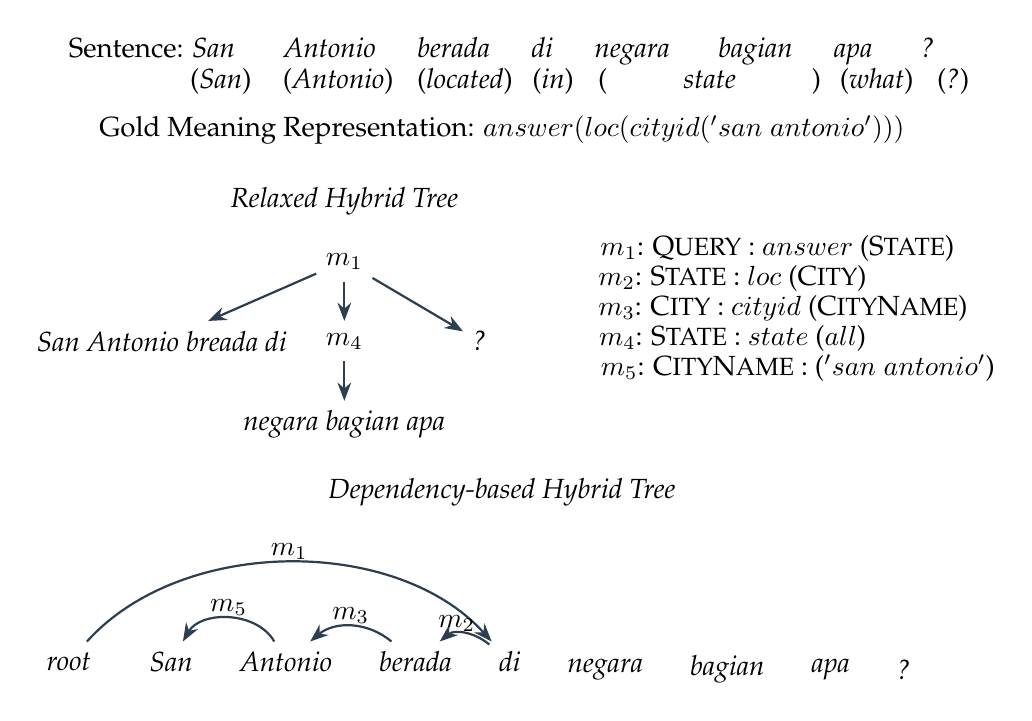
\begin{tikzpicture}[node distance=2.0mm and 2.5mm, >=Stealth, 
		semantic/.style={draw=none, minimum height=5mm, rectangle},
		word/.style={draw=none, minimum height=5mm, rectangle},
		olabel/.style={draw=none, circle, minimum height=9mm, minimum width=9mm,line width=1pt, inner sep=2pt, fill=lowblue, text=fontgray, label={center:\textsc{o}}},
		bperlabel/.style={draw=none, circle, minimum height=9mm, minimum width=9mm,line width=1pt, inner sep=2pt, fill=lowblue, text=black, label={center:\textsc{per}}},
		borglabel/.style={draw=none, circle, minimum height=9mm, minimum width=9mm,line width=1pt, inner sep=2pt, fill=lowblue, text=black, label={center:\textsc{org}}},
		bgpelabel/.style={draw=none, circle, minimum height=9mm, minimum width=9mm,line width=1pt, inner sep=2pt, fill=lowblue, text=black, label={center:\textsc{Misc}}},
		nnlabel/.style={draw=none, circle, minimum height=9mm, minimum width=9mm,line width=1pt, inner sep=2pt, fill=mypumpkin, text=black, label={center:\textsc{Gpe}}},
		invis/.style={draw=none, circle, minimum height=9mm, minimum width=9mm,line width=1pt, inner sep=2pt, fill=none, text=fontgray},
		chainLine/.style={line width=0.8pt,->, color=fontgray}	%		,background rectangle/.style={fill=olive!45}, show background rectangle
		]
		\node[semantic](sent) [] {Sentence: {\em San ~~~~~ Antonio ~~~~ berada ~~~~ di ~~~~ negara ~~~~~ bagian ~~~~ apa ~~~~~ ?}}; 
		\node[word](ew0) [below left= of sent,xshift=28.2mm,yshift=4mm] {({\em San})}; 
		\node[word](ew1) [right = of ew0, xshift=-1mm] {({\em Antonio})};
		\node[word](ew2) [right = of ew1, xshift=-2mm] {({\em located})};
		\node[word](ew3) [right = of ew2, xshift=-2.5mm] {({\em in})};
		\node[word](ew4) [right = of ew3, xshift=-1.9mm] {({\em ~~~~~~~~~~~state~~~~~~~~~~~})};
		%		\node[word](ew5) [right = of ew4, xshift=-2mm] {(})}; 
		\node[word](ew6) [right = of ew4, xshift=-2.6mm] {({\em what})}; 
		\node[word](ew7) [right = of ew6, xshift=-2mm] {({\em ?})}; 
		
		\node[word](correctsem) [below = of sent, yshift=-2mm] {Gold Meaning Representation: $answer(loc(cityid('san\;antonio')))$};
		
		\node[word](htname) [below = of correctsem, xshift=-20mm, yshift=-1mm] {{\em Relaxed Hybrid Tree}};
		
		\node[word](hm1) [below = of htname, xshift=0mm] {$m_1$};
		\node[word](hw1) [below left = of hm1, xshift=0mm, yshift=-3mm] {{\em San Antonio breada di}};
		\node[word](hw5) [below right = of hm1, xshift=9mm, yshift=-3mm] {{\em ?}};
		\node[word](hm2) [below= of hm1, xshift=0mm, yshift=-3mm] {$m_4$};
		
		%		\node[word](hm3) [below left= of hm2, xshift=-8mm, yshift=-3mm] {$m_3$};
		%		\node[word](hm4) [below = of hm2, xshift=0mm, yshift=-3mm] {$m_4$};
		\node[word](hw34) [below= of hm2, xshift=0mm, yshift=-3mm] {{\em negara bagian apa}};
		
		%		\node[word](hw2) [below= of hm3, xshift=0mm, yshift=-3mm] {{\em rivers}};
		
		%		\node[word](hm5) [below right= of hm4, xshift=5mm, yshift=-3mm] {$m_5$};
		%		\node[word](hw4) [below left= of hm5, xshift=0mm, yshift=0mm] {{\em di}};
		%		\node[word](hw56) [below left= of hm4, xshift=5mm, yshift=-3mm] {{\em titik tertinggi}};
		%		\node[word](hm6) [below= of hm5, xshift=0mm, yshift=-3mm] {$m_6$};
		%		\node[word](hm7) [below= of hm6, xshift=0mm, yshift=-3mm] {$m_7$};
		%		\node[word](hw5) [below right= of hm6, xshift=0mm, yshift=0mm] {{\em ?}};
		%		\node[word](hwiowa) [below= of hm7, xshift=0mm, yshift=-3mm] {{\em iowa}};
		
		\draw [chainLine] (hm1) to [] node[] {} (hw1);
		\draw [chainLine] (hm1) to [] node[] {} (hm2);
		\draw [chainLine] (hm1) to [] node[] {} (hw5);
		
		\draw [chainLine] (hm2) to [] node[] {} (hw34);
		%		\draw [chainLine] (hm2) to [] node[] {} (hw34);
		%		\draw [chainLine] (hm2) to [] node[] {} (hm4);
		%		
		%		\draw [chainLine] (hm5) to [] node[] {} (hw4);
		%		\draw [chainLine] (hm4) to [] node[] {} (hw56);
		%		\draw [chainLine] (hm4) to [] node[] {} (hm5);
		%		
		%		\draw [chainLine] (hm5) to [] node[] {} (hm6);
		%		\draw [chainLine] (hm6) to [] node[] {} (hm7);
		%		\draw [chainLine] (hm6) to [] node[] {} (hw5);
		%		\draw [chainLine] (hm7) to [] node[] {} (hwiowa);
		
		
		
		%		\node[word](root) [below = of dhtname, xshift=0mm] {\textit{root}};
		%		\node[word](what) [below left = of root, yshift=-3mm, xshift=-3mm] {\textit{What}};
		%		%		\node[invis](rootop) [above = of w0, yshift=8mm] {};
		%		\node[word](not) [below right = of what, xshift=15mm, yshift=3mm] {\textit{not}};
		%		\node[word](rivers) [below left = of not, yshift=-4mm] {\textit{rivers}};
		%		\node[word](through) [below right = of not, yshift=-4mm] {\textit{through}};
		%		\node[word](tennessee) [below right = of through, yshift=-4mm, xshift=-2mm] {\textit{Tennessee}};
		
		\node[word](m1)[below= of htname, xshift=55mm, yshift=2mm] {$m_1$: Q{\small{UERY}} : $answer$ (S{\small{TATE}})};
		\node[word](m2)[below= of m1, yshift=4mm, xshift=-5.7mm] {$m_2$: S{\small{TATE}} : $loc$ (C{\small{ITY}})};
		\node[word](m3)[below= of m2, yshift=4mm, xshift=6.4mm] {$m_3$: C{\small{ITY}} : $cityid$ (C{\small{ITY}}N{\small{AME}})};
		\node[word](m4)[below= of m3, yshift=4mm, xshift=-6.4mm] {$m_4$: S{\small{TATE}} : $state$ ($all$)};
		%		\node[word](m5)[below= of m4, yshift=4mm, xshift=-2.2mm] {$m_5$: P{\small{LACE}} : $loc$ (S{\small{TATE}})};
		%		\node[word](m6)[below= of m5, yshift=4mm, xshift=8.0mm] {$m_6$: S{\small{TATE}} : $stateid$ (S{\small{TATE}}N{\small{AME}})};
		\node[word](m5)[below= of m4, yshift=4mm, xshift=8.3mm] {$m_5$: C{\small{ITY}}N{\small{AME}} : ($'san\;antonio'$)};
		
		%		\Tree [.\node(root){$m_1 \equiv $ Q{\small{UERY}} : $answer$ (R{\small{IVER}})}; [.{$m_2 \equiv $ R{\small{IVER}}: $exclude$ (R{\small{IVER}}, R{\small{IVER}})} {$m_3 \equiv$ R{\small{IVER}} : $state$ (all)} [.{$m_4 \equiv$ R{\small{IVER}} : $traverse$ (S{\small{TATE}})} [.{$m_5 \equiv $S{\small{TATE}} : $stateid$ (S{\small{TATE}}N{\small{AME}})} {$m_6 \equiv$  S{\small{TATE}}N{\small{AME}} : ($'texas'$)} ]] ]]
		
		%		\draw [chainLine] (root) to [] node[above, color=black,sloped] {\small  $m_1$} (what);
		%		\draw [chainLine] (what) to [] node[above, color=black,sloped] {\small  $m_2$} (not);
		%		\draw [chainLine] (not) to [] node[above, color=black,sloped] {\small  $m_3$} (rivers);
		%		\draw [chainLine] (not) to [] node[above, color=black,sloped] {\small  $m_4$} (through);
		%		\draw [chainLine] (through) to [] node[above, color=black,sloped] {\small  $m_5$} (tennessee);
		%		\draw [line width=0.8pt,->, color=fontgray]  (tennessee) to [out=90,in=-30, looseness=5.2] node[above, yshift=-1mm, color=black, sloped]{$m_6$} (tennessee);
		
		\node[word](wroot) [below = of sent, xshift = -55mm, yshift=-70mm] {{\em root}};
		\node[word](w0) [right = of wroot, xshift=2.5mm] {{\em San}};
		%		\node[invis](rootop) [above = of w0, yshift=8mm] {};
		\node[word](w1) [right = of w0, xshift=1mm] {{\em Antonio}};
		\node[word](w2) [right = of w1, xshift=1mm] {{\em berada}};
		\node[word](w3) [right = of w2, xshift=1mm] {{\em di}};
		\node[word](w4) [right = of w3, xshift=1mm, yshift=-1mm] {{\em negara}};
		\node[word](w5) [right = of w4, xshift=1mm] {{\em bagian}};
		\node[word](w6) [right = of w5, xshift=1mm] {{\em apa}};
		\node[word](w7) [right = of w6, xshift=1mm] {{\em ?}};
		\node[word](dhtname) [below = of sent, yshift=-48mm] {{\em Dependency-based Hybrid Tree}};
		\draw [line width=0.8pt,->, color=fontgray]  (wroot) to [out=48,in=132, looseness=0.9] node[above, yshift=-1mm, color=black]{$m_1$} (w3);
		\draw [line width=0.8pt,->, color=fontgray]  (w3) to [out=140,in=40, looseness=1] node[above, yshift=-1mm, xshift=-1mm, color=black]{$m_2$} (w2);
		\draw [line width=0.8pt,->, color=fontgray]  (w2) to [out=140,in=40, looseness=1] node[above, color=black, xshift= 0mm, yshift=-1mm]{$m_3$} (w1);
		%		\draw [line width=0.8pt,->, color=fontgray]  (w2) to [out=60,in=120, looseness=1] node[above, yshift=-1mm, color=black]{$m_5$} (w3);
		%		\draw [line width=0.8pt,->, color=fontgray]  (w3) to [out=60,in=120, looseness=1] node[above, yshift=-1mm, color=black]{$m_6$} (w4);
		\draw [line width=0.8pt,->, color=fontgray]  (w1) to [out=120,in=60, looseness=1] node[above, yshift=-1mm, color=black, xshift=0mm]{$m_5$} (w0);
		\end{tikzpicture} 
	}
	%	\vspace*{-3mm}
	\caption{Example results from \textsc{DepHT} and \textsc{RHT} on Indonesian.}
	%	\vspace*{-4mm}
	\label{fig:indoerror}
\end{figure}
%caused by the incorrect alignment in relaxed hybrid tree. 
We can see the question is asking ``{\em What state is San Antonio located in?}''. 
However, the natural language word order in Indonesian is different from English, where the phrase ``{\em berada di}'' that corresponds to $m_2$ (i.e., $loc$) appears between ``{\em San Antonio}'' (which corresponds to $m_5$ -- $'san\ antonio'$) and ``{\em what}'' (which corresponds to $m_1$ -- $answer$).
Such a structural non isomorphism issue between the sentence and the semantic tree  makes the relaxed hybrid tree parser unable to produce a joint representation with valid word-semantics alignment.
This issue makes the \textsc{RHT} model unable to predict the semantic unit $m_2$ (i.e., $loc$) as \textsc{RHT} has to align the words ``{\em San Antonio}'' which should be aligned to $m_5$ before aligning ``{\em berada di}''. 
However, $m_5$ has arity 0 and cannot have $m_2$ as its child. 
Thus, it would be impossible for the RHT model to predict such a meaning representation as output.
In contrast, we can see that our dependency-based hybrid tree representation appears to be more flexible in handling such cases. 
The dependency  between the two words ``{\em di}'' ({\em in}) and ``{\em berada}'' ({\em located}) is also well captured by the arc between them that is labeled with $m_2$.
%In our  {dependency-based hybrid tree} representation below, we can {\em directly} find the words ``{\em di}'' and ``{\em berada}'' where the dependency between them is represented by $m_2$. 
% due to the ordering of words in the sentences. 
The error analysis reveals the flexibility of our joint representation in different languages in terms of the word ordering, indicating that the novel dependency-based joint representation is more robust and suffers less from language-specific characteristics associated with the data.


\paragraph{Effectiveness of dependency}
To investigate the helpfulness of the features defined over latent dependencies, we conduct  ablation tests by removing the dependency-related features. 
Table \ref{tab:ablation} shows the performance of augmenting different dependency features in our \textsc{DepHT} model with basic features. 
Specifically, we investigate the performance of head word and modifier word features (\textsc{hm}) and also the bag-of-words features (\textsc{bow}) that can be extracted based on dependencies. 
It can be observed that dependency features  associated with the words are crucial for all languages, especially the \textsc{bow} features. 
\begin{table}[t!]
	\centering
%	\setlength{\tabcolsep}{3pt} % General space between cols (6pt standard)
	\renewcommand{\arraystretch}{1} % General space between rows (1 standard)
	\scalebox{1}{
		\begin{tabular}{lcccccccc}
			\toprule
			& en & th&de&el&zh&id&sv&fa\\\midrule
			\textsc{DepHT} basic & 75.0 &82.1 & 70.4&74.6&76.1&71.9&73.9&69.3\\ 
			\textsc{basic}+\textsc{hm} feats. & 80.7 & {\bf 83.9} & {\bf 75.7} &79.2&81.1&85.0&81.1&72.5\\
			\textsc{basic}+\textsc{bow} feats. & {\bf 86.1}&83.2&73.9&{\bf 79.3}&{\bf 81.4}& {\bf 86.1} &{\bf 85.4}&{\bf 73.2} \\
			\midrule
			\textsc{DepHT} & 86.8& 81.8& 76.1 & 80.4& 81.4& 86.8& 85.4& 73.9 \\
			\bottomrule
		\end{tabular}
	}
	\vspace*{-2mm}
	\caption{$F_1$ scores of our model with different dependency features.}
	\label{tab:ablation}
	\vspace*{-3mm}
\end{table}


\paragraph{Effectiveness of neural component}
The bottom part of Table \ref{tab:nonneuralresults} shows the performance comparison among models that involve neural networks.
Our \textsc{DepHT} model with embeddings as features can outperform neural baselines across several languages (i.e., Chinese, Indonesian and Swedish). 
From the table, we can see the neural component is effective, which consistently gives better results than \textsc{DepHT} and the approach that uses word embedding features only.
\citet{susanto2017semantic} presented the \textsc{Neural HT} model with different window size $J$ for their multilayer perceptron. Their performance will differ with different window sizes, which need to be tuned for each language. 
In our neural component, we do not require such a language-specific hyperparameter, yet our neural approach consistently achieves the highest performance on 7 out of 8 languages compared with all previous approaches.
% 
%With neural component, our model 
%As both the embedding and the neural component are defined on the dependency arc, the superior results of these model variants also reveal the effectiveness of our dependency-based hybrid tree representation in semantic parsing. 
As both the embeddings and the neural component are defined on the dependency arcs, the superior results also reveal the effectiveness of our dependency-based hybrid tree representation. 

%{\color{red}
%}


\section{Conclusions}

In this work, we present a novel {\em dependency-based hybrid tree} model for semantic parsing. 
The  model captures the underlying semantic information of a sentence as latent dependencies between the natural language words. 
We develop an efficient algorithm for exact inference  based on dynamic-programming.
Extensive experiments on benchmark dataset across 8 different languages demonstrate the effectiveness of our newly proposed representation for semantic parsing.

Future work includes exploring alternative approaches such as transition-based methods
%As we regard the semantics as dependencies, we would like to explore how to employ the efficient transition-based approach
~\cite{nivre2006maltparser,chen2014fast} for semantic parsing with latent dependencies, 
applying our dependency-based hybrid trees on other types of logical representations (e.g., lambda calculus expressions and SQL~\cite{P18-1033}) as well as multilingual semantic parsing~\cite{jie2014multilingual,susanto2017neural}.

\section{Dependency-based Hybrid Tree for SQL Parsing}

As SQL is getting popular recently, one natural question to ask is that \textit{Can we solve SQL parsing with Dependency-based Hybrid Trees?} 
Because the SQL itself is actually a sequential structure but not in a tree format, it could be difficult to solve it with dependency-based hybrid trees as well as designing certain grammar structures. 
However, sequential structure is a special tree structure where each node has only one child.
It is still possible to employ the dependency-based hybrid tree models for tackling the SQL problems. 
But we need to design different grammars and hybrid pattern under such a special meaning representation. 
\chapter{Potential Research Directions} % Main chapter title

\label{Chapter7}


We propose some potential research directions by further making use of the relationship between dependencies and our downstream structured prediction tasks (i.e., NER and semantic parsing). 
Specifically, the property that ``\textit{entities often form subtrees}'' allows us to design a joint model for joint dependency parsing and named entity recognition (Section \ref{sec:jointdepner}).
On the other hand, as we show that our dependency-based hybrid trees~\cite{jie2018dependency} not only have a good performance on English but especially on other languages where word order matters~\cite{ahmad2019difficulties}. 
The natural question for NER is: \textit{Is the linear-chain structure always the best for every language?}  
By answering this question, we attempt to build the NER system exploring different graphical models besides just linear-chain structures. 
Finally, as the dependency-based hybrid trees are flexible, we could propose a universal dependency-based hybrid tree framework for different kinds of meaning representations.



\section{Joint Dependency Parsing and Named Entity Recognition}
\label{sec:jointdepner}

Dependency grammar has gained significant attention in research field thanks to its efficiency and simplicity compared to phrase-structure parsing. 
Unlike a phrase structure, there is no phrasal node in a dependency structure; each node in a dependency structure represents a word-token in a sentence except for a root node. 
Dependencies refer to both syntactic and semantic relations between nodes. Using the dependency information can enhance the performance for some tasks like named entity recognition (NER), semantic role labeling (SRL) and semantic parsing \cite{kazama2008inducing,ling2012fine,johansson2008dependency,hacioglu2004semantic,poon2009unsupervised}.  
In dependency parsing, the basic first-order model \cite{eisner1996three} is defined by a decomposition of a tree into head-modifier dependencies. 
The syntactic relationship is represented by a directed arc between a \textit{head} word and a \textit{modifier} word. The $head$ word is considered more important in this relationship and the \textit{modifier} word is supplementing the meaning of the \textit{head} word. For example, Figure \ref{fig:dependency} shows an example of a dependency structure, which contains a dependency from the head word ``$from$'' to the modifier word ``$States$'' and this dependency infers some relationship between this two words.

\begin{figure}[h]
	\centering
	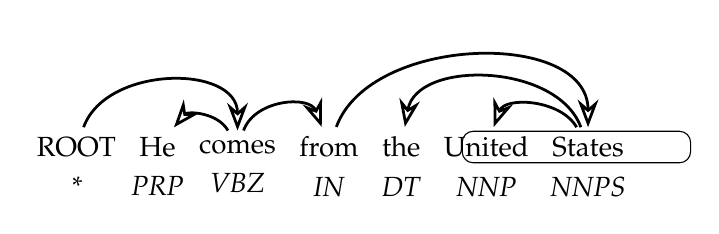
\begin{tikzpicture}[node distance=0.5mm and 0.5mm]
	\node [](root_node) at (-0.5,0) [label=below:\textit{*}]{ROOT};
	\node [](he_node) [label=below:\textit{PRP}, right=of root_node]{He};
	\node [](comes_node) [label=below:\textit{VBZ}, right=of he_node]{comes};
	\node [](from_node) [label=below:\textit{IN}, right=of comes_node]{from};
	\node [](the_node)  [label=below:\textit{DT}, right=of from_node]{the};
	\node [](united_node) [label=below:\textit{NNP}, right=of the_node]{United};
	\node [](states_node)  [label=below:\textit{NNPS}, right=of united_node]{States};
	\draw [line width=1pt, -{Stealth[length=3.5mm, open]}] (root_node) to [out=70,in=90,looseness=1.1] node [above] {} (comes_node);
	\draw [line width=1pt, -{Stealth[length=3.5mm, open]}] (comes_node) to [out=70,in=110,looseness=1.1] node [above] {} (from_node);
	\draw [line width=1pt, -{Stealth[length=3.5mm, open]}] (comes_node) to [out=120,in=50] node [above] {} (he_node);
	\draw [line width=1pt, -{Stealth[length=3.5mm, open]}] (from_node) to [out=70,in=90,looseness=1] node [above] {} (states_node);
	\draw [line width=1pt, -{Stealth[length=3.5mm, open]}] (states_node) to [out=120,in=70,looseness=1] node [above] {} (united_node);
	\draw [line width=1pt, -{Stealth[length=3.5mm, open]}] (states_node) to [out=110,in=80,looseness=1] node [above] {} (the_node);
	\draw [rounded corners] (4.4,-0.2) rectangle (7.3,0.2);
	\end{tikzpicture}
	\caption{An example dependency structure given a sentence and its POS tags. ``$United$ $States$'' is a \textit{location} entity.}
	\label{fig:dependency}
\end{figure}




However, this kind of dependency only captures the relationship between individual words while ignoring the integrity of multiple words. As in the example shown in Figure \ref{fig:dependency}, ``$United$ $States$'' is an entity with the type of \textit{location}. 
The words ``$United$ $States$'' (the rounded rectangle in Figure \ref{fig:dependency}) should be considered a group in the dependency structure. 
Thus we do not need to parse the whole entity into single words, such that we can capture the relationship between $from$ and $United$ $States$ instead of $from$ and $States$. One of the advantages of doing this is helping us to extract the predicate information like ``comes\_from(\textit{He}, /ENTITY/\textit{United States})'' in this example. 
This kind of structure with embedded entity information will further facilitate the other applications like SRL and semantic parsing. To the best of our knowledge, this is the first work focusing on the task of joint dependency parsing and named entity recognition. 
% draw a rectangle to the figure

We would like to present a new joint model for efficient dependency parsing and named entity recognition, which is a feature-based CRF model over hybrid-tree structure \cite{lu2008generative,klein2004parsing}. 
%We demonstrate our model can jointly generate consistent named entities and dependency structures. 
%We evaluate our model on the SemEval 2010 task 1 dataset which is a subset of OntoNotes 2.0 release. In general, we make the following contributions:
%\begin{itemize}
%	\item We propose a novel model that is able to jointly capture dependencies and named entity information.
%	\item We demonstrate that our model can achieve a competitive performance compared to other models doing the individual task.
%\end{itemize}
  
%\url{http://statnlp.org/research/dp/}.
\subsection{Eisner's First-order Parser}

In our joint model, we need to maintain the original dependency structure which is the first-order model introduced by \cite{eisner2000bilexical}. 
The first-order dynamic programming structure and derivation are shown in Figure \ref{fig:derivation}. 
We summarize the dynamic programming derivation here and later we can understand our joint model clearly. 
\begin{figure}[h!]
	\centering
	\begin{subfigure}{1\linewidth}
		\centering
		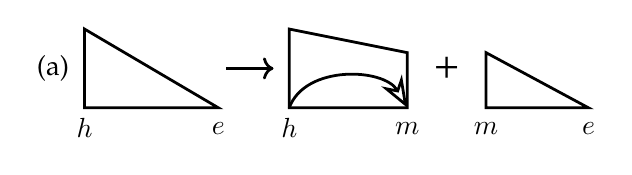
\begin{tikzpicture}
		\node [scale = 1](a) at (-0.6,0.5) {(a)};
		\draw [line width = 1pt] (1.5,0) node [below=0.05cm] {$e$} -- (-0.2,0) node [below] {$h$} -- (-0.2,1) -- cycle;
		\draw [->,line width = 1pt] (1.6,0.5) -- (2.2,0.5);
		\draw [line width = 1pt] (3.9,0) node [below=0.05cm] {$m$} -- (2.4,0) node [below] {$h$} -- (2.4,1)-- (3.9,0.7) -- cycle;
		\draw [line width=1pt, -{Stealth[length=4mm, open]}] (2.4,0) to [out=70,in=120] node [above] {} (3.9,0);
		\node [scale = 1.5](equals) at (4.4,0.5) {+};
		\draw [line width = 1pt] (6.2,0) node [below=0.05cm] {$e$} -- (4.9,0) node [below=0.05cm] {$m$} -- (4.9,0.7) -- cycle;
		\end{tikzpicture}
%		\caption{Derivation of a complete span.} 
%		\label{fig:complete}
	\end{subfigure}
	\begin{subfigure}{1\linewidth}
		\centering
		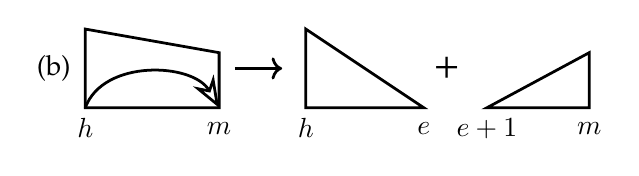
\begin{tikzpicture}
		\node [scale = 1](a) at (-0.6,0.5) {(b)};
		\draw [line width = 1pt] (1.5,0) node [below=0.05cm] {$m$} -- (-0.2,0) node [below] {$h$} -- (-0.2,1) -- (1.5,0.7) -- cycle;
		\draw [line width=1pt, -{Stealth[length=4mm, open]}] (-0.2,0) to [out=70,in=120] node [above] {} (1.5,0);
		\draw [->,line width = 1pt] (1.7,0.5) -- (2.3,0.5);
		\draw [line width = 1pt] (4.1,0) node [below=0.05cm] {$e$} -- (2.6,0) node [below] {$h$} -- (2.6,1)-- cycle;
		\node [scale = 1.5](equals) at (4.4,0.5) {+};
		\draw [line width = 1pt] (6.2,0) node [below=0.05cm] {$m$} -- (4.9,0) node [below] {$e+1$} -- (6.2,0.7) -- cycle;
		\end{tikzpicture}
%	\caption{Derivation of an incomplete span.} 
%	\label{fig:incomplete} 
\end{subfigure}
	\caption{The dynamic-programing structures and derivation of the first-order model. (a) complete span, (b) incomplete span. Only right-direction derivation is shown due to space limit. }
	\label{fig:derivation}
\end{figure}

There are two basic data structures in this dynamic-programming derivation: one is called \textit{complete} span and another one is called \textit{incomplete} span. 
A complete span, referred to Figure \ref{fig:derivation}(a), consist of a head word $h$ and a end word $e$. 
In this span, only the head word has no parent, all the other words in the span are already attached to a parent word.  
For the incomplete span, referred to Figure \ref{fig:derivation}(b), there is still a head word $h$ but the word $m$ at the other end is not complete yet. 
There is also an explicit dependency from a head word $h$ to a modifier word $m$ indicated on the span. 

Followed the notation from this work \cite{koo2010efficient}, a complete span is denoted as $C_{h,e}$ and an incomplete span is denoted as $I_{h,m}$. As shown in Figure \ref{fig:derivation}, a complete span can be decomposed to the combination of an incomplete span and a complete span. The index $m$ in Figure \ref{fig:derivation}(a) is the split point for this decomposition. An incomplete span can be decomposed to two complete spans where there is also a free index $e$ in Figure \ref{fig:derivation}(b). 
To parse a sentence into a dependency structure, we are essentially finding a construction process that can form the complete span from the first word (root) to the last word. 
The dependency structure can then be extracted from all the incomplete spans where contains an arc from the $h$ to $m$.
Using a chart-parsing algorithm like CKY can help us efficiently parse the sentence into this structure. 



\subsection{Joint Dependency and Named Entity Model}
In order to apply the dynamic programming technique in our joint model, we used similar derivation in the first-order parsing model. 
Figure \ref{fig:ourmodelderivation} shows the dynamic programming derivation of our joint model. The intuition behind is that each span in the derivation can be represented as a type, which can be \textit{person}, \textit{organization}, \textit{GPE}, \textit{MISC}. 
Besides entity type, we introduced two more types that can facilitate our model later. A type \textbf{\textit{E}} which indicates there is at least one entity inside this span and a type \textbf{\textit{N}} which indicates there is no entity inside this span. We use a label \textbf{\textit{T}} to include all this three types: \textit{E}, \textit{N} and entity types. 

In addition to complete spans and incomplete spans in the first-order model, we augmented the span type with \textit{general} spans and \textit{typed} spans. 
For a general span, there is no type information attached with it and but it has a symbol that can record its parent's type as in Figure \ref{fig:ourmodelderivation}(a) and Figure \ref{fig:ourmodelderivation}(b) the children have a symbol to store the type of their parent. 
The general spans can be decomposed to a typed span with a specific entity type as shown in Figure \ref{fig:ourmodelderivation}(a) and Figure \ref{fig:ourmodelderivation}(b). The type \textit{T}' attached with the child and the \textit{L} in the parent's symbol may not be the same since the child span might have other types that are not required to be same as the larger span. 
For example, a span (\textit{h},\textit{m}) with a type \textit{E} can have a smaller span inside that is attached with a type \textit{person}. 

Following the above example, we should define some rules that what types that smaller spans can have according to the type of their grandparents. Table \ref{tab:typerule} shows the rule that can be applied in our model. Since we can only look at the relationship between children and parent in our derivation, we are able to capture the exact relationship between a larger typed span and the two smaller typed spans which compose the larger span. 
%%%%%%%
%%%%%%%
%%%% think about how to explain this, use a figure
\begin{table}[h]
	\centering
	\begin{tabular}{cc}
		\toprule
		parent type & child type \\   \midrule
		\textit{E}' & \textit{E}, \textit{N}, \textit{person}\\ 
		\textit{N}' & \textit{N}\\
		\textit{person}' & \textit{person}\\ 
		\bottomrule
	\end{tabular}
	\caption{Derivation rule for the typed spans. Derivation for other entity types like GPE are same as \textit{person}. They are not shown in the table due to space limit.}
	\label{tab:typerule}
\end{table}
Since type \textit{E} means at least one entity inside this span, so the child type can be either \textit{E}, \textit{N} or \textit{person}. If the parent type is already \textit{N} or \textit{person}, then we define that the child type must be same as the parent type since there is also no nested entities in our dataset. 

To parse a sentence, our model tries to find an optimal construction of the sentence over all the possible hybrid-tree structure built by the derivation. 
This can be done similarly as the first-order parsing by the chart-parsing technique. 
The decomposition process (Figure \ref{fig:ourmodelderivation}(a) and \ref{fig:ourmodelderivation}(b)) of the typed span is same as first-order parsing since the entity type \textit{T} is not the free parameters like the third free index (the split point).
Since each derivation is at most defined by two fixed indices and an entity type, this parsing algorithm will need $\mathcal{O}(n^{2}|T|)$ space. The complexity of our parsing algorithm is still $\mathcal{O}(n^{3}|T|)$, where $n$ is the length of a sentence. 
\begin{figure}[h]
	\centering
	\begin{subfigure}{0.45\linewidth}
		\centering
		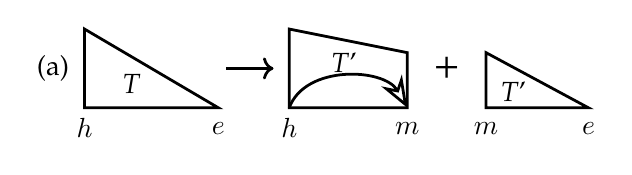
\begin{tikzpicture}
		\node [scale = 1](a) at (-0.6,0.5) {(a)};
		\draw [line width = 1pt] (1.5,0) node [below=0.05cm] {$e$} -- (-0.2,0) node [below] {$h$} -- (-0.2,1) -- cycle;
		\node [](type) at (0.4, 0.3) {\textit{T}};
		\draw [->,line width = 1pt] (1.6,0.5) -- (2.2,0.5);
		\draw [line width = 1pt] (3.9,0) node [below=0.05cm] {$m$} -- (2.4,0) node [below] {$h$} -- (2.4,1)-- (3.9,0.7) -- cycle;
		\node [](pa_type1) at (3.1, 0.57) {\textit{T}'};
		\draw [line width=1pt, -{Stealth[length=4mm, open]}] (2.4,0) to [out=70,in=120] node [above] {} (3.9,0);
		\node [scale = 1.5](equals) at (4.4,0.5) {+};
		\draw [line width = 1pt] (6.2,0) node [below=0.05cm] {$e$} -- (4.9,0) node [below=0.05cm] {$m$} -- (4.9,0.7) -- cycle;
		\node [](pa_type2) at (5.25, 0.2) {\textit{T}'};
		\end{tikzpicture}
	\label{fig:modelcomplete} 
\end{subfigure}
	\begin{subfigure}{0.45\linewidth}
		\centering
		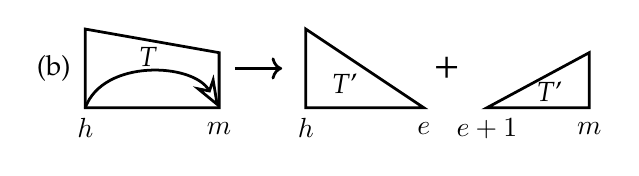
\begin{tikzpicture}
		\node [scale = 1](a) at (-0.6,0.5) {(b)};
		\draw [line width = 1pt] (1.5,0) node [below=0.05cm] {$m$} -- (-0.2,0) node [below] {$h$} -- (-0.2,1) -- (1.5,0.7) -- cycle;
		\node [](type) at (0.6, 0.65) {\textit{T}};
		\draw [line width=1pt, -{Stealth[length=4mm, open]}] (-0.2,0) to [out=70,in=120] node [above] {} (1.5,0);
		\draw [->,line width = 1pt] (1.7,0.5) -- (2.3,0.5);
		\draw [line width = 1pt] (4.1,0) node [below=0.05cm] {$e$} -- (2.6,0) node [below] {$h$} -- (2.6,1)-- cycle;
		\node [](pa_type1) at (3.1, 0.3) {\textit{T}'};
		\node [scale = 1.5](equals) at (4.4,0.5) {+};
		\draw [line width = 1pt] (6.2,0) node [below=0.05cm] {$m$} -- (4.9,0) node [below] {$e+1$} -- (6.2,0.7) -- cycle;
		\node [](pa_type2) at (5.7, 0.2) {\textit{T}'};
		\end{tikzpicture}
	\label{fig:modelincomplete} 
\end{subfigure}
	\begin{subfigure}{0.45\linewidth}
		\centering
		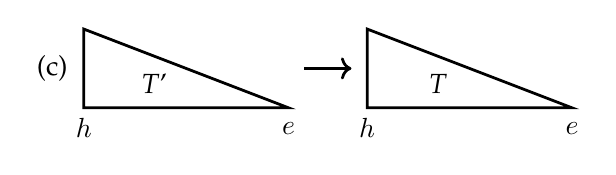
\begin{tikzpicture}
		\node [scale = 1](a) at (-0.6,0.5) {(c)};
		\draw [line width = 1pt] (2.4,0) node [below=0.05cm] {$e$} -- (-0.2,0) node [below] {$h$} -- (-0.2,1) -- cycle;
		\node [](pa_type1) at (0.7, 0.3) {\textit{T}'};
		\draw [->,line width = 1pt] (2.6,0.5) -- (3.2,0.5);
		\draw [line width = 1pt] (6.0,0) node [below=0.05cm] {$e$} -- (3.4,0) node [below] {$h$} -- (3.4,1)-- cycle;
		\node [](type) at (4.3, 0.3) {\textit{T}};
		\end{tikzpicture}
	\label{fig:generalcomplete}
\end{subfigure} 
	\begin{subfigure}{0.45\linewidth}
		\centering
		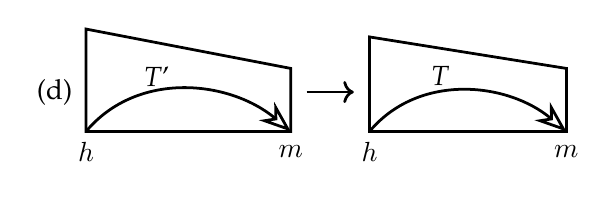
\begin{tikzpicture}
		\node [scale = 1](a) at (-0.4,0.5) {(d)};
		\draw [line width = 1pt] (2.6,0) node [below=0.05cm] {$m$} -- (0,0) node [below] {$h$} -- (0,1.3) -- (2.6,0.8) -- cycle;
		\node [](pa_type1) at (0.9, 0.7) {\textit{T}'};
		\draw [line width=1pt, -{Stealth[length=4mm, open]}] (0,0) to [out=50,in=140] node [above] {} (2.6,0);
		\draw [->,line width = 1pt] (2.8,0.5) -- (3.4,0.5);
		\draw [line width = 1pt] (6.1,0) node [below=0.05cm] {$m$} -- (3.6,0) node [below] {$h $} -- (3.6,1.2)-- (6.1,0.8) -- cycle;
		\draw [line width=1pt, -{Stealth[length=4mm, open]}] (3.6,0) to [out=50,in=140] node [above] {} (6.1,0);
		\node [](type) at (4.5, 0.7) {\textit{T}};
		\end{tikzpicture}
	\label{fig:generalincomplete} 
\end{subfigure}
	\caption{The dynamic-programming structures and derivation of our joint dependency parsing and named entity recognition model. Typed spans are decomposed to general spans and general spans are decomposed to typed spans.}.
	\label{fig:ourmodelderivation}
\end{figure}


By jointly parsing the entity and dependency together, they can interact and help each other in the joint model. 
We found that most of the named entities in our dataset have an outmost dependency that headed by either the beginning or the end of an entity. 
Inspired by this structure, we can then extract the joint features in this kind of span and as well as their entity features and dependency features. 
For example, the dependency structure of an organization entity \textit{National University of Singapore} is shown in Figure \ref{fig:jointsmallexample}.
\begin{figure}
	\centering
	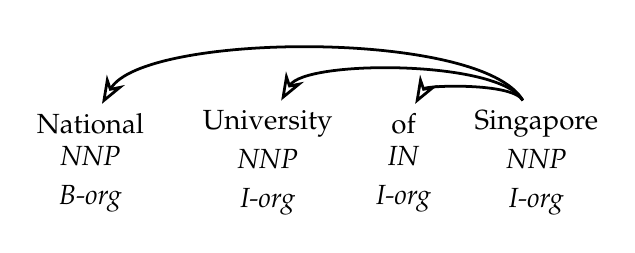
\begin{tikzpicture}[node distance=4mm and 5mm]
	\node [](a_node) []{National};
	\node [](b_node) [right=of a_node] {University};
	\node [](c_node) [right=of b_node] {of};
	\node [](d_node) [right=of c_node]{Singapore};
	\node [](at_node) [label=below:\textit{B-org},below=of a_node,yshift=5mm]{\textit{NNP}};
	\node [](bt_node) [label=below:\textit{I-org}, below=of b_node,yshift=5mm] {\textit{NNP}};
	\node [](ct_node) [label=below:\textit{I-org},below=of c_node,yshift=5mm] {\textit{IN}};
	\node [](dt_node) [label=below:\textit{I-org},below=of d_node,yshift=5mm]{\textit{NNP}};
	\draw [line width=1pt, -{Stealth[length=3.5mm, open]}] (d_node) to [out=120,in=60, looseness=0.5] node [above] {} (a_node);
	\draw [line width=1pt, -{Stealth[length=3.5mm, open]}] (d_node) to [out=120,in=60, looseness=0.5] node [above] {} (b_node);
	\draw [line width=1pt, -{Stealth[length=3.5mm, open]}] (d_node) to [out=120,in=60, looseness=0.5] node [above] {} (c_node);
	\end{tikzpicture}
	\caption{An organization entity in dependency structure.}
	\label{fig:jointsmallexample}
\end{figure}
With the derivation in Figure \ref{fig:ourmodelderivation}, the above entity forms an incomplete span from \textit{National} to \textit{Singapore}. 
This typed span is headed by \textit{Singapore} and ended at \textit{National}. 
We can then extract the whole entity features with the help of dependency information.
In a similar way, the entity information can help identify the head or modifier to find the best dependency structure. 





%\subsection{Special Case}
%\label{sec:sepcialcase}
%Following the derivation of our model, each entity with more than one word is correlated to an incomplete span in our parse tree. 
%However, not all the entities follow incomplete span structure. 
%This section will point out this case and how we try to solve them. 
%The problem is that an entity is governed by two or more spans and our model will classify each span is an unique entity, which results in one entity would be split into two span without the entity label by our model. 
%We call this case ``invalid'' span. 
%For instance, Figure \ref{fig:specialexamples} shows two example structure of this case from the training data. 
%\begin{figure*}
%	\centering
%	\begin{subfigure}{0.45\linewidth}
%		\centering
%		\begin{tikzpicture}[node distance=2.9mm and 2.9mm]
%		\node [scale = 1](a_start) [] {(a)};
%		\node [](a_node) [ right=0.5mm of a_start] {Source};
%		\node [](b_node) [right=of a_node] {$\cdots$} ;
%		\node [](c_node) [right=of b_node] {Telerate};
%		\node [](d_node) [ right=of c_node] {Systems};
%		\node [](e_node) [right=of d_node] {Inc};
%		
%		\node [](at_node) [label=below:\textit{O},below=of a_node,yshift=5mm]{\textit{NNP}};
%		\node [](bt_node) [label=below:$\cdots$ ,below=of b_node,yshift=2.5mm] {$\cdots$};
%		\node [](ct_node) [label=below:\textit{B-org},below=of c_node,yshift=5mm] {\textit{IN}};
%		\node [](dt_node) [label=below:\textit{I-org},below=of d_node,yshift=5mm]{\textit{NNP}};
%		\node [](et_node) [label=below:\textit{I-org},below=of e_node,yshift=5mm]{\textit{NNP}};
%		
%		\draw [line width=1pt, -{Stealth[length=3.5mm, open]}] (a_node) to [out=60,in=110, looseness=0.6] node [above] {} (d_node);
%		\draw [line width=1pt, -{Stealth[length=3.5mm, open]}] (d_node) to [out=120,in=60, looseness=0.6] node [above] {} (c_node);
%		\draw [line width=1pt, -{Stealth[length=3.5mm, open]}] (d_node) to [out=60,in=120, looseness=0.6] node [above] {} (e_node);
%		\end{tikzpicture}
%	\label{fig:special1} 
%\end{subfigure}
%		\begin{subfigure}{0.45\linewidth}
%			\centering
%		\begin{tikzpicture}[node distance=3mm and 3mm]
%		\node [scale = 1](b_start) [] {(b)};
%		\node [](a_node_1) [ right=of b_start] {Peoples};
%		\node [](b_node_1) [right=of a_node_1] {Drug} ;
%		\node [](c_node_1) [right=of b_node_1] {Store};
%		\node [](d_node_1) [right=of c_node_1] {Inc.};
%		\node [](e_node_1) [right=of d_node_1] {unit};
%		
%		\node [](at_node) [label=below:\textit{B-org},below=of a_node_1,yshift=5mm]{\textit{NNP}};
%		\node [](bt_node) [label=below:\textit{I-org} ,below=of b_node_1,yshift=5mm] {\textit{NNP}};
%		\node [](ct_node) [label=below:\textit{I-org},below=of c_node_1,yshift=5mm] {\textit{IN}};
%		\node [](dt_node) [label=below:\textit{I-org},below=of d_node_1,yshift=5mm]{\textit{NNP}};
%		\node [](et_node) [label=below:\textit{O},below=of e_node_1,yshift=5mm]{\textit{NNP}};
%		
%		\draw [line width=1pt, -{Stealth[length=3.5mm, open]}] (e_node_1) to [out=120,in=60, looseness=0.6] node [above] {} (a_node_1);
%		\draw [line width=1pt, -{Stealth[length=3.5mm, open]}] (e_node_1) to [out=120,in=60, looseness=0.6] node [above] {} (b_node_1);
%		\draw [line width=1pt, -{Stealth[length=3.5mm, open]}] (e_node_1) to [out=120,in=60, looseness=0.6] node [above] {} (c_node_1);
%		\draw [line width=1pt, -{Stealth[length=3.5mm, open]}] (e_node_1) to [out=120,in=60, looseness=0.6] node [above] {} (d_node_1);
%		\end{tikzpicture}
%\label{fig:special2} 
%\end{subfigure}
%	\caption{Two example of the special case from training data. The entity in (a) is split into two spans and the entity in (b) is split into four spans in our model. }
%	\label{fig:specialexamples}
%\end{figure*}
%
%As shown in Figure \ref{fig:special1}, the organization entity \textit{Telerate Systems Inc} is headed by the word inside instead of one of its boundary words. Thus this entity will be split into two spans and both of them will not be recognized as an entities when constructing the structure in our model. Similar to the second case in Figure \ref{fig:special2}, the entity in dependency structure is headed by a word \textit{unit} outside the entity. In this case, all the words of will be split into a span containing only themselves rather than form an entity span for \textit{Peoples Drug Store Inc.} 
%We do not find too many entities are forming this dependency structure in our training as shown in the experiment section. Moreover, we think a more consistent dependency structure should be headed by a boundary word as in Figure \ref{fig:jointsmallexample}. Although there are some entities are in this form which we called they are inconsistent with their dependencies. We called this kind of dependency span ``invalid'' span and found a method to solve this problem. 
%
%Since our dataset does not contain any nested named entities, we revise the model that make all the spans whose words are contained by the entity become labeled span. So that in our parsing structure of the example in Figure \ref{fig:special1}, then both of the span \textit{Telerate Systems} and \textit{Systems Inc} are labeled as organization entity. 
%We combined the entities that are near each other and have the same entity type to a single entity in a sentence. 
%Using this approach may result in another problem that not all the adjacent entities with the same type can be combined into one entity. 
%However, we found that the adjacent entities with the same entity barely appear in our data. Table \ref{tab:adjacententities} shows the number of these adjacent entities in training and testing data. This case happens only four times in training data and 2 times in testing data. Thus we ignore this kind of case and combine them into one entity in our testing result. 
%
%\begin{table}[h]
%	\centering
%	\begin{tabular}{c|cc}
%		& \multicolumn{2}{c}{\#Adjacent entities(\textit{B-E}...\textit{I-E})(\textit{B-E}} \\
%		entity & Training+Dev & Testing\\   \hline
%		\textit{person} & 0 & 0 \\
%		\textit{GPE} & 3(0.2\%) & 1(0.3\%) \\
%		\textit{organization} & 1(0.08\%) & 1(0.3\%) \\
%	\end{tabular}
%	\caption{Dataset Statistics. The number of cases that two same entities are adjacent in our dataset. }
%	\label{tab:adjacententities}
%\end{table}
%
%Our model can still handle this problem if there are nested entities in the data. If there is an entity that is split into multiple spans by the dependency structure, we split the entity into multiple entities for training. For example, the entity type for \textit{Peoples Drug Store Inc.} in Figure \ref{fig:special2} will then become \textit{B-org B-org B-org B-org} since the dependency structure will split them into four spans with only a single word.  Finally, as the statistics shown above, the adjacent entities with same type will be combined into one entity. 


\subsection{Log-Linear Modeling}
Conditional random fields (CRFs)\cite{lafferty2001conditional} have been widely used in natural language processing problems like part-of-speech tagging, named entity recognition \cite{mccallum2003early} and semantic role labeling \cite{cohn2005semantic}. 
In this work, we also defined a discriminative log-linear model over the dynamic programming derivation. 

To be more specific, the probability of predicting a possible output $\vec{y}$ (a dependency tree structure with entity information in each span) given an input sentence $\vec{x}$ is given as:
\begin{equation}
p(\vec{y}|\vec{x}) = \frac{\exp(\vec{\vec{w}^{T}\vec{f}(\vec{x},\vec{y}) })}{\sum_{\vec{y}^{'}}\exp(\vec{\vec{w}^{T}\vec{f}(\vec{x},\vec{y}^{'}) })}
\end{equation}

where $\vec{f}(\vec{x},\vec{y})$ is the feature vector defined on the sentence $\vec{x}$ and the tree structure $\vec{y}$. The best tree structure should satisfy that $\vec{y}^{*} = \argmax_{\vec{y}}p(\vec{y}|\vec{x})$. 

We aim to minimize the negative joint log-likelihood with $\textit{L}_{2}$ regularization for our dataset, which defines the objective function as:
\begin{equation}
\begin{split}
\mathcal{L}(\vec{w}) = \sum_{i}\log\sum_{\vec{y}^{'}}\exp(\vec{w}^{T}\vec{f}(\vec{x}_{i},\vec{y}^{'})) - \sum_{i}\vec{w}^{T}\vec{f}(\vec{x}_{i},\vec{y}_{i}) + \lambda \vec{w}^{T}\vec{w}
\end{split}
\end{equation} 
where $(\vec{x}_{i},\vec{y}_{i})$ is the $i$-th training instance and $\lambda$ is the $L_{2}$ regularization parameter which is set to $0.7$ in our experiments. The partial derivative of $\mathcal{L}$ with respect to each parameter $w_{k}$ is:
\begin{equation}
\begin{split}
\frac{\partial\mathcal{L}}{\partial w_{k}}  = \mathbf{E}_{p(\vec{y}^{'}|\vec{x}_{i})} \left [f_{k}(\vec{x}_{i}, \vec{y}^{'})    \right ] - \sum_{i} f_{k}(\vec{x}_{i}, \vec{y}_{i}) + 2\lambda w_{k}
\end{split}
\end{equation}
The convexity and differentiability of objective function guarantees convergence to the global optimum, and using inside-outside algorithm can efficiently compute the above gradient. There are numbers of techniques can be used for optimizing objective function. We used L-BFGS \cite{byrd1995limited} as our optimization method.

%\subsection{Features}
%For the named entity features, we applied the similar feature set from \cite{finkel2009nested}.
%The features we used are defined over the span structures as shown in our derivation of Figure \ref{fig:ourmodelderivation}. We can extract the complete entities features with the benefits of our model. The model can directly obtain the information of an entity if the span is a labeled span with entity type integrated. We applied some of the entity features from \cite{lu2015joint}. Specifically, the following features are included in our experiments: 
%\begin{itemize}
%	\item Word $n$-grams (and POS $n$-grams) that contain the current word, for $n=2,3,4$.
%	\item Boundary words (and POS tags) of the entity.
%	\item All the words (and POS tags) in the entity span.
%	\item Entity type of current span
%	\item Head or modifier word (and POS tags) with the current labeled-incomplete span
%	\item The head and modifier words (and POS tags) pair of the current labeled-incomplete span 
%\end{itemize}
%In addition to entity features, we maintained the dependency structure with the form of general span. Thus our model can extract the original dependency features which are exactly same as previous work \cite{mcdonald2005online}. Furthermore, all dependency features are conjoined with the direction of span as well as the distance between leftmost and rightmost words being attached. 
%Note that all features used in our model are the indicator functions defined on spans. But for entity features, they are also associated with their corresponding entity type.

\subsection{Preliminary Experiments}
We conduct our experiments on two datasets, one is LDC2011T01 SemEval-2010 Task 1 OntoNotes English corpus \footnote{https://catalog.ldc.upenn.edu/LDC2011T01}, which is the only one we can find has both the annotated dependency and named entity information. 
The other one is the broadcast news from LDC2013T19 OntoNotes Release 5.0 \footnote{https://catalog.ldc.upenn.edu/LDC2013T19}. Following the work on named entity recognition \cite{finkel2009joint}, we use the following 6 types of documents: ABC, CNN, MNB, NBC, PRI and VOA. 
However, there is no dependency annotation in OntoNotes 5.0 dataset. 
We applied the LTH\footnote{http://nlp.cs.lth.se/software/treebank\_converter/} converter \cite{johansson2007a} to convert the constituent parse tree to dependency structure \footnote{There are some tags (e.g. META, EDITED) from OntoNotes treebank do not appeared in the penn treebank. We removed those sentences that cannot be converted. Furthermore, we also abandon the sentences with non-projective dependency after conversion.}. 



\subsection{Dataset}
This English corpus contains both the dependency relationships and named entities information, as well as the POS tag. In general, we consider the following three entity types in the dataset: \textsc{person}, \textsc{organization}, \textsc{GPE} (geo-political entity, such as a city or a country). 
There are total 3,358 sentences for training, 684 sentences in development set and 1,058 sentences for testing. 
Since we only focus on the projective dependency parsing, the sentences with non-projective dependency are eliminated in our dataset. 

\begin{table}[h]
	\centering
	\begin{tabular}{ccccc}
		\toprule
		& \multicolumn{2}{c}{Training+Dev} & \multicolumn{2}{c}{Testing}\\ 
		& invalid & \#entity  &  invalid & \#entity  \\
		\midrule
		\textsc{per} & 18 & 1,457 & 4   & 346\\ 
		\textsc{gpe} & 41   & 1,356 & 8  & 380\\ 
		\textsc{org} & 254  & 1,199 & 69  & 382\\ 
		\#total & 313  & 4,012 & 91& 1,108\\ 
		\bottomrule
	\end{tabular}
	\caption{Dataset Statistics. The total number of entities and the number of ``invalid'' entities in training and testing data. ``Invalid`` entities are the special case describe in Section \ref{sec:sepcialcase}.}
	\label{tab:jointstatistics}
\end{table}
Table \ref{tab:jointstatistics} shows the statistics of our dataset. For ``invalid'', the entity itself cannot form a continuous subtree.
We have a total of 4,012 entities in our training and development data and 1,108 entities in testing data. 
It is obvious to see that there are few invalid entities for \textsc{person} and \textsc{gpe}. 
%Although the \textsc{organization} entity is more likely to encounter the special case in dependency structure, we can fix this problem using the trick introduced in Section \ref{sec:sepcialcase}. 

\subsection{Results}

Table \ref{tab:jointnerresult} shows the NER performance of our joint model compared to linear-chain CRF model on the SemEval 2010 dataset. 
At the moment, the results of the joint model do not surpass the performance of the linear-chain CRF model. 
Such a result gives us some guidance to further improve our model as our joint model loses some information regarding the label transition. 
\begin{table*}[h!]
	\centering
	\begin{tabular}{ccccccc}
		\toprule
		& \multicolumn{3}{c}{Just NER}  & \multicolumn{3}{c}{Our Joint Model}\\
		& Precision&Recall&F-measure & Precision&Recalll&F-measure \\ 
		\midrule
		\textsc{person}& 79.08\% & 79.77\%  & 79.42\%& 79.55\%  & 80.92\%  & 80.23\% \\
		\textsc{GPE} & 78.77\% & 87.89\% & 83.08\%  & 73.72\%  & 87.11\%  & 79.86\% \\ 
		\textsc{organization} & 67.53\%   & 54.45\% & 60.29\%  &59.01\% & 43.72\% & 50.23\% \\
		\textsc{MISC} & 80.11\%   & 63.32\% & 70.73\%   & 75.79\% & 67.69\% & 71.51\%  \\
		Overall & \textbf{76.78\%}   & \textbf{70.75\%} & \textbf{73.65\%}  & 72.87\% & 69.48\% & 71.13\% \\
		\bottomrule
	\end{tabular}
	\caption{Named Entity Recognition Results on SemEval 2010 dataset with both dependency and named entity information annotated. }
	\label{tab:jointnerresult}
\end{table*}




\section{Dependency as Graphical Models for NER}
As different languages have different word order~\cite{ahmad2019difficulties}, we believe that the classic linear-chain structures might not always be the perfect solution for NER in every language. 
To this end, we propose to use the universal dependencies as guidance for building the graphical model. 
Our goal is to build a graphical model that follows the universal dependency trees but enjoys the linear-time complexity as in the linear-chain CRF model. 




\section{Universal Hybrid Tree Framework for Semantic Parsing}

As mentioned in Chapter \ref{Chapter2}, we have many types of meaning representations such as lambda-calculus expression, FunQL, AMR, and SQL. 
However, researchers proposed different models for different types of meaning representations. 
We argue that it is not practical to have many different models in this scenario. 
In order to achieve a semantic parser that can easily adapt to different meaning representation, we propose a prototype of a dependency-based hybrid tree framework.
As the hybrid tree framework only requires hybrid tree grammar for us to build a general parser. 
We propose a series of general hybrid tree grammar that potentially apply to all types of meaning representation.

%\subsection{General Hybrid Tree Grammar}
\chapter{Conclusions} % Main chapter title

\label{Chapter8}



In this thesis, we leverage the potential of dependency trees in structured prediction tasks. 
In particular, we focus on the semantically meaningful tasks: named entity recognition and semantic parsing. 

We first present our observations from the datasets that have both named entity and dependency parse tree annotations.
Our observations suggest that most of the entities (about 99\%) in the datasets, including datasets in other languages, form contiguous subtrees in the dependency trees~\cite{jie2017efficient}. 
On the other hand, we also statistically show that certain entity types have strong correlations with some specific dependency relations~\cite{jie2019dependency}, which could be strong indicators for the existence of named entities.

Inspired by the first observation, we build an efficient dependency-guided model~\cite{jie2017efficient} based on the semi-Markov CRF~\cite{sarawagi2004semi} for named entity recognition. 
Making use of the ``\textit{subtree}'' properties, we can define certain constraints to eliminate the search space for entity candidates. 
Specifically, we can disallow some \textit{invalid} spans to become entities. 
Theoretically, we prove that our dependency-guided model achieves a linear-time complexity on average while having comparable or even better performance compared with the semi-Markov CRF model on the OntoNotes Broadcast News dataset. 


As our first approach did not fully make use of the complete dependency structures and dependency relations, we further investigate a deeper relationship between the dependency trees and named entities. 
First, the \textit{long-distance} interactions within the entity boundary are able to help us identify those long entities because such interactions \textit{shorten} the path from the entity left boundary to the right boundary. 
Secondly, the \textit{long-distance} interactions cross the entity boundary are able to help us identify the direct connection between the entity head word and the word outside entity.
Thirdly, certain entity types have strong correlations with some specific dependency relations. 
According to these properties, we propose a dependency-guided LSTM-CRF model~\cite{jie2019dependency} to capture these properties.
Empirically, the dependency-guided LSTM-CRF model achieves state-of-the-art performance on the datasets with four languages. 
Through the detailed analysis, we demonstrate that the proposed model indeed captures the properties above. 

We further present a scenario where annotations are incomplete for named entity recognition and discuss the possibility to solve the problem with a dependency-based solution.
We first argue that the current incomplete annotation scenarios are not realistic and the \textsc{o} labels should not be assumed to be available. 
This practical scenario makes the commonly used approaches such as marginal CRF~\cite{greenberg2018marginal} suffer from ``\textit{low precision and high recall}'' problem. 
We then propose an iterative training approach to address this problem and such an approach achieves much better performance compared with the strong baselines.
We also discuss the possibility of using dependency trees to help us identify those non-entity words based on the relationships mentioned above. 


Finally, we attempt to solve the semantic parsing task without explicit dependency annotations but regarding the dependency trees as a latent variable. 
Motivated by previous approaches~\cite{reddy2016transforming,wang2015building} which transform the dependency trees into meaning representations (\textit{e.g.}, lambda-calculus expression and AMR), we presented a dependency-based hybrid tree representation to jointly encode tree-structured FunQL and the natural language words. 
Such a representation is flexible in terms of word order. 
Empirically, the experimental results show the proposed hybrid tree model achieves state-of-the-art performance on 7 out of 8 languages and the improvement is significant. 
Our further analysis found that our model consistently has promising results because the proposed dependency-based representation can capture the difference of word order in different languages. 

We pose some research challenges in Chapter \ref{Chapter7} for our future research purpose. 
The challenges including a joint task for dependency parsing and NER, a task that using dependency as guidance to design a graphical model, and a universal dependency-based hybrid tree framework for different types of meaning representation in semantic parsing. 






%----------------------------------------------------------------------------------------
%	THESIS CONTENT - APPENDICES
%----------------------------------------------------------------------------------------

%\appendix % Cue to tell LaTeX that the following "chapters" are Appendices

% Include the appendices of the thesis as separate files from the Appendices folder
% Uncomment the lines as you write the Appendices

%% Appendix A

\chapter{Appendix Title Here} % Main appendix title

\label{AppendixA} % For referencing this appendix elsewhere, use \ref{AppendixA}

Write your Appendix content here.
%\include{Appendices/AppendixB}
%\include{Appendices/AppendixC}

%----------------------------------------------------------------------------------------
%	BIBLIOGRAPHY
%----------------------------------------------------------------------------------------

\printbibliography[heading=bibintoc]

%----------------------------------------------------------------------------------------

\end{document}
